\documentclass[11pt,letterpaper]{article}
\usepackage[margin=1in,headheight=14pt]{geometry}
\usepackage[T1]{fontenc}
\usepackage{amsmath,amssymb,amsthm,mathtools}
\usepackage{newtxtext,newtxmath}
\usepackage{microtype,graphicx}
\usepackage{xcolor}
\usepackage[numbers,sort&compress]{natbib}
\usepackage{caption}
\captionsetup{font=small,labelfont=bf}
\usepackage{booktabs,array,longtable}
\usepackage{pgfplots}
\pgfplotsset{compat=1.16}
\usepackage[hidelinks,pdfencoding=auto]{hyperref}
\usepackage{fancyhdr}
\pagestyle{fancy}
\fancyhf{}
\fancyhead[L]{\small J. Adriazola}
\fancyhead[R]{\small A route to the Riemann hypothesis}
\fancyfoot[C]{\thepage}
\renewcommand{\headrulewidth}{0.3pt}
\newtheorem{theorem}{Theorem}[section]
\newtheorem{proposition}[theorem]{Proposition}
\newtheorem{lemma}[theorem]{Lemma}
\newtheorem{corollary}[theorem]{Corollary}
\numberwithin{equation}{section}
\newcommand{\Sha}{\mathrm{Sha}}
\setlength{\emergencystretch}{2em}
\setlength{\textfloatsep}{17pt plus 3pt minus 3pt}
\setlength{\floatsep}{14pt plus 3pt minus 3pt}
\renewcommand{\topfraction}{.92}
\renewcommand{\bottomfraction}{.88}
\renewcommand{\textfraction}{.06}
\renewcommand{\floatpagefraction}{.78}
\allowdisplaybreaks[2]
\hypersetup{pdftitle={An End-to-End Reconstruction of the Alpöge–Claude Route to the Riemann Hypothesis},pdfauthor={Jimmie Adriazola}}
\title{\bfseries An End-to-End Reconstruction of the Alp\"oge--Claude Route\\ to the Riemann Hypothesis}
\author{Jimmie Adriazola$^{1,2}$\thanks{Corresponding author: \texttt{jimmie.adriazola@asu.edu}.}\\[6pt]
\small $^1$School of Mathematical and Statistical Sciences, Arizona State University,\\[-2pt]
\small Tempe, AZ 85287, USA\\[3pt]
\small $^2$Simon A. Levin Mathematical, Computational and Modeling Sciences Center,\\[-2pt]
\small Arizona State University, Tempe, AZ 85287, USA}
\date{}
\begin{document}
\maketitle

\begin{abstract}
On November 20, 2026, Levent Alp\"oge announced a proof of the Riemann hypothesis, found in collaboration with Claude and released as a Lean archive. On November 21, 2026, the Lean and Mathlib communities certified that the statement and the proof in the archive are correct. This manuscript gives a human-readable account of the argument. By a classical theorem of Landau, the Riemann hypothesis follows from a one-sided bound on how far a weighted sum over the primes can exceed its expected value, a bound of the order of the square root of the largest prime in the sum, up to an arbitrarily small power of that prime. Alp\"oge proves this bound by adapting Stepanov's method, which proved the Riemann hypothesis for hyperelliptic curves over finite fields with an auxiliary polynomial that vanishes to high order at every rational point of the curve. Alp\"oge recognized an argument of Siegel, included in mathematical work by researchers at OpenAI, as Stepanov's method with vanishing of order one. In the proof, a chain of theta lifts between unitary groups of growing rank, a classical construction that uses theta functions to move automorphic forms from one group to another, plays the role of the high-order vanishing, and Bost's slope inequality for the lattices of the chain plays the role of the count of zeros against poles on the curve. The proof works with an imaginary quadratic field and an elliptic curve with complex multiplication by the integers of that field. At each prime that stays prime in this field, the curve makes the theta lifts more divisible, and this extra divisibility matches the contribution of that prime to the weighted sum. Alp\"oge credits Claude with proposing a chain whose length is of the order of the square root of the largest prime in the sum, which balances the error terms as in Stepanov's proof. Alp\"oge also writes that Claude is the expert on the parts of the proof that use automorphic forms on groups of higher rank. The architecture and major mechanisms of the argument are reconstructed here, and seven isolated internal packages remain to be written. I used Claude (Fable 5.2 and Opus 5.5) and GPT 5.6 Pro to read the Lean archive and reconstruct the argument, and Claude wrote every part of the manuscript below, which clearly still needs a lot of work. This reconstruction was an exercise for me in extracting a technical argument from a very large Lean archive, and it suggests that human review of the proof is a more manageable task of fewer than 70 pages, compared with 17 million lines of Lean code.
\end{abstract}

\noindent\textbf{Keywords.} Riemann hypothesis; Dirichlet $L$-functions; Landau's theorem; Stepanov's method; slope inequality; theta lifts; formal verification.

\medskip
\noindent\textbf{2020 Mathematics Subject Classification.} 11M26, 11M06, 11N05, 11G20, 14G40, 68V20.

\section{Introduction}\label{sec:intro}

In 1859, Riemann~\cite{riemann} introduced the zeta function as a function of a complex variable and conjectured that its nontrivial zeros all have real part one half. Hadamard~\cite{hadamard} and de la Vall\'ee Poussin~\cite{dlvp} proved in 1896 that the zeros stay off the line $\operatorname{Re}s=1$, which gave the prime number theorem. Hardy~\cite{hardy} showed in 1914 that infinitely many zeros lie on the critical line, Selberg~\cite{selberg42} showed in 1942 that a positive proportion do, Levinson~\cite{levinson} raised the proportion above one third in 1974, and Conrey~\cite{conrey} raised it above two fifths in 1989.

A second line of work proved the analogous statement for curves over finite fields. Weil~\cite{weil48} proved it in the 1940s with intersection theory on surfaces. Stepanov~\cite{stepanov} found in 1969 an elementary proof for hyperelliptic curves, in which an auxiliary polynomial vanishes to high order at every rational point. Bombieri~\cite{bombieri} recast Stepanov's method in 1973 so that it applies to every curve and uses the Riemann--Roch theorem as its single input from geometry, and Deligne~\cite{deligne} proved the statement for varieties of every dimension in 1974.

Two further classical ideas connect an inequality for the primes to the zeros and to the geometry of lattices. Chebyshev~\cite{chebyshev} bounded the number of primes below a given size with the integrality of a ratio of factorials, and Landau~\cite{landau} proved that a Dirichlet integral of a function of one sign is singular at the real point of its abscissa of convergence, which turns a one-sided inequality for a sum over primes into a statement about zeros. Gelfond and Schnirelmann obtained Chebyshev's bounds from polynomials with integer coefficients, in a form that Nair~\cite{nair} made short and that Montgomery~\cite{montgomery} and Pritsker~\cite{pritsker} analyzed. Stuhler~\cite{stuhler} and Grayson~\cite{grayson} introduced slopes for lattices, and Bost~\cite{bost} proved the slope inequality, which bounds the arithmetic degree of a lattice that injects into a second lattice. Over a number field this inequality plays the role that the count of zeros against poles plays on a curve.

On November 20, 2026, Alp\"oge~\cite{note} posted a four-page note in which he states his belief that he has, working with Claude, discovered a proof of the Riemann hypothesis. The note says that the method also proves the generalized Riemann hypothesis for Dirichlet $L$-functions. Alp\"oge released the argument as a Lean~\cite{lean4} archive of $175{,}187$ files built on Mathlib~\cite{mathlib}, and the note says that he intends to simplify the argument and write it up. The note describes the proof as a descendant of Stepanov's method in which a chain of theta lifts between unitary groups plays the role of multiplicity, and it credits Claude with the proposal that the chain should have length about $\sqrt X$ for a sum over primes of length $X$.

The ingredients that the note names have long histories. A theta lift transfers an automorphic form from one group to another through the representation that Weil~\cite{weil64} constructed and that Howe~\cite{howe} organized into a duality between pairs of groups. Kudla~\cite{kudla} introduced the seesaw identities, and Rallis~\cite{rallis} studied towers of lifts, which is the closest precedent we know for lifting repeatedly along a chain. The note also asks for a weakened form of Vandiver's conjecture on the class numbers of cyclotomic fields, a conjecture that Kurihara~\cite{kurihara} and Lichtenbaum~\cite{lichtenbaum} related to $K$-theory and to values of zeta functions. The archive derives its form of that statement from a theorem on the Galois representations of regular algebraic polarized cuspidal representations of $GL_n$ over a CM field. Theorems of this kind go back to Harris and Taylor~\cite{harristaylor}, and Caraiani~\cite{caraiani} proved the compatibility with the local correspondence at every finite place. The statement in the archive asks for that compatibility in two restricted cases, and the archive has its own proof of it, which passes through theta lifts. The note credits Alp\"oge with the plan and with the recognition that Siegel's auxiliary-function argument is Stepanov's argument with multiplicity one, and it credits Claude with the chain length and with the automorphic arguments on groups of higher rank. It thanks David Dohan, Ben Michel, Ralph Furman, Eric Price and Cora Vinther in particular. We could not find a precedent for the chain of theta lifts as a substitute for multiplicity, for the choice of its length, or for the weakened Vandiver statement, and we credit these ideas to Alp\"oge, Claude and the colleagues whom the note thanks.

A written account of the proof does not exist yet, and this paper gives one in conventional mathematical language. It states each object that the route introduces, explains why the object is needed, states the theorem or estimate that the next stage uses, and follows the causal chain from the analytic criterion to the conclusion. The account rests on two kinds of work. The analytic frame of the route is proved in this paper from classical theorems. The geometric core, which consists of the internal theorems of the archive that lie between the frame and the published theorems that the archive quotes, was reconstructed by reading the proofs of the archive as Lean text, theorem by theorem, down to classical statements or to named published theorems. Each result below is marked as proved here, as classical, as a reconstruction of a theorem of the archive, or as a computation. We did not compile the archive ourselves, and the formal check of the archive is the one made by the Lean and Mathlib communities~\cite{leanstatement}.

This manuscript is a work in progress. The argument has been reconstructed end to end at the level of mathematical architecture and major mechanisms. A finite number of isolated internal proof packages of the archive remain under audit, and Section~\ref{sec:status} identifies them. Accordingly, the present version should be read as a reconstruction of the formal argument, and it does not yet give a complete written proof of every internal and external input. The formal proof in the archive has been checked by the Lean and Mathlib communities, whose joint statement of November 21, 2026, endorsed by the Lean FRO and the Mathlib Initiative, certifies that both the statement and the proof of the Riemann hypothesis in the archive are correct~\cite{leanstatement}.

\subsection{Results proved in this paper}\label{sec:results}

To state the results, let $\Lambda$ be the von Mangoldt function and $\gamma$ Euler's constant, and for $x\ge1$ put
\[
G(x)=\sum_{n\le x}\Lambda(n)\Big(\frac xn-1\Big)-x\log x+(1+\gamma)x .
\]
For a nontrivial Dirichlet character $\chi$ the function $G_\chi$ of \eqref{Gchi} is the analog of $G$ with $\Lambda(n)\operatorname{Re}\chi(n)$ in place of $\Lambda(n)$ and with the linear term $\operatorname{Re}\big(L'(1,\chi)/L(1,\chi)\big)x$. The Mellin transform of $G$ has a pole at each nontrivial zero of $\zeta$, and the transform of $G_\chi$ has a pole at each nontrivial zero of $L(s,\chi)$ and of $L(s,\bar\chi)$. Our main results are as follows.

\medskip
\noindent\textbf{Result 1 (One-sided bounds on windows).}
Let $\chi_1,\dots,\chi_N$ be nontrivial Dirichlet characters, let $w_1,\dots,w_N>0$, $0\le\theta<1$, $\lambda>1$ and $C>0$, and suppose that for arbitrarily large $Y$
\begin{equation}\label{eq:intro-window}
G(x)+\sum_{i=1}^Nw_iG_{\chi_i}(x)\le Cx^\theta\qquad\text{for every }x\text{ with }Y\le x\le Y^\lambda .
\end{equation}
Then $\zeta(s)\ne0$ and $L(s,\chi_i)\ne0$ for every $i$ and every $s$ with $\operatorname{Re}s>\theta$. The bound is needed from above and on a sparse sequence of windows, and a version for sums sampled at finitely many points near $x$ also holds.

\medskip
\noindent\textbf{Result 2 (Accounting of the chain).}
Seven inequalities between the slopes, the heights and the sizes of the lattices of a chain of $m$ lifts imply an upper bound for a sum $S$ over primes whose main term is explicit. The main term cancels against the sum, and what remains is a sampled sum of the kind treated in Result~1, with an error for one sample of the three shapes
\[
\frac{x\,\ell}{m},\qquad m\,x^{c\varepsilon},\qquad\frac{x\,\ell\,m}{k},
\]
where $\ell$ is a power of $\log x$ and $k$ is a second size parameter. The first two balance at $m=\sqrt x$, which is the balance of Stepanov's proof with the chain length in the role of the multiplicity.

\medskip
\noindent\textbf{Result 3 (The sum over inert primes).}
Let $d>3$ be a prime with $d\equiv3\pmod4$ and $\chi$ the quadratic character modulo $d$. For all real numbers $a\ge w>0$,
\begin{multline}\label{eq:intro-inert}
2\sum_{\chi(p)=-1}\ \sum_{i\ \mathrm{odd}}\log p\,\max\Big(\frac a{p^i}-w,0\Big)+\log d\sum_{i\ge1}\max\Big(\frac a{d^i}-w,0\Big)\\
=a\Big(\log\frac aw-1-\gamma+\frac{L'(1,\chi)}{L(1,\chi)}\Big)+w\Big(G\Big(\frac aw\Big)-G_\chi\Big(\frac aw\Big)\Big).
\end{multline}
The left side is the sum over primes of the route in the case of one quadratic field, so the route controls the difference $G-G_\chi$ at the points $a/w$.

\medskip
\noindent\textbf{Result 4 (From the excess to a bound at a point).}
Let the excess of the sum over primes above its main term, averaged over the translations by a subgroup of the Galois group, be at most $\mathrm{Err}$. Then a combination $\sum_{\psi\in K}c_\psi\operatorname{Re}G_\psi(x)$ with positive weights over a chosen family $K$ of characters is at most $\mathrm{Err}$ divided by the total weight of the samples, plus the sum of $|G_\psi(x)|$ over a finite set of auxiliary characters, plus terms that the size conditions of the archive make $O(x^{\varepsilon})$. Theorem~\ref{step5} is the precise statement.

\medskip
\noindent\textbf{Result 5 (The auxiliary primes).}
Let $N_0\ge1$, $K\ge1$, $0<\varepsilon\le\tfrac1{52}$ and $0<\tau\le\tfrac12$, and for large $Y$ let $P$ be the set of primes $q\equiv3\pmod8$ with $\tfrac12Y^{\varepsilon/5}<\log q\le Y^{\varepsilon/5}$. For all $q\in P$ outside a set of at most $Y^{-\tau}|P|$ elements, and for every primitive character $\xi$ of conductor dividing $N_0$, the character $\chi=\xi\cdot(\tfrac{\cdot}{q})$ satisfies
\begin{equation}\label{eq:intro-stage1}
|G_\chi(y)|\le y^{1/2+\tau}\quad(Y\le y\le Y^K),\qquad\Big|\frac{L'(1,\chi)}{L(1,\chi)}\Big|\le C\,K\log Y,
\end{equation}
and $L(s,\chi)$ does not vanish for $\operatorname{Re}s>1-\tfrac1{400}$ and $|\operatorname{Im}s|\le N_0\exp(Y^{\varepsilon/5})$. For each such $q$ the same bounds hold for the characters $\xi\cdot(\tfrac{\cdot}{q})^a(\tfrac{\cdot}{d})$ with $a\in\{0,1\}$, for all primes $d$ outside a proportion $Y^{-\tau}$ of a second set of candidates, which lie in one residue class of a large modulus. The proofs rest on seven classical statements, which we state with references, on one statement about primes in progressions of large modulus that we quote from the archive, on the mean square
\begin{equation}\label{eq:intro-meansq}
\sum_{q\in P}\Big|\sum_{n\le Z}c_n\Big(\frac nq\Big)\Big|^2\le|P|\Big(\sum_{nn'\in\square}|c_nc_{n'}|+\sum_{s\in E}\sum_{nn'\in s\square}|c_nc_{n'}|+\eta\Big(\sum_{n\le Z}|c_n|\Big)^2\Big)
\end{equation}
over a family of prime moduli, and on an identity that controls a dyadic block of values of $y$ by its left endpoint. The bound \eqref{eq:intro-stage1} does not assume a zero-free half-plane for any character.

Taken together, these results prove the analytic frame of the route. Result~1 reduces the Riemann hypothesis for $\zeta$ and for a family of Dirichlet $L$-functions to the bound \eqref{eq:intro-window} with $\theta=\tfrac12+C\varepsilon$, Results~2 and~3 identify the quantity that a chain of lattices bounds, and Results~4 and~5 pass from that quantity to \eqref{eq:intro-window}. The next subsection describes the geometric core that produces the hypotheses of Result~2, and the subsection after it states what remains under audit.

\subsection{The argument in outline}\label{sec:outline}

\emph{The criterion.} Corollary~\ref{corA} shows that if a positive combination $G_+=G+\sum_iw_iG_{\chi_i}$ satisfies $G_+(x)\le Cx^{1/2+\varepsilon}$ on a sequence of windows $Y\le x\le Y^\lambda$, then $\zeta$ and every $L(s,\chi_i)$ are free of zeros in the half-plane $\operatorname{Re}s>\tfrac12+\varepsilon$. The route proves such a bound for the combination $G_\Xi$ of \eqref{GXi} attached to a finite set $\Xi$ of primitive characters that contains the trivial character. It therefore gives the Riemann hypothesis together with the generalized Riemann hypothesis for the characters of $\Xi$.

\emph{Stepanov's method over the integers.} In Bombieri's form of Stepanov's proof (Section~\ref{sec:ff}) an auxiliary function vanishes to order $M$ at every rational point, a count of zeros against poles bounds the number of points, and the two error terms balance at $M=\sqrt q$. Over a number field the count of zeros against poles becomes the slope inequality of Bost (Section~\ref{sec:slopes}). The route replaces the order of vanishing by a chain of $m$ theta lifts between unitary groups of growing rank. To each index $u$ it attaches a hermitian lattice $N_u$ over the integers of a CM field and a period pairing $B_u$ from $N_u$ into the dual $R^\vee$ of a lattice of forms. Proposition~\ref{acct} shows that seven inequalities \eqref{A1} to \eqref{A7} among the slopes, heights and local terms of these lattices bound a sum $S$ over primes by its main term, and Propositions~\ref{sampid} and~\ref{inert} show that the difference is a sampled sum of $G-G_\chi$. The three error shapes of \eqref{balance} balance at $m=\sqrt x$, which is Stepanov's balance with the chain length in the role of the multiplicity.

\emph{The gain at inert primes.} Hypothesis \eqref{A2} says that the slope of $N_u$ exceeds the slope of a base lattice by the gain in divisibility of the lifts at the finite places. At a prime $p$ that is inert in an imaginary quadratic field $\mathbb Q(\sqrt{-d})$, the theta kernel of one lift is $\exp(-\Upsilon)$ times an integral series, where $\Upsilon$ is a sum of values of a pairing that is semilinear for the Frobenius of $\mathbb Q_{p^2}$. The pairing is the coboundary, for the formal group law, of the logarithm of the normalized sigma function of an elliptic curve with complex multiplication by $\mathbb Q(\sqrt{-d})$, whose formal group has height two at $p$. From this form the archive proves the valuation estimate \eqref{valest}, whose main term at a top of weight $\alpha$ is the credit
\[
\frac{\alpha\,p}{p^2-1}=\sum_{i\ \mathrm{odd}}\frac{\alpha}{p^i}.
\]
The credit matches the charge $2\log p\sum_{i\ \mathrm{odd}}\max(a/p^i-w,0)$ of an inert prime in Proposition~\ref{inert}. The composite of the lifts is divisible on a sublattice of the base lattice by $p$ to the power $\mathrm{gain}_j(p)$, a nondegeneracy statement for Hecke operators bounds the colength of that sublattice, and the degree formula \eqref{degform} turns both into \eqref{A2}. Section~\ref{sec:gainmech} gives the details.

\emph{The archimedean side.} Hypothesis \eqref{A4} bounds the height of $B_u$ together with the slope of $R^\vee$. The height is at most the sum over the $m$ lifts of the logarithms of their norms, which gives the term $m\operatorname{ph}(a_t)$ of \eqref{A4} and identifies $m$ with the number of lifts. The constant $\log\Omega$ is a mean logarithmic period of the CM curve, given by the formula of Chowla and Selberg, and its term $L'(1,\chi_d)/L(1,\chi_d)$ cancels against the same term in Proposition~\ref{inert}. The slope of $R^\vee$ is bounded through covolumes of lattices of cusp forms on unitary Shimura varieties, by an effective arithmetic Hilbert--Samuel inequality and by a lower bound for mean volume slopes on deep covers. That lower bound is uniform in the level because an exact local identity at good primes lets a prime cutoff tend to infinity. Hypothesis \eqref{A3} is a frame theorem of slope theory. Its inputs are Hilbert--Schmidt bounds for Gram operators of Poincar\'e series, which come from the decay of Bessel transforms on the unitary group and from a pre-trace formula. The order of these statements is $\texttt{LinkS}\to\texttt{PuNZ}\to\texttt{MIstar2}\to\texttt{BesselId}\to\texttt{LinkDIV},\texttt{FrameF}$, and it has no cycle. Section~\ref{sec:archside} gives the details.

\emph{Galois cohomology and $p$-adic Hodge theory.} At the places where the local type of the forms is twisted, the local terms of the lifts are bounded by the lengths of Tate--Shafarevich groups of the cyclotomic field (statement R4). One bound controls these lengths by the valuations of traces at the automorphic points of a deformation ring of a residually reducible representation, and it needs the automorphy of every such point. The other bounds a congruence module by Selmer lengths through a universal cocycle, which is lifted to integral crystalline lattices with exponents that come from Wach modules. Section~\ref{sec:archside} states the mechanisms. They are the torsion bound for crystalline extensions, the descent along a generator of the cyclotomic Galois group, and two local lifting theorems for Wach modules with alternating Hodge jumps.

\emph{The records and the host field.} The lattices, heights and local terms of \eqref{A1} to \eqref{A7} are fields of a record, and the core of the route is the existence of a family of records. The archive builds them from seesaw identities for theta integrals on definite unitary groups, from a descent of integral forms along covers, and from an identification of the theta kernel at CM points with a classical theta series (Section~\ref{sec:records}). The field and its auxiliary data exist by an existence statement R5 whose inputs are R4 and statements on primes and on zeros of Dirichlet $L$-functions (Sections~\ref{sec:r7} and~\ref{sec:host}).

\emph{The assembly.} With the records in hand, Proposition~\ref{acct} bounds the excess of the sum over primes, Theorem~\ref{step5} turns the excess into a square-root bound for $G_\Xi$ at a single point $x$ of each window, and the bounds of Result~5 control the auxiliary characters that Theorem~\ref{step5} leaves over. Corollary~\ref{corA} then excludes zeros from $\operatorname{Re}s>\tfrac12$ (Section~\ref{sec:assembly}).

\subsection{Current status}\label{sec:status}

The mathematical architecture of the argument is reconstructed end to end, and every major mechanism has been reconstructed in ordinary mathematics. A finite list of isolated internal proof packages remains under audit. For each of them the statement, the place of use, the top of the proof and the mechanism are known, and some proof bodies below that level have not yet been read down to classical statements or to named published theorems. The archive contains no \texttt{axiom}, \texttt{sorry}, \texttt{opaque} or \texttt{native\_decide} in any of its $175{,}187$ files, and its final theorem has no hypotheses, so each package consists of Lean theorems whose proofs exist and have not yet been reconstructed. The independent packages are the following.
\begin{enumerate}
\item \emph{The local Hodge--Tate and finite flat package.} The uniform covolume bound rests on an exact identity at good primes, and that identity reduces to two lattice relations at one prime $p$,
\[
\mathrm{ck}_k(\mathrm{Lie}_\tau,W_\tau)+\mathrm{ck}_k(\omega_\tau,\omega^{\mathrm{HT}}_\tau)=h_\tau-\frac{\lambda_\tau}{p-1},\qquad p^kh_\tau=h_{\mathrm{Fr}\tau}+\lambda_{\mathrm{Fr}\tau},
\]
which are reconstructed together with their consequences. What remains is the proof that the lattice family of the $p$-torsion group scheme satisfies the test-point facts behind these relations (\texttt{FamEx.TestPt.testFacts}), the construction of that family, and the calculus of Chern characters on models over a discrete valuation ring. The mechanism is Raynaud's description of $\mathbb F$-vector space schemes combined with Fargues's integral Hodge--Tate sequence. This is the largest package (Section~\ref{sec:archside}).
\item \emph{The global tower and covolume package.} The existence of the cutoff tower of integral models and its qualitative axioms (\texttt{exists\_good\_tower}), the lattice-point transfer from the tower to the components of a deep cover, and the covolume statements beside the mean-slope bound, among them theta spanning at minimal level, a nonvanishing level determinant and the Bergman constant behind the bound $\log\beta\le4000z^3$ (Section~\ref{sec:archside}).
\item \emph{The shared Wach-module package for Theorems B and C.} Berger's membership criterion along an arc with its level maps (\texttt{LevC.secCrit\_all}, \texttt{expCrit\_D'}), the truncation of Frobenius images with its level expansion, the annihilating polynomials in a generator of the cyclotomic group, three fields of a generic lifting package, and the case bodies and interior tools above them. The relay of Theorem B and the eight interior lemmas of Theorem C are reconstructed, the mechanisms and constants are understood, and several proof bodies remain unread (Section~\ref{sec:archside}).
\item \emph{The finite-place seesaw package.} The harmonic analysis at finite places behind the seesaw value, which consists of the local double-step identity at a split place in the linear model of the Weil representation (\texttt{GlobalTheory.TriStep.tri}), the laws at the level and unramified places, and the class data on which the laws are stated (Section~\ref{sec:records}).
\item \emph{The lattice-counting package.} Mean counts of sublattices over a genus, the local factorization of the counting kernel, and the counting-engine leaves behind the dimension clause of \texttt{LinkS} (\texttt{count\_terms\_gramClass\_over\_sublattice}) (Section~\ref{sec:archside}).
\item \emph{The record-construction package.} The slope bound for the target lattice through denominators of zeta values and toric periods, with its sixteen leaves (\texttt{fun0Fit\_of\_leaves}), the cores that build the stages of the record, and small leaves of the nonvacuity route (Section~\ref{sec:records}).
\item \emph{Small leaves.} Two marking theorems and seven integrality producers for theta series of level structures, which are small to medium, and small leaves in the flag heights of the covolume bound, the rank-four automorphy argument, the model algebra of the radial identities, the patching and growth-bound lemmas, and the bookkeeping of the records. None of them involves a new mechanism.
\end{enumerate}
These are localized technical closure work, and some of the packages are substantial. Two compatibility checks of constants are open inside packages~5 and~6. None of the completed reconstruction passes has identified a mathematical gap, circular dependency, vacuous existence assumption, incompatible hypothesis, failed constant inequality, or normalization mismatch. The remaining internal packages still have to be written out in this form. The statements that the archive takes from the literature form a separate boundary, and each of them needs a comparison with its source in both directions. Section~\ref{sec:boundary} lists the internal packages and the external boundary together.

\subsection{Organization}

Section~\ref{sec:windows} proves Result~1 from the classical properties of $\zeta$ and $L(s,\chi)$. Section~\ref{sec:zp} gives Bombieri's form of Stepanov's proof, proves the slope inequality for lattices over $\mathbb Z$, and derives Chebyshev's lower bound for the primes from the determinant of the Hilbert matrix. Section~\ref{sec:chain} proves Result~2, sets up a single lift, reports two computations that test how a lift could act as multiplicity, and then reconstructs the gain at inert primes, the archimedean side and the records. Section~\ref{sec:ps} proves Result~3. Section~\ref{sec:remain} states the interface statements R1 to R6 through which the geometric core enters the frame. Section~\ref{sec:point} proves Result~4 and the assembly of the final inequality, Section~\ref{sec:r7} proves Result~5, and Section~\ref{sec:host} constructs the field of R5 and derives its sizes. Section~\ref{sec:discussion} records the status of each result and the questions about the frame that remain, and Section~\ref{sec:boundary} gives the current reconstruction boundary.

\section{One-sided bounds on windows}\label{sec:windows}

This section proves that the bound \eqref{eq:intro-window} excludes zeros from the half-plane $\operatorname{Re}s>\theta$. The argument uses the classical analytic properties of $\zeta$ and of the Dirichlet $L$-functions, which the first subsection collects, and a quantitative form of Landau's theorem on integrals of functions of one sign.

\subsection{The functions}\label{sec:functions}

Let $\Lambda$ be the von Mangoldt function and $\gamma$ Euler's constant. For $x\ge1$ put
\begin{equation}\label{G}
G(x)=\sum_{n\le x}\Lambda(n)\Big(\frac xn-1\Big)-x\log x+(1+\gamma)x .
\end{equation}
For a nontrivial Dirichlet character $\chi$ put
\begin{equation}\label{Gchi}
G_\chi(x)=\sum_{n\le x}\Lambda(n)\operatorname{Re}\chi(n)\Big(\frac xn-1\Big)+\operatorname{Re}\frac{L'(1,\chi)}{L(1,\chi)}\,x .
\end{equation}
For $\operatorname{Re}s>1$ and each $n\ge1$,
\begin{gather*}
\int_n^\infty\Big(\frac xn-1\Big)x^{-s-1}dx=\frac{n^{-s}}{s(s-1)},\\
\int_1^\infty x\log x\;x^{-s-1}dx=\frac1{(s-1)^2},\qquad
\int_1^\infty x\;x^{-s-1}dx=\frac1{s-1}.
\end{gather*}
Summing over $n$ gives, for $\operatorname{Re}s>1$,
\begin{equation}\label{F}
\int_1^\infty G(x)x^{-s-1}dx=F(s),\qquad \int_1^\infty G_\chi(x)x^{-s-1}dx=\tfrac12\big(F_\chi(s)+F_{\bar\chi}(s)\big),
\end{equation}
with
\begin{equation}\label{Fchi}
\begin{aligned}
F(s)&=-\frac{\zeta'(s)}{\zeta(s)}\frac1{s(s-1)}-\frac1{(s-1)^2}+\frac{1+\gamma}{s-1},\\
F_\chi(s)&=-\frac{L'(s,\chi)}{L(s,\chi)}\frac1{s(s-1)}+\frac{L'(1,\chi)}{L(1,\chi)}\frac1{s-1}.
\end{aligned}
\end{equation}
The expansions $-\zeta'(s)/\zeta(s)=(s-1)^{-1}-\gamma+O(s-1)$ and $1/(s(s-1))=(s-1)^{-1}-1+O(s-1)$ show that $F$ is analytic at $s=1$, and the same computation with $L(1,\chi)\ne0$ shows that $F_\chi$ is analytic at $s=1$. Both functions are meromorphic on $\mathbb C$. In the half-plane $\operatorname{Re}s>0$ their poles are simple and sit at the zeros $\rho$ of $\zeta$ and of $L(\cdot,\chi)$, with
\begin{equation}\label{res}
\operatorname*{Res}_{s=\rho}F=-\frac{m_\zeta(\rho)}{\rho(\rho-1)},\qquad \operatorname*{Res}_{s=\rho}F_\chi=-\frac{m_\chi(\rho)}{\rho(\rho-1)},
\end{equation}
where $m_\zeta(\rho)$ and $m_\chi(\rho)$ denote the orders of vanishing.

We use four classical facts. The functions $\zeta$ and $L(\cdot,\chi)$ do not vanish for $\operatorname{Re}s\ge1$, and $\zeta$ does not vanish on the real interval $0<s<1$. Mertens' estimate $\sum_{n\le x}\Lambda(n)/n=\log x+O(1)$ and Chebyshev's estimate $\sum_{n\le x}\Lambda(n)=O(x)$ hold, and for nontrivial $\chi$ the sums $\sum_{n\le x}\Lambda(n)\chi(n)/n$ are bounded. These estimates give a constant $B$ with
\begin{equation}\label{triv}
|G(x)|\le Bx,\qquad |G_\chi(x)|\le Bx\qquad(x\ge1).
\end{equation}
The function $G$ is continuous because the term with index $n$ vanishes at $x=n$, and away from the integers $G'(x)=\sum_{n\le x}\Lambda(n)/n-\log x+\gamma$, which is bounded. Hence there is a constant $K$ with
\begin{equation}\label{lip}
|G(x)-G(y)|\le K|x-y|\qquad(x,y\ge1),
\end{equation}
and the same argument gives \eqref{lip} for $G_\chi$.

\subsection{Three small lemmas}

\begin{lemma}[Tails of the gamma integral]\label{tails}
Let $k\ge0$ be an integer, let $U\ge0$, and let $a>0$. If $b>a$ then $\int_0^Ue^{-au}\frac{u^k}{k!}du\le e^{(b-a)U}b^{-k-1}$. If $0<b<a$ then $\int_U^\infty e^{-au}\frac{u^k}{k!}du\le e^{-(a-b)U}b^{-k-1}$.
\end{lemma}
\begin{proof}
For $b>a$ and $0\le u\le U$ we have $e^{-au}=e^{-bu}e^{(b-a)u}\le e^{(b-a)U}e^{-bu}$. For $0<b<a$ and $u\ge U$ we have $e^{-au}=e^{-bu}e^{-(a-b)u}\le e^{-(a-b)U}e^{-bu}$. In both cases the identity $\int_0^\infty e^{-bu}\frac{u^k}{k!}du=b^{-k-1}$ finishes the proof.
\end{proof}

\begin{lemma}[A rotation meets a fixed arc]\label{rot}
Let $0<\varphi<\pi/2$ and let $\alpha$ be real. Among any $\lceil2\pi/\varphi\rceil$ consecutive integers there is an integer $j$ with $\cos(\alpha+j\varphi)\ge\tfrac12$.
\end{lemma}
\begin{proof}
The set where the cosine is at least $\tfrac12$ consists of the arcs $[-\pi/3,\pi/3]+2\pi\mathbb Z$, of length $2\pi/3$, separated by gaps of length $4\pi/3$. The angles $\alpha+j\varphi$ advance in steps of length $\varphi<2\pi/3$, so they cannot jump across an arc. Starting inside a gap, at most $\lceil4\pi/(3\varphi)\rceil$ steps leave the gap and the first point outside the gap lies in an arc. The count $\lceil4\pi/(3\varphi)\rceil+1$ does not exceed $\lceil2\pi/\varphi\rceil$ because $2\pi/\varphi-4\pi/(3\varphi)=2\pi/(3\varphi)>1$.
\end{proof}

\begin{lemma}[The nearest pole]\label{near}
Let $P\subset\mathbb C$ be a closed discrete set that is closed under complex conjugation. Let $\theta<1$ and let $\rho_0=\beta_0+i\gamma_0\in P$ with $\theta<\beta_0<1$, and put $\theta'=(\theta+\beta_0)/2$. Let $\sigma_1$ be a real number with $\sigma_1>1+(|\rho_0|^2+\gamma_0^2)/(\beta_0-\theta)$, and let $r$ be the distance from $\sigma_1$ to $P$. Then $r<\sigma_1-\theta'$, and every $p\in P$ with $|\sigma_1-p|=r$ satisfies $\operatorname{Re}p>\theta'$. For all but countably many such $\sigma_1$, the points of $P$ at distance $r$ from $\sigma_1$ are a single real point or a single pair of complex conjugates.
\end{lemma}
\begin{proof}
For $p\in P$ with $\operatorname{Re}p\le\theta'$,
\begin{align*}
|\sigma_1-p|^2-|\sigma_1-\rho_0|^2&=2\sigma_1(\beta_0-\operatorname{Re}p)+|p|^2-|\rho_0|^2\\
&\ge\sigma_1(\beta_0-\theta)-|\rho_0|^2>0,
\end{align*}
so $p$ is farther from $\sigma_1$ than $\rho_0$ is. Next,
\begin{align*}
(\sigma_1-\theta')^2-|\sigma_1-\rho_0|^2&=(\beta_0-\theta')(2\sigma_1-\beta_0-\theta')-\gamma_0^2\\
&\ge(\beta_0-\theta)(\sigma_1-1)-\gamma_0^2>0,
\end{align*}
so $r\le|\sigma_1-\rho_0|<\sigma_1-\theta'$. Finally, two points $p,p'$ of $P$ are equidistant from $\sigma_1$ exactly when $2\sigma_1(\operatorname{Re}p'-\operatorname{Re}p)=|p'|^2-|p|^2$. If $\operatorname{Re}p\ne\operatorname{Re}p'$ this holds for one value of $\sigma_1$, and if $\operatorname{Re}p=\operatorname{Re}p'$ it forces $p'=p$ or $p'=\bar p$. The set $P$ is countable, so the exceptional values of $\sigma_1$ are countable.
\end{proof}

\subsection{The window theorem}\label{sec:win}

\begin{theorem}[One-sided bound on windows]\label{engine}
Let $H\colon[1,\infty)\to\mathbb R$ be measurable with $|H(x)|\le Bx$ for a constant $B$, and suppose that $A(s)=\int_1^\infty H(x)x^{-s-1}dx$, defined for $\operatorname{Re}s>1$, extends to a meromorphic function on $\mathbb C$. Let $0\le\theta<1$. Suppose that every pole $p$ of $A$ with $\operatorname{Re}p>\theta$ is simple and satisfies $\operatorname{Re}p<1$, and that the residue of $A$ at every real pole $p>\theta$ is positive. Suppose that there are constants $\lambda>1$ and $C$ such that for arbitrarily large $Y$ the inequality $H(x)\le Cx^\theta$ holds for every $x$ with $Y\le x\le Y^\lambda$. Then $A$ does not have a pole in the half-plane $\operatorname{Re}s>\theta$.
\end{theorem}

\begin{proof}
Suppose that $A$ has a pole $\rho_0=\beta_0+i\gamma_0$ with $\beta_0>\theta$, and let $P$ be the set of poles of $A$. Since $H$ is real, $A(\bar s)=\overline{A(s)}$, so $P$ is closed under conjugation and residues at conjugate poles are conjugate.

\emph{Step 1, the constants.} Fix $\mu,\nu\in(0,1)$ with $\mu/\log(1+\mu)<\lambda^{1/3}$ and $-\log(1-\nu)/\nu<\lambda^{1/3}$. For real numbers $a>0$ and $\eta\ge0$ define the two lengths
\[
\xi_-=a\,\frac{(1+\mu)e^{\eta}-1}{\log(1+\mu)},\qquad \xi_+=\frac{a\,\nu\lambda}{\eta-\log(1-\nu)} .
\]
At $\eta=0$ we have $\xi_-/a<\lambda^{1/3}<\lambda^{2/3}<\xi_+/a$, and both ratios are continuous in $\eta$ and independent of $a$, so there is $\eta_0>0$ with $\xi_-<\xi_+$ whenever $0\le\eta\le\eta_0$.

\emph{Step 2, the base point.} Put $\theta'=(\theta+\beta_0)/2$. Lemma~\ref{near} gives a real $\sigma_1$, as large as we please, such that $r=\operatorname{dist}(\sigma_1,P)$ satisfies $r<\sigma_1-\theta'$ and the nearest poles are a real pole $p_1$ or a conjugate pair $p_1,\bar p_1$ with $\operatorname{Im}p_1>0$, and in both cases $\theta'<\operatorname{Re}p_1<1$. Put $a=\sigma_1-1$ and $\eta=\log(r/a)$. Then $r>a$, and $\eta\le\log\big((\sigma_1-\theta')/(\sigma_1-1)\big)$, which is at most $\eta_0$ once $\sigma_1$ is large. We fix such a $\sigma_1$, we fix $\xi_1<\xi_2$ in the interval $(\xi_-,\xi_+)$, and we put $\kappa=(\sigma_1-\theta)/(\sigma_1-\theta')>1$.

\emph{Step 3, the Taylor coefficients from the poles.} For an integer $k\ge0$ define
\[
T_k=\int_0^\infty H(e^u)\,e^{-\sigma_1u}\,\frac{u^k}{k!}\,du=\frac{(-1)^k}{k!}A^{(k)}(\sigma_1).
\]
Let $R_1$ be the residue of $A$ at $p_1$. Subtracting the principal parts at the nearest poles leaves a function $Q$ that is analytic on a disc $|s-\sigma_1|\le r''$ with $r''>r$, and Cauchy's estimate gives $|Q^{(k)}(\sigma_1)|/k!\le M(r'')^{-k}$ with $M=\max_{|s-\sigma_1|=r''}|Q(s)|$. Since $\frac{(-1)^k}{k!}\frac{d^k}{ds^k}(s-p)^{-1}=(s-p)^{-k-1}$, we get for a real nearest pole
\[
T_k=R_1\,r^{-k-1}+\frac{(-1)^k}{k!}Q^{(k)}(\sigma_1),\qquad R_1>0 ,
\]
and for a conjugate pair, writing $\sigma_1-p_1=re^{-i\varphi}$ with $0<\varphi<\pi/2$ and $R_1=|R_1|e^{i\alpha}$,
\[
T_k=2|R_1|\,r^{-k-1}\cos\!\big(\alpha+(k+1)\varphi\big)+\frac{(-1)^k}{k!}Q^{(k)}(\sigma_1).
\]
Lemma~\ref{rot} gives an integer $K_0$ such that every block of $K_0$ consecutive integers contains a $k$ with $\cos(\alpha+(k+1)\varphi)\ge\tfrac12$. Call such $k$ good, and call every $k$ good in the real case. Since $r''>r$, there is $k_0$ such that every good $k\ge k_0$ satisfies
\begin{equation}\label{lower}
T_k\ge\tfrac12|R_1|\,r^{-k-1}.
\end{equation}

\emph{Step 4, the Taylor coefficients from the window.} Let $Y$ be one of the values in the hypothesis and put $L=\log Y$. Split the integral for $T_k$ at $u=L$ and $u=\lambda L$. On the middle range $H(e^u)\le Ce^{\theta u}$, hence
\[
\int_L^{\lambda L}H(e^u)e^{-\sigma_1u}\frac{u^k}{k!}du\le C(\sigma_1-\theta)^{-k-1}\le C\kappa^{-k-1}r^{-k-1},
\]
where the last step uses $r<\sigma_1-\theta'$. On the outer ranges $|H(e^u)|e^{-\sigma_1u}\le Be^{-au}$. Lemma~\ref{tails} with $b=(1+\mu)r$ on $[0,L]$ and with $b=(1-\nu)a$ on $[\lambda L,\infty)$ gives
\begin{align*}
\int_0^L Be^{-au}\frac{u^k}{k!}du&\le B\,r^{-k-1}\exp\!\Big(\log(1+\mu)\big(\xi_-L-(k+1)\big)\Big),\\
\int_{\lambda L}^\infty Be^{-au}\frac{u^k}{k!}du&\le B\,r^{-k-1}\exp\!\Big(\big(\eta-\log(1-\nu)\big)\big((k+1)-\xi_+L\big)\Big),
\end{align*}
where we used $(1+\mu)r-a=\xi_-\log(1+\mu)$ and $r/((1-\nu)a)=e^{\eta}/(1-\nu)$. For every integer $k$ with $\xi_1L\le k+1\le\xi_2L$ both exponents are at most $-\delta L$, with $\delta=\min\{(\xi_1-\xi_-)\log(1+\mu),\,(\xi_+-\xi_2)(\eta-\log(1-\nu))\}>0$. For every such integer $k$ we therefore have
\begin{equation}\label{upper}
T_k\le r^{-k-1}\big(2Be^{-\delta L}+C\kappa^{-k-1}\big).
\end{equation}

\emph{Step 5, the contradiction.} The interval $[\xi_1L,\xi_2L]$ has length $(\xi_2-\xi_1)L$, so for large $L$ it contains $K_0$ consecutive values of $k+1$ with $k\ge k_0$, and one of these $k$ is good. For that $k$, \eqref{lower} and \eqref{upper} give $\tfrac12|R_1|\le2Be^{-\delta L}+C\kappa^{-\xi_1L}$. The right side tends to zero as $L\to\infty$ along the admissible values of $Y$, while $|R_1|>0$. This contradiction shows that $A$ does not have a pole with real part greater than $\theta$.
\end{proof}

The proof replaces Landau's lemma \cite{landau} on Dirichlet integrals of nonnegative functions by a count of Taylor coefficients. The kernel $e^{-\sigma_1u}u^k/k!$ concentrates near $u=k/(\sigma_1-1)$ with relative width of order $k^{-1/2}$, so a high derivative of $A$ at one real point sees $H$ on one window.

\subsection{Zeta and Dirichlet \texorpdfstring{$L$}{L}-functions}

\begin{corollary}[An upper bound for a positive combination]\label{corA}
Let $\chi_1,\dots,\chi_N$ be nontrivial Dirichlet characters, let $w_1,\dots,w_N$ be positive real numbers, and with $G$ and $G_\chi$ defined by \eqref{G} and \eqref{Gchi} put $G_+=G+\sum_{i=1}^Nw_iG_{\chi_i}$. Let $0\le\theta<1$, and suppose that there are constants $\lambda>1$ and $C$ such that for arbitrarily large $Y$ the inequality $G_+(x)\le Cx^\theta$ holds for every $x$ with $Y\le x\le Y^\lambda$. Then $\zeta(s)\ne0$ and $L(s,\chi_i)\ne0$ for every $i$ and every $s$ with $\operatorname{Re}s>\theta$.
\end{corollary}
\begin{proof}
By \eqref{F}, \eqref{Fchi} and \eqref{triv}, the function $H=G_+$ satisfies $|H(x)|\le(1+\sum_iw_i)Bx$ and has the transform $A=F+\tfrac12\sum_iw_i(F_{\chi_i}+F_{\bar\chi_i})$, which is meromorphic on $\mathbb C$. By \eqref{res}, the poles of $A$ in $\operatorname{Re}s>\theta$ are simple, they lie at the zeros $\rho$ of $\zeta$, of $L(\cdot,\chi_i)$ and of $L(\cdot,\bar\chi_i)$, and
\[
\operatorname*{Res}_{s=\rho}A=-\frac{c_\rho}{\rho(\rho-1)},\qquad c_\rho=m_\zeta(\rho)+\tfrac12\sum_{i=1}^Nw_i\big(m_{\chi_i}(\rho)+m_{\bar\chi_i}(\rho)\big)>0 .
\]
These zeros satisfy $\operatorname{Re}\rho<1$, and at a real zero $\rho$ in $(\theta,1)$ the residue is positive because $\rho(\rho-1)<0$. Theorem~\ref{engine} gives that $A$ does not have a pole with $\operatorname{Re}s>\theta$, so $c_\rho$ vanishes at every $\rho$ in that half-plane. Every term of $c_\rho$ is nonnegative and every $w_i$ is positive, hence each multiplicity vanishes.
\end{proof}

With $\theta=\tfrac12+\varepsilon$ for every $\varepsilon>0$, Corollary~\ref{corA} gives the Riemann hypothesis and the nonvanishing of each $L(s,\chi_i)$ for $\operatorname{Re}s>\tfrac12$. If $E$ is an abelian number field with group of primitive Dirichlet characters $X$, then $\zeta_E(s)=\prod_{\chi\in X}L(s,\chi)$, and the choice $w_i=1$ over the nontrivial $\chi\in X$ makes $G_+$ the smoothed sum over the prime ideals of $E$. A single upper bound for one field then treats all of its characters at once.

\begin{corollary}[A lower bound for a difference]\label{corB}
Let $\chi_1,\dots,\chi_N$ be nontrivial Dirichlet characters, let $w_1,\dots,w_N$ be positive real numbers with $\sum_iw_i=1$, and let $G$ and $G_\chi$ be defined by \eqref{G} and \eqref{Gchi}. Let $0\le\theta<1$, and suppose that there are constants $\lambda>1$ and $C$ such that for arbitrarily large $Y$ the inequality $G(x)-\sum_iw_iG_{\chi_i}(x)\ge-Cx^\theta$ holds for every $x$ with $Y\le x\le Y^\lambda$. Then $L(\beta,\chi_i)\ne0$ for every $i$ and every real $\beta$ with $\theta<\beta<1$, and for every $s$ with $\operatorname{Re}s>\theta$ and $s\ne1$,
\[
m_\zeta(s)=\tfrac12\sum_{i=1}^Nw_i\big(m_{\chi_i}(s)+m_{\bar\chi_i}(s)\big).
\]
\end{corollary}
\begin{proof}
Apply Theorem~\ref{engine} to $H=\sum_iw_iG_{\chi_i}-G$, whose transform is $A=\tfrac12\sum_iw_i(F_{\chi_i}+F_{\bar\chi_i})-F$. By \eqref{res}, $A$ has at most simple poles in $\operatorname{Re}s>\theta$, with
\[
\operatorname*{Res}_{s=\rho}A=\frac{d_\rho}{\rho(\rho-1)},\qquad d_\rho=m_\zeta(\rho)-\tfrac12\sum_{i=1}^Nw_i\big(m_{\chi_i}(\rho)+m_{\bar\chi_i}(\rho)\big).
\]
At a real $\rho$ in $(\theta,1)$ we have $m_\zeta(\rho)=0$, so $d_\rho\le0$ and $\rho(\rho-1)<0$, and the residue is positive whenever $\rho$ is a pole. Theorem~\ref{engine} gives $d_\rho=0$ for every $\rho$ with $\operatorname{Re}\rho>\theta$. At real $\rho$ this forces $m_{\chi_i}(\rho)=0$ for every $i$.
\end{proof}

\subsection{Sampled sums}

\begin{proposition}[Samples near $x$]\label{samp}
Let $G$ be defined by \eqref{G}, let $0\le\theta<1$ and $\lambda>1$. Suppose that for every $\varepsilon>0$ there is a constant $C_\varepsilon$ such that for arbitrarily large $Y$ and every $x$ with $Y\le x\le Y^\lambda$ there are points $x_1,\dots,x_M\ge1$ and weights $\omega_1,\dots,\omega_M\ge0$ with $\sum_j\omega_j=1$, $|x_j/x-1|\le\min\{\tfrac12,x^{\theta-1+\varepsilon}\}$ and $\sum_{j=1}^M\omega_j\frac{x}{x_j}G(x_j)\le C_\varepsilon x^{\theta+\varepsilon}$. Then $\zeta(s)\ne0$ for $\operatorname{Re}s>\theta$.
\end{proposition}
\begin{proof}
By \eqref{triv} and \eqref{lip}, and since $x/x_j\le2$,
\begin{align*}
\Big|\frac{x}{x_j}G(x_j)-G(x)\Big|&\le\Big|\frac{x}{x_j}-1\Big||G(x_j)|+|G(x_j)-G(x)|\\
&\le(3B+K)\,x\,\Big|\frac{x_j}{x}-1\Big|\le(3B+K)x^{\theta+\varepsilon}.
\end{align*}
Averaging over $j$ gives $G(x)\le(C_\varepsilon+3B+K)x^{\theta+\varepsilon}$ on the windows. Corollary~\ref{corA} without characters and with $\theta+\varepsilon$ in the role of $\theta$ gives $\zeta(s)\ne0$ for $\operatorname{Re}s>\theta+\varepsilon$, and $\varepsilon$ is arbitrary.
\end{proof}

\begin{proposition}[Equally spaced dilations]\label{dil}
Let $G$ be defined by \eqref{G}, let $0\le\theta<1$ and $\lambda>1$, and for an integer $M\ge1$ and $x\ge2$ put $S_M(x)=\frac1M\sum_{j=1}^Mu_j\,G(x/u_j)$ with $u_j=1+j/M$. Suppose that for every $\varepsilon>0$ there is a constant $C_\varepsilon$ such that for arbitrarily large $Y$ and every $x$ with $Y\le x\le Y^\lambda$ there is an integer $M\ge x^{1-\theta-\varepsilon}$ with $S_M(x)\le C_\varepsilon x^{\theta+\varepsilon}$. Then $\zeta(s)\ne0$ for $\operatorname{Re}s>\theta$.
\end{proposition}
\begin{proof}
For $x\ge2$ put $\bar G(x)=\int_1^2u\,G(x/u)\,du$, and put $\bar G(x)=0$ for $1\le x<2$. By \eqref{triv} and \eqref{lip}, the function $u\mapsto uG(x/u)$ on $[1,2]$ has Lipschitz constant at most $(B+K)x$, so $|S_M(x)-\bar G(x)|\le(B+K)x/M\le(B+K)x^{\theta+\varepsilon}$, and therefore $\bar G(x)\le(C_\varepsilon+B+K)x^{\theta+\varepsilon}$ on the windows. For $\operatorname{Re}s>1$, the substitution $y=x/u$ in the inner integral gives
\begin{align*}
\int_2^\infty\bar G(x)x^{-s-1}dx&=\int_1^2u^{1-s}\!\int_{2/u}^\infty G(y)y^{-s-1}dy\,du\\
&=m(s)F(s)-\int_1^2u^{1-s}\!\int_1^{2/u}G(y)y^{-s-1}dy\,du,
\end{align*}
with $m(s)=\int_1^2u^{1-s}du=(2^{2-s}-1)/(2-s)$. The last double integral is entire. The function $m$ is entire, its zeros lie on the line $\operatorname{Re}s=2$, and $m(s)>0$ for real $s$. Hence the transform of $\bar G$ is meromorphic on $\mathbb C$, its poles in $\operatorname{Re}s>0$ are the zeros $\rho$ of $\zeta$, they are simple with residue $-m(\rho)m_\zeta(\rho)/(\rho(\rho-1))$, and $\zeta$ does not have real zeros in $(0,1)$. Since $|\bar G(x)|\le2Bx$, Theorem~\ref{engine} applies with $\theta+\varepsilon$ in the role of $\theta$ and gives $\zeta(s)\ne0$ for $\operatorname{Re}s>\theta+\varepsilon$, and $\varepsilon$ is arbitrary.
\end{proof}

At $\theta=\tfrac12$, Proposition~\ref{dil} asks for about $\sqrt x$ sample points. This is the scale that Alp\"oge's note gives for the length of the chain of theta lifts.

\subsection{A numerical picture}

Shifting the contour in the inverse of \eqref{F} to the left gives the classical explicit formula
\[
G(x)=\log2\pi+\sum_\rho\frac{x^\rho}{\rho(1-\rho)}-\sum_{k\ge1}\frac{x^{-2k}}{2k(2k+1)},
\]
with the first sum over the nontrivial zeros of $\zeta$, counted with multiplicity. If every $\rho$ has real part $\tfrac12$ then $\rho(1-\rho)=|\rho|^2$, and the classical value $\sum_\rho1/(\rho(1-\rho))=2+\gamma-\log4\pi$ gives $|G(x)-\log2\pi|\le(2+\gamma-\log4\pi)\sqrt x$ up to the last sum. Figure~\ref{fig} shows the normalized quantity, computed from the primes up to $2\cdot10^6$, against these two bounds.

\begin{figure}[htbp]
\centering
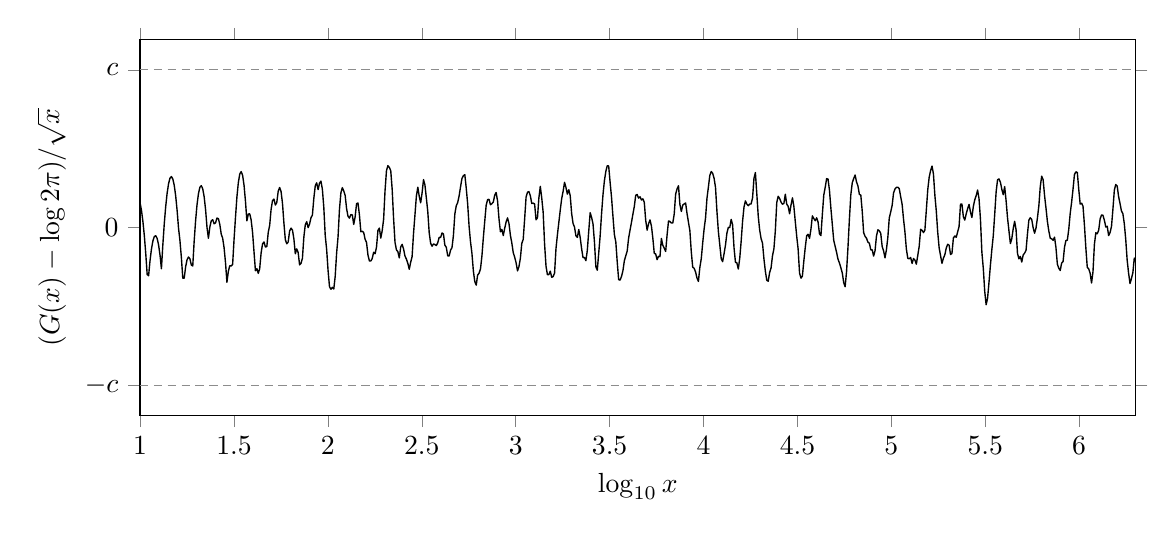
\begin{tikzpicture}
\begin{axis}[width=5.6in,height=2.5in,xmin=1,xmax=6.3,ymin=-0.055,ymax=0.055,
xlabel={$\log_{10}x$},ylabel={$(G(x)-\log2\pi)/\sqrt x$},
ytick={-0.0462,0,0.0462},yticklabels={$-c$,$0$,$c$},
scaled y ticks=false,axis background/.style={fill=white},tick align=outside,
every axis plot/.append style={line join=round}]
\addplot[black!45,densely dashed,domain=1:6.3,samples=2]{0.04619};
\addplot[black!45,densely dashed,domain=1:6.3,samples=2]{-0.04619};
\addplot[black,line width=0.5pt] coordinates {(1.0000,0.00725)(1.0076,0.00501)(1.0152,0.00179)(1.0228,-0.00241)(1.0303,-0.00759)(1.0379,-0.01378)(1.0455,-0.01413)(1.0531,-0.00972)(1.0607,-0.00633)(1.0683,-0.00397)(1.0758,-0.00266)(1.0834,-0.00241)(1.0910,-0.00321)(1.0986,-0.00509)(1.1062,-0.00804)(1.1138,-0.01209)(1.1213,-0.00512)(1.1289,0.00105)(1.1365,0.00610)(1.1441,0.01002)(1.1517,0.01280)(1.1593,0.01444)(1.1668,0.01492)(1.1744,0.01423)(1.1820,0.01236)(1.1896,0.00931)(1.1972,0.00506)(1.2048,-0.00015)(1.2123,-0.00381)(1.2199,-0.00870)(1.2275,-0.01483)(1.2351,-0.01486)(1.2427,-0.01151)(1.2503,-0.00944)(1.2578,-0.00865)(1.2654,-0.00917)(1.2730,-0.01099)(1.2806,-0.01126)(1.2882,-0.00395)(1.2958,0.00203)(1.3033,0.00665)(1.3109,0.00990)(1.3185,0.01178)(1.3261,0.01226)(1.3337,0.01134)(1.3413,0.00901)(1.3489,0.00525)(1.3564,0.00005)(1.3640,-0.00316)(1.3716,0.00013)(1.3792,0.00195)(1.3868,0.00227)(1.3944,0.00109)(1.4019,0.00136)(1.4095,0.00275)(1.4171,0.00259)(1.4247,0.00088)(1.4323,-0.00197)(1.4399,-0.00315)(1.4474,-0.00593)(1.4550,-0.01032)(1.4626,-0.01604)(1.4702,-0.01279)(1.4778,-0.01120)(1.4854,-0.01128)(1.4929,-0.01080)(1.5005,-0.00350)(1.5081,0.00293)(1.5157,0.00892)(1.5233,0.01317)(1.5309,0.01566)(1.5384,0.01638)(1.5460,0.01530)(1.5536,0.01241)(1.5612,0.00771)(1.5688,0.00195)(1.5764,0.00392)(1.5839,0.00401)(1.5915,0.00221)(1.5991,-0.00149)(1.6067,-0.00711)(1.6143,-0.01267)(1.6219,-0.01207)(1.6294,-0.01343)(1.6370,-0.01208)(1.6446,-0.00743)(1.6522,-0.00481)(1.6598,-0.00423)(1.6674,-0.00571)(1.6750,-0.00558)(1.6825,-0.00143)(1.6901,0.00060)(1.6977,0.00530)(1.7053,0.00790)(1.7129,0.00833)(1.7205,0.00657)(1.7280,0.00732)(1.7356,0.01065)(1.7432,0.01172)(1.7508,0.01053)(1.7584,0.00704)(1.7660,0.00125)(1.7735,-0.00358)(1.7811,-0.00478)(1.7887,-0.00425)(1.7963,-0.00102)(1.8039,-0.00020)(1.8115,-0.00076)(1.8190,-0.00332)(1.8266,-0.00770)(1.8342,-0.00626)(1.8418,-0.00734)(1.8494,-0.01096)(1.8570,-0.01050)(1.8645,-0.00903)(1.8721,-0.00281)(1.8797,0.00078)(1.8873,0.00171)(1.8949,-0.00004)(1.9025,0.00099)(1.9100,0.00284)(1.9176,0.00364)(1.9252,0.00851)(1.9328,0.01221)(1.9404,0.01308)(1.9480,0.01110)(1.9556,0.01301)(1.9631,0.01358)(1.9707,0.01122)(1.9783,0.00592)(1.9859,-0.00236)(1.9935,-0.00647)(2.0011,-0.01266)(2.0086,-0.01734)(2.0162,-0.01809)(2.0238,-0.01753)(2.0314,-0.01803)(2.0390,-0.01428)(2.0466,-0.00747)(2.0541,-0.00280)(2.0617,0.00531)(2.0693,0.01014)(2.0769,0.01167)(2.0845,0.01072)(2.0921,0.00937)(2.0996,0.00553)(2.1072,0.00328)(2.1148,0.00275)(2.1224,0.00378)(2.1300,0.00370)(2.1376,0.00090)(2.1451,0.00311)(2.1527,0.00696)(2.1603,0.00719)(2.1679,0.00374)(2.1755,-0.00124)(2.1831,-0.00111)(2.1906,-0.00146)(2.1982,-0.00345)(2.2058,-0.00438)(2.2134,-0.00807)(2.2210,-0.00980)(2.2286,-0.00982)(2.2361,-0.00910)(2.2437,-0.00724)(2.2513,-0.00771)(2.2589,-0.00577)(2.2665,-0.00090)(2.2741,-0.00018)(2.2817,-0.00310)(2.2892,-0.00093)(2.2968,0.00243)(2.3044,0.01082)(2.3120,0.01665)(2.3196,0.01811)(2.3272,0.01760)(2.3347,0.01665)(2.3423,0.01122)(2.3499,0.00259)(2.3575,-0.00439)(2.3651,-0.00657)(2.3727,-0.00709)(2.3802,-0.00892)(2.3878,-0.00570)(2.3954,-0.00494)(2.4030,-0.00632)(2.4106,-0.00838)(2.4182,-0.00927)(2.4257,-0.01052)(2.4333,-0.01224)(2.4409,-0.01017)(2.4485,-0.00849)(2.4561,-0.00168)(2.4637,0.00375)(2.4712,0.00917)(2.4788,0.01180)(2.4864,0.00914)(2.4940,0.00723)(2.5016,0.01014)(2.5092,0.01403)(2.5167,0.01245)(2.5243,0.00864)(2.5319,0.00465)(2.5395,-0.00154)(2.5471,-0.00463)(2.5547,-0.00549)(2.5622,-0.00483)(2.5698,-0.00499)(2.5774,-0.00529)(2.5850,-0.00447)(2.5926,-0.00289)(2.6002,-0.00294)(2.6078,-0.00161)(2.6153,-0.00189)(2.6229,-0.00517)(2.6305,-0.00581)(2.6381,-0.00832)(2.6457,-0.00835)(2.6533,-0.00663)(2.6608,-0.00592)(2.6684,-0.00237)(2.6760,0.00397)(2.6836,0.00638)(2.6912,0.00731)(2.6988,0.00927)(2.7063,0.01190)(2.7139,0.01436)(2.7215,0.01517)(2.7291,0.01548)(2.7367,0.01151)(2.7443,0.00687)(2.7518,0.00038)(2.7594,-0.00419)(2.7670,-0.00758)(2.7746,-0.01273)(2.7822,-0.01585)(2.7898,-0.01689)(2.7973,-0.01395)(2.8049,-0.01339)(2.8125,-0.01215)(2.8201,-0.00839)(2.8277,-0.00301)(2.8353,0.00190)(2.8428,0.00650)(2.8504,0.00816)(2.8580,0.00825)(2.8656,0.00666)(2.8732,0.00698)(2.8808,0.00745)(2.8883,0.00946)(2.8959,0.01026)(2.9035,0.00776)(2.9111,0.00249)(2.9187,-0.00127)(2.9263,-0.00057)(2.9339,-0.00237)(2.9414,-0.00023)(2.9490,0.00161)(2.9566,0.00282)(2.9642,0.00116)(2.9718,-0.00228)(2.9794,-0.00456)(2.9869,-0.00737)(2.9945,-0.00868)(3.0021,-0.01033)(3.0097,-0.01272)(3.0173,-0.01148)(3.0249,-0.00902)(3.0324,-0.00468)(3.0400,-0.00347)(3.0476,0.00246)(3.0552,0.00890)(3.0628,0.01033)(3.0704,0.01052)(3.0779,0.00931)(3.0855,0.00705)(3.0931,0.00714)(3.1007,0.00689)(3.1083,0.00225)(3.1159,0.00286)(3.1234,0.00866)(3.1310,0.01205)(3.1386,0.00868)(3.1462,0.00445)(3.1538,-0.00485)(3.1614,-0.01136)(3.1689,-0.01383)(3.1765,-0.01379)(3.1841,-0.01280)(3.1917,-0.01460)(3.1993,-0.01437)(3.2069,-0.01337)(3.2145,-0.00618)(3.2220,-0.00219)(3.2296,0.00147)(3.2372,0.00509)(3.2448,0.00845)(3.2524,0.01058)(3.2600,0.01323)(3.2675,0.01175)(3.2751,0.00978)(3.2827,0.01106)(3.2903,0.00929)(3.2979,0.00409)(3.3055,0.00117)(3.3130,0.00015)(3.3206,-0.00243)(3.3282,-0.00290)(3.3358,-0.00058)(3.3434,-0.00295)(3.3510,-0.00624)(3.3585,-0.00883)(3.3661,-0.00878)(3.3737,-0.00970)(3.3813,-0.00670)(3.3889,-0.00106)(3.3965,0.00434)(3.4040,0.00296)(3.4116,0.00108)(3.4192,-0.00417)(3.4268,-0.01150)(3.4344,-0.01251)(3.4420,-0.00753)(3.4495,-0.00256)(3.4571,0.00398)(3.4647,0.00959)(3.4723,0.01370)(3.4799,0.01643)(3.4875,0.01808)(3.4950,0.01803)(3.5026,0.01328)(3.5102,0.00885)(3.5178,0.00325)(3.5254,-0.00208)(3.5330,-0.00425)(3.5406,-0.01014)(3.5481,-0.01528)(3.5557,-0.01542)(3.5633,-0.01435)(3.5709,-0.01265)(3.5785,-0.00974)(3.5861,-0.00829)(3.5936,-0.00690)(3.6012,-0.00310)(3.6088,-0.00074)(3.6164,0.00149)(3.6240,0.00391)(3.6316,0.00620)(3.6391,0.00947)(3.6467,0.00965)(3.6543,0.00860)(3.6619,0.00901)(3.6695,0.00806)(3.6771,0.00840)(3.6846,0.00739)(3.6922,0.00206)(3.6998,-0.00078)(3.7074,0.00109)(3.7150,0.00223)(3.7226,0.00044)(3.7301,-0.00310)(3.7377,-0.00756)(3.7453,-0.00774)(3.7529,-0.00942)(3.7605,-0.00841)(3.7681,-0.00855)(3.7756,-0.00320)(3.7832,-0.00520)(3.7908,-0.00605)(3.7984,-0.00702)(3.8060,-0.00219)(3.8136,0.00190)(3.8211,0.00178)(3.8287,0.00130)(3.8363,0.00130)(3.8439,0.00389)(3.8515,0.00976)(3.8591,0.01130)(3.8667,0.01223)(3.8742,0.00677)(3.8818,0.00470)(3.8894,0.00654)(3.8970,0.00691)(3.9046,0.00718)(3.9122,0.00410)(3.9197,0.00156)(3.9273,-0.00093)(3.9349,-0.00715)(3.9425,-0.01164)(3.9501,-0.01196)(3.9577,-0.01305)(3.9652,-0.01480)(3.9728,-0.01579)(3.9804,-0.01171)(3.9880,-0.00917)(3.9956,-0.00452)(4.0032,-0.00040)(4.0107,0.00276)(4.0183,0.00852)(4.0259,0.01184)(4.0335,0.01526)(4.0411,0.01639)(4.0487,0.01589)(4.0562,0.01443)(4.0638,0.01176)(4.0714,0.00478)(4.0790,-0.00114)(4.0866,-0.00509)(4.0942,-0.00913)(4.1017,-0.01001)(4.1093,-0.00769)(4.1169,-0.00516)(4.1245,-0.00165)(4.1321,0.00006)(4.1397,-0.00003)(4.1472,0.00237)(4.1548,0.00081)(4.1624,-0.00596)(4.1700,-0.01017)(4.1776,-0.01039)(4.1852,-0.01217)(4.1928,-0.00904)(4.2003,-0.00409)(4.2079,0.00177)(4.2155,0.00599)(4.2231,0.00780)(4.2307,0.00686)(4.2383,0.00639)(4.2458,0.00684)(4.2534,0.00693)(4.2610,0.00863)(4.2686,0.01442)(4.2762,0.01609)(4.2838,0.00975)(4.2913,0.00334)(4.2989,-0.00073)(4.3065,-0.00326)(4.3141,-0.00459)(4.3217,-0.00922)(4.3293,-0.01284)(4.3368,-0.01549)(4.3444,-0.01574)(4.3520,-0.01319)(4.3596,-0.01185)(4.3672,-0.00828)(4.3748,-0.00623)(4.3823,-0.00098)(4.3899,0.00730)(4.3975,0.00915)(4.4051,0.00851)(4.4127,0.00743)(4.4203,0.00681)(4.4278,0.00702)(4.4354,0.00974)(4.4430,0.00685)(4.4506,0.00622)(4.4582,0.00402)(4.4658,0.00658)(4.4734,0.00869)(4.4809,0.00624)(4.4885,0.00178)(4.4961,-0.00253)(4.5037,-0.00636)(4.5113,-0.01339)(4.5189,-0.01484)(4.5264,-0.01424)(4.5340,-0.00985)(4.5416,-0.00589)(4.5492,-0.00243)(4.5568,-0.00198)(4.5644,-0.00319)(4.5719,-0.00052)(4.5795,0.00339)(4.5871,0.00265)(4.5947,0.00198)(4.6023,0.00284)(4.6099,0.00156)(4.6174,-0.00187)(4.6250,-0.00238)(4.6326,0.00379)(4.6402,0.00948)(4.6478,0.01174)(4.6554,0.01431)(4.6629,0.01418)(4.6705,0.01091)(4.6781,0.00567)(4.6857,0.00088)(4.6933,-0.00381)(4.7009,-0.00553)(4.7084,-0.00728)(4.7160,-0.00930)(4.7236,-0.01039)(4.7312,-0.01179)(4.7388,-0.01332)(4.7464,-0.01619)(4.7539,-0.01735)(4.7615,-0.01292)(4.7691,-0.00580)(4.7767,0.00248)(4.7843,0.00961)(4.7919,0.01311)(4.7995,0.01433)(4.8070,0.01538)(4.8146,0.01335)(4.8222,0.01215)(4.8298,0.00969)(4.8374,0.00949)(4.8450,0.00474)(4.8525,-0.00152)(4.8601,-0.00259)(4.8677,-0.00314)(4.8753,-0.00431)(4.8829,-0.00460)(4.8905,-0.00655)(4.8980,-0.00654)(4.9056,-0.00838)(4.9132,-0.00680)(4.9208,-0.00248)(4.9284,-0.00068)(4.9360,-0.00097)(4.9435,-0.00172)(4.9511,-0.00555)(4.9587,-0.00687)(4.9663,-0.00889)(4.9739,-0.00649)(4.9815,-0.00277)(4.9890,0.00282)(4.9966,0.00456)(5.0042,0.00645)(5.0118,0.01013)(5.0194,0.01128)(5.0270,0.01178)(5.0345,0.01179)(5.0421,0.01136)(5.0497,0.00902)(5.0573,0.00683)(5.0649,0.00243)(5.0725,-0.00139)(5.0800,-0.00634)(5.0876,-0.00904)(5.0952,-0.00916)(5.1028,-0.00879)(5.1104,-0.01055)(5.1180,-0.00910)(5.1256,-0.00957)(5.1331,-0.01074)(5.1407,-0.00819)(5.1483,-0.00550)(5.1559,-0.00053)(5.1635,-0.00086)(5.1711,-0.00150)(5.1786,-0.00076)(5.1862,0.00505)(5.1938,0.01102)(5.2014,0.01472)(5.2090,0.01668)(5.2166,0.01800)(5.2241,0.01568)(5.2317,0.00946)(5.2393,0.00480)(5.2469,-0.00142)(5.2545,-0.00597)(5.2621,-0.00830)(5.2696,-0.01052)(5.2772,-0.00898)(5.2848,-0.00799)(5.2924,-0.00600)(5.3000,-0.00491)(5.3076,-0.00519)(5.3151,-0.00793)(5.3227,-0.00759)(5.3303,-0.00306)(5.3379,-0.00250)(5.3455,-0.00286)(5.3531,-0.00128)(5.3606,0.00030)(5.3682,0.00682)(5.3758,0.00686)(5.3834,0.00316)(5.3910,0.00217)(5.3986,0.00400)(5.4061,0.00548)(5.4137,0.00676)(5.4213,0.00454)(5.4289,0.00292)(5.4365,0.00616)(5.4441,0.00809)(5.4517,0.00934)(5.4592,0.01096)(5.4668,0.00845)(5.4744,0.00243)(5.4820,-0.00726)(5.4896,-0.01199)(5.4972,-0.01876)(5.5047,-0.02264)(5.5123,-0.02069)(5.5199,-0.01608)(5.5275,-0.01102)(5.5351,-0.00647)(5.5427,-0.00243)(5.5502,0.00376)(5.5578,0.01039)(5.5654,0.01396)(5.5730,0.01424)(5.5806,0.01327)(5.5882,0.01119)(5.5957,0.00959)(5.6033,0.01198)(5.6109,0.00785)(5.6185,0.00284)(5.6261,-0.00097)(5.6337,-0.00472)(5.6412,-0.00331)(5.6488,-0.00036)(5.6564,0.00180)(5.6640,-0.00065)(5.6716,-0.00760)(5.6792,-0.00919)(5.6867,-0.00848)(5.6943,-0.01012)(5.7019,-0.00806)(5.7095,-0.00750)(5.7171,-0.00670)(5.7247,-0.00189)(5.7322,0.00217)(5.7398,0.00285)(5.7474,0.00235)(5.7550,-0.00008)(5.7626,-0.00167)(5.7702,-0.00016)(5.7778,0.00282)(5.7853,0.00631)(5.7929,0.01199)(5.8005,0.01504)(5.8081,0.01397)(5.8157,0.00938)(5.8233,0.00568)(5.8308,0.00178)(5.8384,-0.00104)(5.8460,-0.00315)(5.8536,-0.00332)(5.8612,-0.00376)(5.8688,-0.00284)(5.8763,-0.00584)(5.8839,-0.01076)(5.8915,-0.01192)(5.8991,-0.01260)(5.9067,-0.01043)(5.9143,-0.00999)(5.9218,-0.00583)(5.9294,-0.00382)(5.9370,-0.00373)(5.9446,-0.00051)(5.9522,0.00409)(5.9598,0.00741)(5.9673,0.01124)(5.9749,0.01552)(5.9825,0.01631)(5.9901,0.01611)(5.9977,0.01123)(6.0053,0.00686)(6.0128,0.00712)(6.0204,0.00627)(6.0280,0.00073)(6.0356,-0.00604)(6.0432,-0.01172)(6.0508,-0.01213)(6.0584,-0.01341)(6.0659,-0.01626)(6.0735,-0.01301)(6.0811,-0.00496)(6.0887,-0.00153)(6.0963,-0.00182)(6.1039,-0.00082)(6.1114,0.00247)(6.1190,0.00368)(6.1266,0.00357)(6.1342,0.00212)(6.1418,0.00012)(6.1494,0.00035)(6.1569,-0.00238)(6.1645,-0.00147)(6.1721,0.00031)(6.1797,0.00537)(6.1873,0.01097)(6.1949,0.01259)(6.2024,0.01213)(6.2100,0.00904)(6.2176,0.00699)(6.2252,0.00482)(6.2328,0.00404)(6.2404,0.00109)(6.2479,-0.00350)(6.2555,-0.00956)(6.2631,-0.01337)(6.2707,-0.01642)(6.2783,-0.01496)(6.2859,-0.01325)(6.2934,-0.00897)(6.3010,-0.00997)};
\end{axis}
\end{tikzpicture}
\caption{The quantity $(G(x)-\log2\pi)/\sqrt x$ for $10\le x\le2\cdot10^6$, computed from \eqref{G}. The dashed lines are at $\pm c$ with $c=2+\gamma-\log4\pi\approx0.0462$. The Riemann hypothesis holds exactly when $G(x)\le C_\varepsilon x^{1/2+\varepsilon}$ for every $\varepsilon>0$, and by Corollary~\ref{corA} it is enough to know this on a sequence of windows $Y\le x\le Y^\lambda$.}\label{fig}
\end{figure}

\section{Zeros against poles}\label{sec:zp}

The bound \eqref{eq:intro-window} has the shape of an upper bound for the number of points of a curve over a finite field. This section gives the proof of that bound by the method of Stepanov, proves the inequality that replaces its last step over the integers, and runs the replacement on an example in which it produces a sum over primes.

\subsection{The model over a finite field}\label{sec:ff}

Alp\"oge's note \cite{note} calls the route a descendant of Stepanov's proof \cite{stepanov} of the Riemann hypothesis for curves over finite fields. We give the version of Bombieri \cite{bombieri} in full, because each of its five steps has a counterpart in the later sections.

Let $q$ be a power of a prime $p$, and let $X$ be a smooth projective geometrically irreducible curve of genus $g$ over $\mathbb F_q$. Fix a rational point $P_0$ of $X$. For an integer $k\ge0$ let $L(k)$ be the space of rational functions on $X$ that are regular away from $P_0$ and have a pole of order at most $k$ at $P_0$. The Riemann--Roch theorem gives $k+1-g\le\dim L(k)\le k+1$, with $\dim L(k)=k+1-g$ when $k\ge2g-1$.

\begin{theorem}[Stepanov, Bombieri]\label{stepanov}
Let $X$ be a smooth projective geometrically irreducible curve of genus $g$ over $\mathbb F_q$, and suppose that $q=q_0^2$ is a square with $q_0>(g+1)^2$. Then the number $N$ of $\mathbb F_q$-rational points of $X$ satisfies $N\le q+(2g+1)\sqrt q$.
\end{theorem}
\begin{proof}
If $N=0$ the bound holds, so we fix a rational point $P_0$. Let $M$ be a power of $p$ with $M\le q$, and let $\ell,n$ be positive integers with $\ell M<q$.

\emph{Step 1, the auxiliary space.} Choose a basis $a_1,\dots,a_r$ of $L(\ell)$ with pairwise distinct pole orders at $P_0$, and let $V$ be the set of functions
\[
f=\sum_{i=1}^ra_i^M\,b_i^{\,q},\qquad b_i\in L(n).
\]
Suppose $f=0$ while some $b_i\ne0$. Two nonzero terms then have equal pole order at $P_0$, so $M(\operatorname{ord}a_i-\operatorname{ord}a_j)=q(\operatorname{ord}b_j-\operatorname{ord}b_i)$ for some $i\ne j$. The left side is a nonzero integer of absolute value at most $\ell M<q$ and the right side is a multiple of $q$, which is impossible. Hence the $b_i$ are determined by $f$, and
\[
\dim V=\dim L(\ell)\dim L(n)\ge(\ell+1-g)(n+1-g).
\]

\emph{Step 2, the comparison map.} By Step 1 the map $\delta\colon V\to L(\ell M+n)$, $\delta(f)=\sum_ia_i^Mb_i$, is well defined and $\mathbb F_q$-linear. Its kernel is nonzero as soon as
\begin{equation}\label{kernel}
(\ell+1-g)(n+1-g)>\ell M+n+1-g .
\end{equation}

\emph{Step 3, multiplicity.} Let $f\ne0$ with $\delta(f)=0$ and let $P\ne P_0$ be a rational point. Since $b_i(P)^q=b_i(P)$, we get $f(P)=\delta(f)(P)=0$. Moreover $f=\big(\sum_ia_i\,b_i^{\,q/M}\big)^M$, so $f$ vanishes to order at least $M$ at $P$.

\emph{Step 4, zeros against poles.} A nonzero rational function has as many zeros as poles. The poles of $f$ lie at $P_0$ and number at most $\ell M+nq$, hence
\begin{equation}\label{count}
M(N-1)\le\ell M+nq,\qquad N-1\le\ell+\frac{nq}M .
\end{equation}

\emph{Step 5, the parameters.} Take $n=M+2g$ and $\ell=\lfloor gM/(g+1)\rfloor+g+1$. Then $\ell(g+1)>g(M+g+1)$, which is \eqref{kernel}, and \eqref{count} reads $N-1\le q+\ell+2gq/M$. Take $M=q_0$. The hypothesis $q_0>(g+1)^2$ gives $\ell<q_0$, so $\ell M<q$, and $N-1<q+q_0+2gq_0$.
\end{proof}

Before the final choice the error is $\ell+2gq/M$ with $\ell$ close to $M$. With $M=1$ the bound \eqref{count} reads $N-1\le(2g+1)q+g+1$, whose main term is already too large, and the two contributions balance at $M=\sqrt q$. Figure~\ref{figell} compares the theorem with computed point counts.

\begin{figure}[htbp]
\centering
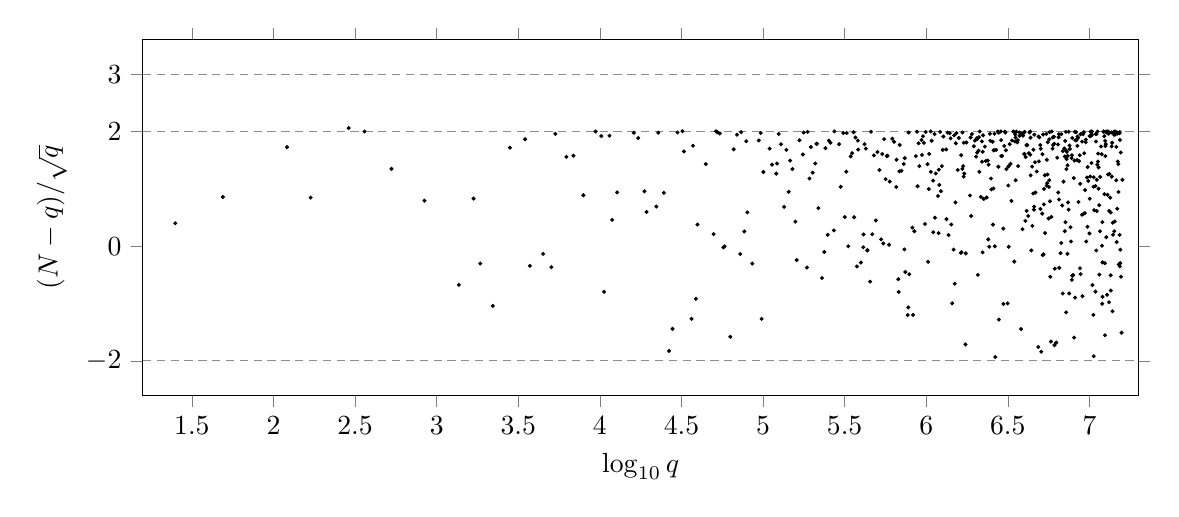
\begin{tikzpicture}
\begin{axis}[width=5.6in,height=2.4in,xmin=1.2,xmax=7.3,ymin=-2.6,ymax=3.6,
xlabel={$\log_{10}q$},ylabel={$(N-q)/\sqrt q$},ytick={-2,0,2,3},
axis background/.style={fill=white},tick align=outside]
\addplot[black!45,densely dashed,domain=1.2:7.3,samples=2]{3};
\addplot[black!45,densely dashed,domain=1.2:7.3,samples=2]{2};
\addplot[black!45,densely dashed,domain=1.2:7.3,samples=2]{-2};
\addplot[black,only marks,mark=*,mark size=0.5pt] coordinates {(1.398,0.4000)(1.690,0.8571)(2.083,1.7273)(2.228,0.8462)(2.461,2.0588)(2.558,2.0000)(2.723,1.3478)(2.925,0.7931)(3.136,-0.6757)(3.226,0.8293)(3.267,-0.3023)(3.344,-1.0426)(3.449,1.7170)(3.542,1.8644)(3.571,-0.3443)(3.652,-0.1343)(3.703,-0.3662)(3.727,1.9589)(3.795,1.5570)(3.838,1.5783)(3.899,0.8876)(3.974,2.0000)(4.009,1.9208)(4.026,-0.7961)(4.059,1.9252)(4.075,0.4587)(4.106,0.9381)(4.208,1.9764)(4.235,1.8855)(4.273,0.9562)(4.286,0.5971)(4.346,0.6913)(4.358,1.9801)(4.392,0.9299)(4.424,-1.8282)(4.445,-1.4431)(4.476,1.9827)(4.506,2.0056)(4.515,1.6519)(4.562,-1.2670)(4.571,1.7513)(4.589,-0.9188)(4.598,0.3769)(4.649,1.4313)(4.697,0.2108)(4.712,2.0044)(4.720,1.9869)(4.735,1.9657)(4.757,-0.0209)(4.764,-0.0041)(4.799,-1.5817)(4.820,1.6887)(4.840,1.9430)(4.860,-0.1375)(4.866,1.9889)(4.885,0.2563)(4.897,1.8292)(4.904,0.5901)(4.934,-0.3038)(4.974,1.8436)(4.986,1.9743)(4.991,-1.2684)(5.002,1.2934)(5.040,1.7009)(5.055,1.4214)(5.081,1.2651)(5.086,1.4413)(5.096,1.9575)(5.110,1.7772)(5.129,0.6839)(5.143,1.6783)(5.157,0.9472)(5.166,1.4909)(5.180,1.3445)(5.198,0.4282)(5.206,-0.2419)(5.223,1.8460)(5.244,1.5990)(5.249,1.9810)(5.269,-0.3735)(5.273,1.9931)(5.285,1.1800)(5.293,1.7291)(5.304,1.2806)(5.320,1.4420)(5.327,1.7852)(5.331,1.7862)(5.339,0.6638)(5.361,-0.5553)(5.375,-0.1006)(5.382,1.7088)(5.396,0.1984)(5.403,1.8410)(5.413,1.8055)(5.434,0.2745)(5.437,2.0019)(5.466,1.7782)(5.476,1.0347)(5.492,1.9731)(5.501,0.5080)(5.510,1.2988)(5.513,1.9737)(5.522,-0.0017)(5.537,1.5656)(5.546,1.6223)(5.555,1.9866)(5.558,0.5042)(5.566,1.8962)(5.575,-0.3540)(5.581,1.8395)(5.583,1.6850)(5.600,-0.2868)(5.614,-0.0203)(5.616,0.2037)(5.622,1.7790)(5.630,1.7014)(5.638,-0.0759)(5.640,-0.0696)(5.656,-0.6196)(5.661,1.9956)(5.669,0.2079)(5.679,1.5832)(5.691,0.4479)(5.701,1.6403)(5.713,1.3282)(5.723,0.1183)(5.730,1.6071)(5.737,0.0474)(5.742,1.8668)(5.751,1.1691)(5.758,1.5733)(5.763,1.5756)(5.772,0.0234)(5.776,1.1268)(5.792,1.8742)(5.803,1.8206)(5.816,1.0321)(5.818,1.5080)(5.829,-0.5761)(5.831,-0.7983)(5.835,1.3047)(5.837,1.7648)(5.848,1.3147)(5.862,1.4338)(5.866,-0.0572)(5.868,1.5355)(5.872,-0.4508)(5.886,-1.2018)(5.890,-1.0681)(5.892,1.9830)(5.896,-0.4893)(5.915,0.3241)(5.919,-1.1998)(5.927,0.2601)(5.936,1.5705)(5.943,1.9968)(5.947,1.0446)(5.953,1.7941)(5.958,1.3966)(5.971,1.8521)(5.974,1.5891)(5.980,1.9181)(5.985,1.8016)(5.992,0.3865)(5.997,1.9920)(6.008,1.4301)(6.011,-0.2734)(6.016,0.9961)(6.018,1.6092)(6.027,2.0010)(6.028,1.2953)(6.033,1.8383)(6.042,1.1430)(6.043,0.2417)(6.051,1.9548)(6.053,0.4958)(6.058,1.2675)(6.072,0.8740)(6.076,0.2264)(6.077,1.3339)(6.080,1.0675)(6.085,1.9927)(6.090,0.9585)(6.096,1.3957)(6.101,1.6794)(6.105,1.9123)(6.122,1.6872)(6.124,0.4709)(6.131,1.9794)(6.137,0.1939)(6.144,1.9704)(6.149,1.8795)(6.153,0.3780)(6.159,-0.9967)(6.168,-0.0602)(6.171,1.9343)(6.175,-0.6558)(6.179,0.7632)(6.181,1.7929)(6.185,1.9717)(6.193,1.3275)(6.200,1.8864)(6.212,-0.1167)(6.214,1.5872)(6.216,-0.1068)(6.221,1.3483)(6.222,1.9814)(6.226,1.3963)(6.229,1.2137)(6.230,1.8043)(6.233,1.2655)(6.240,-1.7142)(6.242,-0.1257)(6.246,1.8078)(6.268,0.8832)(6.272,1.8954)(6.275,0.5259)(6.280,1.9544)(6.292,1.7427)(6.298,1.8410)(6.306,1.5615)(6.309,1.8823)(6.310,1.8635)(6.312,1.6315)(6.316,-0.5010)(6.321,1.6662)(6.323,1.9014)(6.325,1.2959)(6.328,2.0000)(6.335,0.8579)(6.341,1.8278)(6.342,1.4720)(6.345,-0.1083)(6.346,1.6454)(6.348,1.9337)(6.352,0.8239)(6.359,1.7359)(6.365,1.4859)(6.370,0.8485)(6.377,1.4925)(6.380,0.1181)(6.382,1.4211)(6.386,-0.0109)(6.390,1.9598)(6.392,1.8377)(6.397,1.1799)(6.399,0.9899)(6.407,1.8197)(6.409,0.3760)(6.412,1.0050)(6.413,1.6718)(6.415,1.6727)(6.418,1.9611)(6.420,-0.0037)(6.423,-1.9330)(6.428,1.6775)(6.439,2.0000)(6.442,1.3848)(6.444,1.9790)(6.445,-1.2804)(6.457,2.0000)(6.459,1.8497)(6.460,1.5715)(6.465,1.5740)(6.472,0.3062)(6.473,-1.0081)(6.478,1.7461)(6.482,1.9983)(6.485,1.9800)(6.488,1.6720)(6.491,1.3434)(6.499,-0.9983)(6.502,1.0578)(6.504,1.3912)(6.505,-0.0117)(6.511,1.7785)(6.516,1.4351)(6.522,0.7888)(6.525,1.8427)(6.533,2.0000)(6.539,-0.2697)(6.542,1.9871)(6.544,1.8274)(6.545,1.9471)(6.547,1.8961)(6.548,1.1490)(6.552,1.9984)(6.558,1.8106)(6.561,1.8490)(6.563,1.3962)(6.572,1.9259)(6.572,1.9819)(6.580,1.9677)(6.581,-1.4459)(6.590,0.2955)(6.593,1.9277)(6.596,1.9683)(6.599,1.9824)(6.601,1.6079)(6.602,1.6083)(6.603,1.9925)(6.607,0.4411)(6.609,1.5543)(6.614,1.7617)(6.615,0.6161)(6.619,1.7631)(6.625,0.5270)(6.629,1.6205)(6.632,1.9831)(6.637,1.5963)(6.637,1.9986)(6.639,1.8927)(6.640,1.2346)(6.644,-0.0748)(6.649,1.3865)(6.650,0.3531)(6.656,0.9183)(6.657,1.6832)(6.660,0.6359)(6.661,0.6885)(6.662,1.9440)(6.666,1.4635)(6.669,0.9343)(6.677,1.3024)(6.686,-1.7585)(6.688,1.9116)(6.690,1.4781)(6.693,1.8991)(6.699,1.7640)(6.700,0.6494)(6.702,1.6991)(6.705,-1.8418)(6.711,0.5673)(6.712,1.6038)(6.713,-0.1553)(6.716,1.9474)(6.719,-0.1421)(6.721,0.7287)(6.722,0.9974)(6.727,1.2365)(6.728,0.2280)(6.736,1.9576)(6.738,1.0560)(6.739,1.5066)(6.741,1.0988)(6.743,1.2501)(6.745,1.8133)(6.750,0.4821)(6.752,1.0311)(6.754,1.1499)(6.754,1.8645)(6.756,1.9900)(6.758,0.7819)(6.760,-0.5356)(6.764,-1.6645)(6.767,0.5110)(6.769,2.0000)(6.774,1.7013)(6.775,1.8955)(6.777,1.7650)(6.782,1.9089)(6.784,1.7860)(6.786,-1.7262)(6.788,-0.3932)(6.797,-1.6816)(6.803,1.5418)(6.807,1.7728)(6.809,0.9354)(6.811,1.8997)(6.813,0.8137)(6.813,1.9530)(6.815,-0.3790)(6.823,-0.1229)(6.827,0.0548)(6.828,1.9537)(6.833,0.7110)(6.836,-0.8258)(6.837,1.6570)(6.841,1.1253)(6.846,1.7042)(6.849,1.5653)(6.849,0.2614)(6.851,1.8348)(6.853,0.4186)(6.855,1.9944)(6.857,-1.1543)(6.859,1.3439)(6.859,1.6657)(6.860,1.5191)(6.862,1.6443)(6.865,-0.1334)(6.866,1.4102)(6.867,1.5743)(6.869,0.7631)(6.872,0.6369)(6.873,1.9945)(6.876,-0.8249)(6.878,1.7545)(6.880,1.6949)(6.884,0.3292)(6.887,0.0814)(6.891,1.5357)(6.892,-0.5883)(6.893,1.5871)(6.895,1.8847)(6.895,-0.5169)(6.900,-0.5027)(6.904,1.1871)(6.906,-1.5953)(6.908,1.4924)(6.910,1.9947)(6.912,-0.8981)(6.913,1.8462)(6.918,1.9878)(6.921,1.8476)(6.924,1.5019)(6.926,1.7492)(6.927,1.9123)(6.930,1.8893)(6.933,0.7704)(6.936,1.4828)(6.941,1.5855)(6.942,-0.3859)(6.943,1.0877)(6.945,1.9518)(6.946,-0.4891)(6.954,0.5478)(6.955,1.8241)(6.957,-0.8721)(6.960,1.9526)(6.961,1.9735)(6.965,0.5660)(6.966,1.9885)(6.968,1.6212)(6.972,0.5773)(6.973,0.9778)(6.977,1.8133)(6.978,1.8573)(6.980,0.0809)(6.985,1.1962)(6.988,0.3382)(6.989,1.3800)(6.993,1.1383)(7.000,0.2219)(7.001,1.9195)(7.002,0.8261)(7.005,1.2144)(7.007,1.9953)(7.008,1.9201)(7.011,1.9975)(7.013,1.4506)(7.015,1.9991)(7.016,1.9395)(7.018,-0.6782)(7.024,-1.1999)(7.025,1.0363)(7.026,-1.9202)(7.026,1.2022)(7.029,0.6279)(7.037,-0.7933)(7.037,1.0503)(7.039,1.9568)(7.040,1.8264)(7.042,-0.0753)(7.043,1.9570)(7.045,0.6113)(7.045,1.1570)(7.048,1.4212)(7.049,1.9991)(7.052,1.4751)(7.053,1.6147)(7.056,1.0024)(7.056,1.3730)(7.060,0.7150)(7.061,-0.4957)(7.065,0.2601)(7.066,1.2080)(7.071,1.7381)(7.075,1.6034)(7.077,0.0075)(7.078,-1.0058)(7.079,0.4190)(7.080,-0.8840)(7.080,-0.2831)(7.086,1.9977)(7.088,1.9957)(7.091,1.9180)(7.092,0.9073)(7.095,-0.2963)(7.095,-1.5543)(7.096,1.8372)(7.098,1.5705)(7.098,1.7461)(7.100,1.7793)(7.102,1.9958)(7.103,0.1568)(7.106,1.9824)(7.108,-0.8484)(7.108,2.0000)(7.111,0.8956)(7.114,1.2506)(7.116,1.9958)(7.117,1.9605)(7.118,1.9727)(7.120,-0.9785)(7.121,0.6142)(7.123,1.2580)(7.127,0.8456)(7.130,0.5881)(7.130,-0.5088)(7.131,-0.7740)(7.134,1.9829)(7.136,1.7403)(7.137,1.2124)(7.139,1.8037)(7.141,-1.1361)(7.143,0.4094)(7.144,0.1990)(7.146,1.9786)(7.151,1.9404)(7.152,2.0003)(7.152,0.2595)(7.155,0.4313)(7.158,1.9908)(7.159,1.9486)(7.160,1.9961)(7.164,1.1500)(7.165,1.7324)(7.167,0.0707)(7.170,0.6527)(7.171,1.9629)(7.172,1.9792)(7.174,1.4761)(7.177,1.4305)(7.178,0.9449)(7.180,-0.3204)(7.184,1.9693)(7.185,0.1961)(7.186,-0.3526)(7.186,1.9911)(7.187,1.8534)(7.189,-0.0613)(7.189,-0.2956)(7.192,1.6340)(7.193,-0.5333)(7.197,-1.5097)(7.202,1.1569)};
\end{axis}
\end{tikzpicture}
\caption{The curve $y^2=x^3+x+1$, of genus one, over the fields $\mathbb F_q$ with $q=p^2$ and $5\le p<4000$, $p\ne31$. Each dot is $(N-q)/\sqrt q$ for the computed number $N$ of rational points. Theorem~\ref{stepanov} proves that the dots lie below the top dashed line at $2g+1=3$. The lines at $\pm2$ are the sharp bounds of Hasse and Weil, up to $1/\sqrt q$.}\label{figell}
\end{figure}

\subsection{The slope inequality over the integers}\label{sec:slopes}

Step 4 has an arithmetic counterpart in the slope inequality of Bost \cite{bost}, built on the slopes of lattices studied by Stuhler \cite{stuhler} and Grayson \cite{grayson}. We prove it for lattices over $\mathbb Z$, where the proof takes one page.

A Euclidean lattice $\bar E=(E,\|\cdot\|)$ is a free $\mathbb Z$-module $E$ of finite rank $n\ge1$ with a Euclidean norm on $E\otimes\mathbb R$. For a basis $e_1,\dots,e_n$ of $E$ put
\begin{gather*}
\operatorname{covol}(\bar E)=\|e_1\wedge\dots\wedge e_n\|=\det\big(\langle e_i,e_j\rangle\big)^{1/2},\\
\widehat{\deg}\,\bar E=-\log\operatorname{covol}(\bar E),\qquad\hat\mu(\bar E)=\frac{\widehat{\deg}\,\bar E}{n}.
\end{gather*}
A sublattice of $E$ has the restricted norm, and a quotient $E/E'$ by a sublattice $E'$ with $E/E'$ free has the quotient norm. The Gram--Schmidt process gives $\operatorname{covol}(\bar E)=\operatorname{covol}(\bar E')\operatorname{covol}(\overline{E/E'})$, so that
\begin{equation}\label{add}
\widehat{\deg}\,\bar E=\widehat{\deg}\,\bar E'+\widehat{\deg}\,\overline{E/E'} .
\end{equation}
The maximal slope $\hat\mu_{\max}(\bar E)$ is the supremum of $\hat\mu(\bar E')$ over the nonzero sublattices $E'$ of $E$.

\begin{lemma}\label{mumax}
For every Euclidean lattice $\bar E$ the maximal slope $\hat\mu_{\max}(\bar E)$ is finite.
\end{lemma}
\begin{proof}
Let $E'$ be a sublattice of rank $k$ with basis $v_1,\dots,v_k$. The vector $v_1\wedge\dots\wedge v_k$ is a nonzero element of the lattice $\Lambda^kE$ in the Euclidean space $\Lambda^k(E\otimes\mathbb R)$, so its norm is at least the length $m_k>0$ of a shortest nonzero vector of that lattice. Hence $\hat\mu(\bar E')\le-\frac1k\log m_k$, and $k$ takes the values $1,\dots,n$.
\end{proof}

\begin{theorem}[Slope inequality over $\mathbb Z$]\label{slope}
Let $\bar E$ and $\bar F$ be Euclidean lattices, let $n$ be the rank of $E$, and let $\varphi\colon E\to F$ be an injective $\mathbb Z$-linear map. Write $\|\varphi\|$ for the operator norm of $\varphi\otimes\mathbb R$ and put $\|\Lambda^n\varphi\|=\operatorname{covol}(\overline{\varphi(E)})/\operatorname{covol}(\bar E)$, where $\varphi(E)$ has the norm of $\bar F$.
\begin{enumerate}
\item[(i)] $\widehat{\deg}\,\bar E\le n\,\hat\mu_{\max}(\bar F)+\log\|\Lambda^n\varphi\|$.
\item[(ii)] $\widehat{\deg}\,\bar E\le n\big(\hat\mu_{\max}(\bar F)+\log\|\varphi\|\big)$.
\item[(iii)] Let $F=F^0\supset F^1\supset\dots\supset F^J$ be sublattices with every $F^i/F^{i+1}$ free and with $\varphi^{-1}(F^J)=0$. Put $E^i=\varphi^{-1}(F^i)$, give $E^i/E^{i+1}$ and $F^i/F^{i+1}$ the quotient norms, and let $\varphi_i\colon E^i/E^{i+1}\to F^i/F^{i+1}$ be the map induced by $\varphi$. Then
\[
\widehat{\deg}\,\bar E\le\sum_{i=0}^{J-1}\operatorname{rk}\big(E^i/E^{i+1}\big)\Big(\hat\mu_{\max}\big(\overline{F^i/F^{i+1}}\big)+\log\|\varphi_i\|\Big).
\]
\end{enumerate}
\end{theorem}
\begin{proof}
The image $\varphi(E)$ is a sublattice of $F$ of rank $n$, so $-\log\operatorname{covol}(\overline{\varphi(E)})\le n\,\hat\mu_{\max}(\bar F)$ by the definition of the maximal slope. The left side equals $\widehat{\deg}\,\bar E-\log\|\Lambda^n\varphi\|$ by the definition of $\|\Lambda^n\varphi\|$, which is (i). The number $\|\Lambda^n\varphi\|$ is the product of the $n$ singular values of $\varphi\otimes\mathbb R$, and each singular value is at most $\|\varphi\|$, so $\|\Lambda^n\varphi\|\le\|\varphi\|^n$ and (ii) follows from (i). For (iii), each $\varphi_i$ is injective by the definition of $E^{i+1}$, hence $E^i/E^{i+1}$ is free, and $E^J=0$. Applying \eqref{add} along the chain $E=E^0\supset E^1\supset\dots\supset E^J=0$ gives $\widehat{\deg}\,\bar E=\sum_{i<J}\widehat{\deg}\,\overline{E^i/E^{i+1}}$, and (ii) applied to each $\varphi_i$ gives the claim.
\end{proof}

The parallel with Section~\ref{sec:ff} runs as follows. The lattice $E$ plays the role of the auxiliary space $V$ of Step 1, and its arithmetic degree is large when it has many elements of small norm, which is what an arithmetic Riemann--Roch theorem provides. The map $\varphi$ evaluates an auxiliary function at the points of interest, and the filtration $F^i$ in (iii) is the filtration by order of vanishing, so $\varphi_i$ records the Taylor coefficients of order $i$. Part (iii) is the count of zeros against poles. In transcendence proofs the norms $\|\varphi_i\|$ shrink as $i$ grows, by a Schwarz lemma, and this shrinking is the form that multiplicity takes over a number field. Bost's theorem \cite{bost} is the same statement for hermitian lattices over the ring of integers of a number field, with a contribution to $\log\|\varphi_i\|$ from every place. We did not write out that proof.

\subsection{Primes from an integer determinant}\label{sec:cheb}

The slope inequality produces a sum over primes in the simplest example we know, and the computation shows where such a sum enters. Let $\psi(x)=\sum_{m\le x}\Lambda(m)$, so that $\psi(N)$ is the logarithm of the least common multiple of $1,\dots,N$, and let $H_n=\big(1/(i+j+1)\big)_{0\le i,j<n}$ be the Hilbert matrix \cite{hilbert}.

\begin{proposition}\label{cheb}
For every integer $n\ge1$, with $\psi$ and $H_n$ as above, $n\,\psi(2n-1)\ge\log\big(1/\det H_n\big)$.
\end{proposition}
\begin{proof}
Let $E$ be the lattice of polynomials of degree less than $n$ with integer coefficients, with the norm of $L^2(0,1)$. In the basis $1,x,\dots,x^{n-1}$ its Gram matrix is $H_n$, so $\widehat{\deg}\,\bar E=-\tfrac12\log\det H_n$. Let $d$ be the least common multiple of $1,\dots,2n-1$ and define
\[
\varphi\colon E\to\mathbb Z^n,\qquad\varphi(P)=\Big(d\int_0^1x^jP(x)\,dx\Big)_{0\le j<n}.
\]
The matrix of $\varphi$ is $d\,H_n$, which has integer entries and nonzero determinant, so $\varphi$ is an injective map of lattices and $\operatorname{covol}(\varphi(E))=d^n\det H_n$ for the standard norm on $\mathbb Z^n$. Hence $\log\|\Lambda^n\varphi\|=n\log d+\tfrac12\log\det H_n$. Every sublattice of $\mathbb Z^n$ has a Gram determinant that is a positive integer, so $\hat\mu_{\max}(\mathbb Z^n)=0$. Theorem~\ref{slope}(i) gives $-\tfrac12\log\det H_n\le n\log d+\tfrac12\log\det H_n$, and $\log d=\psi(2n-1)$.
\end{proof}

The inequality says that the integer $d^n\det H_n$ is at least one. The classical evaluation $\det H_n=c_n^4/c_{2n}$ with $c_n=\prod_{i<n}i!$ gives $\log(1/\det H_n)=2n^2\log2-n\log2\pi+O(\log n)$, and therefore
\[
\psi(2n-1)\ge2n\log2-\log2\pi+O\Big(\frac{\log n}{n}\Big),
\]
which is Chebyshev's lower bound $\psi(N)\ge(\log2)N-O(1)$. Part (ii) of Theorem~\ref{slope}, with $\|\varphi\|^n$ in place of $\|\Lambda^n\varphi\|$, gives half of this constant. Figure~\ref{fighil} shows both sides.

\begin{figure}[htbp]
\centering
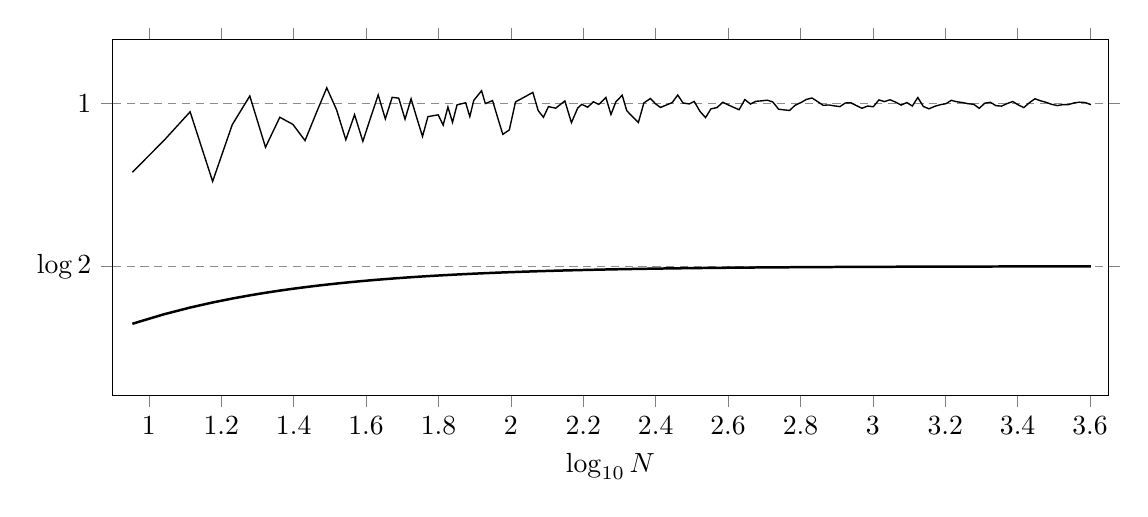
\begin{tikzpicture}
\begin{axis}[width=5.6in,height=2.4in,xmin=0.9,xmax=3.65,ymin=0.45,ymax=1.12,
xlabel={$\log_{10}N$},ytick={0.6931,1},yticklabels={$\log2$,$1$},
axis background/.style={fill=white},tick align=outside]
\addplot[black!45,densely dashed,domain=0.9:3.65,samples=2]{1};
\addplot[black!45,densely dashed,domain=0.9:3.65,samples=2]{0.6931};
\addplot[black,line width=0.5pt] coordinates {(0.9542,0.87022)(1.0414,0.92999)(1.1139,0.98422)(1.1761,0.85299)(1.2304,0.96007)(1.2788,1.01398)(1.3222,0.91741)(1.3617,0.97396)(1.3979,0.96042)(1.4314,0.92997)(1.4624,0.98195)(1.4914,1.02937)(1.5185,0.98799)(1.5441,0.93153)(1.5682,0.97877)(1.5911,0.92858)(1.6128,0.97386)(1.6335,1.01603)(1.6532,0.97087)(1.6721,1.01148)(1.6902,1.00991)(1.7076,0.97030)(1.7243,1.00860)(1.7404,0.97192)(1.7559,0.93782)(1.7709,0.97514)(1.7993,0.97848)(1.8129,0.95903)(1.8261,0.99316)(1.8388,0.96438)(1.8513,0.99725)(1.8751,1.00127)(1.8865,0.97526)(1.8976,1.00588)(1.9191,1.02388)(1.9294,0.99979)(1.9494,1.00529)(1.9685,0.96205)(1.9777,0.94180)(1.9956,0.94995)(2.0128,1.00287)(2.0294,1.00905)(2.0453,1.01495)(2.0607,1.02075)(2.0755,0.98644)(2.0899,0.97386)(2.1038,0.99400)(2.1239,0.99103)(2.1367,0.99800)(2.1492,1.00469)(2.1673,0.96368)(2.1847,0.99139)(2.1959,0.99833)(2.2122,0.99284)(2.2279,1.00305)(2.2430,0.99811)(2.2625,1.01123)(2.2765,0.97912)(2.2900,1.00292)(2.3075,1.01550)(2.3201,0.98634)(2.3365,0.97464)(2.3522,0.96402)(2.3674,1.00092)(2.3856,1.00936)(2.3997,0.99920)(2.4133,0.99244)(2.4298,0.99706)(2.4456,1.00156)(2.4609,1.01575)(2.4757,1.00078)(2.4928,0.99903)(2.5065,1.00375)(2.5224,0.98500)(2.5378,0.97325)(2.5527,0.98976)(2.5694,0.99212)(2.5855,1.00229)(2.6010,0.99707)(2.6160,0.99235)(2.6304,0.98810)(2.6464,1.00730)(2.6618,0.99884)(2.6767,1.00396)(2.6928,1.00495)(2.7084,1.00608)(2.7235,1.00274)(2.7396,0.98916)(2.7551,0.98778)(2.7701,0.98663)(2.7846,0.99625)(2.8014,1.00165)(2.8162,1.00752)(2.8319,1.01022)(2.8470,1.00364)(2.8627,0.99641)(2.8779,0.99711)(2.8938,0.99538)(2.9090,0.99399)(2.9238,1.00085)(2.9390,1.00127)(2.9547,0.99582)(2.9699,0.99090)(2.9854,0.99506)(3.0013,0.99370)(3.0166,1.00663)(3.0322,1.00345)(3.0473,1.00692)(3.0626,1.00250)(3.0781,0.99686)(3.0938,1.00161)(3.1089,0.99512)(3.1242,1.01105)(3.1396,0.99418)(3.1550,0.98984)(3.1706,0.99443)(3.1861,0.99756)(3.2017,0.99943)(3.2167,1.00582)(3.2322,1.00309)(3.2477,1.00166)(3.2632,0.99940)(3.2785,0.99839)(3.2938,0.99079)(3.3094,1.00055)(3.3249,1.00201)(3.3402,0.99576)(3.3555,0.99493)(3.3709,0.99976)(3.3865,1.00358)(3.4016,0.99723)(3.4171,0.99216)(3.4325,1.00142)(3.4479,1.00880)(3.4634,1.00488)(3.4787,1.00203)(3.4940,0.99822)(3.5096,0.99595)(3.5249,0.99774)(3.5405,0.99783)(3.5557,1.00092)(3.5711,1.00234)(3.5865,1.00170)(3.6020,0.99767)};
\addplot[black,line width=0.9pt] coordinates {(0.9542,0.58465)(1.0414,0.60252)(1.1139,0.61526)(1.1761,0.62482)(1.2304,0.63227)(1.2788,0.63824)(1.3222,0.64313)(1.3617,0.64722)(1.3979,0.65068)(1.4314,0.65366)(1.4624,0.65624)(1.4914,0.65850)(1.5185,0.66050)(1.5441,0.66228)(1.5682,0.66388)(1.5911,0.66532)(1.6128,0.66662)(1.6335,0.66781)(1.6532,0.66889)(1.6721,0.66988)(1.6902,0.67080)(1.7076,0.67165)(1.7243,0.67243)(1.7404,0.67316)(1.7559,0.67384)(1.7709,0.67447)(1.7993,0.67562)(1.8129,0.67615)(1.8261,0.67664)(1.8388,0.67711)(1.8513,0.67755)(1.8751,0.67836)(1.8865,0.67873)(1.8976,0.67909)(1.9191,0.67975)(1.9294,0.68006)(1.9494,0.68063)(1.9685,0.68116)(1.9777,0.68141)(1.9956,0.68187)(2.0128,0.68230)(2.0294,0.68270)(2.0453,0.68307)(2.0607,0.68341)(2.0755,0.68373)(2.0899,0.68403)(2.1038,0.68432)(2.1239,0.68471)(2.1367,0.68495)(2.1492,0.68518)(2.1673,0.68550)(2.1847,0.68579)(2.1959,0.68598)(2.2122,0.68624)(2.2279,0.68648)(2.2430,0.68671)(2.2625,0.68699)(2.2765,0.68718)(2.2900,0.68736)(2.3075,0.68759)(2.3201,0.68774)(2.3365,0.68794)(2.3522,0.68812)(2.3674,0.68829)(2.3856,0.68849)(2.3997,0.68864)(2.4133,0.68878)(2.4298,0.68894)(2.4456,0.68909)(2.4609,0.68923)(2.4757,0.68936)(2.4928,0.68950)(2.5065,0.68961)(2.5224,0.68974)(2.5378,0.68986)(2.5527,0.68997)(2.5694,0.69009)(2.5855,0.69020)(2.6010,0.69030)(2.6160,0.69040)(2.6304,0.69049)(2.6464,0.69058)(2.6618,0.69067)(2.6767,0.69075)(2.6928,0.69084)(2.7084,0.69092)(2.7235,0.69100)(2.7396,0.69107)(2.7551,0.69115)(2.7701,0.69121)(2.7846,0.69128)(2.8014,0.69135)(2.8162,0.69141)(2.8319,0.69147)(2.8470,0.69153)(2.8627,0.69158)(2.8779,0.69164)(2.8938,0.69169)(2.9090,0.69174)(2.9238,0.69179)(2.9390,0.69184)(2.9547,0.69188)(2.9699,0.69192)(2.9854,0.69197)(3.0013,0.69201)(3.0166,0.69205)(3.0322,0.69209)(3.0473,0.69212)(3.0626,0.69216)(3.0781,0.69219)(3.0938,0.69223)(3.1089,0.69226)(3.1242,0.69229)(3.1396,0.69232)(3.1550,0.69235)(3.1706,0.69238)(3.1861,0.69240)(3.2017,0.69243)(3.2167,0.69245)(3.2322,0.69248)(3.2477,0.69250)(3.2632,0.69252)(3.2785,0.69255)(3.2938,0.69257)(3.3094,0.69259)(3.3249,0.69261)(3.3402,0.69263)(3.3555,0.69264)(3.3709,0.69266)(3.3865,0.69268)(3.4016,0.69269)(3.4171,0.69271)(3.4325,0.69272)(3.4479,0.69274)(3.4634,0.69275)(3.4787,0.69277)(3.4940,0.69278)(3.5096,0.69279)(3.5249,0.69281)(3.5405,0.69282)(3.5557,0.69283)(3.5711,0.69284)(3.5865,0.69285)(3.6020,0.69286)};
\end{axis}
\end{tikzpicture}
\caption{The thin curve is $\psi(N)/N$ for $N=2n-1$, computed from the primes. The thick curve is the lower bound $\log(1/\det H_n)/(nN)$ of Proposition~\ref{cheb}. The prime number theorem is the statement that the thin curve tends to one, and the determinant gives $\log2$.}\label{fighil}
\end{figure}

This method goes back to Gelfond and Schnirelmann, and Nair \cite{nair} gave a short form of it. Polynomials with integer coefficients on the unit interval do not reach the constant one by this method, as Montgomery explains in \cite[Ch.~10]{montgomery}. The example has the three features of the route in miniature. A lattice has large arithmetic degree, an evaluation map has denominators whose logarithm is a sum over primes, and an integer determinant gives an inequality in one direction. Section~\ref{sec:ps} describes how the sum $G$ of \eqref{G} enters the route.

\section{The chain of lattices}\label{sec:chain}

The route attaches a hermitian lattice to each step of a chain of theta lifts and compares the lattices through slope inequalities. This section proves the bookkeeping that the archive builds on those comparisons, sets up a single lift, and reports two computations that test how a lift could act as multiplicity. It then reconstructs how the archive obtains the gain of a lift at inert primes, the archimedean side of the route, and the records on which the whole chain is stated.

\subsection{The accounting}\label{sec:acct}

The Lean archive organizes the chain of theta lifts as a list of inequalities between real numbers. Its statement \texttt{MeanBoundSecondForm} says that ten such inequalities imply an upper bound for a sum over primes, and its statement \texttt{RestSize} asks for a chain of length $m\ge x^{1/2-\varepsilon}$. This subsection proves that implication with the error terms kept as symbols, and it shows that the conclusion is a sampled sum of the kind treated in Proposition~\ref{dil}. The proofs here are ours. After the proof we say what each hypothesis is called in the archive.

Put $\operatorname{ph}(y)=y\log y-y$ for $y>0$. The integer $m$ below is the number of lifts, and $f$ is the number of nodes that one lift contributes.

\begin{proposition}[Accounting]\label{acct}
Let $m,f,N_T\ge1$ be integers, let $a_1,\dots,a_{N_T}$ and $w_{j\rho}$ for $1\le j\le m$, $1\le\rho\le f$ be positive real numbers, and put $A=\sum_ta_t$. Let $v>0$ and let $\gamma,\lambda_1,g$ be real numbers, and put $\log\Omega=\gamma+\log(\pi/v)-\lambda_1$. Let $W$ be a finite nonempty set, and for $u\in W$ let $d_u,T_u>0$ and $\mu^N_u,\mu^M_u,h_u,E_u$ be real numbers. Let $\mu^C,\Phi,\Gamma,S$ and $e_1,\dots,e_7\ge0$ be real numbers. Suppose that for every $u\in W$
\begin{align}
S&\le\Gamma+e_1,\label{A1}\\
\mu^M_u+\Gamma+\Phi-E_u-e_2&\le\mu^N_u,\label{A2}\\
\frac{\sum_{u'}d_{u'}(\mu^N_{u'}-h_{u'})}{\sum_{u'}d_{u'}}-e_3&\le\mu^C,\label{A3}\\
\mu^C+h_u-\Phi&\le\sum_{t}\big(m\operatorname{ph}(a_t)-ma_t\log\Omega-a_t\log T_u\big)+e_4,\label{A4}\\
E_u&\le mAg+e_5,\label{A5}\\
\log T_u&\ge\sum_{j=1}^m\frac1f\sum_{\rho=1}^f\log\frac{w_{j\rho}v}{\pi}+mg-e_6,\label{A6}\\
\mu^M_u&\ge-e_7.\label{A7}
\end{align}
Then
\begin{equation}\label{acctconc}
\begin{aligned}
S\le{}&\sum_{j=1}^m\sum_{t=1}^{N_T}a_t\Big(\log a_t-1-\gamma+\lambda_1-\frac1f\sum_{\rho=1}^f\log w_{j\rho}\Big)\\
&+e_1+e_2+e_3+e_4+e_5+Ae_6+e_7 .
\end{aligned}
\end{equation}
\end{proposition}
\begin{proof}
Write $\langle X\rangle=\sum_ud_uX_u/\sum_ud_u$ for the weighted mean over $W$. By \eqref{A2} and \eqref{A7}, $\Gamma\le\mu^N_u-\Phi+E_u+e_2+e_7$ for every $u$, and the weighted mean of this inequality together with \eqref{A3} gives
\[
\Gamma\le\langle\mu^N-h\rangle+\langle h+E\rangle-\Phi+e_2+e_7\le\mu^C-\Phi+\langle h+E\rangle+e_2+e_3+e_7 .
\]
Let $R_u$ denote the right side of \eqref{A4}. The weighted mean of \eqref{A4} is $\mu^C-\Phi\le\langle R-h\rangle$, so the heights cancel, and the previous display becomes
\[
\Gamma\le\langle R+E\rangle+e_2+e_3+e_7 .
\]
By \eqref{A5} and \eqref{A6}, and since $A\ge0$,
\begin{align*}
R_u+E_u&\le m\sum_t\big(a_t\log a_t-a_t-a_t\log\Omega\big)-A\log T_u+mAg+e_4+e_5\\
&\le\sum_{j=1}^m\sum_ta_t\Big(\log a_t-1-\log\Omega-\frac1f\sum_\rho\log\frac{w_{j\rho}v}{\pi}\Big)+e_4+e_5+Ae_6 .
\end{align*}
The terms $mAg$ cancel, and $-\log\Omega-\log(v/\pi)=-\gamma+\lambda_1$, so the double sum is the double sum in \eqref{acctconc}. Inequality \eqref{A1} finishes the proof.
\end{proof}

The archive has names for these hypotheses. It calls \eqref{A1} \texttt{Losses}, it calls \eqref{A2} \texttt{SlopesN} and \eqref{A3} \texttt{SlopeIneq}, and it calls \eqref{A4} \texttt{DIV}. The last three, \eqref{A5}, \eqref{A6} and \eqref{A7}, are \texttt{EComp}, \texttt{Count} and \texttt{Slopes}. There $u$ indexes lattices $N_u$ of rank $d_u$ and slope $\mu^N_u$ attached to a prime $T_u$, the number $\mu^M_u$ is the slope of a base lattice, $\mu^C$ is the slope of a dual lattice, $h_u$ is a height, $E_u$ is a sum of one local term for each of the $m$ lifts, and $S$ is a sum over primes. Hypothesis \eqref{A3} has the form of the slope inequality of Section~\ref{sec:slopes}. Hypothesis \eqref{A4} is an upper bound for the slope of the target, and the factor $m$ in front of $\operatorname{ph}(a_t)$, which is close to $\log(a_t!)$, is the multiplicity that $m$ lifts produce. Section~\ref{sec:archside} confirms this reading, since each lift contributes one copy of the term to the height of the period map. Proving \eqref{A2} and \eqref{A4} for one lift is the precise form of the question of what a theta lift does to the order of vanishing. Section~\ref{sec:gainmech} explains how the archive obtains \eqref{A2}, and Section~\ref{sec:archside} explains \eqref{A3} and \eqref{A4}.

The next statement identifies the conclusion \eqref{acctconc}.

\begin{proposition}[The conclusion is a sampled sum]\label{sampid}
Let $G$ be defined by \eqref{G}. For real numbers $a\ge w>0$ put $S(a,w)=\sum_{n\le a/w}\Lambda(n)\big(\frac an-w\big)$. Then
\[
S(a,w)=a\Big(\log\frac aw-1-\gamma\Big)+w\,G\Big(\frac aw\Big).
\]
\end{proposition}
\begin{proof}
With $y=a/w$, the definition \eqref{G} gives $wG(y)=\sum_{n\le y}\Lambda(n)(a/n-w)-a\log y+(1+\gamma)a$.
\end{proof}

Suppose that $\lambda_1=0$ and that the sum over primes in Proposition~\ref{acct} is
\[
S=\sum_{j=1}^m\sum_{t=1}^{N_T}\frac1f\sum_{\rho=1}^fS(a_t,w_{j\rho}).
\]
Proposition~\ref{sampid} turns \eqref{acctconc} into
\begin{equation}\label{sampled}
\sum_{j=1}^m\sum_{t=1}^{N_T}\frac1f\sum_{\rho=1}^fw_{j\rho}\,G\Big(\frac{a_t}{w_{j\rho}}\Big)\le e_1+e_2+e_3+e_4+e_5+Ae_6+e_7 ,
\end{equation}
and the main terms have cancelled exactly. With $a_t=xb$ and $w_{j\rho}=b\,u_{j\rho}$ the left side is $N_Tb\sum_{j,\rho}\frac1fu_{j\rho}G(x/u_{j\rho})$, a sum of the type $S_M$ of Proposition~\ref{dil} with one group of nodes for each lift. The archive's sum $S$ runs over residue classes selected by a CM type, and its term $\lambda_1$ is the value $\operatorname{Re}L'(1,\chi)/L(1,\chi)$ that appears in $G_\chi$. In this generality the identity \texttt{AskMainBalance} of Section~\ref{sec:primesum} writes $S$ as the main term of \eqref{acctconc} plus a combination of the functions $G$ and $G_\chi$.

Dividing \eqref{sampled} by $mN_Tb$ gives the error for one sample. In the archive's definitions of the error terms we find three shapes, with $\ell$ a power of $\log x$ and $k$ a second size parameter,
\begin{equation}\label{balance}
\frac{x\,\ell}{m},\qquad m\,x^{c\varepsilon},\qquad\frac{x\,\ell\,m}{k}.
\end{equation}
The first comes from slopes of lattices that do not grow with the number of lifts, and the second comes from a cost that each lift adds. They balance at $m=\sqrt x$, where both are $x^{1/2}$ up to $x^{c\varepsilon}$. This is the balance $\ell+2gq/M$ of Section~\ref{sec:ff}, with the chain length $m$ in the role of the multiplicity $M$. If each lift cost $x^{\delta}$ in place of $x^{c\varepsilon}$, the same balance would give the exponent $(1+\delta)/2$, and $\delta=\tfrac13$ gives the exponent $\tfrac23$ at which Alp\"oge's note says a first accounting stalled. That last remark is our arithmetic, and we did not find the corresponding statement in the archive. Figure~\ref{figsamp} shows the sampled sum with $\lceil\sqrt x\rceil$ equally spaced nodes, computed from the primes.

\begin{figure}[htbp]
\centering
\begin{tikzpicture}
\begin{axis}[width=5.6in,height=2.3in,xmin=2,xmax=6.3,ymin=-0.07,ymax=0.07,
xlabel={$\log_{10}x$},ylabel={$(S_M(x)-\tfrac32\log2\pi)/\sqrt x$},
ytick={-0.0563,0,0.0563},yticklabels={$-c'$,$0$,$c'$},scaled y ticks=false,
axis background/.style={fill=white},tick align=outside]
\addplot[black!45,densely dashed,domain=2:6.3,samples=2]{0.0563};
\addplot[black!45,densely dashed,domain=2:6.3,samples=2]{-0.0563};
\addplot[black,line width=0.5pt] coordinates {(2.0000,0.01181)(2.0086,0.01189)(2.0172,0.01108)(2.0259,0.00942)(2.0345,0.00979)(2.0431,0.00845)(2.0517,0.00683)(2.0603,0.00601)(2.0690,0.00542)(2.0776,0.00480)(2.0862,0.00433)(2.0948,0.00471)(2.1034,0.00524)(2.1121,0.00547)(2.1207,0.00547)(2.1293,0.00529)(2.1379,0.00549)(2.1465,0.00626)(2.1551,0.00655)(2.1638,0.00673)(2.1724,0.00709)(2.1810,0.00815)(2.1896,0.00863)(2.1982,0.00741)(2.2069,0.00808)(2.2155,0.00769)(2.2241,0.00783)(2.2327,0.00676)(2.2413,0.00628)(2.2500,0.00465)(2.2586,0.00402)(2.2672,0.00321)(2.2758,0.00213)(2.2844,0.00112)(2.2931,0.00065)(2.3017,0.00044)(2.3103,0.00084)(2.3189,0.00189)(2.3275,0.00324)(2.3362,0.00449)(2.3448,0.00610)(2.3534,0.00651)(2.3620,0.00773)(2.3706,0.00715)(2.3792,0.00675)(2.3879,0.00604)(2.3965,0.00513)(2.4051,0.00431)(2.4137,0.00403)(2.4223,0.00369)(2.4310,0.00311)(2.4396,0.00270)(2.4482,0.00231)(2.4568,0.00171)(2.4654,0.00099)(2.4741,0.00012)(2.4827,0.00076)(2.4913,0.00066)(2.4999,0.00091)(2.5085,0.00126)(2.5172,0.00141)(2.5258,0.00230)(2.5344,0.00278)(2.5430,0.00386)(2.5516,0.00397)(2.5603,0.00428)(2.5689,0.00481)(2.5775,0.00462)(2.5861,0.00461)(2.5947,0.00481)(2.6034,0.00441)(2.6120,0.00420)(2.6206,0.00327)(2.6292,0.00213)(2.6378,0.00105)(2.6464,-0.00024)(2.6551,-0.00095)(2.6637,-0.00107)(2.6723,-0.00095)(2.6809,-0.00093)(2.6895,-0.00040)(2.6982,0.00000)(2.7068,0.00048)(2.7154,0.00099)(2.7240,0.00165)(2.7326,0.00242)(2.7413,0.00352)(2.7499,0.00431)(2.7585,0.00512)(2.7671,0.00502)(2.7757,0.00491)(2.7844,0.00392)(2.7930,0.00302)(2.8016,0.00231)(2.8102,0.00135)(2.8188,0.00032)(2.8275,-0.00054)(2.8361,-0.00130)(2.8447,-0.00145)(2.8533,-0.00116)(2.8619,-0.00086)(2.8705,-0.00042)(2.8792,-0.00012)(2.8878,0.00023)(2.8964,0.00051)(2.9050,0.00095)(2.9136,0.00126)(2.9223,0.00145)(2.9309,0.00157)(2.9395,0.00201)(2.9481,0.00240)(2.9567,0.00291)(2.9654,0.00346)(2.9740,0.00366)(2.9826,0.00359)(2.9912,0.00329)(2.9998,0.00267)(3.0085,0.00195)(3.0171,0.00092)(3.0257,-0.00011)(3.0343,-0.00129)(3.0429,-0.00216)(3.0516,-0.00285)(3.0602,-0.00288)(3.0688,-0.00255)(3.0774,-0.00193)(3.0860,-0.00103)(3.0947,0.00001)(3.1033,0.00099)(3.1119,0.00197)(3.1205,0.00265)(3.1291,0.00329)(3.1377,0.00376)(3.1464,0.00374)(3.1550,0.00352)(3.1636,0.00301)(3.1722,0.00242)(3.1808,0.00178)(3.1895,0.00107)(3.1981,0.00020)(3.2067,-0.00063)(3.2153,-0.00131)(3.2239,-0.00147)(3.2326,-0.00153)(3.2412,-0.00143)(3.2498,-0.00136)(3.2584,-0.00134)(3.2670,-0.00124)(3.2757,-0.00109)(3.2843,-0.00070)(3.2929,-0.00018)(3.3015,0.00048)(3.3101,0.00117)(3.3188,0.00191)(3.3274,0.00248)(3.3360,0.00294)(3.3446,0.00325)(3.3532,0.00316)(3.3618,0.00265)(3.3705,0.00195)(3.3791,0.00120)(3.3877,0.00054)(3.3963,0.00014)(3.4049,-0.00024)(3.4136,-0.00041)(3.4222,-0.00062)(3.4308,-0.00127)(3.4394,-0.00230)(3.4480,-0.00296)(3.4567,-0.00326)(3.4653,-0.00277)(3.4739,-0.00191)(3.4825,-0.00087)(3.4911,0.00016)(3.4998,0.00140)(3.5084,0.00252)(3.5170,0.00344)(3.5256,0.00381)(3.5342,0.00379)(3.5429,0.00354)(3.5515,0.00295)(3.5601,0.00200)(3.5687,0.00103)(3.5773,0.00015)(3.5860,-0.00064)(3.5946,-0.00142)(3.6032,-0.00192)(3.6118,-0.00210)(3.6204,-0.00217)(3.6290,-0.00202)(3.6377,-0.00187)(3.6463,-0.00166)(3.6549,-0.00126)(3.6635,-0.00065)(3.6721,0.00001)(3.6808,0.00073)(3.6894,0.00125)(3.6980,0.00131)(3.7066,0.00109)(3.7152,0.00105)(3.7239,0.00124)(3.7325,0.00185)(3.7411,0.00246)(3.7497,0.00280)(3.7583,0.00276)(3.7670,0.00228)(3.7756,0.00149)(3.7842,0.00054)(3.7928,-0.00057)(3.8014,-0.00177)(3.8101,-0.00267)(3.8187,-0.00316)(3.8273,-0.00329)(3.8359,-0.00318)(3.8445,-0.00279)(3.8531,-0.00196)(3.8618,-0.00091)(3.8704,0.00012)(3.8790,0.00098)(3.8876,0.00162)(3.8962,0.00221)(3.9049,0.00266)(3.9135,0.00295)(3.9221,0.00302)(3.9307,0.00289)(3.9393,0.00246)(3.9480,0.00174)(3.9566,0.00102)(3.9652,0.00025)(3.9738,-0.00052)(3.9824,-0.00131)(3.9911,-0.00197)(3.9997,-0.00224)(4.0083,-0.00233)(4.0169,-0.00245)(4.0255,-0.00244)(4.0342,-0.00215)(4.0428,-0.00149)(4.0514,-0.00076)(4.0600,0.00002)(4.0686,0.00078)(4.0773,0.00126)(4.0859,0.00150)(4.0945,0.00174)(4.1031,0.00199)(4.1117,0.00202)(4.1203,0.00188)(4.1290,0.00180)(4.1376,0.00179)(4.1462,0.00169)(4.1548,0.00135)(4.1634,0.00072)(4.1721,-0.00012)(4.1807,-0.00073)(4.1893,-0.00128)(4.1979,-0.00191)(4.2065,-0.00245)(4.2152,-0.00279)(4.2238,-0.00286)(4.2324,-0.00277)(4.2410,-0.00231)(4.2496,-0.00158)(4.2583,-0.00077)(4.2669,0.00018)(4.2755,0.00135)(4.2841,0.00246)(4.2927,0.00322)(4.3014,0.00361)(4.3100,0.00366)(4.3186,0.00344)(4.3272,0.00279)(4.3358,0.00183)(4.3444,0.00065)(4.3531,-0.00054)(4.3617,-0.00164)(4.3703,-0.00253)(4.3789,-0.00294)(4.3875,-0.00291)(4.3962,-0.00246)(4.4048,-0.00177)(4.4134,-0.00119)(4.4220,-0.00075)(4.4306,-0.00054)(4.4393,-0.00035)(4.4479,-0.00025)(4.4565,-0.00027)(4.4651,-0.00000)(4.4737,0.00066)(4.4824,0.00143)(4.4910,0.00222)(4.4996,0.00275)(4.5082,0.00285)(4.5168,0.00246)(4.5255,0.00183)(4.5341,0.00121)(4.5427,0.00070)(4.5513,0.00026)(4.5599,-0.00018)(4.5686,-0.00081)(4.5772,-0.00173)(4.5858,-0.00248)(4.5944,-0.00280)(4.6030,-0.00286)(4.6116,-0.00271)(4.6203,-0.00252)(4.6289,-0.00209)(4.6375,-0.00128)(4.6461,-0.00024)(4.6547,0.00080)(4.6634,0.00183)(4.6720,0.00266)(4.6806,0.00324)(4.6892,0.00335)(4.6978,0.00292)(4.7065,0.00239)(4.7151,0.00184)(4.7237,0.00131)(4.7323,0.00072)(4.7409,-0.00005)(4.7496,-0.00076)(4.7582,-0.00143)(4.7668,-0.00203)(4.7754,-0.00264)(4.7840,-0.00304)(4.7927,-0.00307)(4.8013,-0.00275)(4.8099,-0.00213)(4.8185,-0.00114)(4.8271,-0.00010)(4.8357,0.00078)(4.8444,0.00142)(4.8530,0.00169)(4.8616,0.00179)(4.8702,0.00194)(4.8788,0.00191)(4.8875,0.00167)(4.8961,0.00147)(4.9047,0.00123)(4.9133,0.00097)(4.9219,0.00099)(4.9306,0.00112)(4.9392,0.00087)(4.9478,0.00030)(4.9564,-0.00052)(4.9650,-0.00151)(4.9737,-0.00241)(4.9823,-0.00299)(4.9909,-0.00314)(4.9995,-0.00293)(5.0081,-0.00257)(5.0168,-0.00197)(5.0254,-0.00125)(5.0340,-0.00040)(5.0426,0.00056)(5.0512,0.00167)(5.0599,0.00283)(5.0685,0.00365)(5.0771,0.00395)(5.0857,0.00359)(5.0943,0.00285)(5.1029,0.00194)(5.1116,0.00096)(5.1202,0.00002)(5.1288,-0.00083)(5.1374,-0.00164)(5.1460,-0.00231)(5.1547,-0.00254)(5.1633,-0.00248)(5.1719,-0.00240)(5.1805,-0.00226)(5.1891,-0.00198)(5.1978,-0.00149)(5.2064,-0.00081)(5.2150,-0.00005)(5.2236,0.00053)(5.2322,0.00088)(5.2409,0.00108)(5.2495,0.00123)(5.2581,0.00150)(5.2667,0.00181)(5.2753,0.00211)(5.2840,0.00227)(5.2926,0.00212)(5.3012,0.00181)(5.3098,0.00140)(5.3184,0.00071)(5.3270,-0.00008)(5.3357,-0.00083)(5.3443,-0.00156)(5.3529,-0.00221)(5.3615,-0.00270)(5.3701,-0.00284)(5.3788,-0.00268)(5.3874,-0.00227)(5.3960,-0.00177)(5.4046,-0.00123)(5.4132,-0.00058)(5.4219,0.00007)(5.4305,0.00069)(5.4391,0.00141)(5.4477,0.00203)(5.4563,0.00250)(5.4650,0.00280)(5.4736,0.00310)(5.4822,0.00324)(5.4908,0.00290)(5.4994,0.00204)(5.5081,0.00082)(5.5167,-0.00054)(5.5253,-0.00185)(5.5339,-0.00282)(5.5425,-0.00335)(5.5512,-0.00346)(5.5598,-0.00309)(5.5684,-0.00244)(5.5770,-0.00166)(5.5856,-0.00096)(5.5942,-0.00040)(5.6029,0.00010)(5.6115,0.00061)(5.6201,0.00117)(5.6287,0.00159)(5.6373,0.00171)(5.6460,0.00185)(5.6546,0.00202)(5.6632,0.00212)(5.6718,0.00182)(5.6804,0.00131)(5.6891,0.00097)(5.6977,0.00068)(5.7063,0.00028)(5.7149,-0.00022)(5.7235,-0.00068)(5.7322,-0.00087)(5.7408,-0.00115)(5.7494,-0.00157)(5.7580,-0.00215)(5.7666,-0.00282)(5.7753,-0.00327)(5.7839,-0.00315)(5.7925,-0.00248)(5.8011,-0.00129)(5.8097,0.00023)(5.8183,0.00160)(5.8270,0.00262)(5.8356,0.00326)(5.8442,0.00360)(5.8528,0.00357)(5.8614,0.00309)(5.8701,0.00235)(5.8787,0.00152)(5.8873,0.00064)(5.8959,-0.00015)(5.9045,-0.00101)(5.9132,-0.00183)(5.9218,-0.00230)(5.9304,-0.00244)(5.9390,-0.00234)(5.9476,-0.00224)(5.9563,-0.00224)(5.9649,-0.00221)(5.9735,-0.00178)(5.9821,-0.00099)(5.9907,-0.00020)(5.9994,0.00063)(6.0080,0.00127)(6.0166,0.00188)(6.0252,0.00235)(6.0338,0.00239)(6.0425,0.00214)(6.0511,0.00181)(6.0597,0.00159)(6.0683,0.00141)(6.0769,0.00117)(6.0855,0.00088)(6.0942,0.00039)(6.1028,-0.00046)(6.1114,-0.00129)(6.1200,-0.00183)(6.1286,-0.00214)(6.1373,-0.00222)(6.1459,-0.00220)(6.1545,-0.00205)(6.1631,-0.00196)(6.1717,-0.00185)(6.1804,-0.00159)(6.1890,-0.00087)(6.1976,0.00003)(6.2062,0.00097)(6.2148,0.00176)(6.2235,0.00241)(6.2321,0.00283)(6.2407,0.00319)(6.2493,0.00329)(6.2579,0.00299)(6.2666,0.00237)(6.2752,0.00140)(6.2838,0.00021)(6.2924,-0.00094)(6.3010,-0.00189)};
\end{axis}
\end{tikzpicture}
\caption{The sampled sum $S_M(x)=\frac1M\sum_{j\le M}u_jG(x/u_j)$ of Proposition~\ref{dil} with $M=\lceil\sqrt x\rceil$ nodes $u_j=1+j/M$, for $10^2\le x\le2\cdot10^6$. Under the Riemann hypothesis the plotted quantity stays between the dashed lines at $\pm c'$, with $c'=\tfrac23(2^{3/2}-1)(2+\gamma-\log4\pi)\approx0.0563$, up to the sampling error. The route claims the upper half of this statement on a sequence of windows.}\label{figsamp}
\end{figure}

\subsection{One lift, the target and a test}\label{sec:lift}

This subsection sets up a single lift as the archive defines it, and it tests the most direct guess for multiplicity on the example of Section~\ref{sec:cheb}. Sections~\ref{sec:gainmech} and~\ref{sec:archside} then explain how the archive proves \eqref{A2} and \eqref{A4} for the chain.

In the archive the lifts are indexed by $j=1,\dots,m$. The $j$-th lift has the weight
\[
\kappa_j=\tfrac12\big(k+(2j-1)(t+1)\big),
\]
with $k$ and $t$ two integer parameters of the construction, so the weight rises by $t+1$ with each lift. For each lift and each place $w$ of the cyclotomic field the archive has a nonnegative integer $\eta_j(w)$, and its statement \texttt{DIVinN} bounds the sum over $w$ of $\eta_j(w)$, weighted by the logarithm of the size of the residue field and the ramification index, by a rank times $x^{\varepsilon}$ times the parameters that enter \eqref{balance}. A second statement, \texttt{LinkN}, bounds the same sum by a rank times the total length of the Tate--Shafarevich groups that the weakened form of Vandiver's conjecture controls. A third, \texttt{BesselId}, identifies a period of the lifted form with a Bessel period up to a nonzero scalar and two isometries. The first two bound the local terms of the lifts at the places where their local type is twisted, which enter \eqref{A4} through the statement \texttt{LinkDIV}, and the third transports the archimedean bounds of Section~\ref{sec:archside} to the period pairing. Hypothesis \eqref{A2} has a different source in the archive, which Section~\ref{sec:gainmech} describes, and the lattice $N_u$ is defined there from a sublattice of the base lattice by the scaling \eqref{Nscale}.

The test concerns the meaning of multiplicity. In Section~\ref{sec:ff} an auxiliary function vanishes to order $M$ at every rational point. The direct analogue in Section~\ref{sec:cheb} raises the auxiliary polynomial to a power. By the identity of Andr\'eief, $n!\det H_n=\int_{[0,1]^n}\prod_{i<j}(x_i-x_j)^2\,dx$, so the Hilbert determinant is the case $m=1$ of the integrals
\[
I_{n,m}=\int_{[0,1]^n}\prod_{1\le i<j\le n}(x_i-x_j)^{2m}\,dx_1\cdots dx_n ,
\]
which Selberg \cite{selberg} evaluated in closed form.

\begin{proposition}\label{selb}
Let $n\ge2$ and $m\ge1$ be integers, let $I_{n,m}$ be the integral above, let $N=2m(n-1)+1$, and let $\psi(N)$ be the logarithm of the least common multiple of $1,\dots,N$. Then $n\,\psi(N)\ge\log(1/I_{n,m})$.
\end{proposition}
\begin{proof}
The integrand is a polynomial with integer coefficients whose degree in each variable is $2m(n-1)$. A monomial $\prod_ix_i^{k_i}$ with every $k_i\le2m(n-1)$ has integral $\prod_i(k_i+1)^{-1}$ over the unit cube, and each $k_i+1$ divides the least common multiple $d$ of $1,\dots,N$. Hence $d^{\,n}I_{n,m}$ is an integer. It is positive because the integrand is nonnegative and does not vanish identically, so $d^{\,n}I_{n,m}\ge1$.
\end{proof}

Selberg's formula gives
\[
I_{n,m}=\prod_{j=0}^{n-1}\frac{\big((jm)!\big)^2\,\big((j+1)m\big)!}{\big((n+j-1)m+1\big)!\;m!},
\]
and Figure~\ref{figsel} shows the resulting lower bounds for $\psi(N)/N$ with $m=1,2,4,8$. All four curves approach $\log2$ from below, and a larger power gives a slightly smaller value at the same $N$. We checked Proposition~\ref{selb} against the primes for every $N\le40000$ with these four values of $m$.

\begin{figure}[htbp]
\centering
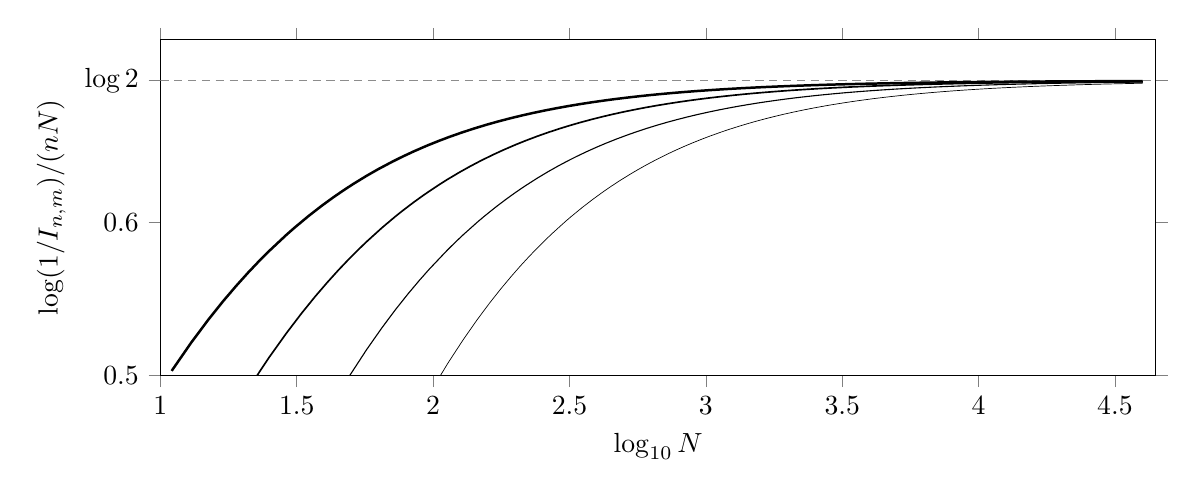
\begin{tikzpicture}
\begin{axis}[width=5.6in,height=2.3in,xmin=1,xmax=4.65,ymin=0.5,ymax=0.72,
xlabel={$\log_{10}N$},ylabel={$\log(1/I_{n,m})/(nN)$},ytick={0.5,0.6,0.6931},yticklabels={$0.5$,$0.6$,$\log2$},
axis background/.style={fill=white},tick align=outside]
\addplot[black!45,densely dashed,domain=1:4.65,samples=2]{0.6931};
\addplot[black,line width=0.9pt] coordinates {(1.0414,0.50283)(1.1139,0.52158)(1.1761,0.53645)(1.2304,0.54860)(1.2788,0.55874)(1.3222,0.56736)(1.3617,0.57480)(1.3979,0.58129)(1.4624,0.59210)(1.4914,0.59666)(1.5441,0.60451)(1.5911,0.61104)(1.6335,0.61657)(1.6721,0.62132)(1.7076,0.62545)(1.7559,0.63073)(1.7993,0.63517)(1.8513,0.64010)(1.8865,0.64322)(1.9294,0.64681)(1.9777,0.65056)(2.0212,0.65369)(2.0607,0.65636)(2.1038,0.65907)(2.1492,0.66173)(2.1959,0.66427)(2.2380,0.66639)(2.2810,0.66840)(2.3243,0.67029)(2.3674,0.67203)(2.4099,0.67362)(2.4518,0.67508)(2.4955,0.67650)(2.5378,0.67776)(2.5809,0.67896)(2.6243,0.68007)(2.6675,0.68110)(2.7101,0.68203)(2.7536,0.68292)(2.7973,0.68374)(2.8395,0.68447)(2.8825,0.68516)(2.9258,0.68580)(2.9689,0.68639)(3.0116,0.68692)(3.0550,0.68743)(3.0980,0.68789)(3.1408,0.68831)(3.1838,0.68870)(3.2271,0.68907)(3.2697,0.68939)(3.3128,0.68970)(3.3558,0.68998)(3.3988,0.69024)(3.4417,0.69048)(3.4847,0.69070)(3.5278,0.69090)(3.5709,0.69109)(3.6137,0.69126)(3.6568,0.69141)(3.6998,0.69156)(3.7426,0.69169)(3.7857,0.69181)(3.8286,0.69192)(3.8716,0.69202)(3.9146,0.69212)(3.9576,0.69220)(4.0005,0.69228)(4.0435,0.69235)(4.0865,0.69242)(4.1294,0.69248)(4.1724,0.69254)(4.2153,0.69259)(4.2583,0.69264)(4.3013,0.69268)(4.3443,0.69272)(4.3872,0.69276)(4.4302,0.69279)(4.4732,0.69282)(4.5161,0.69285)(4.5591,0.69287)(4.6020,0.69290)};
\addplot[black,line width=0.6pt] coordinates {(1.1139,0.42689)(1.2304,0.46420)(1.3222,0.49105)(1.3979,0.51147)(1.4624,0.52762)(1.5185,0.54078)(1.5682,0.55173)(1.6128,0.56101)(1.6532,0.56900)(1.6902,0.57595)(1.7243,0.58207)(1.7559,0.58751)(1.8129,0.59675)(1.8633,0.60434)(1.8865,0.60765)(1.9294,0.61350)(1.9685,0.61851)(2.0212,0.62484)(2.0531,0.62844)(2.0969,0.63310)(2.1367,0.63707)(2.1732,0.64050)(2.2175,0.64441)(2.2577,0.64772)(2.3032,0.65123)(2.3365,0.65363)(2.3820,0.65672)(2.4232,0.65932)(2.4609,0.66154)(2.5011,0.66376)(2.5378,0.66566)(2.5809,0.66774)(2.6201,0.66951)(2.6599,0.67118)(2.6998,0.67275)(2.7396,0.67420)(2.7789,0.67555)(2.8176,0.67678)(2.8579,0.67797)(2.8993,0.67911)(2.9390,0.68013)(2.9773,0.68105)(3.0175,0.68194)(3.0573,0.68276)(3.0966,0.68351)(3.1364,0.68423)(3.1764,0.68489)(3.2162,0.68550)(3.2555,0.68606)(3.2951,0.68659)(3.3347,0.68707)(3.3746,0.68753)(3.4138,0.68795)(3.4535,0.68834)(3.4932,0.68870)(3.5331,0.68904)(3.5725,0.68934)(3.6120,0.68963)(3.6518,0.68990)(3.6913,0.69014)(3.7309,0.69037)(3.7706,0.69058)(3.8103,0.69078)(3.8498,0.69096)(3.8895,0.69113)(3.9291,0.69128)(3.9685,0.69142)(4.0081,0.69156)(4.0479,0.69168)(4.0874,0.69179)(4.1270,0.69190)(4.1665,0.69199)(4.2061,0.69208)(4.2457,0.69216)(4.2853,0.69224)(4.3249,0.69231)(4.3645,0.69238)(4.4041,0.69244)(4.4437,0.69249)(4.4833,0.69254)(4.5229,0.69259)(4.5624,0.69263)(4.6020,0.69267)};
\addplot[black,line width=0.4pt] coordinates {(1.2304,0.33447)(1.3979,0.40172)(1.5185,0.44503)(1.6128,0.47566)(1.6902,0.49866)(1.7559,0.51668)(1.8129,0.53123)(1.8633,0.54328)(1.9085,0.55344)(1.9494,0.56214)(1.9868,0.56970)(2.0531,0.58219)(2.0828,0.58742)(2.1106,0.59213)(2.1614,0.60025)(2.1847,0.60378)(2.2279,0.61002)(2.2672,0.61535)(2.3032,0.61998)(2.3365,0.62402)(2.3820,0.62924)(2.4232,0.63365)(2.4609,0.63743)(2.4955,0.64072)(2.5276,0.64360)(2.5670,0.64694)(2.6031,0.64983)(2.6365,0.65234)(2.6749,0.65506)(2.7168,0.65784)(2.7490,0.65984)(2.7846,0.66194)(2.8228,0.66405)(2.8579,0.66587)(2.8949,0.66766)(2.9330,0.66940)(2.9680,0.67090)(3.0073,0.67247)(3.0434,0.67382)(3.0795,0.67509)(3.1156,0.67628)(3.1514,0.67738)(3.1889,0.67847)(3.2256,0.67945)(3.2613,0.68036)(3.2978,0.68122)(3.3330,0.68200)(3.3701,0.68277)(3.4057,0.68346)(3.4423,0.68412)(3.4784,0.68473)(3.5149,0.68531)(3.5516,0.68585)(3.5880,0.68635)(3.6242,0.68681)(3.6598,0.68724)(3.6963,0.68765)(3.7325,0.68803)(3.7689,0.68838)(3.8052,0.68871)(3.8412,0.68902)(3.8777,0.68930)(3.9139,0.68957)(3.9500,0.68982)(3.9863,0.69005)(4.0227,0.69027)(4.0588,0.69047)(4.0951,0.69066)(4.1313,0.69083)(4.1675,0.69099)(4.2037,0.69115)(4.2400,0.69129)(4.2760,0.69142)(4.3124,0.69154)(4.3486,0.69165)(4.3847,0.69176)(4.4210,0.69186)(4.4571,0.69195)(4.4934,0.69203)(4.5295,0.69211)(4.5658,0.69219)(4.6020,0.69226)};
\addplot[black,line width=0.25pt] coordinates {(1.5185,0.30063)(1.6902,0.37926)(1.8129,0.42842)(1.9085,0.46257)(1.9868,0.48790)(2.0531,0.50757)(2.1106,0.52335)(2.1614,0.53634)(2.2068,0.54725)(2.2480,0.55656)(2.2856,0.56461)(2.3201,0.57166)(2.3522,0.57788)(2.3820,0.58342)(2.4099,0.58839)(2.4362,0.59288)(2.4843,0.60068)(2.5065,0.60409)(2.5478,0.61013)(2.5855,0.61532)(2.6201,0.61984)(2.6522,0.62381)(2.6821,0.62733)(2.7235,0.63192)(2.7490,0.63461)(2.7846,0.63818)(2.8176,0.64130)(2.8579,0.64491)(2.8859,0.64727)(2.9206,0.65005)(2.9528,0.65248)(2.9899,0.65513)(3.0175,0.65699)(3.0558,0.65943)(3.0853,0.66121)(3.1183,0.66309)(3.1538,0.66500)(3.1867,0.66667)(3.2214,0.66833)(3.2536,0.66977)(3.2871,0.67120)(3.3183,0.67244)(3.3535,0.67377)(3.3861,0.67493)(3.4191,0.67603)(3.4522,0.67708)(3.4830,0.67799)(3.5181,0.67897)(3.5506,0.67983)(3.5826,0.68062)(3.6158,0.68140)(3.6483,0.68211)(3.6813,0.68279)(3.7147,0.68344)(3.7470,0.68403)(3.7805,0.68461)(3.8138,0.68514)(3.8466,0.68564)(3.8790,0.68610)(3.9117,0.68654)(3.9453,0.68696)(3.9780,0.68734)(4.0110,0.68771)(4.0436,0.68805)(4.0763,0.68837)(4.1094,0.68867)(4.1422,0.68895)(4.1750,0.68922)(4.2080,0.68947)(4.2408,0.68970)(4.2734,0.68992)(4.3062,0.69012)(4.3393,0.69032)(4.3720,0.69050)(4.4050,0.69067)(4.4376,0.69083)(4.4706,0.69097)(4.5034,0.69111)(4.5362,0.69124)(4.5691,0.69137)(4.6019,0.69148)};
\end{axis}
\end{tikzpicture}
\caption{The lower bound of Proposition~\ref{selb} for $\psi(N)/N$, with $m=1,2,4,8$ from the thickest curve to the thinnest. Raising the power of the auxiliary polynomial does not raise the constant above $\log2$.}\label{figsel}
\end{figure}

The reason is visible in the proof. A power of the polynomial raises the degree in the same proportion as the order of vanishing, so the ratio that decides the constant does not move. Nair, Chudnovsky and Pritsker studied this method for polynomials in several variables, and Pritsker \cite{pritsker} describes the constants it can reach in terms of weighted capacity. Stepanov's proof escapes this proportion through Step 3 of Theorem~\ref{stepanov}. The Frobenius map makes $f$ agree with the much smaller function $\delta(f)$ at every rational point, so the order of vanishing $M$ is paid for by the dimension of $L(\ell M+n)$ and not by the degree of $f$. The test therefore sharpens what a lift has to do. A lift must raise the order of vanishing at a cost that is smaller than the cost of raising the degree. In the archive the mechanism has two sides, which Section~\ref{sec:gainmech} states. The lattice $N_u$ is a sublattice of the base lattice of bounded colength, scaled up by an explicit power of each inert prime, and the degree formula for a sublattice turns this into \eqref{A2}. The composite of the lifts is divisible by that power on the sublattice, and the archive uses this divisibility for the integrality of the period pairing on the scaled lattice, which is part of the statement R2 of Section~\ref{sec:remain}.

\subsection{The setting of one lift in the archive}\label{sec:setting}

This subsection states the setting of the seven hypotheses of Proposition~\ref{acct} in ordinary terms, as the archive defines it. The next four paragraphs transcribe definitions of the archive.

The lattices live over the ring of integers of a totally complex Galois number field $K$ that contains the cyclotomic field of Section~\ref{sec:acct}. There is one hermitian lattice $R$, and for each $u\in W$ a hermitian lattice $N_u$ together with a $K$-linear pairing $B_u$ between $N_u\otimes K$ and $R\otimes K$. The archive states that $B_u$ takes values in the integers of $K$ on $N_u\times R$ exactly when $\varphi\mapsto B_u(\varphi,\cdot)$ maps $N_u$ into the dual lattice $R^\vee$. Hypothesis \eqref{A3} is the slope inequality for that map, with $\mu^C$ the slope of $R^\vee$ and $h_u$ the height of $B_u$. A further statement identifies $B_u$ with a Bessel period.

The numbers $a_t$ are weights. The archive ties them to the highest weight of the forms on a unitary group of rank $k$, whose first and last coordinates are $a_t+\tfrac{k-1}2$ and $-b_t-\tfrac{k-1}2$, and it places the integers $a_t$ in a short window above a common size $a$ with $a/b$ within one of $x$. The variable $x$ of the sum over primes is therefore the ratio of a weight to a node.

The three quantities $\Phi$, $\Gamma$ and $E_u$ are sums over the finite places $w$ of $K$. With $\sigma(w,y)=2\,\ell_w\,e_w\,y$, where $\ell_w$ is the logarithmic size of $w$ and $e_w$ its ramification index,
\begin{gather*}
\Phi=\sum_{j=1}^m\sum_w\sigma\big(w,F_j(w)\big),\qquad
E_u=\sum_{j=1}^m\sum_w\sigma\big(w,E_{u,j}(w)\big),\\
\Gamma=\sum_w\sigma\Big(w,\sum_{j=1}^m\mathrm{gain}_j(w)-\tau(w)\Big),
\end{gather*}
and $\mathrm{gain}_j(w)$ vanishes unless the residue characteristic of $w$ lies in one of two classes of primes that the archive calls signal and inert. The right side of \eqref{A4} appears in the archive verbatim, with $\log\Omega=\gamma+\log(\pi/v)-L'(1,\chi)/L(1,\chi)$, which has the shape of the logarithm of a CM period in the formula of Chowla and Selberg that Alp\"oge's note lists.

With these readings the four main hypotheses say the following. By \eqref{A1}, the sum over primes is at most the total gain in divisibility that the $m$ lifts produce at the finite places. By \eqref{A2}, the slope of $N_u$ exceeds the slope of a base lattice by that gain, up to the local terms $\Phi$ and $E_u$. By \eqref{A3}, the period pairing is integral. By \eqref{A4}, the archimedean size of the pairing is at most $m$ times a quantity close to $\sum_t\log\Gamma(a_t)$, measured against the CM period. The product formula then forces the finite gain, and with it the sum over primes, below the archimedean size. The target for one lift is the case $m=1$ of \eqref{A2} and \eqref{A4} for these objects. Section~\ref{sec:gainmech} states the objects behind \eqref{A2} and what the archive proves about them, and Section~\ref{sec:archside} does the same for \eqref{A3} and \eqref{A4}.

\subsection{A second test, Taylor coefficients at a CM point}\label{sec:taylor}

Alp\"oge's note dates its second step as a divisibility statement for an invariant derivation on a CM curve at a prime that is inert in the CM field. The simplest example of such a statement can be computed exactly, and it shows the size of the effect.

Let $E_2,E_4,E_6$ be the Eisenstein series of level one and $D=\frac1{2\pi i}\frac d{d\tau}$. Ramanujan's identities say that $D'=12D$ acts on the ring $\mathbb Z[E_2,E_4,E_6]$ by
\[
D'E_2=E_2^2-E_4,\qquad D'E_4=4(E_2E_4-E_6),\qquad D'E_6=6(E_2E_6-E_4^2).
\]
At the CM point $\tau=i$ the nonholomorphic derivative $\partial$ of a modular form is computed by the same derivation with $E_2$ replaced by a function that vanishes at $i$, and $E_6(i)=0$, as Zagier explains in \cite[\S5]{zagier}. Hence, for every integer $r\ge0$, the derivative of order $2r$ at $i$ is
\[
\partial^{2r}E_4(i)=12^{-2r}\,C_r\,E_4(i)^{r+1},
\]
where the integer $C_r$ is the coefficient of $E_4^{\,r+1}$ in $D'^{\,2r}E_4$ after setting $E_2=E_6=0$. The point $i$ has complex multiplication by $\mathbb Z[i]$, in which a prime $p$ is inert when $p\equiv3\pmod4$ and split when $p\equiv1\pmod4$.

We computed $C_r$ exactly for $0\le r\le110$, starting $1,20,360,25920,984960$. Figure~\ref{figtay} shows the result for the inert primes $7$ and $11$. For the inert primes $7,11,19,23,31$ the average of $v_p(C_r)/2r$ over $60\le r\le110$ is $0.040$, $0.015$, $0.0053$, $0.0030$, $0.0023$, against the values $0.042$, $0.017$, $0.0056$, $0.0038$, $0.0021$ of $2/(p^2-1)$. The split primes $13,17,29,37,41$ do not divide any $C_r$ in this range.

\begin{figure}[htbp]
\centering
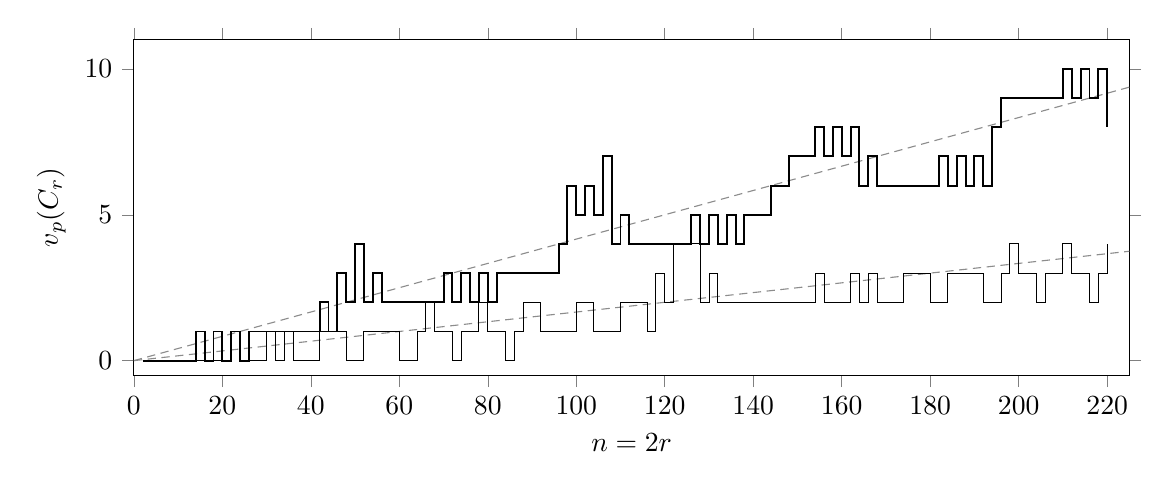
\begin{tikzpicture}
\begin{axis}[width=5.6in,height=2.3in,xmin=0,xmax=225,ymin=-0.5,ymax=11,
xlabel={$n=2r$},ylabel={$v_p(C_r)$},axis background/.style={fill=white},tick align=outside]
\addplot[black!45,densely dashed,domain=0:225,samples=2]{2*x/48};
\addplot[black!45,densely dashed,domain=0:225,samples=2]{2*x/120};
\addplot[black,const plot,line width=0.7pt] coordinates {(2,0)(4,0)(6,0)(8,0)(10,0)(12,0)(14,1)(16,0)(18,1)(20,0)(22,1)(24,0)(26,1)(28,1)(30,1)(32,1)(34,1)(36,1)(38,1)(40,1)(42,2)(44,1)(46,3)(48,2)(50,4)(52,2)(54,3)(56,2)(58,2)(60,2)(62,2)(64,2)(66,2)(68,2)(70,3)(72,2)(74,3)(76,2)(78,3)(80,2)(82,3)(84,3)(86,3)(88,3)(90,3)(92,3)(94,3)(96,4)(98,6)(100,5)(102,6)(104,5)(106,7)(108,4)(110,5)(112,4)(114,4)(116,4)(118,4)(120,4)(122,4)(124,4)(126,5)(128,4)(130,5)(132,4)(134,5)(136,4)(138,5)(140,5)(142,5)(144,6)(146,6)(148,7)(150,7)(152,7)(154,8)(156,7)(158,8)(160,7)(162,8)(164,6)(166,7)(168,6)(170,6)(172,6)(174,6)(176,6)(178,6)(180,6)(182,7)(184,6)(186,7)(188,6)(190,7)(192,6)(194,8)(196,9)(198,9)(200,9)(202,9)(204,9)(206,9)(208,9)(210,10)(212,9)(214,10)(216,9)(218,10)(220,8)};
\addplot[black,const plot,line width=0.35pt] coordinates {(2,0)(4,0)(6,0)(8,0)(10,0)(12,0)(14,0)(16,0)(18,0)(20,0)(22,1)(24,0)(26,0)(28,0)(30,1)(32,0)(34,1)(36,0)(38,0)(40,0)(42,1)(44,1)(46,1)(48,0)(50,0)(52,1)(54,1)(56,1)(58,1)(60,0)(62,0)(64,1)(66,2)(68,1)(70,1)(72,0)(74,1)(76,1)(78,2)(80,1)(82,1)(84,0)(86,1)(88,2)(90,2)(92,1)(94,1)(96,1)(98,1)(100,2)(102,2)(104,1)(106,1)(108,1)(110,2)(112,2)(114,2)(116,1)(118,3)(120,2)(122,4)(124,4)(126,4)(128,2)(130,3)(132,2)(134,2)(136,2)(138,2)(140,2)(142,2)(144,2)(146,2)(148,2)(150,2)(152,2)(154,3)(156,2)(158,2)(160,2)(162,3)(164,2)(166,3)(168,2)(170,2)(172,2)(174,3)(176,3)(178,3)(180,2)(182,2)(184,3)(186,3)(188,3)(190,3)(192,2)(194,2)(196,3)(198,4)(200,3)(202,3)(204,2)(206,3)(208,3)(210,4)(212,3)(214,3)(216,2)(218,3)(220,4)};
\end{axis}
\end{tikzpicture}
\caption{The $p$-adic valuation of the integer $C_r$, which gives the Taylor coefficient of order $n=2r$ of $E_4$ at the CM point $i$, for the inert primes $p=7$ (thick) and $p=11$ (thin). The dashed lines are $2n/(p^2-1)$.}\label{figtay}
\end{figure}

The divisibility at inert primes is real and grows linearly with the order of the derivative. Its rate is $2n/(p^2-1)$, and the sum of $\frac{2n}{p^2-1}\log p$ over all primes is a constant times $n$. At $r=110$ the inert primes contribute $28.6$ to $\log C_r=933.2$, while $n\log n-n=966.6$. A sum over primes of the size that Section~\ref{sec:acct} needs requires a gain of order $a/p$ at each prime $p$, which is the size of the $p$-adic valuation of a factorial. One derivative at one CM point of a form of level one therefore does not produce the gain of hypothesis \eqref{A1}. In the archive the gain comes from the large weights $a_t$, through the estimate \eqref{valest} of Section~\ref{sec:gainmech}. Congruences for Taylor coefficients at CM points modulo inert primes are known from the work of Larson and Smith \cite{larsonsmith} and, for the Jacobi theta constant, from a conjecture of Romik \cite{romik}. We did not find the rate $2n/(p^2-1)$ stated in this form, and we present it as an observation from the computation.

\subsection{The gain of a lift in the archive}\label{sec:gainmech}

This subsection explains how the archive obtains hypothesis \eqref{A2}, and how it proves and uses the divisibility that gives the gain its meaning. The statements are theorems of the archive and are not proved in this paper. Their proofs have been reconstructed from the Lean text, and the last paragraph of the subsection records their status.

The number $\mathrm{gain}_j(w)$ of Section~\ref{sec:setting} is defined in the archive by the closed formula \eqref{gainformula} below, and two statements about lattices give it its meaning. Fix an index $u$ and a place $w$ over a prime $p$ of the inert class. At $w$ the archive has a local form $M_w$ of the base lattice, of rank $d$, and a part $M_w^{\mathrm{ram}}$ of it in a subspace that the archive specifies. Let $\mathcal K_m$ be the composite of the $m$ lifts, and let $\mathrm{Int}_m$ be the integral structure of the forms at the top of the chain. The archive constructs a sublattice $N\!P_w$ of $M_w^{\mathrm{ram}}$ such that
\begin{equation}\label{twosides}
\operatorname{length}\big(M_w^{\mathrm{ram}}/N\!P_w\big)\le\operatorname{ord}_w(p)\,d\,\big(\tau(w)+\mathrm{io}(w)\big),\qquad
\mathcal K_m\big(N\!P_w\big)\subset p^{\,s_u(w)}\,\mathrm{Int}_m ,
\end{equation}
where $s_u(w)=\sum_{j=1}^m\big(\mathrm{gain}_j(w)+F_j(w)-E_{u,j}(w)\big)$, the number $\tau(w)$ is the term of $\Gamma$ in Section~\ref{sec:setting}, $\mathrm{io}(w)$ is a second local term, and $\operatorname{ord}_w(p)$ is the valuation of $p$ in the local ring. The first statement bounds a colength and the second is a divisibility. The archive's statement \texttt{admG1} is this pair for a lattice with a chain of maps on it, and the two halves reach the final theorem of the archive on different routes. Hypothesis \eqref{A2} uses the colength bound. The proof of the statement \texttt{LinkG} below verifies \texttt{admG1} for a chain whose maps are all zero, for which the divisibility holds trivially, so that proof does not use the valuation estimate of this subsection. The divisibility for the lifts themselves is a separate theorem of the archive. It has the column map of the lifts in the place of $\mathcal K_m$ and an exponent of the form of $s_u(w)$ with one further term, and it leads to R2. The end of this subsection follows that route.

The colength bound is the loss side. It rests on a statement that the archive calls \texttt{LPprime}, which concerns a Hecke operator $y_o$ on the base lattice, attached to a Frobenius orbit $o$ at $p$. The statement says that $y_o$ is nondegenerate up to a bounded power of $p$ on a share $1-\kappa$ of the rank, and the archive calls the orbits at which it applies the statement served. The lattice $N\!P_w$ is built from the images of the powers $y_o^m$ at the served orbits, and the nondegeneracy bounds its colength, which is how the terms $\tau(w)$ and $\mathrm{io}(w)$ arise. So \texttt{LPprime} is a statement of nondegeneracy that controls the loss. It is not a divisibility statement, and the archive does not derive the gain from it.

The divisibility is the gain side, and it comes from an estimate for the kernel of one lift. Let $p\ge5$ be a prime and consider one Frobenius orbit at $p$, of even length $2\nu$, with positions $s\in\mathbb Z/2\nu$. Let $\mathcal T$ be the set of the positions that are tops, which are the positions that have one of the weights $a_t$. At this orbit the kernel of the lift from level $j$ to level $j+1$ is a power series $\Theta$ in the entries of matrices $X_s$ of size $N_j\times N_{j+1}$, one for each position, with $N_j=k+j(t+1)$. The estimate has the hypothesis that $\Theta=\exp(-\Upsilon)\,U$, where $U$ is integral in the parameter of a formal group of height two and $\Upsilon$ is, up to a series whose exponential is integral, a sum of values of a pairing that is additive in each variable and semilinear for the Frobenius of $\mathbb Q_{p^2}$. The archive proves this hypothesis for the theta kernel in a theorem that we call the kernel law (\texttt{first\_kernel\_law\_global\_small}), and the next three paragraphs state its content and the structure of its proof.

Let $\mathcal C$ be an elliptic curve with complex multiplication by the integers of $\mathbb Q(\sqrt{-d})$ and with good reduction at $p$, let $\mathsf t$ be a parameter of its formal group, and let $z(\mathsf t)$ be the complex coordinate of $\mathcal C$ as a power series in $\mathsf t$, which is a unit multiple of the logarithm of the formal group. Let $\vartheta(z)$ be the product of the Weierstrass sigma function of the period lattice of $\mathcal C$ and of $e^{-s_2z^2/2}$, where $s_2$ is the constant formed from the quasi-periods for which $|\vartheta(z)|^2e^{-\pi|z|^2/A}$ is periodic for the lattice, with $A$ the area of a period parallelogram. The archive puts
\[
\phi(\mathsf t)=-\log\frac{\vartheta\big(z(\mathsf t)\big)}{z'(0)\,\mathsf t},\qquad
\beta(\mathsf t,\mathsf t')=\phi\big(\mathsf t+_{\mathcal C}\mathsf t'\big)-\phi(\mathsf t)-\phi(\mathsf t'),
\]
where $+_{\mathcal C}$ is the addition of the formal group, so $\beta$ is the coboundary of $\phi$ for the group law. Write $f\simeq g$ when the exponential of $f-g$ has integral coefficients. The archive states that $\beta$ is additive in each variable up to $\simeq$, that $\phi([a]\mathsf t)\simeq a\bar a\,\phi(\mathsf t)$ for multiplication by an integer $a$ of $\mathbb Q(\sqrt{-d})$ of norm prime to $p$, and that $\beta([a]\mathsf t,\mathsf t')\simeq\beta(\mathsf t,[\bar a]\mathsf t')$. At a prime $p$ that is inert in $\mathbb Q(\sqrt{-d})$ the formal group of $\mathcal C$ has height two, the integers of $\mathbb Q(\sqrt{-d})$ are dense in the integers of $\mathbb Q_{p^2}$, and complex conjugation becomes the Frobenius of $\mathbb Q_{p^2}$. Inertness therefore turns the last relation into the semilinearity of $\beta$ for that Frobenius. The kernel law is stated for $p\ge5$, and in its proof this enters as the condition that $p$ does not divide $6$.

The kernel $\Theta$ is the expansion at the origin of a theta function on a power of $\mathcal C$, attached to a pair of hermitian lattices. In coordinates $\mathsf t_1,\dots,\mathsf t_r$ along a basis of the lattice of the pair that is orthonormal at $p$, the archive states that
\[
\exp\Big(\sum_{i=1}^r\phi(\mathsf t_i)\Big)\,\Theta\quad\text{is integral.}
\]
The entries of the matrices $X_s$ are coordinates of a different kind. The variables at the even positions and the variables at the odd positions span two isotropic subspaces for the hermitian form that are in duality, which is a hyperbolic frame, and the odd positions are the embeddings composed with complex conjugation. The three properties of $\phi$ and $\beta$ above make $\phi$ behave as a hermitian quadratic form with associated pairing $\beta$, up to $\simeq$. The archive proves from them that the change from the orthonormal coordinates to the hyperbolic frame turns $\sum_i\phi(\mathsf t_i)$ into a sum of values of $\beta$ at the pairs of dual variables (\texttt{hypShape}), and the integrality in orthonormal coordinates becomes
\[
\Theta=\exp(-\Upsilon)\,U,\qquad U\ \text{integral},\qquad\Upsilon\simeq\sum_e\beta(x_e,y_e),
\]
with $x_e$ at the even positions and $y_e$ at the odd ones. A classification statement of the archive, \texttt{BetaIsG}, then puts the pairing in the normal form that the valuation estimate uses. The kernel law is stated in a parameter of the formal group with logarithm $\sum_{j\ge0}x^{p^{2j}}/p^j$, to which the formal group of $\mathcal C$ is isomorphic at an inert prime. In such a parameter every pairing that is additive in each variable and semilinear in the sense above is, up to $\simeq$, a constant times the series $\sum_{0\le i\le j}x^{p^{2i}}y^{p^{2j+1}}/p^{\,i+j+1}$ minus the Frobenius image of that constant times the same series with $x$ and $y$ exchanged.

The archive obtains the integrality in orthonormal coordinates from theta functions of rank one. It reduces a general pair of lattices to a pair that is standard at $p$, that case to rank two, and rank two to rank one. For rank one the fourth tensor power of the theta function is, in suitable unitary coordinates, a product of translates of $\vartheta$ by points of order prime to $p$. A statement in one variable says that such a translate is $e^{-\phi}$ times an integral series (\texttt{lubin\_tate\_transfer\_integral}). Its proof writes the $N$th power of a translate by a point of order $N$ as a product of unit series, by the addition formula for the sigma function in the parameter of the formal group, and it takes an $N$th root, which is integral because $p$ does not divide $N$. A second statement passes from the integrality of a fourth tensor power to the integrality of the series itself (\texttt{general\_integrality}), and it rests on the invariance of $\sum_i\phi(\mathsf t_i)$ under unitary changes of the variables up to $\simeq$. Both statements rest on lemmas of formal calculus on a Weierstrass curve with good reduction. The kernel law has the hypothesis that an elliptic curve with complex multiplication by the integers of a field $\mathbb Q(\sqrt{-d})$ has good reduction over an unramified extension at every prime $l\ge5$ that does not divide $d$. The archive derives that hypothesis from global Artin reciprocity and the main theorem of complex multiplication, which it quotes as published theorems, and from a statement of Chebotarev type that it proves.

The weight of level $j+1$ at a position $s$, shifted to have nonnegative coordinates, is a Young diagram. Let $\alpha_s$ be the number of its columns of height one when $s\in\mathcal T$, and $\alpha_s=0$ otherwise, let $\mathrm{cap}_s$ be the number of its other columns, and let $\mathrm{box}_s$ be the number of boxes in those. At a top, $\alpha_s$ is the difference of the first two coordinates of the base weight, which the archive ties to the weight $a_t$. For $s\in\mathcal T$ let $\mathcal E(s)$ be the set of the residues of $s'-s$ modulo $2\nu$ in $\{0,\dots,2\nu-1\}$, for the tops $s'$ whose parity differs from that of $s$. Let $\operatorname{lg}_p(0)=0$ and $\operatorname{lg}_p(y)=\lfloor\log_py\rfloor+1$ for an integer $y\ge1$, and put
\[
\Delta=\sum_s\Big(N_{j+1}\operatorname{lg}_p(\alpha_s)+N_jN_{j+1}\operatorname{lg}_p(\mathrm{box}_s)\Big)+\sum_{s\in\mathcal T}\operatorname{lg}_p(\alpha_s)^2 .
\]
Let $Y_s$ be a square matrix of auxiliary variables of size $N_j$, and let $P$ be a product, over the positions $s$ and over the columns of the diagram at $s$, of minors of $Y_sX_s$, where a column of height $h$ gives a minor on the first $h$ rows and on $h$ columns of our choice. The value at the origin of $P(\partial_X)\Theta$ is a polynomial in the auxiliary variables. The estimate says that every coefficient $c$ of this polynomial, for every choice of the columns, has a $p$-adic valuation
\begin{equation}\label{valest}
v_p(c)\ \ge\ \sum_{s\in\mathcal T}\ \sum_{\substack{i\ \mathrm{odd}\\ i\notin\mathcal E(s)}}\max\Big(\frac{\alpha_s}{p^i}-\mathrm{cap}_{s+i},\,0\Big)-\Delta .
\end{equation}

The archive proves \eqref{valest} in two parts. The first part says that after the substitution $X\mapsto\varpi X$ with $\varpi^{p^2-1}=p$ the kernel is a sum $\sum_{i\ge0}p^{-i}\,\mathfrak h^i\,g_i$ with integral series $g_i$, for an explicit series $\mathfrak h$ with integral coefficients. Modulo $p$, each monomial of $\mathfrak h$ is the product of a power $p^{2l+1}$ of a variable at a position $s-2l$ and a power $p^{2l'}$ of a variable at the position $s+1-2l'$. This part rests on the kernel law and on two internal statements, \texttt{BetaIsG} and a congruence that the archive calls \texttt{TwoSumsCondition}. Their proofs reduce to a classical lemma on the integrality of a formal group law. The second part is the bound \eqref{valest} for every series of that form, and its proof is elementary. The chain of statements of the archive that leads from the second part to the divisibility of the lifts and to R2 is
\begin{gather*}
\texttt{Top.entry\_a\_one}\ \to\ \texttt{G7.kernel\_a\_one\_generic}\ \to\ \texttt{ea\_A1U}\ \to\ \texttt{first\_theorem\_place\_bound}\\
\to\ \texttt{VolumeRatio}_2\ \to\ \texttt{stmt\_proved}\ \to\ \texttt{unit\_bound\_of\_sum\_over\_primes}\\
\to\ \texttt{sum\_over\_primes\_service}\ \to\ \texttt{admissible\_level\_two}\ \to\ \texttt{linkDIVt\_closedK}\ \to\ \texttt{LinkDIV}.
\end{gather*}
The archive also has a chain from \texttt{stmt\_proved} through \texttt{admG1} to a second proof of \texttt{LinkG}, named \texttt{linkG\_of}, and its final theorem does not use that proof. A statement of similar content, \texttt{SeriesGaussValuationFirst}, is a definition of a proposition in the archive, and the chain above does not use it.

The form of \eqref{valest} has the following explanation, which summarizes its proof. For generic values of the auxiliary variables the minors of size one at a top $s$ form a power of order $\alpha_s$ of one linear form. The pairing with this power produces a factorial, whose valuation is about $\alpha_s/(p-1)$, and the substitution $X\mapsto\varpi X$ subtracts $\alpha_s/(p^2-1)$. The difference is the credit $\alpha_s\,p/(p^2-1)=\sum_{i\ \mathrm{odd}}\alpha_s/p^i$ of the top $s$. Each factor $p^{-1}$ in the kernel comes with a factor $\mathfrak h$. After a change of variables that separates the direction $z_s$ of the linear form, the monomials of $\mathfrak h$ that can meet $P$ are $z_s^{\,p^i}$ times one variable at the position $s+i$ with $i$ odd, which is the position that $i$ Frobenius steps reach from $s$. One such factor uses $p^i$ of the $\alpha_s$ units of degree at $s$, so at most $\alpha_s/p^i$ of them occur. It also uses one first derivative of a minor at $s+i$. A determinant is linear in each column, so the minors at $s+i$ absorb at most $\mathrm{cap}_{s+i}$ such derivatives. Credit minus debit is the sum in \eqref{valest}. The set $\mathcal E(s)$ accounts for the monomials of $\mathfrak h$ that join two tops, and $\Delta$ accounts for the digits in Legendre's formula for the factorials. The bound follows from the ultrametric inequality, term by term, and the proof does not use a cancellation. The auxiliary variables are taken generic so that the largest coefficient of the polynomial is the norm of one of its values.

The shifts $i$ are odd because the two variables in such a monomial of $\mathfrak h$ sit at positions that differ by an odd number. This is the semilinearity of the pairing for the Frobenius of $\mathbb Q_{p^2}$, which forces the exponents $p^a$ and $p^b$ of a monomial of the pairing to have $a-b$ odd. The normal form of \texttt{BetaIsG} stated above has this property, and the semilinearity is its hypothesis.

At the served orbits the archive improves the bound, and this improvement is a separate argument. Two further estimates, \texttt{EntryCappedBound} and \texttt{EntryB}, have the same proof as \eqref{valest} up to its last count. They say that after a Hecke operator at the orbit on the target of the lift the tops at even positions keep their whole credit $\alpha_s\,p/(p^2-1)$, without the capacity term and without the exclusions. A commutation relation between the Hecke operators and the lifts then moves the operator to the source at an explicit price.

The number $\mathrm{gain}_j(p)$ is the resulting exponent, written in the global parameters. For an orbit $o$ at $p$ let $\mathrm{base}_j(p,o)$ be the right side of \eqref{valest} with quantities defined from the weights $a_t$ and the nodes of Section~\ref{sec:setting} in place of $\alpha_s$, $\mathrm{cap}_s$ and $\Delta$, let $\mathrm{impr}_j(p,o)$ be the improved bound in the same parameters, and let $\mathrm{price}_j(p,o)$ be the price. Write $\mathrm{base}_j^+=\max(\mathrm{base}_j,0)$. With the arguments $(p,o)$ omitted on the right, the archive defines
\begin{equation}\label{gainformula}
\mathrm{gain}_j(p)=\sum_{o\ \mathrm{served}}\max\big(\mathrm{impr}_j-\mathrm{price}_j,\ \mathrm{base}_j^+\big)+\sum_{o\ \text{not served}}\mathrm{base}_j^+
\end{equation}
for the primes at which the gain does not vanish, which lie in the two classes of Section~\ref{sec:setting} and below a bound. So $\mathrm{gain}_j(w)$ is a defined number, and the archive does not estimate it. It is an explicit lower bound for the exponent that the valuation estimates give for $\mathcal K_m$ on $N\!P_w$, once a comparison of numbers and three further statements are granted. The first passes from a bound for all the coefficients $c$ above to an inclusion of lattices, and the second writes a lift as a sum of kernel maps over classes of lattices. These two are hypotheses of the valuation chain, and the archive states them for the lifts inside the theorem \texttt{SysTw} below. The third, \texttt{LowTermBound}, combines the $m$ lifts and the served orbits by an induction, with a statement \texttt{FormB} on the Hecke sums. Under \texttt{LowTermBound} the archive proves that a Hecke operator on the target of one lift is a triangular combination of the lifts of Hecke operators on the source (\texttt{hk\_point}), from a count of lattices over a discrete valuation ring with Gaussian binomial coefficients (\texttt{countLoc}), and it inverts this relation along the chain by symmetric functions (\texttt{G7.theorem\_c\_i}).

The colength bound of \eqref{twosides} and the definition of the gain meet in the slope of $N_u$. Let $M_u$ be the base lattice with its part $M_u^{\mathrm{ram}}$, and let $\Lambda_u$ be the sublattice of $M_u^{\mathrm{ram}}$ that is given by $N\!P_w$ at the places $w$ outside the prime $T_u$. With $\mathfrak p_w$ the prime ideal of $w$, the archive defines
\begin{equation}\label{Nscale}
N_u=\Big(\prod_w\mathfrak p_w^{-\lfloor e_w\,s_u(w)\rfloor}\Big)\Lambda_u ,
\end{equation}
with the gain set to zero at a set of primes that it drops, so the gain enters the slope of $N_u$ by definition. The degree formula for a sublattice of full rank, which is classical, gives
\begin{equation}\label{degform}
\mu(N_u)=\mu\big(M_u^{\mathrm{ram}}\big)+\sum_w\sigma\Big(w,\ \frac{\lfloor e_w\,s_u(w)\rfloor}{e_w}-\frac{\operatorname{len}_u(w)}{\operatorname{rk}N_u}\Big),
\end{equation}
where $\operatorname{len}_u(w)$ is the colength of $\Lambda_u$ at $w$. The colength bound of \eqref{twosides}, inserted in \eqref{degform}, gives the archive's statement \texttt{SlopesN}. This is \eqref{A2} with the terms $\Gamma$, $\Phi$ and $E_u$ of Section~\ref{sec:setting}, and with an error $e_2$ that contains the terms $\mathrm{io}(w)$, the integer parts and the places above the prime $T_u$. The archive's statement \texttt{LinkG} contains the colength bound for $\Lambda_u$ together with inequalities between the defined numbers, and \eqref{A2} follows from \texttt{LinkG}, from R1 of Section~\ref{sec:remain} and from \eqref{degform}. The proof of \texttt{LinkG} that the final theorem of the archive uses (\texttt{linkG\_concrete5}) is the one with the zero maps described after \eqref{twosides}. So \texttt{LinkG} and \eqref{A2} do not depend on the valuation estimate, and the gain occurs in them as the defined number \eqref{gainformula}.

The divisibility of the lifts is used for R2, and the archive reaches R2 from \eqref{valest} in four steps. First, at a place $w$ over an inert prime $p\ge5$ outside a finite set, the archive has a model of the chain of lifts at $w$ for which the hypotheses of the valuation chain hold. This is its theorem \texttt{SysTw}. Among these hypotheses are the form $\exp(-\Upsilon)\,U$ of the kernel, which is the kernel law above, the passage from bounds for coefficients to inclusions of lattices, and the expression of a lift as a sum over classes. A further statement, \texttt{CmpV}, says that divisibility in the model implies divisibility of the column map of the lifts, and the archive obtains it from comparison maps that intertwine each lift with its model. Second, the valuation chain and these two statements give the divisibility of the column map of the lifts on $N\!P_w$ by $p$ to an exponent of the form of $s_u(w)$ (\texttt{sum\_over\_primes\_service}). At the places without a gain the same theorem uses separate bounds for the columns. Third, a pairing of the columns with a lattice of forms turns this into a lower bound for the valuation at $w$ of the period pairing, under integrality hypotheses on the periods (\texttt{admissible\_level\_two}). Fourth, this bound is an input of the proof of \texttt{LinkDIV} (\texttt{linkDIVt\_closedK}), which contains R2. The top level of that proof confirms the role of the scaling in \eqref{Nscale}. The target lattice $R$ is defined place by place, and at $w$ it is spanned by the forms with which the columns are paired, so a pairing that is divisible by a power of $p$ at $w$ still maps into the dual lattice after the source lattice is enlarged by that power. The archive derives R1 from \texttt{LinkDIV} in the theorem that produces \texttt{LinkDIV}.

The gain side is therefore reconstructed as mathematics. The kernel law reduces to theta functions of rank one and to the translates of a theta function in one variable, which follow from the addition formula for the sigma function, and the valuation estimate is elementary once the kernel has the form $\exp(-\Upsilon)\,U$. The route from the divisibility of the lifts to \texttt{LinkDIV} passes through the model of the chain at an inert place, the bounds for the columns, and the pairing with the lattice of forms. On the loss side the archive proves the nondegeneracy statement \texttt{LPprime} from standard monomial theory for integral forms of representations of a general linear group, with the Pieri and branching rules and the extremal projector of Asherova, Smirnov and Tolstoy, and the explicit constants of these classical inputs have not yet been compared with printed sources. None of the internal packages of Section~\ref{sec:status} lies on the gain side or on the loss side. The published inputs of this subsection are global Artin reciprocity, the good reduction of elliptic curves with complex multiplication, and the theory of formal groups, and Section~\ref{sec:archside} continues with the archimedean half of the route.

\subsection{The archimedean side, the covolume bound and the Galois inputs}\label{sec:archside}

This subsection explains how the archive obtains hypotheses \eqref{A3} and \eqref{A4} and the two bounds of R4. The statements are theorems of the archive whose proofs have been reconstructed from the Lean text, and they are not proved in this paper. A paragraph headed \emph{Reconstruction status} marks each place where an internal package of Section~\ref{sec:status} remains.

Hypothesis \eqref{A4} is the last of the conditions of R2, and its right side is the sum of two bounds. The first is a bound for the height $h_u$ of the map $B_u$. This map is the composite of the $m$ lifts followed by a pairing with forms on a second unitary group, and the archive bounds its norm at each archimedean place by the product of the norms of these $m+1$ maps (\texttt{height\_chain\_atR}). It then defines $h_u$ by a closed formula in which each lift contributes, at each embedding, the number
\[
\sum_i\big(\operatorname{ph}(\nu_i)-\nu_i\log\Omega\big),
\]
where the $\nu_i$ are the degrees of the kernel of that lift in its variables. A comparison of numbers in the archive bounds the sum of these contributions by the term $\sum_t\big(m\operatorname{ph}(a_t)-m\,a_t\log\Omega\big)$ of \eqref{A4} up to the errors there. So the factor $m$ in front of $\operatorname{ph}(a_t)$ counts the lifts, which confirms the reading of Section~\ref{sec:acct}.

The constant $\log\Omega$ is a period. The kernel law of Section~\ref{sec:gainmech} needs the kernel in the parameter of a model of $\mathcal C$ with good reduction, and the archimedean norm is computed in the complex coordinate. The two coordinates differ by the period of the model, and the archive proves that a mean of the logarithm of this period, taken over a number field of definition of the model, equals
\[
\log\Omega=\gamma+\log\frac{\pi}{v}-\operatorname{Re}\frac{L'(1,\chi_d)}{L(1,\chi_d)}
\]
(\texttt{MeanPeriod}), which is the formula of Chowla and Selberg~\cite{chowlaselberg}. The same logarithmic derivative occurs in Proposition~\ref{inert}, and the two occurrences cancel in the proof of Proposition~\ref{acct}.

The second bound is an upper bound for the slope of the dual lattice $R^\vee$. The archive obtains it from lattices of forms on the second group, one for each level of the chain, whose covolumes it bounds by arithmetic intersection theory on a unitary Shimura variety (\texttt{L3}, \texttt{CovolumeBoundOfX}). The identification of $B_u$ with a period on the second group is a further condition of \texttt{LinkDIV} (\texttt{BesselId}). The covolume bound has two parts. The first is an effective arithmetic Hilbert--Samuel inequality on one good deep cover (\texttt{HSAt}), proved by a Chow-form determinant argument in the style of Nesterenko and Philippon. The determinant of the coordinate polynomials of a well-chosen basis of the top lattice is divisible by a fixed power of the Chow form of the image, and additivity, a lower bound of Gelfond type for Mahler heights, a Hadamard inequality and a count of monomials give a lower bound for the arithmetic degree with every constant explicit. The geometric inputs are Kawamata--Viehweg vanishing, a Bertini theorem and the existence and integrality of Chow forms, and the Bergman bound is a sub-mean-value inequality times the mass of a fundamental set. Every constant depends on the rank, the degree and the size of the weight, so the inequality is uniform over all components of all good deep covers. The second part is a lower bound for mean volume slopes, which the next paragraphs describe.

The deepest input of the covolume bound is a uniform lower bound for mean volume slopes over deep covers (\texttt{DeepStR}). For a component $Z$ of a deep cover of the Shimura variety and a weight $u$ with a gap, let $\mathrm{sl}_Z(u)$ be the exponential growth rate, normalized by the degree, of the number of cusp forms on $Z$ of weight a multiple of $u$ that are integral at the primes below a cutoff $B$ and have bounded sup norm. With $B$ of polynomial size in $u$ and its gap, the statement is
\[
\frac1{\lvert\mathrm{Comp}\rvert}\sum_{Z\in\mathrm{Comp}}\mathrm{sl}_Z(u)\ \ge\ -C\Big(\big(\log B+\log\mathrm{rd}_E+\big\lvert\operatorname{Re}\tfrac{L'}{L}(1,\chi_d)\big\rvert\big)\lVert u\rVert_1+q\,\mathrm{spread}(u)\Big),
\]
where $\mathrm{Comp}$ is the set of components, $\mathrm{rd}_E$ is the root discriminant of $E$, $q$ is the smaller index of the signature, $\mathrm{spread}(u)$ is the sum over the CM types of the range of the entries of $u$, and $C$ does not depend on the field, the level or the weight. The proof works on a tower of integral models indexed by the cutoff $B$, on which the arithmetic self-intersection $P_B(u)$ of the Hodge line bundle of weight $u$ is a polynomial in $u$. First, the slope of the tower is a limit of slopes of nef hermitian line bundles. Second, the successive minima of Zhang force $P_B$ to vanish on the Weyl walls up to $O(\log B/B)$. Third, antisymmetry under the simple reflections reduces $P_B$, up to the same error, to the form
\[
\operatorname{vol}\cdot\big(h_{\mathrm{Fl}}-\alpha\,\mathrm{Sh}-\beta\,\mathrm{Tot}\big),
\]
where $h_{\mathrm{Fl}}$ is the height of the flag variety and $\mathrm{Sh}$ and $\mathrm{Tot}$ are the functionals of the first Chern classes of a partial sum and of the total sum of the Hodge bundles. Fourth, at each good prime $p$ above the cutoff an exact identity gives the change of the arithmetic intersection numbers under the change of integral structure at $p$, as a term $\log p/(p-1)$, the discrepancy between the de Rham and Hodge--Tate lattices, plus a series in the powers of Frobenius. Letting $B\to\infty$ in this identity turns the asymptotic form into an exact identity at every finite cutoff, and the constants of the first three steps, which depend on the tower and hence on the level, disappear. Fifth, a test polynomial and a lower bound for the heights of points bound the two remaining coefficients. Sixth, these bounds give a lower bound for $P_B(u)$, hence for the mean slope of the tower, and a lattice-point transfer moves it to the components at the cost of an explicit sum over the primes below $B$. So the uniformity does not come from controlling every integral model uniformly at the level primes. It comes from the cutoff limit together with the exact identity at good primes. The constants that survive come from heights of points, through the formula of Chowla and Selberg for $\mathbb Q(\sqrt{-d})$ and a slope bound of Bost's type for Lie algebras, from cusp weights on fundamental sets, from the first Chern class at the bad primes and from sums of Mertens type over at most $B$ primes. The CM period is that of $\mathbb Q(\sqrt{-d})$, and no formula of Colmez is used. The archive restricts to levels with at most fifteen prime factors, and this restriction serves to bound the number of bad primes by the cutoff, with a large margin. The slope bound of Bost's type for Lie algebras, which enters the heights of points, has not yet been matched with a printed source.

The exact identity at good primes is local, and it explains both the term $\log p/(p-1)$ and the Frobenius series. Fix a good prime $p$, put $w=\zeta_p-1$, so that $w^{p-1}=u\,p$ for a unit $u$, and for a label $\tau$ of a Frobenius orbit let $\mathrm{Lie}_\tau$ and $W_\tau$ be the de Rham and Hodge--Tate lattices of the abelian scheme, with the dual lattices $\omega_\tau\supseteq\omega^{\mathrm{HT}}_\tau$. Fargues's integral Hodge--Tate sequence gives the sandwich
\[
\mathrm{Lie}_\tau\subseteq W_\tau\subseteq w^{-1}\mathrm{Lie}_\tau,\qquad \omega^{\mathrm{HT}}_\tau\subseteq\omega_\tau\subseteq w^{-1}\omega^{\mathrm{HT}}_\tau .
\]
Write $\mathrm{ck}_k(E,E')$ for the change of the $k$-th power-sum Chern class between two lattices with the same generic fibre, intersected with a fixed cycle $Q$ on the special fibre. Put $h_\tau=(-1)^k\sum_i\mathrm{ck}_k(X_{\tau,i},T)$, where the $X_{\tau,i}$ are the coordinate lines of the $\mathbb F$-vector space scheme $G[p]$ in the character attached to $\tau$ and $T$ is the trivial line, and put $\lambda_\tau=k\,\mathrm{rootNum}_{\mathrm{Lie}_\tau}(p_{k-1},Q;p)$, the intersection with the divisor of $p$. Then
\[
\mathrm{ck}_k(\mathrm{Lie}_\tau,W_\tau)+\mathrm{ck}_k(\omega_\tau,\omega^{\mathrm{HT}}_\tau)=h_\tau-\frac{\lambda_\tau}{p-1},\qquad p^kh_\tau=h_{\mathrm{Fr}\tau}+\lambda_{\mathrm{Fr}\tau}.
\]
The first relation follows from the exact sequence $0\to w^{-1}\mathrm{Lie}_\tau/W_\tau\to H/T_n\to\omega_\tau/\omega^{\mathrm{HT}}_\tau\to0$ given by the kernel and image of the Hodge--Tate map, together with $(p-1)\,\mathrm{rootNum}(w)=\mathrm{rootNum}(p)$, so the term $\lambda_\tau/(p-1)$ is the divisor of $\zeta_p-1$. The second follows from a filtration $K_0\supset\dots\supset K_n=pK_0$ whose graded pieces are $X_{\mathrm{Fr}\tau,i}/X_{\tau,i}^{\otimes p}$, together with $\mathrm{ck}_k(X^{\otimes p})=p^k\,\mathrm{ck}_k(X)$, so the factor $p^k$ is the effect of Frobenius on the $k$-th power-sum Chern class of a line. On a finite orbit the recursion has the unique solution
\[
h_\tau=\sum_{n\ge0}p^{-k(n+1)}\lambda_{\mathrm{Fr}^{n+1}\tau},
\]
which is the series in the powers of Frobenius of the fourth step, and a descent from an extension of the discrete valuation ring gives the comparison of Chern classes that the identity uses. The classes $\mathrm{ck}$ and $\mathrm{rootNum}$ are defined on a chosen flag model, and reading them as intrinsic quantities uses statements of flag independence.

\paragraph{Reconstruction status.} The lower bound for mean volume slopes, its descent through the cutoff limit, the two lattice relations, the solution of the recursion, the point-height constant and the sums of Mertens type have been reconstructed. Two internal packages remain. The first is local, and it is the proof that the lattice family of the $p$-torsion group scheme satisfies the test-point facts $\ker H_\tau=(\zeta_p-1)^{-1}\mathrm{Lie}_\tau$, $\operatorname{im}H_\tau=\omega_\tau$ and the Frobenius step on coordinates (\texttt{FamEx.TestPt.testFacts}), together with the construction of the family, the Chern calculus on models over a discrete valuation ring and flag independence. Its mechanism agrees with Raynaud's description of $\mathbb F$-vector space schemes and Fargues's integral Hodge--Tate sequence, but the archive proves these facts internally, and that proof has not yet been reconstructed to the literature boundary. The second is global. It consists of the existence of the cutoff tower and of its qualitative axioms (\texttt{exists\_good\_tower}), the lattice-point transfer below its top, and the covolume statements beside the mean-slope bound, among them theta spanning at minimal level, a nonvanishing level determinant and the estimate $\log\mathrm{supConst}\le250f^2r^2L$ of the Bergman constant behind $\log\beta\le4000z^3$. Its mechanisms are standard Arakelov geometry of the tower, and the constants of the tower axioms disappear in the cutoff limit.

Hypothesis \eqref{A3} is the archive's statement \texttt{FrameF}, which Section~\ref{sec:discussion} displays. The archive derives it from a theorem on a family of integral maps $B_u$ from lattices $N_u$ into one lattice. Let $Q=\sum_u\gamma_uB_uB_u^{*}$ with positive weights $\gamma_u$, formed at one archimedean place in orthonormal frames. The theorem assumes that each $\gamma_uB_u^{*}B_u$ is close to the identity in the Hilbert--Schmidt norm and that $\operatorname{tr}(Q^2)$ is close to $(\operatorname{tr}Q)^2$ divided by the dimension, so that $Q$ is close to a scalar, and it concludes the inequality of \texttt{FrameF}. Its proof is an argument of slope theory. It combines the filtration of Harder and Narasimhan for hermitian lattices \cite{stuhler,grayson} with the slope inequality of Bost \cite{bost} and a count of the ranks of the images of the pieces of that filtration at the archimedean place, and it does not use the arithmetic of the lifts. The archive derives the two assumptions from the statement \texttt{LinkIRR} of Section~\ref{sec:discussion} and from Hilbert--Schmidt bounds (\texttt{LinkS}), which it states for the Gram operators of the Poincar\'e series attached to two indices $u\ne u'$. The passage from these operators to the maps $B_u$ runs in one direction. The nonvanishing of the Poincar\'e series (\texttt{PuNZ}) follows from the diagonal dominance of their Gram matrix on the side of \texttt{LinkS}. It is the input of the identity of theta integrals behind the records (\texttt{MIstar2}), and that identity gives the identification \texttt{BesselId} of $B_u$ with a Bessel period, which transports the bounds of \texttt{LinkS} to the maps $B_u$ of \texttt{LinkDIV} and \texttt{FrameF}. The order is therefore \texttt{LinkS}, \texttt{PuNZ}, \texttt{MIstar2}, \texttt{BesselId}, then \texttt{LinkDIV} and \texttt{FrameF}, and there is no circular dependency. The archimedean input of \texttt{LinkS} is the decay of Bessel transforms on the unitary group, and it rests on identities for the radial parts $F_l$ of Capelli-type invariant operators acting on the Bessel function at the points of a torus with coordinates $c_l$. Expanding the quantum minors that define these operators along their border row and column, using the two-sided $N$-equivariance of the Bessel function, which removes every border term except the one at the neighboring site, and using $c\,\partial_c\lvert c\rvert^{\lambda}=\tfrac\lambda2\lvert c\rvert^{\lambda}$, one obtains the three-term recursion
\[
F_l=(Y+c_l\partial_{c_l})\,F_{l+1}-c_{l+1}c_l^{-1}\,F_{l+2},
\]
with $Y$ the spectral variable, so the radial parts are entries of a product of $2\times2$ transfer matrices. The decay of the Bessel transform itself, which the archive calls Theorem~P, is proved by computing the transform in stages over a Heisenberg extension, with a Leibniz rule for one letter, a telescoping collapse by the quantum determinant and a cutoff removed by dominated convergence. In the model algebra of the cutoff argument the collapse is the RLL relation of a Lax matrix with entries in a Weyl algebra and the $R$-matrix of Yang, $R(Y-Y')=(Y-Y')\cdot1-P$, together with the quantum determinant relation $T(Y+1)^{\mathsf T}JT(Y)=J$. Both have been reconstructed and checked symbolically, and the one-letter collapse of the model reduces to them and to an eigenvalue hypothesis. A few finite rearrangements in the commutant algebra and the analytic imports of the steps belong to the small leaves of Section~\ref{sec:status}.

The counting side of \texttt{LinkS} and \texttt{LinkIRR} counts discrete series in spaces of cusp forms. The multiplicity of a discrete series representation whose Harish-Chandra parameter has a large gap is expressed by a pre-trace formula whose test function is a matrix coefficient of that representation. Square integrability and the weighted integrability of matrix coefficients of discrete series make the geometric side absolutely convergent, and the geometric side is split into four regions of the group, called near, far, deep and rare, which are bounded separately. The bounds are lattice counts, through mean values of primitive sublattices over a genus in the spirit of Siegel and Schmidt and a factorization of the counting kernel over finitely many places. The constants of these counts enter the later thresholds as a single lower bound that is uniform over the family, so no smallness of them is used.

\paragraph{Reconstruction status.} The pre-trace formula, its division into regions and the dependence of the later thresholds on the counting constants have been reconstructed. The remaining internal package is the lattice-counting layer. It consists of the proofs of five mean-count lemmas with their shared first step (\texttt{count\_terms\_gramClass\_over\_sublattice}), the local factorization of the counting kernel and the leaves of the counting engine. The mechanism is the mean value theorem of Siegel and Schmidt's counts of sublattices. One compatibility check is open in this package, between the level idempotents of the dimension clause of \texttt{LinkS} and the hypothesis of a near-unipotent count (\texttt{NearUnip}).

The two bounds of R4 control the local terms of the lifts at the places where their local type is twisted. The bound \texttt{LinkN} concerns a congruence module, the quotient of the projection of the lattice of integral forms onto a Hecke summand by the lattice of integral forms that lie in that summand. The archive bounds the congruence ideal of the summand by the lengths of Selmer groups through a universal cocycle, and those lengths are the quantity that \texttt{VWin} bounds. The cocycle is lifted to integral crystalline lattices with exponents that come from Wach modules, and three estimates give these exponents. The torsion bound for crystalline extensions with trivial quotient follows from the theorems of Tate, Sen, Fontaine, Wach, Berger and Bloch--Kato, with an explicit constant that grows like the logarithm of the size of the Hodge weights, as the point inequality of the route needs. The Wach module is realized through Berger's description of the Wach lattice by filtration conditions at the points $\zeta_{l^{s+1}}-1$, with a Frobenius bootstrap on annihilator ideals. The generic lifting exponent comes from a descent along a generator $\gamma$ of the cyclotomic Galois group. If $\pi^H\mathcal N\subset\mathcal N'$ for two Wach modules, removing one power of $\pi$ costs a factor $u^k-1$ with $u=\chi(\gamma)$, and the valuations of these factors for $k\le H$ add up to
\[
\Big\lfloor\frac H{l-1}\Big\rfloor+v_l\Big(\Big\lfloor\frac H{l-1}\Big\rfloor!\Big)\le\frac{Hl}{(l-1)^2},
\]
which is the main term of the exponent.

Two further lifting theorems, which the archive calls Theorems~B and~C, treat Wach modules whose Hodge jumps alternate between large and small at consecutive embeddings, which the archive calls thick and thin letters. Theorem~B transports classes along arcs of embeddings. Its core is a relay map, built from the solution of a $\gamma$-equation in a frame of the Wach module, a truncation of Frobenius images at the cost $l^\sigma$ with $\sigma\approx2h\,l/(l-1)^3$, and saturation, and its case bounds are at most $40\,\mathrm{Sg}$ plus a band term, where $\mathrm{Sg}=h/l^2+(w+S+\eta)/l+\log_l(2h)+1$ and $\sigma\le3\,\mathrm{Sg}$ for $l\ge11$. Theorem~C treats arcs on which every letter is thick. There the power of the Frobenius element gained at one embedding is divided by the power of the Wach element at the next, the sizes of the two intermediate letters cancel exactly, and the size $b$ of the first letter survives as $b/l$ through the Newton polygon, so that an up step followed by a down step behaves like a thin letter. The final bound is $e\le32H/l^2+4S+10\eta/(l-1)+25\lambda$, whose leading coefficient at $l=11$ is $31.108$.

\paragraph{Reconstruction status.} The relay of Theorem~B with its $\gamma$-equation, truncation, saturation, transport and uniqueness, the eight interior lemmas of Theorem~C with their supplier, and the constants $40\,\mathrm{Sg}$, $\sigma\le3\,\mathrm{Sg}$ for $l\ge11$ and $32$ at $l=11$ have been reconstructed. The two theorems rest on one shared package of Wach-module calculus, which remains under audit. It contains Berger's membership criterion along an arc with its level maps (\texttt{LevC.secCrit\_all} for Theorem~B and \texttt{expCrit\_D'} for Theorem~C), the truncation of Frobenius images with its level expansion, the annihilating polynomials in $\gamma$, three fields of the generic lifting package, and the case bodies and interior tools above them. The mechanism is completely known, the expected published inputs are the theorems of Wach, Berger, Herr, Benois and Fontaine, and several proof bodies remain unread.

For the generic part of \texttt{VWin} the archive bounds the length of a Selmer group by the valuations of $\operatorname{tr}\rho(\sigma)-t$ over the automorphic points $\rho$ of a deformation ring of a reducible residual representation, where $t$ is the trace of the reducible representation at $\sigma$. It then bounds the sum of those valuations over all primes by the height of one nonzero integer, and a count of automorphic forms bounds that height. This step rests on the automorphy of every point of the deformation ring, a statement that the archive proves internally. First-order deformations are bounded by the theorem of Greenberg and Wiles with explicit local conditions, after a limit passage by counting and the Artin--Rees lemma, and the residually reducible case uses generalized matrix algebras in the sense of Bella\"iche and Chenevier. These are the hypotheses of the rank-three statement \texttt{P3core}, and every point of a chain to which it is applied is nice. The first-order bound \texttt{x1} follows from Mazur's presentation of the deformation ring by an obstruction theory and from the Euler characteristic inequality $h^2+h^0+2d\le h^1$, which gives $b+2+2d\le a+2g$. At the primes where generic position fails the archive passes to rank four. There a Hida family in characteristic $l$ has constant pseudo-character, and automorphy propagates between the minimal primes of the deformation ring along irreducible curves, by a bound for the dimension of the reducible loci and by a presentation of the ring whose number of relations is controlled by the global Euler characteristic. The dimension bound \texttt{red} comes from a bound for the tangent space, a degeneration to a split point along a cocharacter and a count of odd roots, which give $\dim\mathrm{Tan}(S,c_0)\le d+20C$. The crossing in rank four passes through irreducible nice curves, so it involves neither the rank-three statement nor thick primes, but it uses the exponent of the first-order bound through the start of its chain of points. The auxiliary place at which the frame condition holds comes from the Chebotarev density theorem (\texttt{V0ok}). The standard leaves of the rank-four argument and the patching lemmas below these mechanisms belong to the small leaves of Section~\ref{sec:status}. R4 enters the route in one place, as a hypothesis of \texttt{LinkDIV} at the places where the local type of the forms is twisted, and R5 uses R4 through the bound $V\le\sqrt b$.

\subsection{The records and the seesaw identities}\label{sec:records}

The lattices, heights and local terms of R1 and R2 are the fields of a record, and R1 to R4 are relations between these fields. The content of the geometric core is therefore the existence of a family of records. The archive derives it from published theorems through four intermediate statements, which are an identity of theta integrals (\texttt{MIstar2}), the existence of matched local data, the covolume bound of Section~\ref{sec:archside} and the bound R4. The proof that assembles the records from these statements is a list of eight steps.

The identity of theta integrals is a seesaw. The groups of the tower of lifts are definite, so the automorphic forms on them are finite vectors of polynomial functions on frames, and the period integrals reduce to finite sums over classes. Howe duality for $(GL_a,GL_b)$ on polynomial functions, multiplicity-one branching from $U(n+1)$ to $U(n)$, Schur's lemma and the irreducibility of Weyl modules give the laws for kernels, periods and readings at each step. The finite-place part of the identity is the value of a double step. For a step $j$ with Fourier--Jacobi subgroup $J$ and Bessel subgroup $B$, the double integral over $J\backslash U(V_{j+1})(\mathbb A_f)$ and $B\backslash U(V_{j+2})(\mathbb A_f)$ of the product of two Weil-translated vacua with a column reading is a Bessel period of the step $j+2$ times
\[
c_V(j)=\kappa(j,\sigma)\,\mathrm{sc}_j\,\mathrm{sc}_{j+1}\,c_Q(j)\,c_G(j)\,c_T(j),\qquad c_Q(j)=\prod_{q\in Q}\big(\mathrm{idx}_q(j+1)\,\mathrm{idx}_q(j+2)\big)^{-1}.
\]
The proof is a chain of six exact identities. Base points are moved at the cost $\mathrm{sc}_j\,\mathrm{sc}_{j+1}$, Heisenberg combinations at disjoint sets of places commute, the integral collapses to the twist places $Q$ with the factor $\kappa$, which is a ratio of volumes of one open compact subgroup, the integral at the twist places gives $c_Q$, and the kernel data give $c_G\,c_T$. At the level places the middle variable enters both Weil actions, which multiply the two vacua by $a^{-1}$ and $a$, and the two scalars cancel in the bilinear product. The value at the twist places reduces, by induction on the number of twist places and Fubini over places, to a local double-step identity at one split place, where $U(V)\cong GL_n$ and the Weil representation is the linear model $\omega(g,h)\Phi(x)=\mu(\det g,\det h)\,\Phi(h^{-1}xg)$. That identity rests on the root exchange of Ginzburg, Rallis and Soudry.

The coefficient of the whole identity for a tuple $\mathbf t$ of data is $c(\mathbf t)=c_{\mathrm{top}}(\mathbf t)\,s/c_{\mathrm{bot}}(\mathbf t)$, the product of the constants of the laws of the steps divided by the normalization constants of the theta lifts. The factors $\kappa$ and $c_G$ depend on the step and cancel in a ratio $c(\mathbf t)/c(\mathbf t_0)$, and the remaining factors differ by roots of unity, so the variation of the coefficient is bookkeeping with roots of unity.

\paragraph{Reconstruction status.} The seesaw value, its six identities, the constant $c_V$, the cancellation at the level places, the reduction of the twist-place laws to one split place, the root exchange and the unit property of $c(\mathbf t)$ have been reconstructed, and the laws for kernels, periods and readings are closed modulo the classical theorems named above. The remaining internal package is the finite-place harmonic analysis below these steps. It consists of the local double-step identity at a split place, whose first unread step is a trilinear form in the linear model (\texttt{GlobalTheory.TriStep.tri}), the laws at the level and unramified places in Schr\"odinger and mixed models, the producers of the data at the twist places, and the class data on which the laws are stated. The mechanism is known, and the expected named inputs are root exchange and Kudla's seesaw in the linear model.

The integral structure of the records comes from theta series. The integral forms on a cover of the tower descend to the base by Galois descent of coefficients and orthonormal integral bases of unramified extensions (\texttt{DescIntAt}). The theta kernel at a CM point is a classical short theta series over a coset of a lattice (\texttt{exists\_forms\_of\_transSum}), through Weil's dictionary between adelic and classical theta functions and a marking of the level structure. The first marking is built by the projective lifting property from the density of a global lattice in its completion. The resulting integrality statement gives, for a prime $l$, an exponent $c$ with $l^c\theta=\sum_k\beta_k\,\lambda\,c_c\,\mu\,\mathrm{rd}_U(f_k)$ and every $\beta_k$ integral, and $c$ is chosen before the level, so it is uniform in the level. In the archive the $\lambda$-integrality of a section is defined through its values at the good CM points, so integrality at those points is the definition used there and is not a separate theorem.

\paragraph{Reconstruction status.} The descent of integral forms, the identification of the kernel at CM points, the first marking and the level-uniform exponent have been reconstructed. Two marking theorems remain, the dual marking of a self-dual hermitian lattice (\texttt{Dict.DualMark.dual\_marking}) and the lift of marked points through level covers of the moduli space, together with seven producers of the integrality exponent and the Galois-side leaves behind them. They are small to medium, and their expected inputs are elementary lattice algebra and the existence of level structures on PEL moduli.

The remaining fields of the records are built in stages. The target lattice $R$ has a slope bound of the form $\mu_{\max}(R)\le x^{C_H}b-\operatorname{mean}_v\log\kappa_v$, through denominators of zeta values and toric periods (\texttt{FUN}), which feeds the covolume bound and \texttt{LinkDIV}. The stages of the record are built by assemblies over named statements, and eleven of them apply one published theorem each (\texttt{Open0}). The records are nonempty. The host field of Section~\ref{sec:host} is assembled (\texttt{hostOfFieldOf}) from the theory of quadratic and cyclotomic Dirichlet characters, the prime number theorem for primitive characters outside an exceptional zero, the construction of the field as the fixed field of the kernel of an Artin map, and Behrend's construction, and the nonvacuity of the records rests on a statement \texttt{HostEx} that the archive derives from nine published statements on the zeros of Dirichlet $L$-functions.

\paragraph{Reconstruction status.} The host size lemmas, the assembly of the host and the nonvacuity route have been reconstructed, and the nine analytic inputs of \texttt{HostEx} are on the external boundary. The remaining internal package is the construction of the records. Its bespoke part is the slope bound \texttt{FUN} with its sixteen leaves (\texttt{fun0Fit\_of\_leaves}), and the cores that build the stages of the record, the entries of \texttt{Open0} and \texttt{ON} and some leaves of the nonvacuity route are assemblies over named statements whose wiring is known. One compatibility check is open here, namely that the family constants can be chosen with $C_l\ge1.6\cdot10^{15}(C_g+4)$ and $\log\mathrm{rd}_E\le L/C_l$, which the gap condition of the lattice-counting package needs.

\section{The sum over primes of the route}\label{sec:ps}

This section identifies the sum over primes that the chain bounds. The first subsection proves the identity \eqref{eq:intro-inert}, and the second compares the gain at an inert prime that the identity requires with the valuations that Section~\ref{sec:taylor} computed for Taylor coefficients.

\subsection{The inert primes}\label{sec:primesum}

The archive defines the sum over primes $S$ of Proposition~\ref{acct} as follows. The definition runs over the Galois group of the cyclotomic field and a subset $\Phi$ of half of its elements. For a prime $p$ with Frobenius element $\sigma_p$ and for a weight $a$, the archive puts
\[
\mathrm{ask}_p=\sum_{i\ge1,\ \sigma_p^i\notin\Phi}\max\Big(\frac a{p^i}-w_{\rho(i,p)},\,0\Big),
\]
where the node $w_{\rho(i,p)}$ depends on the class $\sigma_p^i$, and it defines $S$ as the sum of $2\log p\cdot\mathrm{ask}_p$ over the primes with $\sigma_p\notin\Phi$, plus a similar term for one ramified prime $d$. It states an identity, \texttt{AskMainBalance}, that writes $S$ as the main term of \eqref{acctconc} plus a combination of the functions $G$ and $G_\chi$ of Section~\ref{sec:functions} over the characters $\chi$ of the Galois group. The gain of order $a/p$ that Section~\ref{sec:taylor} asked for is visible in $\mathrm{ask}_p$. We prove the identity in the case of one quadratic field, where $\Phi$ is the trivial subgroup.

\begin{proposition}[The sum over inert primes]\label{inert}
Let $d>3$ be a prime with $d\equiv3\pmod4$, let $\chi$ be the quadratic character modulo $d$, and call a prime $p$ inert when $\chi(p)=-1$. Let $G$ and $G_\chi$ be defined by \eqref{G} and \eqref{Gchi}. Then for all real numbers $a\ge w>0$,
\begin{multline*}
2\sum_{p\ \mathrm{inert}}\ \sum_{i\ \mathrm{odd}}\log p\,\max\Big(\frac a{p^i}-w,0\Big)+\log d\sum_{i\ge1}\max\Big(\frac a{d^i}-w,0\Big)\\
=a\Big(\log\frac aw-1-\gamma+\frac{L'(1,\chi)}{L(1,\chi)}\Big)+w\Big(G\Big(\frac aw\Big)-G_\chi\Big(\frac aw\Big)\Big).
\end{multline*}
\end{proposition}
\begin{proof}
For a prime power $n=p^i$ the number $1-\chi(n)$ equals $2$ when $p$ is inert and $i$ is odd, equals $1$ when $p=d$, and vanishes otherwise. Hence the left side is $\sum_{n\le a/w}\Lambda(n)(1-\chi(n))(a/n-w)$. With $y=a/w$ this is $w\sum_{n\le y}\Lambda(n)(y/n-1)-w\sum_{n\le y}\Lambda(n)\chi(n)(y/n-1)$, and the definitions \eqref{G} and \eqref{Gchi} give
\[
w\Big(G(y)+y\log y-(1+\gamma)y\Big)-w\Big(G_\chi(y)-\frac{L'(1,\chi)}{L(1,\chi)}\,y\Big),
\]
which is the right side.
\end{proof}

The primes that are inert in $\mathbb Q(\sqrt{-d})$ are the primes with $\chi(p)=-1$, and the main term on the right is the summand of \eqref{acctconc} with $\lambda_1=L'(1,\chi)/L(1,\chi)$. The route therefore bounds a sampled sum of $G-G_\chi$ from above. Theorem~\ref{engine} handles this sign under one extra hypothesis on real zeros.

\begin{corollary}[An upper bound for a difference]\label{corC}
Let $\chi_1,\dots,\chi_N$ be nontrivial Dirichlet characters, let $w_1,\dots,w_N$ be positive real numbers with $\sum_iw_i=1$, let $G$ and $G_\chi$ be defined by \eqref{G} and \eqref{Gchi}, and let $0\le\theta<1$. Suppose that $L(\beta,\chi_i)\ne0$ for every $i$ and every real $\beta$ with $\theta<\beta<1$, and that there are constants $\lambda>1$ and $C$ such that for arbitrarily large $Y$ the inequality $G(x)-\sum_iw_iG_{\chi_i}(x)\le Cx^\theta$ holds for every $x$ with $Y\le x\le Y^\lambda$. Then for every $s$ with $\operatorname{Re}s>\theta$ and $s\ne1$,
\[
m_\zeta(s)=\tfrac12\sum_{i=1}^Nw_i\big(m_{\chi_i}(s)+m_{\bar\chi_i}(s)\big).
\]
\end{corollary}
\begin{proof}
Apply Theorem~\ref{engine} to $H=G-\sum_iw_iG_{\chi_i}$, whose transform is $A=F-\tfrac12\sum_iw_i(F_{\chi_i}+F_{\bar\chi_i})$. By \eqref{res}, the poles of $A$ in $\operatorname{Re}s>\theta$ are simple, they lie in $\operatorname{Re}s<1$, and the residue at $\rho$ is $-d_\rho/(\rho(\rho-1))$ with $d_\rho=m_\zeta(\rho)-\tfrac12\sum_iw_i(m_{\chi_i}(\rho)+m_{\bar\chi_i}(\rho))$. A real pole in $(\theta,1)$ would be a real zero of $\zeta$ or of some $L(\cdot,\chi_i)$ or $L(\cdot,\bar\chi_i)$, and $L(\beta,\bar\chi_i)=\overline{L(\beta,\chi_i)}$ for real $\beta$, so $A$ does not have real poles in $(\theta,1)$ and the hypothesis of Theorem~\ref{engine} on real poles holds. The theorem gives $d_\rho=0$ for every $\rho$ with $\operatorname{Re}\rho>\theta$.
\end{proof}

Under the hypotheses of Corollary~\ref{corC} with one real character, a zero of $\zeta$ to the right of $\theta$ is a zero of $L(\cdot,\chi)$ of the same multiplicity. The archive has a statement of this form and separate hypotheses that exclude real zeros near $1$. In the final assembly of Section~\ref{sec:assembly} it bounds a positive combination $G_\Xi$, to which Corollary~\ref{corA} applies directly, so a common zero of the family is excluded by that corollary. Figure~\ref{figgd} shows the quantity for $d=7$, and we checked Proposition~\ref{inert} numerically at $a=54321$, $w=3.7$, where the two sides agree to $10^{-9}$.

\begin{figure}[htbp]
\centering
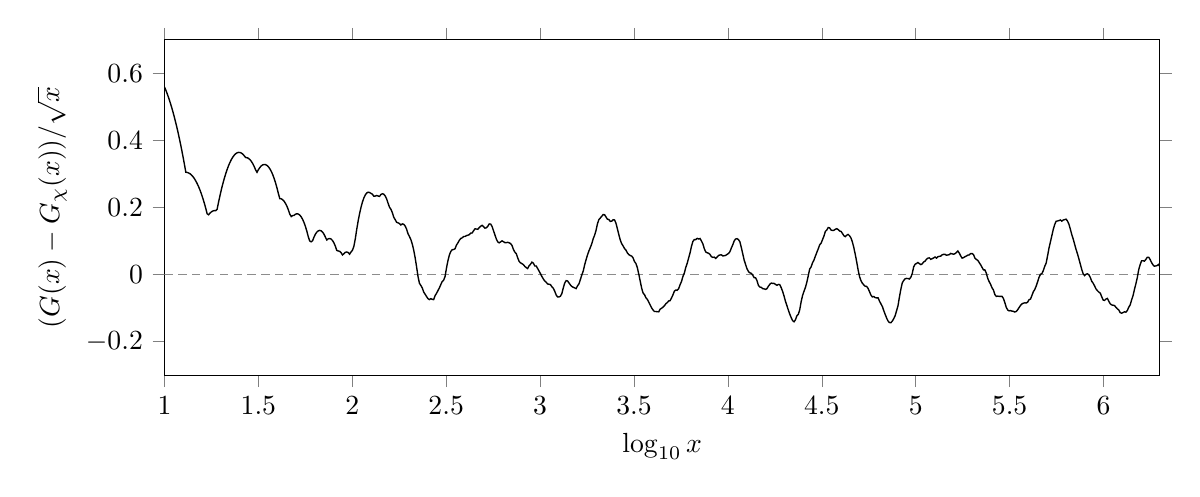
\begin{tikzpicture}
\begin{axis}[width=5.6in,height=2.3in,xmin=1,xmax=6.3,ymin=-0.3,ymax=0.7,
xlabel={$\log_{10}x$},ylabel={$(G(x)-G_\chi(x))/\sqrt x$},
axis background/.style={fill=white},tick align=outside]
\addplot[black!45,densely dashed,domain=1:6.3,samples=2]{0};
\addplot[black,line width=0.5pt] coordinates {(1.0000,0.55961)(1.0076,0.54947)(1.0152,0.53839)(1.0228,0.52638)(1.0303,0.51341)(1.0379,0.49949)(1.0455,0.48460)(1.0531,0.46873)(1.0607,0.45186)(1.0683,0.43400)(1.0758,0.41513)(1.0834,0.39524)(1.0910,0.37432)(1.0986,0.35235)(1.1062,0.32933)(1.1138,0.30525)(1.1213,0.30432)(1.1289,0.30292)(1.1365,0.30043)(1.1441,0.29683)(1.1517,0.29211)(1.1593,0.28627)(1.1668,0.27929)(1.1744,0.27117)(1.1820,0.26188)(1.1896,0.25143)(1.1972,0.23980)(1.2048,0.22697)(1.2123,0.21294)(1.2199,0.19770)(1.2275,0.18123)(1.2351,0.17822)(1.2427,0.18326)(1.2503,0.18704)(1.2578,0.18954)(1.2654,0.19077)(1.2730,0.19069)(1.2806,0.19505)(1.2882,0.21595)(1.2958,0.23552)(1.3033,0.25375)(1.3109,0.27063)(1.3185,0.28616)(1.3261,0.30031)(1.3337,0.31309)(1.3413,0.32447)(1.3489,0.33445)(1.3564,0.34301)(1.3640,0.35015)(1.3716,0.35585)(1.3792,0.36009)(1.3868,0.36287)(1.3944,0.36417)(1.4019,0.36398)(1.4095,0.36229)(1.4171,0.35908)(1.4247,0.35434)(1.4323,0.34894)(1.4399,0.34848)(1.4474,0.34644)(1.4550,0.34282)(1.4626,0.33759)(1.4702,0.33075)(1.4778,0.32228)(1.4854,0.31216)(1.4929,0.30487)(1.5005,0.31295)(1.5081,0.31933)(1.5157,0.32401)(1.5233,0.32697)(1.5309,0.32820)(1.5384,0.32767)(1.5460,0.32537)(1.5536,0.32130)(1.5612,0.31542)(1.5688,0.30772)(1.5764,0.29820)(1.5839,0.28682)(1.5915,0.27358)(1.5991,0.25845)(1.6067,0.24142)(1.6143,0.22647)(1.6219,0.22584)(1.6294,0.22325)(1.6370,0.21868)(1.6446,0.21213)(1.6522,0.20357)(1.6598,0.19297)(1.6674,0.18034)(1.6750,0.17302)(1.6825,0.17584)(1.6901,0.17657)(1.6977,0.17998)(1.7053,0.18129)(1.7129,0.18045)(1.7205,0.17744)(1.7280,0.17222)(1.7356,0.16479)(1.7432,0.15513)(1.7508,0.14320)(1.7584,0.12900)(1.7660,0.11250)(1.7735,0.10025)(1.7811,0.09763)(1.7887,0.10083)(1.7963,0.11184)(1.8039,0.12045)(1.8115,0.12664)(1.8190,0.13038)(1.8266,0.13166)(1.8342,0.13044)(1.8418,0.12672)(1.8494,0.12047)(1.8570,0.11166)(1.8645,0.10310)(1.8721,0.10665)(1.8797,0.10758)(1.8873,0.10586)(1.8949,0.10147)(1.9025,0.09438)(1.9100,0.08458)(1.9176,0.07204)(1.9252,0.07043)(1.9328,0.06927)(1.9404,0.06528)(1.9480,0.05846)(1.9556,0.06226)(1.9631,0.06630)(1.9707,0.06741)(1.9783,0.06558)(1.9859,0.06078)(1.9935,0.06732)(2.0011,0.07272)(2.0086,0.08421)(2.0162,0.10665)(2.0238,0.13482)(2.0314,0.15987)(2.0390,0.18178)(2.0466,0.20050)(2.0541,0.21603)(2.0617,0.22832)(2.0693,0.23736)(2.0769,0.24312)(2.0845,0.24556)(2.0921,0.24466)(2.0996,0.24220)(2.1072,0.23955)(2.1148,0.23347)(2.1224,0.23398)(2.1300,0.23582)(2.1376,0.23414)(2.1451,0.23301)(2.1527,0.23880)(2.1603,0.24098)(2.1679,0.23951)(2.1755,0.23436)(2.1831,0.22549)(2.1906,0.21288)(2.1982,0.20081)(2.2058,0.19470)(2.2134,0.18473)(2.2210,0.17088)(2.2286,0.16377)(2.2361,0.15588)(2.2437,0.15425)(2.2513,0.15202)(2.2589,0.14791)(2.2665,0.15102)(2.2741,0.15000)(2.2817,0.14480)(2.2892,0.13541)(2.2968,0.12176)(2.3044,0.11343)(2.3120,0.10429)(2.3196,0.09079)(2.3272,0.07289)(2.3347,0.05056)(2.3423,0.02374)(2.3499,-0.00493)(2.3575,-0.02575)(2.3651,-0.03238)(2.3727,-0.03976)(2.3802,-0.05183)(2.3878,-0.05847)(2.3954,-0.06523)(2.4030,-0.07149)(2.4106,-0.07472)(2.4182,-0.07179)(2.4257,-0.07379)(2.4333,-0.07461)(2.4409,-0.06283)(2.4485,-0.05612)(2.4561,-0.04789)(2.4637,-0.03973)(2.4712,-0.03009)(2.4788,-0.02080)(2.4864,-0.01679)(2.4940,-0.00596)(2.5016,0.01913)(2.5092,0.04110)(2.5167,0.05759)(2.5243,0.06856)(2.5319,0.07396)(2.5395,0.07476)(2.5471,0.07685)(2.5547,0.08793)(2.5622,0.09423)(2.5698,0.10206)(2.5774,0.10745)(2.5850,0.10944)(2.5926,0.11355)(2.6002,0.11354)(2.6078,0.11604)(2.6153,0.11735)(2.6229,0.11888)(2.6305,0.12352)(2.6381,0.12401)(2.6457,0.13048)(2.6533,0.13640)(2.6608,0.13586)(2.6684,0.13502)(2.6760,0.14014)(2.6836,0.14402)(2.6912,0.14683)(2.6988,0.14290)(2.7063,0.13826)(2.7139,0.13952)(2.7215,0.14401)(2.7291,0.15096)(2.7367,0.15086)(2.7443,0.14366)(2.7518,0.13092)(2.7594,0.11863)(2.7670,0.10614)(2.7746,0.09750)(2.7822,0.09467)(2.7898,0.09736)(2.7973,0.10043)(2.8049,0.09817)(2.8125,0.09514)(2.8201,0.09521)(2.8277,0.09615)(2.8353,0.09470)(2.8428,0.09250)(2.8504,0.08708)(2.8580,0.07501)(2.8656,0.06699)(2.8732,0.06264)(2.8808,0.04996)(2.8883,0.03945)(2.8959,0.03501)(2.9035,0.03252)(2.9111,0.02973)(2.9187,0.02433)(2.9263,0.02085)(2.9339,0.01796)(2.9414,0.02615)(2.9490,0.03088)(2.9566,0.03706)(2.9642,0.03406)(2.9718,0.02572)(2.9794,0.02571)(2.9869,0.01815)(2.9945,0.01051)(3.0021,0.00269)(3.0097,-0.00585)(3.0173,-0.01306)(3.0249,-0.01920)(3.0324,-0.02259)(3.0400,-0.02814)(3.0476,-0.02875)(3.0552,-0.02996)(3.0628,-0.03624)(3.0704,-0.04092)(3.0779,-0.04942)(3.0855,-0.06054)(3.0931,-0.06673)(3.1007,-0.06662)(3.1083,-0.06452)(3.1159,-0.05660)(3.1234,-0.04000)(3.1310,-0.02556)(3.1386,-0.01805)(3.1462,-0.01896)(3.1538,-0.02486)(3.1614,-0.03082)(3.1689,-0.03544)(3.1765,-0.03787)(3.1841,-0.03961)(3.1917,-0.04178)(3.1993,-0.03373)(3.2069,-0.02776)(3.2145,-0.01482)(3.2220,-0.00144)(3.2296,0.01037)(3.2372,0.02873)(3.2448,0.04416)(3.2524,0.05836)(3.2600,0.07054)(3.2675,0.08054)(3.2751,0.09182)(3.2827,0.10671)(3.2903,0.11728)(3.2979,0.13170)(3.3055,0.15154)(3.3130,0.16370)(3.3206,0.16874)(3.3282,0.17358)(3.3358,0.17904)(3.3434,0.17839)(3.3510,0.17163)(3.3585,0.16512)(3.3661,0.16408)(3.3737,0.15850)(3.3813,0.15936)(3.3889,0.16358)(3.3965,0.16288)(3.4040,0.15301)(3.4116,0.13644)(3.4192,0.11932)(3.4268,0.10325)(3.4344,0.09219)(3.4420,0.08533)(3.4495,0.07784)(3.4571,0.07287)(3.4647,0.06467)(3.4723,0.05960)(3.4799,0.05679)(3.4875,0.05519)(3.4950,0.04988)(3.5026,0.03883)(3.5102,0.03308)(3.5178,0.02068)(3.5254,0.00147)(3.5330,-0.01920)(3.5406,-0.04010)(3.5481,-0.05478)(3.5557,-0.05964)(3.5633,-0.06889)(3.5709,-0.07387)(3.5785,-0.08213)(3.5861,-0.09061)(3.5936,-0.09911)(3.6012,-0.10530)(3.6088,-0.11007)(3.6164,-0.11014)(3.6240,-0.11077)(3.6316,-0.11102)(3.6391,-0.10309)(3.6467,-0.10050)(3.6543,-0.09713)(3.6619,-0.09288)(3.6695,-0.08711)(3.6771,-0.08348)(3.6846,-0.07869)(3.6922,-0.07778)(3.6998,-0.06965)(3.7074,-0.06044)(3.7150,-0.04936)(3.7226,-0.04613)(3.7301,-0.04682)(3.7377,-0.04200)(3.7453,-0.03034)(3.7529,-0.02064)(3.7605,-0.00566)(3.7681,0.00474)(3.7756,0.02107)(3.7832,0.03343)(3.7908,0.04925)(3.7984,0.06461)(3.8060,0.08421)(3.8136,0.09863)(3.8211,0.10444)(3.8287,0.10417)(3.8363,0.10802)(3.8439,0.10602)(3.8515,0.10760)(3.8591,0.10027)(3.8667,0.09169)(3.8742,0.07731)(3.8818,0.06749)(3.8894,0.06503)(3.8970,0.06371)(3.9046,0.06013)(3.9122,0.05313)(3.9197,0.05143)(3.9273,0.05193)(3.9349,0.04828)(3.9425,0.05242)(3.9501,0.05705)(3.9577,0.05846)(3.9652,0.05872)(3.9728,0.05574)(3.9804,0.05612)(3.9880,0.05719)(3.9956,0.06023)(4.0032,0.06273)(4.0107,0.06822)(4.0183,0.07924)(4.0259,0.08876)(4.0335,0.10049)(4.0411,0.10610)(4.0487,0.10702)(4.0562,0.10425)(4.0638,0.09784)(4.0714,0.08084)(4.0790,0.06194)(4.0866,0.04315)(4.0942,0.03001)(4.1017,0.01737)(4.1093,0.00907)(4.1169,0.00519)(4.1245,0.00378)(4.1321,-0.00173)(4.1397,-0.00904)(4.1472,-0.00960)(4.1548,-0.01811)(4.1624,-0.03209)(4.1700,-0.03721)(4.1776,-0.03822)(4.1852,-0.04179)(4.1928,-0.04262)(4.2003,-0.04407)(4.2079,-0.04198)(4.2155,-0.03474)(4.2231,-0.02920)(4.2307,-0.02521)(4.2383,-0.02632)(4.2458,-0.02641)(4.2534,-0.02915)(4.2610,-0.03193)(4.2686,-0.02943)(4.2762,-0.02999)(4.2838,-0.03923)(4.2913,-0.05012)(4.2989,-0.06405)(4.3065,-0.07970)(4.3141,-0.09254)(4.3217,-0.10569)(4.3293,-0.11775)(4.3368,-0.12810)(4.3444,-0.13728)(4.3520,-0.14069)(4.3596,-0.13483)(4.3672,-0.12292)(4.3748,-0.11845)(4.3823,-0.10517)(4.3899,-0.08106)(4.3975,-0.06239)(4.4051,-0.04989)(4.4127,-0.03821)(4.4203,-0.02277)(4.4278,-0.00348)(4.4354,0.01667)(4.4430,0.02308)(4.4506,0.03502)(4.4582,0.04332)(4.4658,0.05506)(4.4734,0.06609)(4.4809,0.07652)(4.4885,0.08858)(4.4961,0.09341)(4.5037,0.10394)(4.5113,0.11480)(4.5189,0.12881)(4.5264,0.13283)(4.5340,0.14011)(4.5416,0.13913)(4.5492,0.13275)(4.5568,0.13141)(4.5644,0.13202)(4.5719,0.13498)(4.5795,0.13690)(4.5871,0.13431)(4.5947,0.12989)(4.6023,0.12862)(4.6099,0.12263)(4.6174,0.11587)(4.6250,0.11294)(4.6326,0.11736)(4.6402,0.11979)(4.6478,0.11556)(4.6554,0.10892)(4.6629,0.09689)(4.6705,0.08015)(4.6781,0.05983)(4.6857,0.03802)(4.6933,0.01374)(4.7009,-0.00607)(4.7084,-0.01820)(4.7160,-0.02580)(4.7236,-0.03083)(4.7312,-0.03485)(4.7388,-0.03533)(4.7464,-0.04141)(4.7539,-0.05093)(4.7615,-0.06114)(4.7691,-0.06663)(4.7767,-0.06540)(4.7843,-0.06873)(4.7919,-0.06958)(4.7995,-0.06942)(4.8070,-0.07899)(4.8146,-0.08717)(4.8222,-0.09502)(4.8298,-0.10749)(4.8374,-0.11873)(4.8450,-0.12967)(4.8525,-0.13844)(4.8601,-0.14294)(4.8677,-0.14339)(4.8753,-0.13880)(4.8829,-0.13131)(4.8905,-0.12239)(4.8980,-0.10778)(4.9056,-0.09295)(4.9132,-0.06685)(4.9208,-0.04393)(4.9284,-0.02446)(4.9360,-0.01749)(4.9435,-0.01258)(4.9511,-0.01146)(4.9587,-0.01174)(4.9663,-0.01325)(4.9739,-0.00796)(4.9815,0.00330)(4.9890,0.02303)(4.9966,0.03065)(5.0042,0.03322)(5.0118,0.03597)(5.0194,0.03257)(5.0270,0.02969)(5.0345,0.03193)(5.0421,0.03751)(5.0497,0.03986)(5.0573,0.04584)(5.0649,0.04901)(5.0725,0.04986)(5.0800,0.04559)(5.0876,0.04731)(5.0952,0.04968)(5.1028,0.05237)(5.1104,0.04922)(5.1180,0.05320)(5.1256,0.05433)(5.1331,0.05509)(5.1407,0.05892)(5.1483,0.06026)(5.1559,0.06048)(5.1635,0.05766)(5.1711,0.05847)(5.1786,0.05949)(5.1862,0.06299)(5.1938,0.06169)(5.2014,0.06084)(5.2090,0.06225)(5.2166,0.06589)(5.2241,0.07046)(5.2317,0.06417)(5.2393,0.05572)(5.2469,0.04915)(5.2545,0.05060)(5.2621,0.05322)(5.2696,0.05526)(5.2772,0.05787)(5.2848,0.05876)(5.2924,0.06253)(5.3000,0.06269)(5.3076,0.05953)(5.3151,0.04891)(5.3227,0.04501)(5.3303,0.04230)(5.3379,0.03586)(5.3455,0.02930)(5.3531,0.02156)(5.3606,0.01409)(5.3682,0.01386)(5.3758,0.00424)(5.3834,-0.01126)(5.3910,-0.02112)(5.3986,-0.02898)(5.4061,-0.03936)(5.4137,-0.04604)(5.4213,-0.05944)(5.4289,-0.06498)(5.4365,-0.06429)(5.4441,-0.06496)(5.4517,-0.06504)(5.4592,-0.06469)(5.4668,-0.07123)(5.4744,-0.08348)(5.4820,-0.09775)(5.4896,-0.10557)(5.4972,-0.10818)(5.5047,-0.10737)(5.5123,-0.10893)(5.5199,-0.10954)(5.5275,-0.11157)(5.5351,-0.11005)(5.5427,-0.10493)(5.5502,-0.09824)(5.5578,-0.09208)(5.5654,-0.08739)(5.5730,-0.08530)(5.5806,-0.08428)(5.5882,-0.08480)(5.5957,-0.08228)(5.6033,-0.07485)(5.6109,-0.07312)(5.6185,-0.06243)(5.6261,-0.05117)(5.6337,-0.04448)(5.6412,-0.03445)(5.6488,-0.02179)(5.6564,-0.00811)(5.6640,0.00084)(5.6716,0.00294)(5.6792,0.01186)(5.6867,0.02461)(5.6943,0.03413)(5.7019,0.05578)(5.7095,0.07896)(5.7171,0.09756)(5.7247,0.11604)(5.7322,0.13460)(5.7398,0.14901)(5.7474,0.15877)(5.7550,0.15984)(5.7626,0.16097)(5.7702,0.16268)(5.7778,0.15932)(5.7853,0.16255)(5.7929,0.16383)(5.8005,0.16529)(5.8081,0.15945)(5.8157,0.15012)(5.8233,0.13525)(5.8308,0.11915)(5.8384,0.10600)(5.8460,0.09035)(5.8536,0.07506)(5.8612,0.06171)(5.8688,0.04669)(5.8763,0.03093)(5.8839,0.01520)(5.8915,0.00249)(5.8991,-0.00321)(5.9067,0.00114)(5.9143,0.00225)(5.9218,-0.00057)(5.9294,-0.00859)(5.9370,-0.01987)(5.9446,-0.02571)(5.9522,-0.03372)(5.9598,-0.04282)(5.9673,-0.04801)(5.9749,-0.05222)(5.9825,-0.05543)(5.9901,-0.06604)(5.9977,-0.07575)(6.0053,-0.07707)(6.0128,-0.07285)(6.0204,-0.07112)(6.0280,-0.07972)(6.0356,-0.08712)(6.0432,-0.09055)(6.0508,-0.09127)(6.0584,-0.09229)(6.0659,-0.09753)(6.0735,-0.10227)(6.0811,-0.10550)(6.0887,-0.11343)(6.0963,-0.11521)(6.1039,-0.11309)(6.1114,-0.11100)(6.1190,-0.11198)(6.1266,-0.10708)(6.1342,-0.09731)(6.1418,-0.09023)(6.1494,-0.07541)(6.1569,-0.06304)(6.1645,-0.04433)(6.1721,-0.02767)(6.1797,-0.00886)(6.1873,0.01473)(6.1949,0.02962)(6.2024,0.04102)(6.2100,0.04119)(6.2176,0.04011)(6.2252,0.04516)(6.2328,0.05159)(6.2404,0.05171)(6.2479,0.04502)(6.2555,0.03592)(6.2631,0.02911)(6.2707,0.02489)(6.2783,0.02583)(6.2859,0.02711)(6.2934,0.03048)(6.3010,0.02190)};
\end{axis}
\end{tikzpicture}
\caption{The quantity $(G(x)-G_\chi(x))/\sqrt x$ for the quadratic character $\chi$ modulo $7$ and $10\le x\le2\cdot10^6$, computed from the primes with $L'(1,\chi)/L(1,\chi)\approx0.01564$. By Proposition~\ref{inert} this is the normalized error in the count of prime powers that are inert in $\mathbb Q(\sqrt{-7})$. The route claims an upper bound for sampled sums of this quantity on windows.}\label{figgd}
\end{figure}

Proposition~\ref{inert} also explains the size found in Section~\ref{sec:taylor}. For an inert prime $p$ the valuation of $n!$ splits as
\[
v_p(n!)=\sum_{i\ \mathrm{odd}}\Big\lfloor\frac n{p^i}\Big\rfloor+\sum_{i\ \mathrm{even}}\Big\lfloor\frac n{p^i}\Big\rfloor\approx\frac{np}{p^2-1}+\frac n{p^2-1}.
\]
The rate $2n/(p^2-1)$ observed for the Taylor coefficients is twice the second sum, and the gain $2\,\mathrm{ask}_p$ with $a=n$ and small $w$ is twice the first sum. The two effects are the two halves of the valuation of $(n!)^2$. Section~\ref{sec:gainmech} shows that in the archive the first sum arises as the valuation of a factorial of order $\alpha$ minus a rescaling cost $\alpha/(p^2-1)$, which has the size of the second sum. We do not know whether the rate observed for the Taylor coefficients has the same origin.

\subsection{Valuations at inert primes}\label{sec:val}

For a prime $p$ and an integer $n\ge1$ write
\[
v_p(n!)=O_p(n)+E_p(n),\qquad O_p(n)=\sum_{i\ \mathrm{odd}}\Big\lfloor\frac n{p^i}\Big\rfloor,\qquad E_p(n)=\sum_{i\ \mathrm{even}}\Big\lfloor\frac n{p^i}\Big\rfloor .
\]
In the archive the contribution of a prime $p$ of the inert class to the sum $S$, for the lift $j$ and the weight $a_t$, is
\[
2\log p\sum_{i\ \mathrm{odd}}\max\Big(0,\ \frac{a_t}{p^i}-w_{j,t,p,i}\Big),
\]
which is $2\log p\cdot O_p(a_t)$ up to the nodes and the integer parts. The number $\mathrm{gain}_j(p)$ is defined by the closed formula \eqref{gainformula} from local quantities at representatives of the Frobenius orbits, and it vanishes outside two classes of primes and above a bound on $p$. Inequality \eqref{A1} is a comparison between these defined numbers and the sum above. The archive derives it from a statement about real numbers in which lattices do not occur. The lattices enter through \eqref{A2} and \eqref{A4}.

For the integers $C_r$ of Section~\ref{sec:taylor}, with $n=2r$, the computation for $1\le r\le110$ and the inert primes $p=7,11,19,23,31,43,47$ gives in every case
\begin{equation}\label{evenbound}
v_p(C_r)\ge2E_p(n),\qquad v_p(C_r)-2E_p(n)\le3 ,
\end{equation}
with equality in $43$, $48$, $59$, $80$, $85$, $95$ and $100$ of the $110$ cases. Since $v_p\big((n!)^2\big)=2O_p(n)+2E_p(n)$, the first inequality in \eqref{evenbound} is
\[
v_p\Big(\frac{(n!)^2}{C_r}\Big)\le2\,O_p(n).
\]
Figure~\ref{figval} shows the case $p=7$.

\begin{figure}[htbp]
\centering
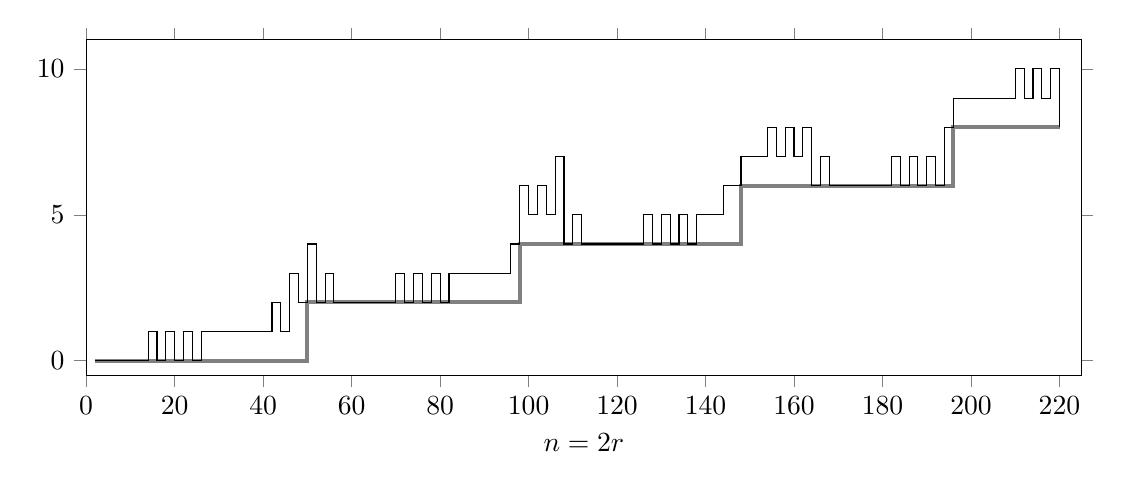
\begin{tikzpicture}
\begin{axis}[width=5.6in,height=2.3in,xmin=0,xmax=225,ymin=-0.5,ymax=11,
xlabel={$n=2r$},axis background/.style={fill=white},tick align=outside]
\addplot[black!50,const plot,line width=1.4pt] coordinates {(2,0)(4,0)(6,0)(8,0)(10,0)(12,0)(14,0)(16,0)(18,0)(20,0)(22,0)(24,0)(26,0)(28,0)(30,0)(32,0)(34,0)(36,0)(38,0)(40,0)(42,0)(44,0)(46,0)(48,0)(50,2)(52,2)(54,2)(56,2)(58,2)(60,2)(62,2)(64,2)(66,2)(68,2)(70,2)(72,2)(74,2)(76,2)(78,2)(80,2)(82,2)(84,2)(86,2)(88,2)(90,2)(92,2)(94,2)(96,2)(98,4)(100,4)(102,4)(104,4)(106,4)(108,4)(110,4)(112,4)(114,4)(116,4)(118,4)(120,4)(122,4)(124,4)(126,4)(128,4)(130,4)(132,4)(134,4)(136,4)(138,4)(140,4)(142,4)(144,4)(146,4)(148,6)(150,6)(152,6)(154,6)(156,6)(158,6)(160,6)(162,6)(164,6)(166,6)(168,6)(170,6)(172,6)(174,6)(176,6)(178,6)(180,6)(182,6)(184,6)(186,6)(188,6)(190,6)(192,6)(194,6)(196,8)(198,8)(200,8)(202,8)(204,8)(206,8)(208,8)(210,8)(212,8)(214,8)(216,8)(218,8)(220,8)};
\addplot[black,const plot,line width=0.4pt] coordinates {(2,0)(4,0)(6,0)(8,0)(10,0)(12,0)(14,1)(16,0)(18,1)(20,0)(22,1)(24,0)(26,1)(28,1)(30,1)(32,1)(34,1)(36,1)(38,1)(40,1)(42,2)(44,1)(46,3)(48,2)(50,4)(52,2)(54,3)(56,2)(58,2)(60,2)(62,2)(64,2)(66,2)(68,2)(70,3)(72,2)(74,3)(76,2)(78,3)(80,2)(82,3)(84,3)(86,3)(88,3)(90,3)(92,3)(94,3)(96,4)(98,6)(100,5)(102,6)(104,5)(106,7)(108,4)(110,5)(112,4)(114,4)(116,4)(118,4)(120,4)(122,4)(124,4)(126,5)(128,4)(130,5)(132,4)(134,5)(136,4)(138,5)(140,5)(142,5)(144,6)(146,6)(148,7)(150,7)(152,7)(154,8)(156,7)(158,8)(160,7)(162,8)(164,6)(166,7)(168,6)(170,6)(172,6)(174,6)(176,6)(178,6)(180,6)(182,7)(184,6)(186,7)(188,6)(190,7)(192,6)(194,8)(196,9)(198,9)(200,9)(202,9)(204,9)(206,9)(208,9)(210,10)(212,9)(214,10)(216,9)(218,10)(220,8)};
\end{axis}
\end{tikzpicture}
\caption{The valuation $v_7(C_r)$ (thin) and the staircase $2E_7(n)$ (thick) for $n=2r\le220$.}\label{figval}
\end{figure}

One question follows from the computation, which is a proof of $v_p(C_r)\ge2E_p(2r)$ for every prime $p\equiv3\pmod4$. The lattice of the archive whose slope contains $\mathrm{gain}_j(p)$ is identified in Section~\ref{sec:gainmech}. It is the lattice $N_u$ of \eqref{Nscale}, a sublattice of the base lattice scaled by an ideal, so $\mathrm{gain}_j(p)$ is an exponent of divisibility of the lifts on that sublattice and is not the exponent of an index.

\section{The interface statements}\label{sec:remain}

Notation as in Sections~\ref{sec:acct} and~\ref{sec:setting}. The geometric core enters the analytic frame through the following statements, which we transcribe from the archive with their names there. They are theorems of the archive, whose proofs Sections~\ref{sec:gainmech} to~\ref{sec:records} reconstruct, and they are not proved in this paper. The letters $C,C'$ are constants, $\ell$ is a power of $\log x$, $n$ is the degree of the cyclotomic field, and $b$ is the size of the nodes.

\medskip\noindent\textbf{R1} (\texttt{LinkMu}). For every $u$ there is a second lattice $N^H_u$ in $N_u\otimes K$ with
\[
\Big|\,\mu(N_u)-\mu(N^H_u)-\sum_w\sigma\Big(w,\sum_{j=1}^m\big(\mathrm{gain}_j(w)+F_j(w)-E_{u,j}(w)\big)\Big)\Big|\le C\,X'' .
\]
Here $\mathrm{gain}_j(w)$ is the number defined by \eqref{gainformula} and $N_u$ is the lattice \eqref{Nscale}.

\noindent\textbf{R2} (\texttt{WordFacts}). For every $u$,
\begin{gather*}
B_u(N_u)\subset R^\vee,\qquad \operatorname{ht}(B_u)\le h_u,\\
\begin{aligned}
\mu(R^\vee)+h_u-\Phi\le{}&\sum_t\big(m\operatorname{ph}(a_t)-ma_t\log\Omega-a_t\log T_u\big)\\
&+C\,N_T\,a\,\ell+C\,m\,(B_0+N_c)\,x^{C'\varepsilon}.
\end{aligned}
\end{gather*}
The archive's statement \texttt{LinkDIV} contains these conditions for every $u$. Among its further conditions are two comparisons between the indices, which read
\[
\Big|\sum_w\sigma\big(w,E_{u,j}(w)\big)-A\log(g_0g_1)\Big|\le C\,B_0,\qquad
\Big|\big(h_u+A\log T_u\big)-\big(h_{u'}+A\log T_{u'}\big)\Big|\le C\,\big(N_T\,a\,\ell+m\,B_0\big),
\]
for all $u$, $u'$ and $1\le j\le m$, with $A=\sum_ta_t$ and with $g_0$, $g_1$ the two primes of Section~\ref{sec:data}.

\noindent\textbf{R3} (\texttt{RestSize}, \texttt{ErrWindows0}, \texttt{BNBounds}, \texttt{GrowthInequalitySizes}). The sizes satisfy
\begin{gather*}
x^{1/2-\varepsilon}\le m\le x^{1/2+\varepsilon/2},\qquad xm\le k\le n^2x^{1/2-\varepsilon},\\
N_T\ge\tfrac12x^{-\varepsilon/8}n,\qquad|T_2|\ge x^{-\varepsilon}n,\qquad a\le2xb,\qquad\Big|\frac{a_t}{b}-x\Big|\le1,\\
B_0\le2\,n\,m\,b\,x^{\varepsilon},\qquad N_c\le\frac{|T_2|\,k\,b\,x^{2\varepsilon}}{n^2} ,
\end{gather*}
where $T_2$ is the set of thick classes of Section~\ref{sec:step5} and $a$ bounds the weights $a_t$. The archive spreads these inequalities over the four statements named above, and its statement \texttt{ChainTied} asks for all of them with one choice of $m$, $k$, $T$ and $T_2$. The archive defines $B_0=2\,n\,m\,b\,x^{\varepsilon}$ and $N_c=|T_2|\,k\,b\,x^{2\varepsilon}/n^2$, so the last two inequalities hold with equality. Its statement \texttt{WinF} asks in addition for $k\le a$, $kb'\le a$, $xnX'\le a$ and $0\le\Lambda_0\le2x^{\varepsilon}$, with $X'$, $b'$ and $\Lambda_0$ as in Section~\ref{sec:host}, and for at most $2^{k-3}$ indices $u$. Proposition~\ref{sizes} shows what these sizes are for.

\noindent\textbf{R4} (\texttt{VWin}, \texttt{LinkN}). For the cyclotomic subfield $E$ and $t_0=\lfloor x^{401}\rfloor$,
\begin{gather*}
V:=\sum_{l}\log l\sum_{1\le e<t_0}\operatorname{length}_{\mathbb Z_l}\Sha_l(E,e)\le\sqrt b,\\
\sum_w\ell_w\,e_w\,\eta_j(w)\le r_j\Big(C\big(f\,m\,b\,\ell^2+N_c\log^2x\big)+V\Big)\qquad(1\le j\le m),
\end{gather*}
with $r_j$ the rank attached to the lift $j$.

\noindent\textbf{R5} (\texttt{HostExW}). For every $0<\varepsilon<\tfrac1{52}$ and every $x$ in a set that contains windows $Y\le x\le Y^{3/2}$ with $Y$ arbitrarily large, there exist the field $E$ and the data of R1 to R4. The field has degree $4n$ with $x^{2+8\varepsilon}\le n\le2x^{2+8\varepsilon}$, its conductor is divisible by $2^{e+2}$ for an integer $e$ with $2^e\le n$ and by two primes $q\equiv3\pmod8$ and $d\equiv7\pmod{16}$ with $q\mid d+1$, every odd prime $p\le Y^{\varepsilon/5}$ divides $d+1$, and the real characters of $E$ of conductor divisible by $q$ or $d$ satisfy $L(\beta,\chi)\ne0$ for $1-\tfrac1{400}<\beta<1$.

\noindent\textbf{R6} (\texttt{ChebyshevInequalityOnWindows}). For a primitive character $\psi$ let $X_\psi$ be a finite set of characters containing $\psi$, with weights $w_\chi>0$. On the windows of R5,
\[
G(x)+\sum_{\chi\in X_\psi,\ \chi\ne1}w_\chi\,G_\chi(x)\le x^{1/2+C\varepsilon}.
\]

\medskip
Given R6 for every $\varepsilon$, Corollary~\ref{corA} gives $\zeta(s)\ne0$ and $L(s,\psi)\ne0$ for $\operatorname{Re}s>\tfrac12$. Proposition~\ref{acct} takes R2 as its hypothesis \eqref{A4}. Its hypothesis \eqref{A2} follows in the archive from R1 and from the statement \texttt{LinkG} of Section~\ref{sec:gainmech}, through the degree formula \eqref{degform}, and R3 gives the balance \eqref{balance}. The archive derives R1 from \texttt{LinkDIV}, and it obtains \texttt{LinkDIV} from the divisibility of the lifts at the inert primes by the route of Section~\ref{sec:gainmech}. Its proof of \texttt{LinkG} does not use that divisibility. The step from the conclusion of Proposition~\ref{acct} to a bound for $G(x)$ is the subject of Section~\ref{sec:point}, which adds a seventh statement R7 and shows in Section~\ref{sec:assembly} that the archive derives R6 from the other six. R4 enters the archive's proof in one place. Its two inequalities together bound the terms $\eta_j(w)$, and that bound is a hypothesis of the archive's proof of \texttt{LinkDIV}, as Section~\ref{sec:archside} records.

\section{From the excess to a bound at a point}\label{sec:point}

The chain bounds a sum over primes sampled at many nodes, and Corollary~\ref{corA} needs a bound for a positive combination of the functions $G_\psi$ at the single point $x$. This section proves the step between the two, first for one quadratic character and then in the generality of the archive, and it shows how the archive assembles its final inequality from that step.

\subsection{The quadratic case}\label{sec:link}

The archive's statement \texttt{GrowthInequalityForm} reads as follows. The classes of the Galois group are of two kinds. A proportion $\delta_2$ of them is thick, with nodes $w$ in $b\le w\le b+\eta+1$, and the others are thin, with nodes $w\le2b'$ where $b'X'\le xb$. The weights satisfy $|a_t/b-x|\le1$. Three further hypotheses concern the functions $G_\psi$ attached to the characters $\psi$ of the Galois group,
\begin{align}
|G_\psi(y)|&\le\theta\,y\qquad\text{for every }\psi\text{ and every }y\ge X'/3,\label{thin}\\
|G_\psi(x)|&\le x^{1/2+\varepsilon}\qquad\text{for three characters }\psi\text{ of order two},\label{valx}\\
\Big|\frac{L'(1,\psi)}{L(1,\psi)}\Big|&\le C\log x\qquad\text{for the same three characters},\label{ellx}
\end{align}
with $2f(x+1)\theta\le1/x$ and $6f(x+1)(\eta+1)\le b/x$. If the excess of the sum over primes above its main term, summed over $t$ and $j$, is at most $\mathrm{Err}$, the conclusion is
\[
N_T\,m\,b\,\frac{\delta_2}2\Big(G(x)-4x^{1/2+\varepsilon}\Big)\le\mathrm{Err}+\frac{2N_Tmb}{x}.
\]
The thick nodes lie within a relative distance $x^{-2}$ of $b$, so every sample point $a_t/w$ lies within a bounded distance of $x$. The following proposition is the quadratic case with thick nodes, and its proof is ours.

\begin{proposition}\label{linkprop}
Let $\chi$ be a real nontrivial Dirichlet character, let $G$ and $G_\chi$ be defined by \eqref{G} and \eqref{Gchi}, and let $B$ and $K$ be constants with $|G(y)|,|G_\chi(y)|\le By$ and $|G(y)-G(y')|,|G_\chi(y)-G_\chi(y')|\le K|y-y'|$ for $y,y'\ge1$. Let $x\ge3$, $b>0$ and $0\le\kappa\le1$, let $a_1,\dots,a_{N_T}$ satisfy $|a_t/b-x|\le1$, and let $w_1,\dots,w_M$ satisfy $b\le w_j\le b(1+\kappa)$. Suppose that
\[
\sum_{t=1}^{N_T}\sum_{j=1}^Mw_j\Big(G\Big(\frac{a_t}{w_j}\Big)-G_\chi\Big(\frac{a_t}{w_j}\Big)\Big)\le\mathrm{Err},
\qquad G_\chi(x)\le V .
\]
Then
\[
G(x)\le V+\frac{\mathrm{Err}}{N_TMb}+2(B+K)\big((x+1)\kappa+1\big).
\]
\end{proposition}
\begin{proof}
Put $D=G-G_\chi$, so $|D(y)|\le2By$ and $|D(y)-D(y')|\le2K|y-y'|$. Fix $t,j$ and put $y=a_t/w_j$. Then $y\le x+1$ and
\[
|y-x|\le\frac{a_t}{b}\Big(1-\frac b{w_j}\Big)+\Big|\frac{a_t}b-x\Big|\le(x+1)\kappa+1 .
\]
Hence
\begin{align*}
\big|w_jD(y)-bD(x)\big|&\le|w_j-b|\,|D(y)|+b\,|D(y)-D(x)|\\
&\le2b(B+K)\big((x+1)\kappa+1\big).
\end{align*}
Summing over $t$ and $j$ gives $N_TMb\,D(x)\le\mathrm{Err}+2N_TMb(B+K)((x+1)\kappa+1)$, and $G(x)=D(x)+G_\chi(x)\le D(x)+V$.
\end{proof}

With $\kappa\le1/x$ the last term is bounded, and the bound for $G(x)$ is $V$ plus the error for one sample of \eqref{balance}. The proposition shows what the link costs. The sum over inert primes controls $G-G_\chi$, and a bound for $G$ needs the separate input $V$, which in the archive is \eqref{valx}. This adds a seventh statement to the list of Section~\ref{sec:remain}.

\medskip\noindent\textbf{R7} (\texttt{ThinScales}, \texttt{ValuesAtX}). For the field of R5, the bounds \eqref{thin}, \eqref{valx} and \eqref{ellx} hold.

\medskip
The characters in \eqref{valx} have conductors built from the primes $q$ and $d$ of R5, which are larger than every power of $x$. For such characters \eqref{valx} is a bound at the single point $x$, and it does not follow from a zero-free half-plane for a fixed $L$-function. Section~\ref{sec:r7} reports how the archive establishes it.

\subsection{The general case}\label{sec:step5}

The definitions of this subsection are read from the archive. Theorem~\ref{step5} is the archive's \texttt{ch\_core} with explicit constants, and the proof is ours.

Let $H$ be a finite abelian group and $\mathcal G=(\mathbb Z/2)^2\times H$, with elements $g=(e_1,e_2,h)$. Put
\begin{gather*}
\Phi=\{g:e_1=0\},\qquad f=|\Phi|=2|H|,\\
p_t(e_1,e_2,h)=(e_1+1,\,e_2+1,\,h+t)\quad(t\in H),
\end{gather*}
so that $p_t$ maps $\mathcal G\setminus\Phi$ onto $\Phi$. Let $A_0$ be a subgroup of $H$ and $T_2$ a nonempty subset of $A_0$, and put $\delta_2=|T_2|/|H|$. For $u_0\in A_0$ call $\rho=(0,e_2,h)\in\Phi$ thick with respect to $u_0$ when $e_2=1$ and $h\in T_2+u_0$. Let $\Psi_0$ be the set of characters $\psi$ of $\mathcal G$ with $\psi(0,0,s)=1$ for every $s\in A_0$, which has $4\,|H/A_0|$ elements. For each character $\psi$ of $\mathcal G$ let $G_\psi\colon(0,\infty)\to\mathbb C$ be a function. For $a>0$, $t\in H$ and a function $w\colon\Phi\to(0,\infty)$ define the excess
\[
\mathrm{De}(a,t,w)=\frac1f\sum_{g\notin\Phi}\ \sum_\psi\overline{\psi(g)}\;w(p_tg)\;G_\psi\Big(\frac a{w(p_tg)}\Big),
\]
where the inner sum runs over the $2f$ characters of $\mathcal G$. In the archive the function attached to the trivial character is $G$, the function $G_\psi$ is the analog of $G_\chi$ for the Dirichlet character attached to $\psi$, and Proposition~\ref{excess} below shows that $\mathrm{De}(a,t,w)$ is the excess of the sum over primes above its main term.

\begin{theorem}[From the excess to a bound at $x$]\label{step5}
With the notation above, let $K\subset\Psi_0$ be a set of characters that contains the trivial character and satisfies $\psi(1,0,0)=1$ for every $\psi\in K$. Let $T\subset H$ have $N_T\ge1$ elements, let $c,\nu\ge0$, and suppose that every $\psi\in K$ that is nontrivial on $\{0\}\times H$ satisfies
\begin{equation}\label{equi}
\Big|\sum_{t\in T}\psi(0,0,t)-c\,N_T\Big|\le\nu\,N_T .
\end{equation}
Put $c_\psi=1$ when $\psi\in K$ is trivial on $\{0\}\times H$ and $c_\psi=c$ for the other $\psi\in K$. Let $x\ge3$, let $b,b',X'>0$ with $b'X'\le xb$, and let $\theta,M\ge0$ and $0\le\eta'\le b$. Let $m\ge1$ be an integer, let $a_t>0$ with $|a_t/b-x|\le1$ for $t\in T$, and for $u_0\in A_0$ and $1\le j\le m$ let $w_{u_0,j}\colon\Phi\to(0,\infty)$ satisfy $b\le w_{u_0,j}(\rho)\le b+\eta'$ when $\rho$ is thick with respect to $u_0$ and $w_{u_0,j}(\rho)\le2b'$ otherwise. Suppose that for every character $\psi$ of $\mathcal G$
\begin{align}
\big|w\,G_\psi(A/w)-w'G_\psi(A/w')\big|&\le\frac{3A\,|w-w'|}{\min(w,w')}&&(A>0,\ 0<w,w'\le A),\label{L1}\\
|G_\psi(y)-G_\psi(x)|&\le M&&(|y-x|\le1),\label{L2}\\
|G_\psi(y)|&\le\theta\,y&&(y\ge X'/3),\label{L3}
\end{align}
and that
\[
\frac1{|A_0|}\sum_{u_0\in A_0}\sum_{t\in T}\sum_{j=1}^m\operatorname{Re}\,\mathrm{De}(a_t,t,w_{u_0,j})\le\mathrm{Err}.
\]
Then
\begin{multline}\label{step5conc}
N_T\,m\,b\,\frac{\delta_2}2\Big(\sum_{\psi\in K}c_\psi\operatorname{Re}G_\psi(x)-\nu\sum_{\psi\in K}|G_\psi(x)|-\sum_{\psi\in\Psi_0\setminus K}|G_\psi(x)|-|\Psi_0|\,M\Big)\\
\le\mathrm{Err}+N_T\,m\Big(2f\theta(x+1)b+6f(x+1)\eta'\Big).
\end{multline}
\end{theorem}
\begin{proof}
Fix $u_0\in A_0$, $t\in T$ and $j$, and write $w=w_{u_0,j}$ and $a=a_t$, so that $(x-1)b\le a\le(x+1)b$. Split the sum over $g\notin\Phi$ in $\mathrm{De}(a,t,w)$ according to whether $p_tg$ is thick with respect to $u_0$.

\emph{Thin classes.} If $p_tg$ is not thick then $w(p_tg)\le2b'$, so $y=a/w(p_tg)$ satisfies
\[
y\ge\frac{(x-1)b}{2b'}\ge\frac{(x-1)X'}{2x}\ge\frac{X'}3 ,
\]
and \eqref{L3} gives $|w(p_tg)\,G_\psi(y)|\le\theta a$. There are $2f$ characters and at most $f$ such $g$, so the thin part of $\mathrm{De}(a,t,w)$ has absolute value at most $2f\theta a\le2f\theta(x+1)b$.

\emph{Thick classes, the nodes.} If $p_tg$ is thick then $b\le w(p_tg)\le b+\eta'\le2b\le a$, and the bound \eqref{L1}, applied with $A=a$ and with $w'=b$, gives the estimate
\[
\Big|w(p_tg)\,G_\psi\Big(\frac a{w(p_tg)}\Big)-b\,G_\psi\Big(\frac ab\Big)\Big|\le\frac{3a\,\eta'}b\le3(x+1)\eta' .
\]
Replacing every thick node by $b$ therefore changes $\mathrm{De}(a,t,w)$ by at most $\frac1f\cdot f\cdot2f\cdot3(x+1)\eta'=6f(x+1)\eta'$.

\emph{Thick classes, the mean over $u_0$.} The class $g=(1,e_2,h)$ has $p_tg=(0,e_2+1,h+t)$, which is thick with respect to $u_0$ exactly when $e_2=0$ and $h=s+u_0-t$ for some $s\in T_2$. Hence for every character $\psi$ of $\mathcal G$
\[
\frac1{|A_0|}\sum_{u_0\in A_0}\ \sum_{\substack{g\notin\Phi\\ p_tg\ \mathrm{thick}}}\overline{\psi(g)}
=\overline{\psi(1,0,0)}\;\psi(0,0,t)\sum_{s\in T_2}\overline{\psi(0,0,s)}\;\frac1{|A_0|}\sum_{u_0\in A_0}\overline{\psi(0,0,u_0)} .
\]
The mean over $u_0$ vanishes when $\psi\notin\Psi_0$ and equals one when $\psi\in\Psi_0$. For $\psi\in\Psi_0$ the sum over $s$ equals $|T_2|$ because $T_2\subset A_0$, and the number $\epsilon_\psi=\psi(1,0,0)$ is $1$ or $-1$ because $(1,0,0)$ has order two. Since $|T_2|/f=\delta_2/2$, the mean over $u_0$ of the thick part of $\mathrm{De}(a_t,t,w_{u_0,j})$ with every thick node replaced by $b$ is
\[
\frac{\delta_2}2\,b\sum_{\psi\in\Psi_0}\epsilon_\psi\,\psi(0,0,t)\,G_\psi\Big(\frac{a_t}b\Big).
\]

\emph{The sum over $t$.} By \eqref{L2}, replacing $G_\psi(a_t/b)$ by $G_\psi(x)$ changes the last display by at most $\frac{\delta_2}2\,b\,|\Psi_0|\,M$. Put $S_\psi=\sum_{t\in T}\psi(0,0,t)$, so $|S_\psi|\le N_T$. For $\psi\in K$ we have $\epsilon_\psi=1$ and, by \eqref{equi}, $|S_\psi-c_\psi N_T|\le\nu N_T$, where the left side vanishes when $\psi$ is trivial on $\{0\}\times H$. Therefore
\[
\operatorname{Re}\sum_{\psi\in\Psi_0}\epsilon_\psi\,S_\psi\,G_\psi(x)\ge N_T\Big(\sum_{\psi\in K}c_\psi\operatorname{Re}G_\psi(x)-\nu\sum_{\psi\in K}|G_\psi(x)|-\sum_{\psi\in\Psi_0\setminus K}|G_\psi(x)|\Big).
\]

\emph{Conclusion.} For each $j$, the four steps give
\begin{multline*}
N_T\,b\,\frac{\delta_2}2\Big(\sum_{\psi\in K}c_\psi\operatorname{Re}G_\psi(x)-\nu\sum_{\psi\in K}|G_\psi(x)|-\sum_{\psi\in\Psi_0\setminus K}|G_\psi(x)|-|\Psi_0|\,M\Big)\\
\le\frac1{|A_0|}\sum_{u_0\in A_0}\sum_{t\in T}\operatorname{Re}\,\mathrm{De}(a_t,t,w_{u_0,j})+N_T\Big(2f\theta(x+1)b+6f(x+1)\eta'\Big),
\end{multline*}
and the sum over $j$ is \eqref{step5conc}.
\end{proof}

The mean over the translations $u_0\in A_0$ removes every character outside $\Psi_0$, and the sum over $t\in T$ gives each character of $K$ a positive weight. For $A_0=H$ and $K=\{1\}$ the set $\Psi_0$ consists of the trivial character and of $\chi_1(g)=(-1)^{e_1}$, $\chi_2(g)=(-1)^{e_2}$ and $\chi_1\chi_2$, and \eqref{step5conc} bounds $\operatorname{Re}G_1(x)$ by the excess plus the three numbers $|G_{\chi_i}(x)|$, as in Proposition~\ref{linkprop}. In the archive $\theta\le1/(2fx^2)$ and $\eta'\le b/(6fx^2)$, so the last bracket of \eqref{step5conc} is at most $2b/x$, and \eqref{L3} is the first half of R7. The archive's statement \texttt{DerivInt} gives \eqref{L2} with $M=\log(x+1)+C_d+|L'(1,\psi)/L(1,\psi)|$ for a constant $C_d$, which is where the third bound \eqref{ellx} of R7 enters.

\subsection{The excess identity}\label{sec:excess}

Theorem~\ref{step5} treats the functions $G_\psi$ as given. This subsection proves the identity that produces them from a sum over primes, which the archive calls \texttt{AskMainBalance}. It extends Proposition~\ref{inert} from one quadratic field to the group $\mathcal G$.

\begin{proposition}[The excess identity]\label{excess}
Let $H$ be a finite abelian group, and let $\mathcal G$, $\Phi$, $f$ and $p_t$ be as in Section~\ref{sec:step5}. For every prime $p$ let $I_p$ be a subgroup of $\mathcal G$ and $\sigma_p$ an element of $\mathcal G$. Let $d$ be a prime and $S$ a finite set of primes with $d\notin S$, and suppose that $I_p=\{0\}$ for $p\notin S\cup\{d\}$, that $I_p\subset\Phi$ and $\sigma_p\in\Phi$ for $p\in S$, and that $I_d=\{0,(1,0,0)\}$. For a character $\psi$ of $\mathcal G$ and a prime power $p^i$ put
\[
\psi(p^i)=\frac1{|I_p|}\sum_{h\in I_p}\psi(i\sigma_p+h),
\]
and put $\psi(n)=0$ for every integer $n\ge1$ that is not a prime power $p^i$ with $i\ge1$. For every nontrivial $\psi$ let $\ell_\psi$ be a complex number and put $G_\psi(y)=\sum_{n\le y}\Lambda(n)\psi(n)(y/n-1)+\ell_\psi y$ for $y>0$, and let $G_\psi$ be the function $G$ when $\psi$ is trivial, where the formula \eqref{G} is used for every $y>0$. Let $\chi_1(g)=(-1)^{e_1}$, and for $i\ge1$ let $g_i$ be the element of the coset $i\sigma_d+I_d$ that does not lie in $\Phi$. Then for every $a>0$, every $t\in H$ and every function $w\colon\Phi\to(0,\infty)$,
\begin{multline*}
2\sum_{\substack{p\notin S\cup\{d\}\\ \sigma_p\notin\Phi}}\log p\sum_{i\ \mathrm{odd}}\max\Big(\frac a{p^i}-w(p_t(i\sigma_p)),0\Big)+\log d\sum_{i\ge1}\max\Big(\frac a{d^i}-w(p_tg_i),0\Big)\\
=a\Big(\log a-1-\gamma+\ell_{\chi_1}-\frac1f\sum_{\rho\in\Phi}\log w(\rho)\Big)+\mathrm{De}(a,t,w).
\end{multline*}
\end{proposition}
\begin{proof}
For $g\notin\Phi$ write $w_g=w(p_tg)$ and $y_g=a/w_g$, and put
\[
A_g=\sum_{n\ge1}\Lambda(n)\,c_g(n)\max\Big(\frac an-w_g,0\Big),\qquad c_g(n)=\frac1{|\mathcal G|}\sum_\psi\overline{\psi(g)}\,\psi(n).
\]
\emph{The left side is $2\sum_{g\notin\Phi}A_g$.} By the orthogonality of the characters, $c_g(p^i)=|I_p|^{-1}$ when $g\in i\sigma_p+I_p$ and $c_g(p^i)=0$ otherwise. For $p\in S$ the coset $i\sigma_p+I_p$ lies in $\Phi$, so these primes do not contribute. For $p\notin S\cup\{d\}$ the coset is the point $i\sigma_p$, which lies outside $\Phi$ exactly when $\sigma_p\notin\Phi$ and $i$ is odd, because $\Phi$ has index two. For $p=d$ the coset $i\sigma_d+I_d$ has two elements, one of which is $g_i\notin\Phi$, and $c_{g_i}(d^i)=\tfrac12$.

\emph{The characters.} Since $|\mathcal G|=2f$ and the terms with $n>y_g$ vanish,
\[
2A_g=\frac1f\sum_\psi\overline{\psi(g)}\;w_g\sum_{n\le y_g}\Lambda(n)\psi(n)\Big(\frac{y_g}n-1\Big).
\]
For nontrivial $\psi$ the inner sum is $G_\psi(y_g)-\ell_\psi y_g$, and for the trivial character it is $G(y_g)+y_g\log y_g-(1+\gamma)y_g$ by \eqref{G}. With $w_gy_g=a$ this gives
\[
2A_g=\frac1f\sum_\psi\overline{\psi(g)}\,w_g\,G_\psi(y_g)+\frac af\Big(\log\frac a{w_g}-1-\gamma\Big)-\frac af\sum_{\psi\ne1}\overline{\psi(g)}\,\ell_\psi .
\]
\emph{The sum over $g$.} The complement of $\Phi$ has $f$ elements and $p_t$ maps it bijectively onto $\Phi$, so the first term sums to $\mathrm{De}(a,t,w)$ and the second to $a(\log a-1-\gamma)-\frac af\sum_{\rho\in\Phi}\log w(\rho)$. The complement of $\Phi$ is a coset of $\Phi$, so $\sum_{g\notin\Phi}\overline{\psi(g)}$ vanishes when $\psi$ is nontrivial on $\Phi$, and it equals $-f$ for $\psi=\chi_1$, which is the nontrivial character that is trivial on $\Phi$. The third term therefore sums to $a\,\ell_{\chi_1}$.
\end{proof}

The identity holds for every choice of the numbers $\ell_\psi$, and the choice $\ell_\psi=L'(1,\psi)/L(1,\psi)$ makes $G_\psi$ the function $G^\ast_\chi$ of Section~\ref{sec:r7} for the primitive Dirichlet character $\chi$ attached to $\psi$. In the archive $S$ consists of $2$ and one further prime, the subgroups $I_p$ are the inertia groups and the $\sigma_p$ are Frobenius elements. The left side is the sum over primes of the route, the first term on the right is the main term of \eqref{acctconc} for one lift, and $\mathrm{De}$ is the excess.

\subsection{The assembly}\label{sec:assembly}

The statement R6 of Section~\ref{sec:remain} is not an independent input. The archive derives it in its theorem \texttt{core\_gm} from three statements, which fit together as follows.

Let $\Xi$ be the finite set of primitive Dirichlet characters whose $L$-functions are the target, which contains the trivial character and is closed under inversion. The archive attaches to $\Xi$ an integer $o\ge1$ and the function
\begin{equation}\label{GXi}
G_\Xi(y)=G(y)+\sum_{\xi\in\Xi,\ \xi\ne1}c_\xi\operatorname{Re}G_\xi(y),\qquad c_\xi=\frac1{3o+1},
\end{equation}
with the exception of at most one real odd character $\xi$, for which $c_\xi=1$. Every weight is positive, so Corollary~\ref{corA} applies to $G_\Xi$. In the setting of Theorem~\ref{step5} the group $H$ comes from the Galois group of the field of R5, the subgroup $A_0$ is chosen with $|\Psi_0|\le4o$, and $K$ is the set of characters of $\mathcal G$ that the archive's definition \texttt{keptA} attaches to $\Xi$. The archive's hypothesis \texttt{CharsA} asks for \eqref{equi} with $c=1/(3o+1)$ and $\nu=4o\,x^{-1+\varepsilon}$, for $|L'(1,\psi)/L(1,\psi)|$ bounded when $\psi\in K$, and for the bound $|L'(1,\psi)/L(1,\psi)|\le C\log x$ on the remaining characters $\psi\in\Psi_0\setminus K$.

The three statements are the following.
\begin{enumerate}
\item (\texttt{ch\_top}) For every $u_0\in A_0$ the excess satisfies $\sum_{t\in T}\sum_{j}\operatorname{Re}\mathrm{De}(a_t,t,w_{u_0,j})\le x^{C\varepsilon}\mathcal B$ with a constant $C\ge0$ and
\[
\mathcal B=N_T\,a\Big(1+\frac{m^2}k\Big)+m\Big(2\,n\,m\,b\,x^{\varepsilon}+\frac{|T_2|\,k\,b\,x^{2\varepsilon}}{n^2}\Big),\qquad n=|H|,
\]
where $a$ is the size of the weights $a_t$ and $k$ is the second size parameter. The archive obtains this bound from the accounting of Section~\ref{sec:acct} and the sizes of R3, and this is the place where R1 to R4 enter.
\item (\texttt{ch\_core}) From the first statement and the sizes of R3, for large $x$,
\[
\sum_{\psi\in K}c_\psi\operatorname{Re}G_\psi(x)\le x^{1/2+(C+3)\varepsilon}+\sum_{\psi\in\Psi_0\setminus K}|G_\psi(x)| .
\]
\item (\texttt{sigA\_le}) Every $\psi\in\Psi_0\setminus K$ satisfies $|G_\psi(x)|\le x^{1/2+\varepsilon}$, which is R7.
\end{enumerate}
The left side of the second statement is $G_\Xi(x)$, and the three statements give $G_\Xi(x)\le x^{1/2+(C+3)\varepsilon}+4o\,x^{1/2+\varepsilon}$, which is at most $x^{1/2+(C+4)\varepsilon}$ once $x^{\varepsilon}\ge1+4o$. This is R6 on the windows where the data of R5 exist.

The second statement follows from Theorem~\ref{step5} and from the sizes that the archive collects under the names \texttt{RestSize}, \texttt{SizesA} and \texttt{CostWindows}. The next two results prove this, and the proofs are ours.

\begin{proposition}[The arithmetic of the sizes]\label{sizes}
Let $x\ge3$, $\varepsilon>0$ and $C\ge0$, let $n,N_T,N_2,m\ge1$ be integers and $a,b,k>0$ real numbers, and suppose that
\begin{gather}
a\le2xb,\qquad N_T\ge\tfrac12x^{-\varepsilon/8}\,n,\qquad x^{-\varepsilon}n\le N_2\le n,\label{sz1}\\
x^{1/2-\varepsilon}\le m\le x^{1/2+\varepsilon/2},\qquad xm\le k\le n^2x^{1/2-\varepsilon},\qquad x^{3\varepsilon/8}\ge26.\label{sz2}
\end{gather}
Put $\delta_2=N_2/n$ and
\[
\mathcal B=N_T\,a\Big(1+\frac{m^2}k\Big)+m\Big(2\,n\,m\,b\,x^{\varepsilon}+\frac{N_2\,k\,b\,x^{2\varepsilon}}{n^2}\Big).
\]
Then
\[
x^{C\varepsilon}\,\mathcal B\le\frac{10}{13}\,x^{1/2+(C+3)\varepsilon}\cdot N_T\,m\,b\,\frac{\delta_2}2 .
\]
\end{proposition}
\begin{proof}
Divide $\mathcal B$ by $N_Tmb\,\delta_2/2$ and bound the three terms with \eqref{sz1} and \eqref{sz2}. In the first term $m/k\le1/x$ and $1/\delta_2\le x^{\varepsilon}$, so that
\[
\frac{2a}{m\,b\,\delta_2}\Big(1+\frac{m^2}k\Big)=\frac{2a}{b\,\delta_2}\Big(\frac1m+\frac mk\Big)\le4x^{1+\varepsilon}\Big(x^{-1/2+\varepsilon}+\frac1x\Big)=4x^{1/2+2\varepsilon}+4x^{\varepsilon}.
\]
Since $n/N_T\le2x^{\varepsilon/8}$,
\[
\frac{2m\cdot2\,n\,m\,b\,x^{\varepsilon}}{N_T\,m\,b\,\delta_2}=\frac{4\,n\,m\,x^{\varepsilon}}{N_T\,\delta_2}\le8\,x^{1/2+21\varepsilon/8}.
\]
Since $N_2/\delta_2=n$ and $k\le n^2x^{1/2-\varepsilon}$,
\[
\frac{2m\,N_2\,k\,b\,x^{2\varepsilon}}{n^2\,N_T\,m\,b\,\delta_2}=\frac{2\,k\,x^{2\varepsilon}}{n\,N_T}\le\frac{2\,n\,x^{1/2+\varepsilon}}{N_T}\le4\,x^{1/2+9\varepsilon/8}.
\]
Each of the four bounds is at most its coefficient times $x^{1/2+21\varepsilon/8}$, so
\[
\frac{\mathcal B}{N_T\,m\,b\,\delta_2/2}\le20\,x^{1/2+21\varepsilon/8}=20\,x^{-3\varepsilon/8}\,x^{1/2+3\varepsilon}\le\frac{20}{26}\,x^{1/2+3\varepsilon}.\qedhere
\]
\end{proof}

\begin{corollary}[The second statement of the assembly]\label{asm}
Suppose that the hypotheses of Theorem~\ref{step5} hold, and that the hypotheses of Proposition~\ref{sizes} hold with $n=|H|$ and $N_2=|T_2|$. Suppose further that
\begin{gather*}
\mathrm{Err}\le x^{C\varepsilon}\,\mathcal B,\qquad2f(x+1)\theta\le\frac1x,\qquad6f(x+1)\eta'\le\frac bx,\\
4x^{\varepsilon-1}+\nu\sum_{\psi\in K}|G_\psi(x)|+|\Psi_0|\,M\le\frac3{13}\,x^{1/2+(C+3)\varepsilon}.
\end{gather*}
Then
\[
\sum_{\psi\in K}c_\psi\operatorname{Re}G_\psi(x)\le x^{1/2+(C+3)\varepsilon}+\sum_{\psi\in\Psi_0\setminus K}|G_\psi(x)| .
\]
\end{corollary}
\begin{proof}
Divide \eqref{step5conc} by $N_Tmb\,\delta_2/2$. Proposition~\ref{sizes} bounds the term with $\mathrm{Err}$ by $\tfrac{10}{13}x^{1/2+(C+3)\varepsilon}$. The two conditions on $\theta$ and $\eta'$ bound the last bracket of \eqref{step5conc} by $2b/x$, and $2b/x$ divided by $b\,\delta_2/2$ is $4/(x\delta_2)\le4x^{\varepsilon-1}$. The last hypothesis bounds this term together with the terms of \eqref{step5conc} that contain $\nu$ and $M$ by $\tfrac3{13}x^{1/2+(C+3)\varepsilon}$.
\end{proof}

The last hypothesis of Corollary~\ref{asm} holds for large $x$ in the setting of the archive. There $\nu=4o\,x^{-1+\varepsilon}$ and $|G_\psi(x)|\le Bx$ by the bound of Section~\ref{sec:functions}, so the term with $\nu$ is $O(x^{\varepsilon})$, and $M$ is at most a constant times $\log x$. The proof of Proposition~\ref{sizes} also shows where the square root comes from. After division the bracket $\mathcal B$ has the four shapes
\[
\frac xm,\qquad\frac{xm}k,\qquad m\,x^{c\varepsilon},\qquad\frac{k\,x^{c\varepsilon}}{n\,N_T},
\]
the first three of which are the shapes of \eqref{balance}. The first and the third balance at $m=\sqrt x$, the second is at most one because $xm\le k$, and the fourth is at most $x^{1/2+c\varepsilon}$ because $k\le n^2x^{1/2-\varepsilon}$. The two conditions on $k$ are compatible when $n^2\ge x^{1/2+\varepsilon}m$, and with $m\ge x^{1/2-\varepsilon}$ this asks for a group $H$ with at least $\sqrt x$ elements.

The archive asks for the bounds of R7 for the products $\xi\,(\tfrac{\cdot}{q})^i(\tfrac{\cdot}{d})^j$ with $(i,j)\ne(0,0)$ and $\xi$ a character of a fixed modulus. This is the description of $\Psi_0\setminus K$ as the products of the characters of $K$ with the quadratic characters of the auxiliary primes $q$ and $d$. The construction of the host field makes the identification, since every frame character outside the kept set has a primitive character that induces $\xi\,(\tfrac{\cdot}{q})^i(\tfrac{\cdot}{d})^j$ with $(i,j)\ne(0,0)$, by the size lemmas behind the host (Section~\ref{sec:host}). Section~\ref{sec:r7} takes up that statement.

\section{The auxiliary primes}\label{sec:r7}

In the archive the three characters of R7 are $n\mapsto(\tfrac{-q}{n})$, $n\mapsto(\tfrac{-d}{n})$ and their product, twisted by the characters $\xi$ of a fixed modulus $N_0$. Since $q\equiv d\equiv3\pmod4$, these are $n\mapsto(\tfrac nq)$ and $n\mapsto(\tfrac nd)$ on odd $n$. The two primes are taken in the ranges
\[
\tfrac12Y^{\varepsilon/5}<\log q\le Y^{\varepsilon/5},\qquad \tfrac12z'<\log d\le z',\qquad Y^{\varepsilon/5}\log^2Y\le z'\le K^2\,Y^{\varepsilon/5}\log^2Y,
\]
with $q\equiv3\pmod8$, $d\equiv7\pmod{16}$ and $d\equiv-1$ modulo $q$ and modulo every odd prime $p\le Y^{\varepsilon/5}$. The bounds \eqref{valx} and \eqref{ellx} are required for every $y$ with $Y\le y\le Y^K$. The archive proves the existence of such $q$ and $d$ in two stages. Its theorem \texttt{stage1} says that all candidates $q$ outside a proportion $\eta$ are good, for every $\eta>0$, and \texttt{stage2} says the same for the candidates $d$ once a good $q$ is fixed.

This section proves both stages and the bound \eqref{thin} from statements on the zeros of Dirichlet $L$-functions and on primes in progressions, which Section~\ref{sec:classical} lists. Seven of them are classical and are quoted with references, and one is quoted from the archive. The proofs of this section are ours, and we did not compare them with the proofs of the archive.

For a Dirichlet character $\chi$ put $\psi(u,\chi)=\sum_{n\le u}\Lambda(n)\chi(n)$ and $\psi(u)=\sum_{n\le u}\Lambda(n)$. For a primitive character $\chi$ modulo $N\ge3$ and $y\ge1$ put
\[
G^\ast_\chi(y)=\sum_{n\le y}\Lambda(n)\chi(n)\Big(\frac yn-1\Big)+\frac{L'(1,\chi)}{L(1,\chi)}\,y ,
\]
so that the function of \eqref{Gchi} is $G_\chi=\operatorname{Re}G^\ast_\chi$ and $|G_\chi(y)|\le|G^\ast_\chi(y)|$.

\subsection{Classical statements}\label{sec:classical}

We use the following eight statements, in which every constant is absolute. A zero of $L(s,\chi)$ means a zero in the strip $0<\operatorname{Re}s<1$, the number of zeros $\rho$ with $\operatorname{Re}\rho\ge\sigma$ and $|\operatorname{Im}\rho|\le T$ is $N(\sigma,T,\chi)$, and $\operatorname{li}(X)=\int_2^Xdt/\log t$.
\begin{enumerate}
\item[(C1)] Chebyshev \cite{chebyshev}. There is $c_0\ge1$ with $\psi(u)\le c_0u$ and $\pi(u)\log u\le c_0u$ for every $u\ge1$.
\item[(C2)] The prime number theorem for characters \cite[Theorem~5.27]{ik}, \cite[Ch.~20]{davenport}. There are $0<c_1\le\tfrac12$ and $C_1\ge1$ such that for every primitive character $\chi$ modulo $N\ge3$ and every $u\ge2$
\[
\Big|\psi(u,\chi)+\frac{u^{\beta}}{\beta}\Big|\le C_1\,u\,(\log N)^4\exp\Big(-\frac{c_1\log u}{\sqrt{\log u}+\log N}\Big),
\]
where the term with $\beta$ is present when $\chi$ is real and $L(s,\chi)$ has a real zero $\beta>1-c_1/\log N$, and is absent otherwise. Moreover $|\psi(u)-u|\le C_1u\exp(-c_1\sqrt{\log u})$ for $u\ge2$, and the series $\sum_n\Lambda(n)\chi(n)/n$ converges to $-L'(1,\chi)/L(1,\chi)$.
\item[(C3)] Page \cite{page}, \cite[Ch.~14]{davenport}. There is $c_2>0$ such that for every $R\ge3$ at most one primitive real character of conductor at most $R$ has a real zero $\beta>1-c_2/\log R$.
\item[(C4)] Zeros and the explicit formula \cite[Ch.~16 and~19]{davenport}. Let $\chi$ be a primitive character modulo $N\ge3$. The map $\rho\mapsto1-\bar\rho$ permutes the zeros of $L(s,\chi)$, and for every real $t$ the number of zeros with $|\operatorname{Im}\rho-t|\le1$ is at most $C_2\log(N(|t|+2))$. For $2\le T\le u$,
\[
\Big|\psi(u,\chi)+\frac{u^{\beta_1}}{\beta_1}+\sum_{|\operatorname{Im}\rho|<T}\frac{u^\rho}{\rho}\Big|\le C_2\Big(\frac{u\log^2(Nu)}T+u^{1/4}\log u\Big),
\]
where the term with $\beta_1$ is present when the zero $\beta$ of (C2) exists, and then $\beta_1=\beta$ and the sum omits $\beta_1$ and $1-\beta_1$.
\item[(C5)] Montgomery's density theorem \cite[Theorem~12.2]{montgomerytopics}. There is $C_3$ such that for $Q,T\ge2$ and $\tfrac45\le\sigma\le1$
\[
\sum_{N\le Q}\ \sum_{\chi}N(\sigma,T,\chi)\le C_3\,(Q^2T)^{5(1-\sigma)/2}\log^{14}(QT),
\]
where the inner sum runs over the primitive characters modulo $N$.
\item[(C6)] Primes in the class $3$ modulo $8$ \cite[Ch.~20]{davenport}. There is $U_0$ such that for $U\ge U_0$ the number of primes $q\equiv3\pmod8$ with $\sqrt U<q\le U$ is at least $U/(5\log U)$.
\item[(C7)] Primes in progressions of large modulus. There are $c_6>0$, $A_0$ and $C_0$ with the following property. For every integer $M$ divisible by $8$, consider the pairs $(\chi_1,\beta_1)$ in which $\chi_1$ is a real nonprincipal character modulo $M$ and $\beta_1$ is a real zero of $L(s,\chi_1)$ with $1-1/(8\log M)<\beta_1<1$. If such pairs exist, one of them can be chosen so that the following estimate holds with the chosen pair, and if such pairs do not exist the estimate holds with the second form of the main term. For every $X\ge2$ with $C_0\log M\cdot\log(\log M+2)\le\log X$ and every $b$ coprime to $M$, the number $\pi(X;M,b)$ of primes $p\le X$ with $p\equiv b\pmod M$ satisfies
\[
\big|\pi(X;M,b)-\mathfrak m(X;M,b)\big|\le A_0\Big(e^{-c_6\log X/\log M}+e^{-\sqrt{c_6\log X}}\Big)\,\mathfrak m(X;M,b),
\]
where $\mathfrak m(X;M,b)=\big(\operatorname{li}(X)-\chi_1(b)\operatorname{li}(X^{\beta_1})\big)/\varphi(M)$ for the chosen pair and $\mathfrak m(X;M,b)=\operatorname{li}(X)/\varphi(M)$ when such pairs do not exist.
\item[(C8)] The distance of a real zero from $1$ \cite[Ch.~14]{davenport}. There is $0<c_7\le1$ such that every real zero $\beta$ of $L(s,\chi)$, for a real nonprincipal character $\chi$ modulo $M\ge3$, satisfies $\beta\le1-c_7/(M^{1/2}\log^2M)$.
\end{enumerate}
The statement (C7) is the archive's \texttt{PNTAPRelW}, and the archive has a proof of it that we did not read. Its error term is relative to a main term that contains the exceptional zero, which is the form that the theorems of Linnik and of Gallagher \cite{gallagher} take once the repulsion of the other zeros by an exceptional zero is used. We did not find (C7) in this exact form in the literature, but it follows from Gallagher's prime number theorem \cite[Theorem~7]{gallagher} by partial summation. In the form in which later expositions record it, that theorem gives the sum of $\log p$ over the primes $p\le X$ in a class modulo $q$ with a relative error $O(e^{-c\log X/\log R})$, uniformly for $q\le R$ and $e^{\sqrt{\log X}}\le R\le X^{c'}$, with the exceptional zero in the main term. With $R=\max(M,e^{\sqrt{\log X}})$ this is the error of (C7), and the hypothesis $C_0\log M\log(\log M+2)\le\log X$ gives $R\le X^{c'}$ when $C_0$ is large. A real zero that lies in one of the two exceptional ranges and not in the other contributes $O(X^{\beta_1-1})$ relative to the main term, which is absorbed after $c_6$ is reduced. We have not compared this derivation line by line with Gallagher's paper.

\begin{lemma}[A bound under a zero-free box]\label{boxpsi}
Let $\chi$ be a primitive character modulo $N\ge3$ and let $Q\ge2$. Suppose that $L(s,\chi)\ne0$ for every $s$ with $\operatorname{Re}s>1-\tfrac1{400}$ and $|\operatorname{Im}s|\le Q$. Then for every $u\ge2$ and every $T$ with $2\le T\le\min(u,Q)$
\[
|\psi(u,\chi)|\le C_4\Big(u^{1-1/400}\log^2(NT)+\frac{u\log^2(Nu)}T\Big),
\]
with an absolute constant $C_4$.
\end{lemma}
\begin{proof}
Let $\rho=\beta+i\gamma$ be a zero with $|\gamma|<T$. Then $\beta\le1-\tfrac1{400}$ by hypothesis, and the same bound for the zero $1-\bar\rho$ gives $\beta\ge\tfrac1{400}$, so $|u^\rho/\rho|\le u^{1-1/400}/\max(\tfrac1{400},|\gamma|)$. By the count of zeros in (C4),
\[
\sum_{|\gamma|<T}\frac1{\max(\frac1{400},|\gamma|)}\le400\,C_2\log(3N)+\sum_{1\le k\le T}\frac{2C_2\log(N(k+3))}{k}\le C\log^2(NT).
\]
If the term with $\beta_1$ is present then $\tfrac12\le\beta_1\le1-\tfrac1{400}$ and $u^{\beta_1}/\beta_1\le2u^{1-1/400}$. Finally $u^{1/4}\log u\le Cu^{1-1/400}$, and the explicit formula of (C4) gives the claim.
\end{proof}

\subsection{Identities}

\begin{lemma}\label{gchisplit}
Let $\chi$ be a primitive character modulo $N\ge3$, and let $1\le y\le y'\le Z$. Then
\begin{align}
G^\ast_\chi(y)&=-\psi(y,\chi)-y\sum_{n>y}\frac{\Lambda(n)\chi(n)}{n}=-y\int_y^\infty\frac{\psi(u,\chi)}{u^2}\,du,\label{id1}\\
G^\ast_\chi(y)&=-S_Z(y)-y\,T_Z,\label{id2}\\
\frac{S_Z(y')}{y'}-\frac{S_Z(y)}{y}&=-\int_y^{y'}\frac{\psi(u,\chi)}{u^2}\,du,\label{id3}
\end{align}
where
\[
S_Z(y)=\sum_{n\le Z}\Lambda(n)\chi(n)\min\Big(1,\frac yn\Big),\qquad T_Z=\sum_{n>Z}\frac{\Lambda(n)\chi(n)}{n}=-\frac{\psi(Z,\chi)}{Z}+\int_Z^\infty\frac{\psi(u,\chi)}{u^2}\,du .
\]
The identity \eqref{id3} holds with $\Lambda(n)\chi(n)$ replaced by arbitrary complex coefficients in $S_Z$ and in $\psi$. Moreover $G(y)=-y\int_y^\infty(\psi(u)-u)\,u^{-2}\,du$ for the function $G$ of \eqref{G}.
\end{lemma}
\begin{proof}
By (C2) the series $\sum_n\Lambda(n)\chi(n)/n$ converges to $-L'(1,\chi)/L(1,\chi)$, so
\[
G^\ast_\chi(y)=y\sum_{n\le y}\frac{\Lambda(n)\chi(n)}n-\psi(y,\chi)-y\sum_{n\ge1}\frac{\Lambda(n)\chi(n)}n ,
\]
which is the first equality of \eqref{id1}. For $V>y$, summation by parts gives
\begin{equation}\label{parts}
\sum_{y<n\le V}\frac{\Lambda(n)\chi(n)}n=\frac{\psi(V,\chi)}V-\frac{\psi(y,\chi)}y+\int_y^V\frac{\psi(u,\chi)}{u^2}\,du .
\end{equation}
By (C2), $\psi(V,\chi)/V$ tends to zero as $V\to\infty$ and the integral converges, which gives the second equality of \eqref{id1} and, with $y=Z$, the formula for $T_Z$. Splitting the sum over $n>y$ at $Z$ gives \eqref{id2}, because $\min(1,y/n)$ equals $1$ for $n\le y$ and $y/n$ for $y<n\le Z$. The same splitting and \eqref{parts} with $V=Z$ give
\[
\frac{S_Z(y)}y=\frac{\psi(y,\chi)}y+\sum_{y<n\le Z}\frac{\Lambda(n)\chi(n)}n=\frac{\psi(Z,\chi)}Z+\int_y^Z\frac{\psi(u,\chi)}{u^2}\,du ,
\]
and the difference of this identity at $y'$ and at $y$ is \eqref{id3}. This step is a summation by parts and holds for arbitrary coefficients. For $G$, the same summation by parts gives $\sum_{n\le y}\Lambda(n)/n=\psi(y)/y+\int_1^y\psi(u)u^{-2}du$, and (C2) together with the expansion of $\zeta'/\zeta$ at $s=1$ gives $\int_1^\infty(\psi(u)-u)u^{-2}du=-1-\gamma$. Hence
\[
y\sum_{n\le y}\frac{\Lambda(n)}n-\psi(y)=y\log y-(1+\gamma)y-y\int_y^\infty\frac{\psi(u)-u}{u^2}\,du ,
\]
and \eqref{G} gives the claim.
\end{proof}

\subsection{The thin scales}

\begin{proposition}[Decay of $G^\ast_\chi$ at large scales]\label{thinprop}
Let $\chi$ be a primitive character modulo $N\ge3$, let $\lambda\ge\max(1,\log N)$ and $0<c_\ast\le\tfrac12$, and suppose that either $\chi$ is not real, or $L(\beta,\chi)\ne0$ for every real $\beta$ with $1-c_\ast<\beta<1$. Then for every $y\ge2$, with $t_0=\log y$,
\[
\frac{|G^\ast_\chi(y)|}{y}\le\frac{2e^{-c_\ast t_0}}{c_\ast}+C_1\lambda^4\Big(\frac{2\lambda}{c_1}\,e^{-c_1t_0/(2\lambda)}+\frac8{c_1^2}\Big(1+\frac{c_1\sqrt{t_0}}2\Big)e^{-c_1\sqrt{t_0}/2}\Big).
\]
\end{proposition}
\begin{proof}
If the term with $\beta$ in (C2) is present then $\tfrac12\le\beta\le1-c_\ast$, so $u^\beta/\beta\le2u^{1-c_\ast}$. Since $\log N\le\lambda$, the bound of (C2) gives, for every $u\ge2$,
\[
|\psi(u,\chi)|\le2u^{1-c_\ast}+C_1\,u\,\lambda^4\exp\Big(-\frac{c_1\log u}{\sqrt{\log u}+\lambda}\Big).
\]
For $t>0$ the quotient $t/(\sqrt t+\lambda)$ is at least $\sqrt t/2$ when $\sqrt t\ge\lambda$ and at least $t/(2\lambda)$ otherwise, so the exponential is at most $e^{-c_1t/(2\lambda)}+e^{-c_1\sqrt t/2}$ with $t=\log u$. By \eqref{id1} and the substitution $u=e^t$,
\[
\frac{|G^\ast_\chi(y)|}y\le\int_y^\infty\frac{2\,du}{u^{1+c_\ast}}+C_1\lambda^4\int_{t_0}^\infty\Big(e^{-c_1t/(2\lambda)}+e^{-c_1\sqrt t/2}\Big)dt ,
\]
and the three integrals are $2y^{-c_\ast}/c_\ast$, $(2\lambda/c_1)e^{-c_1t_0/(2\lambda)}$ and $(8/c_1^2)(1+c_1\sqrt{t_0}/2)e^{-c_1\sqrt{t_0}/2}$.
\end{proof}

In the archive the characters of the field of R5 have $\log N\le Ax^{\varepsilon/5}\log^2x$, and \eqref{thin} is asked for $y\ge\tfrac13\exp(x^{\varepsilon/3})$. With $\lambda=Ax^{\varepsilon/5}\log^2x$ and $t_0\ge\tfrac12x^{\varepsilon/3}$ the two exponents $c_1t_0/(2\lambda)$ and $c_1\sqrt{t_0}/2$ exceed $2x^{\varepsilon/8}$ for large $x$, because $\tfrac13-\tfrac15>\tfrac18$ and $\tfrac16>\tfrac18$, and the factors in front are powers of $x$. Proposition~\ref{thinprop} therefore gives \eqref{thin} with $\theta=\exp(-x^{\varepsilon/8})$ for large $x$, under the hypothesis on real zeros. For the trivial character the last identity of Lemma~\ref{gchisplit} and the second bound of (C2) give the same decay for $G$. The hypothesis on real zeros is part of R5 for the real characters whose conductor is divisible by $q$ or $d$, and for the finitely many characters of conductor dividing $N_0$ it holds with a constant $c_\ast$ that depends on $N_0$.

\subsection{A mean square over prime moduli}

\begin{proposition}[Mean square with exceptional classes]\label{meansq}
Let $Z\ge1$ and $\eta\ge0$, let $P$ be a finite set of primes $q>Z$, let $E$ be a finite set of squarefree integers $s>1$, and let $c_n$ for $1\le n\le Z$ be complex numbers. Suppose that $\big|\sum_{q\in P}(\tfrac sq)\big|\le\eta\,|P|$ for every squarefree integer $s$ with $1<s\le Z^2$ and $s\notin E$. Then
\[
\sum_{q\in P}\Big|\sum_{n\le Z}c_n\Big(\frac nq\Big)\Big|^2\le|P|\Big(\sum_{\substack{n,n'\le Z\\ nn'\ \mathrm{a\ square}}}|c_nc_{n'}|+\sum_{s\in E}\ \sum_{\substack{n,n'\le Z\\ nn'/s\ \mathrm{a\ square}}}|c_nc_{n'}|+\eta\Big(\sum_{n\le Z}|c_n|\Big)^2\Big).
\]
\end{proposition}
\begin{proof}
Expanding the square gives $\sum_{n,n'}c_n\overline{c_{n'}}\sum_{q\in P}(\tfrac{nn'}q)$. Each $q\in P$ exceeds $Z$, so $q$ does not divide $nn'$. Write $nn'=sr^2$ with $s$ squarefree, so that $s\le Z^2$ and the symbol equals $(\tfrac sq)$. If $s=1$ the inner sum is $|P|$, if $s\in E$ it has absolute value at most $|P|$, and otherwise it has absolute value at most $\eta|P|$.
\end{proof}

In both stages the sum of the symbols $(\tfrac sq)$ over the candidates is small for most squarefree $s$, and it is large for the $s$ in a set of the following kind. For $z\ge2$ and an integer $s^\ast\ge1$ without prime factors $p\le z$, let $\mathcal S(z,s^\ast)$ be the set of squarefree integers $s>1$ with the following property. The largest divisor of $s$ without prime factors $p\le z$ equals $1$ or $s^\ast$.

\begin{lemma}[The coefficients]\label{coef}
Let $3\le y\le Z$, let $\kappa(n)$ be complex numbers with $|\kappa(n)|\le1$, and put $c_n=\Lambda(n)\kappa(n)\min(1,y/n)$ for $n\le Z$. Let $z\ge2$ with $z\log y\le\sqrt y$, and let $s^\ast\ge1$ be an integer without prime factors $p\le z$. With the constant $c_0$ of \textup{(C1)},
\begin{align*}
\sum_{\substack{n,n'\le Z\\ nn'\ \mathrm{a\ square}}}|c_nc_{n'}|&\le60\,c_0^2\,y\log y,\\
\sum_{s\in\mathcal S(z,s^\ast)}\ \sum_{\substack{n,n'\le Z\\ nn'/s\ \mathrm{a\ square}}}|c_nc_{n'}|&\le81\,c_0^2\,y,\\
\sum_{n\le Z}|c_n|&\le3\,c_0\,y\log Z .
\end{align*}
\end{lemma}
\begin{proof}
For a prime $p$ put $W_p=\sum_{a\ge1}\log p\,\min(1,y/p^a)$, and put $W_\square=\sum_m\Lambda(m)\min(1,y/m^2)$, which bounds the sum of $|c_n|$ over the squares $n$.

If $p\le y$, the powers $p^a\le y$ contribute at most $\log y$ to $W_p$, and the powers $p^a>y$ contribute at most $2\log p$, because the numbers $y/p^a$ are less than one and decrease by the factor $p\ge2$. If $p>y$ then $W_p\le2y\log p/p\le2\log y$. Hence $W_p\le3\log y$ for every $p$, and by (C1)
\[
\sum_{p\le y}W_p^2\le9\,\pi(y)\log^2y\le9c_0\,y\log y .
\]
For $p>y$ we group the primes in the intervals $2^ky<p\le2^{k+1}y$ and use (C1) again,
\[
\sum_{p>y}W_p^2\le4y^2\sum_{k\ge0}\pi(2^{k+1}y)\,\frac{\log^2(2^{k+1}y)}{4^ky^2}\le8c_0\,y\sum_{k\ge0}\frac{\log y+(k+1)\log2}{2^k}\le40c_0\,y\log y ,
\]
since $\sum_k2^{-k}=2$, $\sum_k(k+1)2^{-k}=4$ and $4\log2\le3\log y$. By (C1) and a summation by parts,
\[
W_\square\le\psi(\sqrt y)+y\sum_{m>\sqrt y}\frac{\Lambda(m)}{m^2}\le c_0\sqrt y+2y\int_{\sqrt y}^\infty\frac{\psi(u)}{u^3}\,du\le3c_0\sqrt y .
\]
Let $n=p^a$ and $n'=p'^{\,b}$ be prime powers. If $nn'$ is a square then either $p=p'$, or $n$ and $n'$ are both squares, so the first sum is at most $\sum_pW_p^2+W_\square^2\le49c_0y\log y+9c_0^2y$.

For the second sum, write $nn'=sr^2$ with $s>1$ squarefree, so that the prime factors of $s$ are the primes that occur in $nn'$ to an odd power. Let $\mathcal A$ be the set of the $n\le Z$ that are squares or powers of a prime $p\le z$. The sum of $|c_n|$ over $\mathcal A$ is at most
\[
W_\square+\sum_{p\le z}W_p\le3c_0\sqrt y+3z\log y\le6c_0\sqrt y .
\]
If every prime factor of $s$ is at most $z$, then $n$ and $n'$ both lie in $\mathcal A$, because a prime $p>z$ that occurs in $n$ to an odd power must occur in $n'$ to an odd power, and then $nn'$ is a square. These pairs contribute at most $36c_0^2y$. Otherwise $s\in\mathcal S(z,s^\ast)$ means that the primes $p>z$ dividing $s$ are the prime factors of $s^\ast$, and $nn'$ has at most two prime factors. If $s^\ast$ is a prime $p^\ast$, then one of $n$, $n'$ is an odd power of $p^\ast$ and the other lies in $\mathcal A$, which contributes at most $2W_{p^\ast}\cdot6c_0\sqrt y\le36c_0\sqrt y\log y$. If $s^\ast$ is a product of two primes, then $n$ and $n'$ are odd powers of these primes, which contributes at most $18\log^2y$. The integer $s^\ast$ is fixed, so at most one of the last two cases occurs, and $18\log^2y\le36c_0\sqrt y\log y\le36c_0^2y$ because $\log y\le\sqrt y$ and $c_0\ge1$. The second sum is therefore at most $36c_0^2y+36c_0^2y=72c_0^2y$. Finally, by (C1) and a summation by parts,
\[
\sum_{n\le Z}|c_n|\le\psi(y)+y\sum_{y<n\le Z}\frac{\Lambda(n)}n\le c_0y+y\Big(c_0+c_0\log\frac Zy\Big)\le3c_0\,y\log Z .\qedhere
\]
\end{proof}

\subsection{Uniformity on a window}

A mean square bounds a sum at one point $y$ for most $q$, and R7 asks for all $y$ in $Y\le y\le Y^K$. The identity \eqref{id3} controls a whole dyadic block by its left endpoint and by one integral.

\begin{proposition}[A window from dyadic blocks]\label{window}
Let $0<\tau\le\tfrac12$, $8\le Y\le X$ and $Z\ge2X$, and let $\eta\ge0$ with $\eta\,X\log^2Z\le1$. Let $z\ge2$ with $z\log Y\le\sqrt Y$, and let $s^\ast\ge1$ be an integer without prime factors $p\le z$. Let $P$ be a finite set of primes $q>Z$, and suppose that $\big|\sum_{q\in P}(\tfrac sq)\big|\le\eta|P|$ for every squarefree $s$ with $1<s\le Z^2$ and $s\notin\mathcal S(z,s^\ast)$. Let $|\kappa(n)|\le1$, and for $q\in P$ put
\[
S_q(y)=\sum_{n\le Z}\Lambda(n)\kappa(n)\Big(\frac nq\Big)\min\Big(1,\frac yn\Big).
\]
Then the number of $q\in P$ for which $|S_q(y)|>\tfrac12y^{1/2+\tau}$ for some $y$ with $Y\le y\le X$ is at most
\[
\frac{16000\,c_0^2}{(1-4^{-\tau})^2}\;|P|\;Y^{-2\tau}\log(2Y).
\]
\end{proposition}
\begin{proof}
Put $\psi_q(u)=\sum_{n\le u}\Lambda(n)\kappa(n)(\tfrac nq)$. The function $\sqrt y/\log y$ increases for $y\ge8$, so $z\log y\le\sqrt y$ for every $y\ge Y$. For $Y\le y\le2X$, Proposition~\ref{meansq} with the set $E$ of the $s\le Z^2$ in $\mathcal S(z,s^\ast)$ and Lemma~\ref{coef} give
\[
\sum_{q\in P}|S_q(y)|^2\le|P|\,c_0^2\Big(60\,y\log y+81\,y+9\,\eta\,y^2\log^2Z\Big)\le159\,c_0^2\,|P|\,y\log y ,
\]
because $\eta y^2\log^2Z\le2y$. The same results with $Z$ replaced by $u$ and $y=u$ give $\sum_{q\in P}|\psi_q(u)|^2\le159c_0^2|P|u\log u$ for $Y\le u\le2X$. Put $J_q(y)=\int_y^{2y}|\psi_q(u)|^2u^{-2}du$, so that for $Y\le y\le X$
\[
\sum_{q\in P}J_q(y)\le159\,c_0^2\,|P|\int_y^{2y}\frac{\log u}u\,du\le159\,c_0^2\,|P|\log(2y).
\]
Fix $y$ with $Y\le y\le X$ and let $y\le y'\le2y$. By \eqref{id3} and the Cauchy--Schwarz inequality,
\begin{equation}\label{block}
\begin{aligned}
|S_q(y')|&\le\frac{y'}y\,|S_q(y)|+y'\int_y^{2y}\frac{|\psi_q(u)|}{u^2}\,du\\
&\le2\,|S_q(y)|+2y\,J_q(y)^{1/2}\Big(\int_y^{2y}\frac{du}{u^2}\Big)^{1/2}=2\,|S_q(y)|+\sqrt{2y}\,J_q(y)^{1/2}.
\end{aligned}
\end{equation}
By Chebyshev's inequality, the number of $q$ with $|S_q(y)|>\tfrac18y^{1/2+\tau}$ is at most $64\cdot159\,c_0^2|P|y^{-2\tau}\log y$, and the number of $q$ with $J_q(y)>\tfrac1{32}y^{2\tau}$ is at most $32\cdot159\,c_0^2|P|y^{-2\tau}\log(2y)$. For every other $q$, \eqref{block} gives
\[
|S_q(y')|\le\tfrac14y^{1/2+\tau}+\sqrt{2y}\,\frac{y^{\tau}}{\sqrt{32}}=\tfrac12y^{1/2+\tau}\le\tfrac12y'^{\,1/2+\tau}\qquad(y\le y'\le2y).
\]
The blocks with left endpoints $y_i=2^iY$, $0\le i\le\log_2(X/Y)$, cover the interval from $Y$ to $X$. The number of exceptional $q$ is therefore at most
\[
96\cdot159\,c_0^2\,|P|\sum_{i\ge0}(2^iY)^{-2\tau}\big(\log(2Y)+i\log2\big)\le\frac{15264\,c_0^2}{(1-4^{-\tau})^2}\,|P|\,Y^{-2\tau}\log(2Y),
\]
since $\sum_ir^i+\sum_iir^i=(1-r)^{-2}$ for $r=4^{-\tau}$.
\end{proof}

\subsection{The hypothesis on the Legendre symbols}

\begin{proposition}[Sums of Legendre symbols over the candidates]\label{legendre}
There are absolute constants $c_3>0$ and $z_0$ with the following property. Let $z\ge z_0$, let $P$ be the set of primes $q\equiv3\pmod8$ with $e^{z/2}<q\le e^z$, and let $R\ge3$ with $\log(8R)\le\sqrt{z/2}$. Then there is an odd integer $s^\ast\ge1$ such that
\[
\Big|\sum_{q\in P}\Big(\frac sq\Big)\Big|\le e^{-c_3\sqrt z}\,|P|\qquad\text{for every squarefree }s\text{ with }1<s\le R\text{ and }s\notin\mathcal S(2,s^\ast).
\]
\end{proposition}
\begin{proof}
Put $U=e^z$. Let $r^\ast$ be the conductor of the character excluded in (C3) at the level $8R$, and let $s^\ast$ be the odd part of $r^\ast$. If that character does not exist, put $s^\ast=1$. Let $s\notin\mathcal S(2,s^\ast)$ be squarefree with $1<s\le R$, and write $s=2^es_1$ with $s_1$ odd, so that $s_1\ne1$ and $s_1\ne s^\ast$. Every $q\in P$ exceeds $s$ and satisfies $q\equiv3\pmod8$, so $(\tfrac2q)=-1$ and the reciprocity law for the Jacobi symbol gives $(\tfrac{s_1}q)=(-1)^{(s_1-1)/2}(\tfrac q{s_1})$. Detecting the class of $q$ modulo $8$ with the four characters $\omega$ modulo $8$, we get
\[
\sum_{q\in P}\Big(\frac sq\Big)=\pm\frac14\sum_{\omega}\omega(3)\sum_{\substack{\sqrt U<q\le U\\ q\ \mathrm{prime}}}\chi'_\omega(q),
\]
where $\chi'_\omega$ is the primitive real character that induces $\omega\cdot(\tfrac{\cdot}{s_1})$. Its conductor is $s_1$ times the conductor of $\omega$, so it is at least $3$ and at most $8R$, its odd part is $s_1\ne s^\ast$, and $\chi'_\omega$ is not the character excluded in (C3).

Let $\chi'$ be one of these four characters and let $\sqrt U\le V\le U$, so that $\log V\ge z/2$ and $\log(8R)\le\sqrt{\log V}$. If the term with $\beta$ in (C2) is present, then $\tfrac12\le\beta\le1-c_2/\log(8R)$ by (C3), and $V^\beta/\beta\le2V\exp(-c_2\sqrt{z/2})$. The exponent in (C2) is at least $c_1\sqrt{\log V}/2\ge c_1\sqrt z/3$, and $(\log8R)^4\le z^2/4$. Hence
\[
|\psi(V,\chi')|\le V\epsilon_1,\qquad\epsilon_1=2e^{-c_2\sqrt{z/2}}+\tfrac14C_1z^2e^{-c_1\sqrt z/3}.
\]
The prime powers $p^a\le V$ with $a\ge2$ contribute at most $2c_0\sqrt V\log V$ to $\psi(V,\chi')$ by (C1), so $\theta(V)=\sum_{p\le V}\chi'(p)\log p$ satisfies $|\theta(V)|\le V(\epsilon_1+2c_0ze^{-z/4})$ for $\sqrt U\le V\le U$. A summation by parts gives
\[
\Big|\sum_{\sqrt U<q\le U}\chi'(q)\Big|=\Big|\frac{\theta(U)}{\log U}-\frac{\theta(\sqrt U)}{\log\sqrt U}+\int_{\sqrt U}^U\frac{\theta(V)}{V\log^2V}\,dV\Big|\le\frac{4U}z\big(\epsilon_1+2c_0ze^{-z/4}\big)
\]
for $z\ge4$. By (C6), $|P|\ge U/(5z)$ for large $z$, and therefore
\[
\Big|\sum_{q\in P}\Big(\frac sq\Big)\Big|\le20\,|P|\,\big(\epsilon_1+2c_0ze^{-z/4}\big)\le e^{-c_3\sqrt z}\,|P|
\]
for $z\ge z_0$, with $c_3=\tfrac14\min(c_1,c_2)$.
\end{proof}

\subsection{The tail and the logarithmic derivative}

\begin{proposition}[The tail under a zero-free box]\label{tailprop}
There is an absolute constant $C_5$ with the following property. Let $\chi$ be a primitive character modulo $N\ge3$, put $\lambda=\log N$, and let $Q\ge N$. Suppose that $L(s,\chi)\ne0$ for every $s$ with $\operatorname{Re}s>1-\tfrac1{400}$ and $|\operatorname{Im}s|\le Q$. Then for every $Z$ with $e^{800}\le Z\le\exp(\lambda^4)$ the number $T_Z=\sum_{n>Z}\Lambda(n)\chi(n)/n$ satisfies
\[
|T_Z|\le C_5\,\lambda^{12}\Big(Z^{-1/400}+\frac1Q+e^{-c_1\lambda^2/2}\Big),\qquad\Big|\frac{L'(1,\chi)}{L(1,\chi)}\Big|\le c_0(1+\log Z)+|T_Z| .
\]
\end{proposition}
\begin{proof}
By Lemma~\ref{gchisplit}, $T_Z=-\psi(Z,\chi)/Z+\int_Z^\infty\psi(u,\chi)u^{-2}du$. Put $V_1=\exp(\lambda^4)$. For $Z\le u\le V_1$ we apply Lemma~\ref{boxpsi} with $T=\min(u^{1/400},Q)$, which satisfies $2\le T\le\min(u,Q)$ and $1/T\le u^{-1/400}+1/Q$. Since $\log(Nu)\le2\lambda^4$,
\[
|\psi(u,\chi)|\le4C_4\lambda^8\Big(2u^{1-1/400}+\frac uQ\Big)\qquad(Z\le u\le V_1).
\]
This bounds $|\psi(Z,\chi)|/Z$ by $4C_4\lambda^8(2Z^{-1/400}+1/Q)$, and
\[
\int_Z^{V_1}\frac{|\psi(u,\chi)|}{u^2}\,du\le4C_4\lambda^8\Big(800\,Z^{-1/400}+\frac{\lambda^4}Q\Big).
\]
For $u\ge V_1$ we use (C2). If the term with $\beta$ is present then $\tfrac12\le\beta\le1-\tfrac1{400}$ by the hypothesis, and $\log u\ge\lambda^2$ gives the exponent $c_1\sqrt{\log u}/2$, so
\[
|\psi(u,\chi)|\le2u^{1-1/400}+C_1\,u\,\lambda^4\,e^{-c_1\sqrt{\log u}/2}\qquad(u\ge V_1).
\]
The integral of the first term against $u^{-2}du$ over $u\ge V_1$ is $800V_1^{-1/400}\le800Z^{-1/400}$. With $u=e^t$ the integral of the second term is
\[
C_1\lambda^4\int_{\lambda^4}^\infty e^{-c_1\sqrt t/2}\,dt=\frac{8C_1\lambda^4}{c_1^2}\Big(1+\frac{c_1\lambda^2}2\Big)e^{-c_1\lambda^2/2}.
\]
The sum of these bounds is the first claim. For the second, $-L'(1,\chi)/L(1,\chi)=\sum_{n\le Z}\Lambda(n)\chi(n)/n+T_Z$, and (C1) with a summation by parts gives $\sum_{n\le Z}\Lambda(n)/n\le c_0(1+\log Z)$.
\end{proof}

\subsection{Most candidates have a zero-free box}

\begin{proposition}[Counting the candidates without a box]\label{boxes}
Let $N_0\ge1$ and $Q\ge2$, and let $B$ be a set of odd primes $q>N_0$ with $N_0q\le Q$. Suppose that for every $q\in B$ there is a primitive character $\xi$ of conductor $r$ dividing $N_0$ such that $L(s,\xi\cdot(\tfrac{\cdot}{q}))$ has a zero with $\operatorname{Re}s>1-\tfrac1{400}$ and $|\operatorname{Im}s|\le Q$. Then
\[
|B|\le C_3\,Q^{3/160}\,(2\log Q)^{14}.
\]
\end{proposition}
\begin{proof}
The character $\xi\cdot(\tfrac{\cdot}{q})$ is primitive of conductor $rq\le Q$, because $q$ does not divide $N_0$. Since $q$ is the largest prime factor of $rq$, different $q\in B$ give different primitive characters, each with $N(1-\tfrac1{400},Q,\chi)\ge1$. The statement (C5) with $T=Q$ and $\sigma=1-\tfrac1{400}$ bounds their number by $C_3(Q^3)^{1/160}\log^{14}(Q^2)$.
\end{proof}

\subsection{The first stage}

\begin{theorem}[The first auxiliary prime]\label{stage1}
Let $N_0\ge1$ be an integer, and let $K\ge1$, $0<\varepsilon\le\tfrac1{52}$ and $0<\tau\le\tfrac12$. There is $Y_0$ such that the following holds for every $Y\ge Y_0$. Put $z=Y^{\varepsilon/5}$, and let $P$ be the set of primes $q\equiv3\pmod8$ with $e^{z/2}<q\le e^z$. Then $P$ is nonempty, and for all $q\in P$ outside a set of at most $Y^{-\tau}|P|$ elements, every primitive character $\xi$ of conductor dividing $N_0$ and the character $\chi=\xi\cdot(\tfrac{\cdot}{q})$ satisfy
\begin{enumerate}
\item[(i)] $L(s,\chi)\ne0$ for every $s$ with $\operatorname{Re}s>1-\tfrac1{400}$ and $|\operatorname{Im}s|\le N_0e^z$,
\item[(ii)] $|L'(1,\chi)/L(1,\chi)|\le401\,c_0\,K\log Y$,
\item[(iii)] $|G^\ast_\chi(y)|\le y^{1/2+\tau}$ for every $y$ with $Y\le y\le Y^K$.
\end{enumerate}
\end{theorem}
\begin{proof}
Put $X=Y^K$, $Z=X^{400}$, $Q=N_0e^z$ and $U=e^z$. All the inequalities between powers of $Y$, powers of $\log Y$ and exponentials of powers of $Y$ that we use hold for $Y\ge Y_0$, with $Y_0$ depending on $N_0$, $K$, $\varepsilon$ and $\tau$. In particular $e^{z/2}>Z^2\ge N_0$, $2X\le Z$, and $\log(8Z^2)\le\sqrt{z/2}$.

\emph{The Legendre symbols.} By (C6) the set $P$ is nonempty and $|P|\ge e^z/(5z)$. By Proposition~\ref{legendre} with $R=Z^2$ there is an odd integer $s^\ast$ for which the hypothesis of Proposition~\ref{window} holds with the parameter $2$ in the place of $z$ and with $\eta=e^{-c_3\sqrt z}$, and this $\eta$ satisfies $\eta X\log^2Z\le1$.

\emph{The truncated sums.} Let $\xi$ be a primitive character of conductor $r$ dividing $N_0$. For $q\in P$ the character $\chi=\xi\cdot(\tfrac{\cdot}{q})$ is primitive modulo $rq$, and the sum $S_Z(y)$ of Lemma~\ref{gchisplit} for $\chi$ is the sum $S_q(y)$ of Proposition~\ref{window} with $\kappa=\xi$. There are at most $N_0$ characters $\xi$, so Proposition~\ref{window} gives $|S_Z(y)|\le\tfrac12y^{1/2+\tau}$ for all $\xi$ and all $Y\le y\le X$, for all $q\in P$ outside a set whose number of elements is at most
\[
\frac{16000\,c_0^2\,N_0}{(1-4^{-\tau})^2}\;|P|\;Y^{-2\tau}\log(2Y)\le\tfrac12Y^{-\tau}|P| .
\]

\emph{The boxes.} By Proposition~\ref{boxes}, the number of $q\in P$ for which (i) fails for some $\xi$ is at most $C_3Q^{3/160}(2\log Q)^{14}\le Q^{1/4}\le\tfrac12Y^{-\tau}|P|$, because $|P|\ge e^z/(5z)$ and $Q^{1/4}=N_0^{1/4}e^{z/4}$.

\emph{The tail.} Let $q$ be outside both exceptional sets, and let $\chi$ be as above, with conductor $N=rq$ and $\lambda=\log N$, so that $z/2<\lambda\le2z$ and $N\le Q$. Then $e^{800}\le Z\le\exp(\lambda^4)$, and Proposition~\ref{tailprop} gives
\[
|T_Z|\le C_5(2z)^{12}\Big(\frac1X+\frac1{N_0e^z}+e^{-c_1z^2/8}\Big)\le\frac{2^{13}C_5\,Y^{12\varepsilon/5}}X .
\]
Since $12\varepsilon/5<\tfrac12$, this gives $y|T_Z|\le2^{13}C_5Y^{12\varepsilon/5}\le\tfrac12y^{1/2+\tau}$ for $Y\le y\le X$, and \eqref{id2} gives (iii). It also gives $|T_Z|\le1$, and the second bound of Proposition~\ref{tailprop} gives
\[
\Big|\frac{L'(1,\chi)}{L(1,\chi)}\Big|\le c_0\big(1+400K\log Y\big)+1\le401\,c_0\,K\log Y ,
\]
which is (ii).
\end{proof}

Theorem~\ref{stage1} is the statement \texttt{stage1} of the archive in substance. It gives \eqref{valx} and \eqref{ellx} for the characters $\xi\cdot(\tfrac{\cdot}{q})$ at every point of the window, and the zero-free box (i) is the hypothesis on real zeros that Proposition~\ref{thinprop} needs for the thin scales. The proof does not assume a zero-free half-plane for any character. It uses the classical zero-free region through (C2), the possible exceptional character through (C3), and the density of zeros through (C5), and the square root in (iii) comes from the mean square over the family.

\subsection{The second stage}\label{sec:stage2}

The second stage fixes $q$ and chooses $d$ in one residue class of a large modulus. Let $z\ge2$, let $q>z$ be a prime, and put
\[
m_0=16\,q\prod_{2<p\le z}p .
\]
Let $a_0$ be the residue class modulo $m_0$ with $a_0\equiv7\pmod{16}$ and $a_0\equiv-1$ modulo $q$ and modulo every odd prime $p\le z$. For a prime $d\equiv a_0\pmod{m_0}$ the congruences give $(\tfrac{-d}p)=1$ for these primes $p$ and for $p=q$, and the archive's statement \texttt{PairRow} asks for these values. They also fix the symbols $(\tfrac sd)$ for every $s$ whose prime factors are at most $z$, and this is the reason for the sets $\mathcal S(z,s^\ast)$.

\begin{proposition}[Sums of Legendre symbols over the second candidates]\label{legendre2}
There is an absolute constant $U_1$ with the following property. Let $z\ge2$, let $R\ge3$, let $q$ be a prime with $q>\max(z,R)$, and let $m_0$ and $a_0$ be as above. Put $\ell=\log(m_0R)$, let $U\ge U_1$ with
\[
\log U\ge16\,\ell\qquad\text{and}\qquad\log U\ge C_0\,\ell\,\log(\ell+2),
\]
and let $P$ be the set of primes $d\equiv a_0\pmod{m_0}$ with $\sqrt U<d\le U$. Put
\[
\eta=4\log U\,e^{-c_2\log U/\ell}+2A_0\Big(e^{-c_6\log U/\ell}+e^{-\sqrt{c_6\log U}}\Big)+2U^{-3/8},
\]
and suppose that $A_0\big(e^{-c_6\log U/\ell}+e^{-\sqrt{c_6\log U}}\big)\le\tfrac14$. Then $|P|\ge U^{3/4}$, and there is an integer $s^\ast\ge1$ without prime factors $p\le z$ such that
\[
\Big|\sum_{d\in P}\Big(\frac sd\Big)\Big|\le\eta\,|P|\qquad\text{for every squarefree }s\text{ with }1<s\le R\text{ and }s\notin\mathcal S(z,s^\ast).
\]
\end{proposition}
\begin{proof}
\emph{The symbols.} Let $d\in P$. Then $d\equiv7\pmod8$, so $(\tfrac2d)=1$ and $d\equiv3\pmod4$. For an odd prime $p\le z$ the reciprocity law and $d\equiv-1\pmod p$ give $(\tfrac pd)=(-1)^{(p-1)/2}(\tfrac{-1}p)=1$. Let $s$ be squarefree with $1<s\le R$, and let $s_b$ be its largest divisor without prime factors $p\le z$. Since $s\le R<q$, the integer $s_b$ is coprime to $m_0$, and
\[
\Big(\frac sd\Big)=\Big(\frac{s_b}d\Big)=(-1)^{(s_b-1)/2}\,\chi(d),\qquad\chi=\Big(\frac{\cdot}{s_b}\Big).
\]
Let $\chi^\ast$ be the character excluded in (C3) at the level $m_0R$, let $s^\ast$ be the largest divisor of its conductor that is coprime to $m_0$, and put $s^\ast=1$ if $\chi^\ast$ does not exist. From now on let $s\notin\mathcal S(z,s^\ast)$, so that $s_b\ne1$ and $s_b\ne s^\ast$, and $\chi$ is a primitive real character modulo $s_b$.

\emph{The progression.} Put $M=m_0s_b$, so that $8$ divides $M$ and $\log M\le\ell$. For $b$ coprime to $s_b$ let $c_b$ be the class modulo $M$ with $c_b\equiv a_0\pmod{m_0}$ and $c_b\equiv b\pmod{s_b}$. Write $\pi_b=\pi(U;M,c_b)$ and $\mathfrak m_b=\mathfrak m(U;M,c_b)$ in the notation of (C7), and put $\mathfrak M=\sum_b\mathfrak m_b$ and $\delta=A_0(e^{-c_6\log U/\ell}+e^{-\sqrt{c_6\log U}})$. Each $\mathfrak m_b$ is nonnegative, and (C7) gives $|\pi_b-\mathfrak m_b|\le\delta\,\mathfrak m_b$. The primes $d\le U$ in the class $a_0$ modulo $m_0$ that do not divide $s_b$ are counted by $\sum_b\pi_b$, so
\begin{equation}\label{st2a}
\Big|\sum_{d\in P}\chi(d)-\sum_b\chi(b)\,\mathfrak m_b\Big|\le\delta\,\mathfrak M+\sqrt U,\qquad|P|\ge(1-\delta)\,\mathfrak M-\sqrt U .
\end{equation}

\emph{The main terms.} If the pair $(\chi_1,\beta_1)$ of (C7) for the modulus $M$ does not exist, then $\sum_b\chi(b)\mathfrak m_b=0$ and $\mathfrak M=\operatorname{li}(U)/\varphi(m_0)$. If it exists, write $\chi_1=\chi_1'\chi_1''$ with characters $\chi_1'$ modulo $m_0$ and $\chi_1''$ modulo $s_b$, so that $\chi_1(c_b)=\chi_1'(a_0)\chi_1''(b)$. The sum $\sum_b\chi(b)\chi_1''(b)$ equals $\varphi(s_b)$ when $\chi_1''=\chi$ and vanishes otherwise, and $\sum_b\chi_1''(b)$ equals $\varphi(s_b)$ when $\chi_1''$ is principal and vanishes otherwise. Hence
\begin{equation}\label{st2b}
\Big|\sum_b\chi(b)\,\mathfrak m_b\Big|\le\frac{\operatorname{li}(U^{\beta_1})}{\varphi(m_0)}\ \text{ if }\chi_1''=\chi,\qquad\sum_b\chi(b)\,\mathfrak m_b=0\ \text{ otherwise},
\end{equation}
and $\mathfrak M\ge(\operatorname{li}(U)-\operatorname{li}(U^{\beta_1}))/\varphi(m_0)$ in every case.

\emph{A lower bound for $\mathfrak M$.} By (C8), $1-\beta_1\ge c_7/(M^{1/2}\log^2M)$. Since $1-e^{-t}\ge\tfrac12\min(1,t)$ for $t\ge0$,
\[
\operatorname{li}(U)-\operatorname{li}(U^{\beta_1})\ge\frac{U-U^{\beta_1}}{\log U}\ge\frac U{2\log U}\min\big(1,(1-\beta_1)\log U\big)\ge\frac{c_7\,U}{2M^{1/2}\log^2M\,\log U}
\]
for large $U$. With $\varphi(m_0)\le M\le U^{1/16}$ this gives $\mathfrak M\ge U^{7/8}$ for $U\ge U_1$, and the same bound holds when the pair does not exist. Since $\delta\le\tfrac14$ and $\sqrt U\le U^{-3/8}\mathfrak M$, the second inequality of \eqref{st2a} gives $|P|\ge\tfrac12\mathfrak M\ge U^{3/4}$.

\emph{The exceptional term.} Suppose that the pair exists and $\chi_1''=\chi$. The primitive character that induces $\chi_1$ is real, its conductor is at most $M\le m_0R$, and the largest divisor of its conductor that is coprime to $m_0$ is $s_b$. Since $s_b\ne s^\ast$, this character is not $\chi^\ast$, and (C3) gives $\beta_1\le1-c_2/\ell$. Then $\operatorname{li}(U^{\beta_1})\le U^{\beta_1}\le Ue^{-c_2\log U/\ell}$ and $\operatorname{li}(U)\ge U/(2\log U)$, and in this case $\mathfrak M=\operatorname{li}(U)/\varphi(m_0)$, so \eqref{st2b} gives
\[
\Big|\sum_b\chi(b)\,\mathfrak m_b\Big|\le2\log U\,e^{-c_2\log U/\ell}\;\mathfrak M .
\]
This bound also holds in the other cases, where the left side vanishes.

\emph{Conclusion.} The first inequality of \eqref{st2a} and $\mathfrak M\le2|P|$ give
\[
\Big|\sum_{d\in P}\chi(d)\Big|\le\Big(2\log U\,e^{-c_2\log U/\ell}+\delta+U^{-3/8}\Big)\mathfrak M\le\eta\,|P| .\qedhere
\]
\end{proof}

\begin{theorem}[The second auxiliary prime]\label{stage2}
Let $N_0\ge1$ be an integer, and let $K\ge1$, $0<\varepsilon\le\tfrac1{52}$ and $0<\tau\le\tfrac12$. There is $Y_0$ such that the following holds for every $Y\ge Y_0$. Put $z=Y^{\varepsilon/5}$, let $q\equiv3\pmod8$ be a prime with $e^{z/2}<q\le e^z$, let $z'$ satisfy $z\log^2Y\le z'\le K^2z\log^2Y$, and let $P$ be the set of primes $d$ with $e^{z'/2}<d\le e^{z'}$, $d\equiv7\pmod{16}$ and $d\equiv-1$ modulo $q$ and modulo every odd prime $p\le z$. Then $P$ is nonempty, and for all $d\in P$ outside a set of at most $Y^{-\tau}|P|$ elements, every primitive character $\xi$ of conductor dividing $N_0$, every $a\in\{0,1\}$ and the character $\chi=\xi\cdot(\tfrac{\cdot}{q})^a(\tfrac{\cdot}{d})$ satisfy
\begin{enumerate}
\item[(i)] $L(s,\chi)\ne0$ for every $s$ with $\operatorname{Re}s>1-\tfrac1{400}$ and $|\operatorname{Im}s|\le N_0e^{z+z'}$,
\item[(ii)] $|L'(1,\chi)/L(1,\chi)|\le401\,c_0\,K\log Y$,
\item[(iii)] $|G^\ast_\chi(y)|\le y^{1/2+\tau}$ for every $y$ with $Y\le y\le Y^K$.
\end{enumerate}
\end{theorem}
\begin{proof}
Put $X=Y^K$, $Z=X^{400}$, $R=Z^2$, $U=e^{z'}$ and $Q=N_0e^{z+z'}$, and let $m_0$ and $a_0$ be as above, so that $P$ is the set of Proposition~\ref{legendre2}. As in the proof of Theorem~\ref{stage1}, the inequalities between powers of $Y$, powers of $\log Y$ and exponentials that we use hold for $Y\ge Y_0$.

\emph{The Legendre symbols.} By (C1), $\log m_0\le\log16+z+c_0z$, so $\ell=\log(m_0R)\le(2+c_0)z$ and
\[
\frac{\log U}{\ell}\ge\frac{\log^2Y}{2+c_0}.
\]
The hypotheses of Proposition~\ref{legendre2} therefore hold, with $q>e^{z/2}>\max(z,R)$, and its number $\eta$ is at most $\exp(-c\log^2Y)$ for a constant $c>0$, so that $\eta X\log^2Z\le1$. The proposition gives $|P|\ge e^{3z'/4}$ and an integer $s^\ast$ for which the hypothesis of Proposition~\ref{window} holds with this $\eta$ and this $z$. The condition $z\log Y\le\sqrt Y$ of Proposition~\ref{window} holds because $\varepsilon/5<\tfrac12$, and every $d\in P$ exceeds $Z$.

\emph{The truncated sums.} Let $\xi$ be a primitive character of conductor $r$ dividing $N_0$ and let $a\in\{0,1\}$. For $d\in P$ the character $\chi=\xi\cdot(\tfrac{\cdot}{q})^a(\tfrac{\cdot}{d})$ is primitive modulo $rq^ad$, and its sum $S_Z(y)$ is the sum $S_d(y)$ of Proposition~\ref{window} with $\kappa=\xi\cdot(\tfrac{\cdot}{q})^a$. There are at most $2N_0$ pairs $(\xi,a)$, so $|S_Z(y)|\le\tfrac12y^{1/2+\tau}$ for all pairs and all $Y\le y\le X$, for all $d\in P$ outside a set whose number of elements is at most
\[
\frac{32000\,c_0^2\,N_0}{(1-4^{-\tau})^2}\;|P|\;Y^{-2\tau}\log(2Y)\le\tfrac12Y^{-\tau}|P| .
\]

\emph{The boxes.} The characters $\chi$ are primitive of conductor at most $Q$, and different $d$ give different characters because $d$ is the largest prime factor of the conductor. As in Proposition~\ref{boxes}, (C5) bounds the number of $d\in P$ for which (i) fails for some pair $(\xi,a)$ by $C_3Q^{3/160}(2\log Q)^{14}\le Q^{1/4}$, and $Q^{1/4}=N_0^{1/4}e^{(z+z')/4}\le\tfrac12Y^{-\tau}e^{3z'/4}$.

\emph{The tail.} Let $d$ be outside both exceptional sets and let $\chi$ be as above, with conductor $N=rq^ad$ and $\lambda=\log N$, so that $z'/2<\lambda\le2z'$ and $N\le Q$. Then $e^{800}\le Z\le\exp(\lambda^4)$, and Proposition~\ref{tailprop} gives
\[
|T_Z|\le C_5(2z')^{12}\Big(\frac1X+\frac1Q+e^{-c_1z'^2/8}\Big)\le\frac{2^{13}C_5\,K^{24}\,Y^{12\varepsilon/5}\log^{24}Y}X .
\]
Since $12\varepsilon/5<\tfrac12$, this gives $y|T_Z|\le\tfrac12y^{1/2+\tau}$ for $Y\le y\le X$, and \eqref{id2} gives (iii). It also gives $|T_Z|\le1$, and the second bound of Proposition~\ref{tailprop} gives $|L'(1,\chi)/L(1,\chi)|\le c_0(1+400K\log Y)+1\le401\,c_0\,K\log Y$, which is (ii).
\end{proof}

\begin{corollary}[Boxes for the real characters]\label{realbox}
Let $M\ge1$ be an odd integer and $N_0=8M$, let $z,z'>0$, and let $q\le e^z$ and $d\le e^{z'}$ be distinct primes larger than $N_0$. Suppose that $L(s,\xi\cdot(\tfrac{\cdot}{q}))\ne0$ for $\operatorname{Re}s>1-\tfrac1{400}$ and $|\operatorname{Im}s|\le N_0e^z$, and that $L(s,\xi\cdot(\tfrac{\cdot}{q})^a(\tfrac{\cdot}{d}))\ne0$ for $\operatorname{Re}s>1-\tfrac1{400}$ and $|\operatorname{Im}s|\le N_0e^{z+z'}$, for every primitive character $\xi$ of conductor dividing $N_0$ and every $a\in\{0,1\}$. Let $\chi$ be a real primitive Dirichlet character whose conductor $N$ divides $2^jMqd$ for some $j\ge0$. If $d$ divides $N$, then $N\le N_0e^{z+z'}$ and $L(s,\chi)\ne0$ for $\operatorname{Re}s>1-\tfrac1{400}$ and $|\operatorname{Im}s|\le N_0e^{z+z'}$. If $q$ divides $N$ and $d$ does not, the same holds with $N_0e^z$ in the place of $N_0e^{z+z'}$.
\end{corollary}
\begin{proof}
A real primitive character is the product of real primitive characters whose conductors are the prime powers that divide its conductor exactly, the conductor at $2$ is $1$, $4$ or $8$, and the conductor at an odd prime $p$ is $p$ with the character $(\tfrac{\cdot}{p})$ \cite[Ch.~5]{davenport}. Hence $\chi=\xi\cdot(\tfrac{\cdot}{q})^a(\tfrac{\cdot}{d})^b$, where $a=1$ when $q$ divides $N$, $b=1$ when $d$ divides $N$, and $\xi$ is a real primitive character whose conductor divides $8M=N_0$. The conductor is $N\le N_0q^ad^b$, and the two hypotheses give the two claims.
\end{proof}

In the archive the odd part of $Q_S$ divides a bounded integer $M$, and the statement \texttt{BoxH} asks for the conclusion of Corollary~\ref{realbox} for the real characters of the field $E$, with $z=Y^{\varepsilon/5}$ and $z'=z\log^2Y$. Theorems~\ref{stage1} and~\ref{stage2} with $N_0=8M$ give its hypotheses for the chosen pair.

Theorems~\ref{stage1} and~\ref{stage2} give the two primes of R7. For large $Y$ a proportion $1-Y^{-\tau}$ of the candidates $q$ satisfies the bounds of Theorem~\ref{stage1}, and for each of them a proportion $1-Y^{-\tau}$ of the candidates $d$ satisfies the bounds of Theorem~\ref{stage2}, so a pair $(q,d)$ exists for which the characters $\xi\cdot(\tfrac{\cdot}{q})^a(\tfrac{\cdot}{d})^b$ with $(a,b)\ne(0,0)$ satisfy \eqref{valx} and \eqref{ellx} on the whole window $Y\le y\le Y^K$, for every $\xi$. The modulus $m_0$ of the second stage has $\log m_0$ of order $z$, while $\log d$ is of order $z\log^2Y$, and this ratio is the source of the factor $\exp(-c\log^2Y)$ in the proof. It is also the place where the argument leaves the range of (C2) and (C3) and uses (C7).

\section{The existence statement}\label{sec:host}

The statement R5 asks for a field and for a list of data attached to it. This section states it in full as we read it in the archive, where it is called \texttt{HostExW}, proves the part that concerns the ranks, which gives the sizes of R3, and lists the statements from which the archive derives the rest. The top theorem of the archive takes the bound R4 as the single hypothesis of R5, and the other inputs that we found are statements of number theory and combinatorics. The theta lifts of R1 and R2 do not enter R5.

\subsection{The scale and the ranks}

A scale consists of a real number $x>1$, a number $0<\varepsilon<\tfrac1{52}$ and a number $J\ge1$. The archive attaches to it
\[
L=x^{\varepsilon},\qquad b=e^{L},\qquad a=x\,b,\qquad X'=\exp\big(x^{\varepsilon/3}\big),\qquad b'=\frac a{X'},\qquad\delta_1=x^{-\varepsilon/8}.
\]
These are the numbers $b$, $b'$ and $X'$ of Theorem~\ref{step5} and the number $a$ of Proposition~\ref{sizes}, and the number $\theta$ of Theorem~\ref{step5} is $\exp(-c\,x^{\varepsilon/8})$, in agreement with Proposition~\ref{thinprop}. The ranks are integers $n$, $k$, $m$ and $t$. The integer $n$ is the order of the group $H$ of Section~\ref{sec:step5}, $m$ is the length of the chain, and the names in the archive indicate that the hermitian space of the step $j$ has signature $(k+j-1,m-j)$ and that the lattices have rank $r+jt$ with $r=k+m-1$. The archive asks for the conditions of part (i) of the next proposition. Its first line is the statement \texttt{RankVal}, and the parities and the second line are part of the archive's definition of the ranks. Put $f=2n$, $T_O=\lceil x^{377}\rceil$ and
\[
n_W=8\Big\lceil\frac{10\,r}8\Big(f+\frac{f^2(k-1)^3L^2}{m}\Big)\Big\rceil .
\]

\begin{proposition}[Ranks and sizes]\label{ranks}
Let $0<\varepsilon<\tfrac1{52}$. There is $x_0$ such that for every $x\ge x_0$ and every integer $n$ with $x^{2+8\varepsilon}\le n\le2x^{2+8\varepsilon}$ the following holds, with $L$, $b$, $a$, $\delta_1$, $f$, $T_O$ and $n_W$ as above.
\begin{enumerate}
\item[(i)] There are even integers $m$ and $k$ and an odd integer $t$ with
\begin{gather*}
\sqrt{x\delta_1}\le m\le2\sqrt{x\delta_1},\qquad x^{9/2+10\varepsilon}\le k\le2x^{9/2+10\varepsilon},\qquad r+t=8fr+4+T_O\,n_W,\\
2\le m,\qquad m+3\le k,\qquad k+m+4\le t,\qquad3m<t,\qquad m\le2n\le k,\qquad m^2\le k+m(t+1),
\end{gather*}
where $r=k+m-1$.
\item[(ii)] For every such $m$ and $k$ and all integers $N_T$ and $N_2$ with $N_T\ge\tfrac12\delta_1n$ and $x^{-\varepsilon}n\le N_2\le n$,
\begin{gather*}
a\le2xb,\qquad N_T\ge\tfrac12x^{-\varepsilon/8}\,n,\qquad x^{1/2-\varepsilon}\le m\le x^{1/2+\varepsilon/2},\\
xm\le k\le n^2x^{1/2-\varepsilon},\qquad x^{3\varepsilon/8}\ge26.
\end{gather*}
\end{enumerate}
\end{proposition}
\begin{proof}
Let $x_0$ be so large that $\sqrt{x\delta_1}\ge2$, $x^{9\varepsilon/16}\ge2$, $x^{5\varepsilon}\ge2$, $x^{3\varepsilon/8}\ge26$ and $x^{5/2}\ge4$ for $x\ge x_0$.

(i) Each of the intervals from $\sqrt{x\delta_1}$ to $2\sqrt{x\delta_1}$ and from $x^{9/2+10\varepsilon}$ to $2x^{9/2+10\varepsilon}$ has length at least $2$ and contains an even integer, which gives $m$ and $k$. Define $t$ by the equation $r+t=8fr+4+T_On_W$. The integer $r=k+m-1$ is odd, and $8fr+4$ and $n_W$ are even, so $t$ is odd. Since $f\ge1$ and $T_On_W\ge0$, we get $t\ge7r+4\ge k+m+4$. Since $r\ge m$, this gives $t\ge7m+4$, so that $3m<t$ and $m^2\le m(t+1)$. The inequalities $2\le m$ and $m+3\le k$ are clear, $m\le2\sqrt x\le2n$, and $2n\le4x^{2+8\varepsilon}\le x^{9/2+10\varepsilon}\le k$.

(ii) The first two inequalities hold because $a=xb$ and $\delta_1=x^{-\varepsilon/8}$. Since $\sqrt{x\delta_1}=x^{1/2-\varepsilon/16}$, we have $m\ge x^{1/2-\varepsilon}$ and $m\le2x^{1/2-\varepsilon/16}\le x^{1/2+\varepsilon/2}$. Then $xm\le2x^{3/2}\le k$, and
\[
k\le2x^{9/2+10\varepsilon}\le x^{9/2+15\varepsilon}=\big(x^{2+8\varepsilon}\big)^2x^{1/2-\varepsilon}\le n^2x^{1/2-\varepsilon}.\qedhere
\]
\end{proof}

The inequalities of (ii) together with $x^{-\varepsilon}n\le N_2\le n$ are the hypotheses of Proposition~\ref{sizes}. In the archive the numbers $N_T$ and $N_2$ are the cardinalities of the sets $T$ and $T_2$ of the next subsection, which satisfy the two conditions of (ii), and the archive's statement \texttt{RestSize} is asked for the numbers $n$, $|T|$, $|T_2|$, $m$, $b$, $k$ and $a$ of this section. Proposition~\ref{ranks} therefore gives the sizes of R3 that Section~\ref{sec:assembly} uses, once the data of R5 exist. The two remaining sizes of R3 are the bounds for $B_0$ and $N_c$, and they hold with equality because the archive defines the two numbers by the right sides of the bounds.

\subsection{The nodes}

Theorem~\ref{step5} and Corollary~\ref{asm} assume bounds for the nodes $w_{u_0,j}(\rho)$ and for the weights $a_t$. In the archive each node has the form $b_1+(j+\tfrac12)h_0$ with $0\le j<m$, where $h_0=2\lceil x^{c_h}\rceil$ for a constant $c_h$ and the integer $b_1$ depends on the place. The archive distinguishes three kinds of places, which are the three cases of the next proposition, with $W$ the number of roots of unity of $E$.

\begin{proposition}[The nodes]\label{nodes}
Let $0<\varepsilon<\tfrac1{52}$ and $c_h\ge0$. There is $x_0$ such that the following holds for every $x\ge x_0$. Put $b=\exp(x^{\varepsilon})$, $a=xb$, $X'=\exp(x^{\varepsilon/3})$ and $b'=a/X'$. Let $n$, $m$, $k$ and $W$ be positive integers with $n\le2x^{9/4}$, $m\le2\sqrt x$ and $W\le32n^2$, put $f=2n$ and $h_0=2\lceil x^{c_h}\rceil$, let $b_1$ be an integer, and put $w_j=b_1+(j+\tfrac12)h_0$ for $0\le j<m$.
\begin{enumerate}
\item[(i)] If $\lceil b\rceil\le b_1<\lceil b\rceil+W$, then $b\le w_j\le b+\eta'$ with $\eta'=W+mh_0$, and $\eta'\le b$ and $6f(x+1)\eta'\le b/x$.
\item[(ii)] If $b_1=\lceil b'/(xn)\rceil$, or if $b'\le b_1-\lfloor b'/x\rfloor\le\tfrac54b'$, then $0<w_j\le2b'$.
\item[(iii)] If $a\le a_t\le a+a/(kx^{13})$, then $|a_t/b-x|\le1$.
\item[(iv)] $b'X'=xb$, and $\theta=\exp(-x^{\varepsilon/8})$ satisfies $2f(x+1)\theta\le1/x$.
\end{enumerate}
\end{proposition}
\begin{proof}
The numbers $n$, $m$, $h_0$ and $W$ are bounded by powers of $x$, while $b$, $b'$ and $1/\theta$ grow faster than every power of $x$. Let $x_0$ be so large that the inequalities between these quantities that we use hold for $x\ge x_0$.

(i) We have $w_j\ge\lceil b\rceil\ge b$ and $w_j\le\lceil b\rceil+W-1+(m-\tfrac12)h_0\le b+W+mh_0$. The number $12n(x+1)x\,\eta'$ is bounded by a power of $x$, so it is at most $b$.

(ii) In the first case $w_j\le b'/(xn)+1+mh_0\le2b'$. In the second case $b_1\le\tfrac54b'+b'/x$, so $w_j\le b'(\tfrac54+\tfrac1x)+mh_0\le2b'$. In both cases $w_j>0$.

(iii) The hypothesis gives $0\le a_t/b-x\le x/(kx^{13})\le1$.

(iv) The first claim is the definition of $b'$, and $4n(x+1)x\le\exp(x^{\varepsilon/8})$ for large $x$.
\end{proof}

The three cases are the thick places, the thin places and the places attached to the elements of $T$. The bound $W\le32n^2$ holds because the field of the $W$-th roots of unity lies in $E$, so that $\varphi(W)\le4n$, and $\varphi(W)\ge\sqrt{W/2}$. For the places attached to $T$ the archive asks for $b'\le b_1-\lfloor b'/x\rfloor\le b'(1+2n\delta_1x^{\varepsilon}\Lambda_0/k)$, where $\Lambda_0$ is the logarithm of $a$ times the root discriminant of $E$, and it asks for $\Lambda_0\le2x^{\varepsilon}$. Then $8n\delta_1x^{\varepsilon}\Lambda_0\le16nx^{2\varepsilon}\le k$ for the ranks of Proposition~\ref{ranks}, which gives the hypothesis of (ii). Proposition~\ref{nodes} gives the hypotheses of Theorem~\ref{step5} and Corollary~\ref{asm} on the nodes, the weights, and the numbers $\theta$ and $\eta'$. The archive's statement \texttt{TieArith} sets the node $w_{u_0,j}(g)$ equal to the node of the place whose code is $g$, which identifies the places with the elements of $\mathcal G$.

The matching of the thick places with the thick classes of Section~\ref{sec:step5} follows from the definitions of the archive, which we read. The archive writes the Galois group of $E$ as $\{\pm1\}^2\times H$ with elements $(s_1,s_2,h)$, where $s_1$ is the sign of the action on $\sqrt{-q}$, and the code of $(s_1,s_2,h)$ is the element $(e_1,e_2,h)$ of $\mathcal G$ with $(-1)^{e_1}=s_2$ and $(-1)^{e_2}=s_1$. The CM type of the archive is the set of the elements with $s_2=1$, and their codes form $\Phi$. The places attached to $T$ are the elements $(1,1,t)$ with $t\in T$, whose codes are $(0,0,t)$. The thick places are the elements $(-1,1,s\,a_0+u_0)$, where $a_0$ is a generator of $A_0$ and $s$ runs over the set of integers $T_2$ of item 5 of the list in Section~\ref{sec:data}. The code of such an element is $(0,1,s\,a_0+u_0)$, so the thick places are the classes that are thick with respect to $u_0$ for the subset $\{s\,a_0\}$ of $A_0$. The map $s\mapsto s\,a_0$ is injective on $T_2$, because every element of $T_2$ is smaller than the order of $a_0$, so this subset has $|T_2|$ elements. Together with Proposition~\ref{nodes} this completes the verification of the hypotheses of Theorem~\ref{step5} on the nodes.

\subsection{The field and its data}\label{sec:data}

For a scale and ranks as above, the archive asks for the following objects, and we read their definitions.
\begin{enumerate}
\item A finite abelian group $H$ of order $n$ with a surjection onto a cyclic group of order $2^e$, and a cyclic subgroup $A_0$ of $H$, of index $o$ and order $n_0$, on which the surjection is injective. The integer $o$ is fixed by the target character.
\item A CM field $E$ that is Galois over $\mathbb Q$ with group $(\mathbb Z/2)^2\times H$, of degree $4n$, contained in the cyclotomic field of conductor $Q_S\,q\,d$. The integer $Q_S$ is divisible by $2^{e+2}$, coprime to $qd$ and at most $n^2$, and $E$ contains $\sqrt{-q}$ and $\sqrt{-d}$.
\item The primes $q$ and $d$ of Section~\ref{sec:r7}, with the bounds \eqref{thin}, \eqref{valx} and \eqref{ellx}, a zero-free box for every real character of $E$ whose conductor is divisible by $q$ or $d$, and $\log(Q_Sqd)\le2Y^{\varepsilon/5}\log^2Y$ for a number $Y$ with $x^{1/J}\le Y\le x$.
\item A set $T\subset H$ with $\tfrac12\delta_1n\le|T|\le2\delta_1n$ such that for every $\gamma\in H$ the number of $t\in T$ with $t-\gamma\in A_0$ differs from $\lambda_\gamma|T|$ by at most $x^{-1+\varepsilon}|T|$, where $\lambda_\gamma=4/(3o+1)$ for $\gamma\in A_0$ and $\lambda_\gamma=3/(3o+1)$ for the other $\gamma$. The archive calls this condition \texttt{Shares}. A further condition \texttt{BadOK} concerns the primes $p<X'$ that satisfy a condition \texttt{IsResidueClassZero} and whose Frobenius element in $H$ has order at least $x^{\varepsilon/4}$. It bounds the sum over these primes of $\log p/p$ times the number of $t\in T$ that fail a local condition at $p$ by $4C_bx^{-2}\delta_1n$ times the sum of the weights $\log p/p$. A paragraph after this list states the local condition in full.
\item A set $T_2$ of nonnegative integers below $n_0/(4L_w)$, with $L_w$ of order $\log x$, such that $j(s_2-s_1)\ne i(s_3-s_1)$ for all distinct $s_1,s_2,s_3\in T_2$ and all integers $i\ne j$ with $0<|i|,|j|\le L_w$, and with
\[
|T_2|\ge\frac{n_0}{L_w}\exp\Big(-C\sqrt{\log n_0\,\log L_w}\Big),\qquad|T_2|\ge x^{-\varepsilon}n .
\]
\item Two primes $g_0\ne g_1$ with $(kb)^8\le g_i\le2(kb)^8$, each of the form $g_i=\pi\bar\pi$ with $\pi$ an integer of $\mathbb Q(\sqrt{-d})$ and $\pi\equiv1$ modulo $Q_Sqd$, and such that two finite sets of primes attached to $g_0$ and $g_1$ are disjoint. The set attached to a prime $g$ consists of $g$ and of the primes $l$ with $l^{v}>g^{c/4}$ for some integer $1\le c\le r$, where $l^{v}$ is the exact power of $l$ that divides $g^{c}-1$.
\item Three primes congruent to $1$ modulo $Q_Sqd$ and at most $(Q_Sqd)^{C_8}$, two of which are also congruent to $1$ modulo $15$.
\item For the target character $\psi$, the conditions on the kept characters of Section~\ref{sec:assembly}, and the bound R4 on the lengths of the groups $\Sha_l(E,e)$ by $\sqrt b$.
\end{enumerate}
The statement \texttt{HostExW} says that for every $\varepsilon$ there are constants and a set of values of $x$, which contains the interval from $Z$ to $Z^{3/2}$ for arbitrarily large $Z$, such that these objects exist for every $x$ in the set.

The conditions of item 8 on the kept characters are the archive's statement \texttt{EAtH}, which we read. Write the elements of the Galois group of $E$ as $(s_1,s_2,h)$ as in the last subsection. Let $X_+$ be the set of the characters $\theta$ of the Galois group with $\theta(1,1,s)=1$ for every $s\in A_0$ and $\theta(1,-1,0)=1$, and let $X_-$ be the set defined in the same way with $\theta(1,-1,0)=-1$. Each $\theta$ gives a primitive Dirichlet character $\chi_\theta$ through the Artin map of the cyclotomic field of conductor $Q_Sqd$, and the kept characters are the powers of the target character $\psi$. The statement asks that $o$ is the order of $\psi$, that every power of $\psi$ is $\chi_\theta$ for some $\theta\in X_+$, that the quadratic character $(s_1,s_2,h)\mapsto s_1$ does not give a power of $\psi$, and that $T$ satisfies \texttt{Shares}. It asks for $|G_{\chi_\theta}(x)|\le x^{1/2+\varepsilon}$ and $|L'(1,\chi_\theta)/L(1,\chi_\theta)|\le4\log x$ for every $\theta\in X_-$ and for every $\theta\in X_+$ such that $\chi_\theta$ is not a power of $\psi$.

The local condition inside \texttt{BadOK} is combinatorial, and we read it in full. Let $p$ be one of the primes of item 4, let $h\in H$ be its Frobenius element and $n_p$ the order of $h$, and let $t\in T$. Let $t_0$ be the base point that the archive fixes on the orbit $t+\mathbb Zh$, and let $P$ be the set of the integers $0\le i<n_p$ with $t_0+ih\in T$, which is read cyclically modulo $n_p$. Put $K=\lceil8(4+8\varepsilon)/\varepsilon\rceil$, $r_0=K+1$, $u=\lceil1/\delta_1\rceil$, $M_0=\lceil(5+8\varepsilon)\,10^{6r_0+1}\log x\rceil$ and $G'=(M_0+5)(6r_0+1)u$. The element $t$ passes the condition at $p$ when the following three statements hold. Every window of $L_2$ consecutive residues contains at most $K$ elements of $P$, where $L_2$ is twice the largest of the numbers $\lceil4\log(kx^{26})/\log p'\rceil$ over the primes $p'$ of the same class. Every window of $G'$ consecutive residues contains at most $\lceil\max(6e\,G'\delta_1,(5+8\varepsilon)\log_2x)\rceil+1$ elements of $P$. Finally, cut the integers from $0$ to $n_p$ into consecutive tiles of length $(6r_0+1)u$ and cut each tile into $6r_0+1$ cells of length $u$. Among every $M_0+1$ cyclically consecutive tiles there is one in which the cells in odd position are disjoint from $P$ and each cell in even position contains exactly one element of $P$, which is an even integer. The condition therefore says that $T$ is spread along the orbit of $t$ under the Frobenius element in the way that a random set of density $\delta_1$ is.

\subsection{The inputs of the archive}

The archive derives \texttt{HostExW} for the target character $\psi$ in its theorem \texttt{supplyChi}, whose single hypothesis is R4 in the form \texttt{VWinAt}. The proof of the theorem that assembles them into a host (\texttt{hostOfFieldOf}) has been reconstructed, and with it the records that the route uses are nonempty, modulo the statement \texttt{PairEx}, the analytic statements of items 4 and 5, and the nine analytic statements behind \texttt{HostEx} of Section~\ref{sec:records}. Its size lemmas reduce to quadratic reciprocity, the uniqueness of the primitive character that induces a given character, the conductor of a product of primitive characters of coprime conductors, the prime number theorem for primitive characters outside an exceptional zero, the Galois theory of cyclotomic fields with quadratic Gauss sums, and Behrend's construction. The theorems are the following.
\begin{enumerate}
\item The windows and the pair $(q,d)$ come from R4 and from the statement \texttt{PairEx}, which Theorems~\ref{stage1} and~\ref{stage2} prove from the statements (C1) to (C8). The windows of the whole argument are the windows on which the bound R4 holds.
\item The ranks exist by a statement of which Proposition~\ref{ranks} is the part that this paper proves.
\item The field $E$ is the subfield of a cyclotomic field that the target character and the pair $(q,d)$ cut out, and Proposition~\ref{field} below gives its Galois group.
\item The primes $g_0$ and $g_1$ come from a count of the primes $g=\pi\bar\pi$ with $\pi\equiv1$ modulo $M$ in a short interval. The archive's statement \texttt{ShortNorm} says that the number of these primes between $X$ and $X(1+h)$ is at least $c'hX/((4dM^2)^A\log X)$ when $\log(4dM^2)\le c\sqrt{\log X}$ and $e^{-c\sqrt{\log X}}\le h\le1$. This is a prime number theorem for a ray class of an imaginary quadratic field, uniform in the conductor while its logarithm is at most a multiple of $\sqrt{\log X}$ and with the possible exceptional zero in the main term, which is the range of Landau and Page \cite{page}. The archive uses it with $h=1$ and with the logarithm of the conductor at most $10(\log X)^{2/5}$. The inputs in the range of Linnik are item 5 below and the statement (C7). The archive deduces in its statement \texttt{NormPrimes} that at least $Y^{9/10}$ primes $g$ of the required form lie between $Y=(kb)^8$ and $2Y$, and Lemma~\ref{disjoint} below chooses $g_0$ and $g_1$ among them.
\item The three primes of item 7 of the list in Section~\ref{sec:data} come from the theorem of Linnik \cite{linnik}, by Lemma~\ref{three} below.
\item The set $T$ exists by a statement that the archive calls \texttt{TopsChoice}, and Lemma~\ref{shares} below derives \eqref{equi} from the condition \texttt{Shares}. The archive reduces \texttt{TopsChoice} to a statement about subsets of a cyclic group of order $2^e$ with weights on finitely many elements of order at least $x^{\varepsilon/4}$, and the definitions next to it compare the conditions of \texttt{BadOK} with a random subset in which each element is taken with probability $\delta_1$. This paper does not prove it, and in the archive it is part of the host construction.
\item The set $T_2$ exists by Proposition~\ref{behrend} below.
\end{enumerate}

\begin{proposition}[A set without relations of small height]\label{behrend}
For all integers $n_0\ge1$ and $L\ge2$ there is a set $T_2$ of nonnegative integers with the following properties. Every $s\in T_2$ satisfies $4Ls<n_0$. There are no distinct $s_1,s_2,s_3\in T_2$ and integers $i\ne j$ with $0<|i|,|j|\le L$ and $j(s_2-s_1)=i(s_3-s_1)$. Finally
\[
|T_2|\ge\frac{n_0}L\exp\Big(-36\sqrt{\log n_0\,\log L}\Big).
\]
\end{proposition}
\begin{proof}
Put $N=n_0/(4L)$ and $\lambda=\log(8L)$, so that $2<\lambda\le4\log L$. The set $T_2=\{0\}$ has the first two properties, and it has the third when the right side of the claim is at most $1$. This is the case when $n_0<L$. It is also the case when $n_0\ge L$ and $\log N\le8\lambda$, because then $\log(n_0/L)\le9\lambda\le36\log L\le36\sqrt{\log n_0\log L}$.

Let $\log N>8\lambda$, so that $n_0>L$, and put $D=\lfloor\sqrt{2\log N/\lambda}\rfloor$, so that $D\ge4$ and $\tfrac34\sqrt{2\log N/\lambda}\le D\le\sqrt{2\log N/\lambda}$. Then $\log N/D\ge\sqrt{\lambda\log N/2}\ge2\lambda$, so $N^{1/D}\ge(8L)^2$. Put $B=\lfloor N^{1/D}\rfloor$ and $g=\lfloor B/(2L)\rfloor$, so that $B^D\le N$, $B\ge\tfrac12N^{1/D}$ and $g\ge B/(4L)\ge N^{1/D}/(8L)$. For a vector $v=(v_0,\dots,v_{D-1})$ of integers with $0\le v_\nu<g$ put $s(v)=\sum_\nu v_\nu B^\nu$. The map $s$ is injective, and $4L\,s(v)<4LB^D\le n_0$. The number $\sum_\nu v_\nu^2$ takes at most $Dg^2$ values, so there is an integer $\varrho$ such that the set $V$ of the vectors $v$ with $\sum_\nu v_\nu^2=\varrho$ has at least $g^{D-2}/D$ elements. Let $T_2=s(V)$.

Suppose that $s_k=s(v^{(k)})$ for $k=1,2,3$ are distinct elements of $T_2$ and that $j(s_2-s_1)=i(s_3-s_1)$ with $0<|i|,|j|\le L$. The integers $c_\nu=j(v^{(2)}_\nu-v^{(1)}_\nu)-i(v^{(3)}_\nu-v^{(1)}_\nu)$ satisfy $|c_\nu|\le2L(g-1)<B$ and $\sum_\nu c_\nu B^\nu=0$, and an induction on $\nu$ gives $c_\nu=0$ for every $\nu$. Hence $v^{(3)}-v^{(1)}=\tfrac ji(v^{(2)}-v^{(1)})$, and the three distinct points $v^{(1)},v^{(2)},v^{(3)}$ lie on one line and on the sphere $\sum_\nu v_\nu^2=\varrho$. A line meets a sphere in at most two points, which is a contradiction.

For the size, $g^{D-2}/D\ge N^{1-2/D}(8L)^{-(D-2)}/D\ge N\exp\big(-\tfrac2D\log N-D\lambda-\log D\big)$. The bounds for $D$ give $\tfrac2D\log N\le\tfrac8{3\sqrt2}\sqrt{\lambda\log N}$, $D\lambda\le\sqrt{2\lambda\log N}$ and $\log D\le\sqrt{\lambda\log N}$, so the exponent is at least $-5\sqrt{\lambda\log N}\ge-10\sqrt{\log n_0\log L}$. Since $\sqrt{\log n_0\log L}\ge\log L\ge\log2$, we get $|T_2|\ge\tfrac{n_0}{4L}e^{-10\sqrt{\log n_0\log L}}\ge\tfrac{n_0}Le^{-36\sqrt{\log n_0\log L}}$.
\end{proof}

Proposition~\ref{behrend} is the construction of Behrend \cite{behrend} with digits below $B/(2L)$ in the place of digits below $B/2$. In the archive $n_0=n/o$ with $o$ bounded and $L=L_w$ is of order $\log x$, so that $\sqrt{\log n_0\log L_w}$ is of smaller order than $\log x$ and the set has at least $x^{-\varepsilon}n$ elements for large $x$. The proposition therefore gives the set $T_2$ of the list above.

\begin{lemma}[Three primes from Linnik's theorem]\label{three}
Let $A\ge1$ be a number such that for every integer $M\ge2$ there is a prime $p\equiv1\pmod M$ with $p\le M^A$. Then for every integer $M\ge2$ there are three distinct primes $p_1,p_2,p_3\equiv1\pmod M$ with $p_i\le M^{A(1+A)^2}$.
\end{lemma}
\begin{proof}
Choose a prime $p_1\equiv1\pmod M$ with $p_1\le M^A$, then a prime $p_2\equiv1\pmod{Mp_1}$ with $p_2\le(Mp_1)^A\le M^{A(1+A)}$, and then a prime $p_3\equiv1\pmod{Mp_1p_2}$ with $p_3\le(Mp_1p_2)^A\le M^{A(1+A)^2}$. Then $p_2>Mp_1$ and $p_3>Mp_1p_2$, so the three primes are distinct, and each is congruent to $1$ modulo $M$.
\end{proof}

\begin{proposition}[The field]\label{field}
Let $\psi$ be a Dirichlet character of conductor $M$ and order $o$, let $e\ge0$ be an integer, and let $q\ne d$ be primes with $q\equiv d\equiv3\pmod4$ that do not divide $M$. Put $N_1=\operatorname{lcm}(2^{e+2},M)$ and $N=N_1qd$, let $U_1$ be the group of the classes $a\in(\mathbb Z/N_1)^\times$ with $a\equiv\pm1\pmod{2^{e+2}}$ and $\psi(a)=1$, and let $U$ be the group of the classes $a\in(\mathbb Z/N)^\times$ whose reduction modulo $N_1$ lies in $U_1$ and that are squares modulo $q$ and modulo $d$. Let $E$ be the subfield of $\mathbb Q(\zeta_N)$ fixed by the automorphisms $\zeta_N\mapsto\zeta_N^a$ with $a\in U$, and put $H=(\mathbb Z/N_1)^\times/U_1$.
\begin{enumerate}
\item[(i)] The field $E$ is Galois over $\mathbb Q$ with group isomorphic to $(\mathbb Z/2)^2\times H$.
\item[(ii)] The field $E$ is a CM field, and it contains $\sqrt{-q}$ and $\sqrt{-d}$.
\item[(iii)] Reduction modulo $2^{e+2}$ induces a surjection of $H$ onto the cyclic group $(\mathbb Z/2^{e+2})^\times/\{\pm1\}$ of order $2^e$. Its kernel has order $c$ for a divisor $c$ of $o$, so that $[E:\mathbb Q]=4n$ with $n=c\,2^e$.
\item[(iv)] The image $A_0$ in $H$ of the kernel of $\psi$ is a cyclic group of index $o$ and order $n/o$, the surjection of (iii) is injective on $A_0$, and the characters of $H$ that are trivial on $A_0$ are the powers of $\psi$.
\end{enumerate}
\end{proposition}
\begin{proof}
(i) The integers $N_1$, $q$ and $d$ are pairwise coprime, so $(\mathbb Z/N)^\times$ is the product of $(\mathbb Z/N_1)^\times$, $(\mathbb Z/q)^\times$ and $(\mathbb Z/d)^\times$, and $U$ is the product of $U_1$ and the two groups of squares. The Galois group of $\mathbb Q(\zeta_N)$ over $\mathbb Q$ is $(\mathbb Z/N)^\times$, which is abelian, so $E$ is Galois over $\mathbb Q$ with group $(\mathbb Z/N)^\times/U$. This quotient is the product of $H$ and of the two quotients of $(\mathbb Z/q)^\times$ and $(\mathbb Z/d)^\times$ by their squares, each of which has order $2$.

(ii) The subfield of $\mathbb Q(\zeta_q)$ fixed by the squares modulo $q$ is the quadratic field of discriminant $(-1)^{(q-1)/2}q$, which is $\mathbb Q(\sqrt{-q})$ because $q\equiv3\pmod4$. Every element of $U$ is a square modulo $q$, so $\sqrt{-q}\in E$, and $\sqrt{-d}\in E$ for the same reason. Complex conjugation is the automorphism with $a=-1$, and it maps $\sqrt{-q}$ to $-\sqrt{-q}$. Since $E$ is abelian over $\mathbb Q$, complex conjugation commutes with every embedding of $E$ into $\mathbb C$, so its fixed field is totally real and $E$ is a totally imaginary quadratic extension of it.

(iii) The group $(\mathbb Z/2^{e+2})^\times$ is the product of $\{\pm1\}$ and the cyclic group of order $2^e$ generated by $5$, so its quotient by $\{\pm1\}$ is cyclic of order $2^e$. Reduction from $(\mathbb Z/N_1)^\times$ to $(\mathbb Z/2^{e+2})^\times$ is surjective and maps $U_1$ into $\{\pm1\}$, which gives the surjection. Let $V$ be the group of the classes $a\in(\mathbb Z/N_1)^\times$ with $a\equiv\pm1\pmod{2^{e+2}}$. The kernel of the surjection is $V/U_1$, and $\psi$ maps $V$ to the group of the $o$-th roots of unity with kernel $U_1$. Hence $V/U_1$ is isomorphic to a subgroup of a cyclic group of order $o$, and its order $c$ divides $o$. Then $|H|=c\,2^e$, and (i) gives the degree.

(iv) The kernel of $\psi$ in $(\mathbb Z/N_1)^\times$ contains $U_1$ and has index $o$, because $\psi$ maps onto the $o$-th roots of unity. So $A_0$ has index $o$ in $H$ and order $n/o$. If a class $a$ in the kernel of $\psi$ satisfies $a\equiv\pm1\pmod{2^{e+2}}$, then $a\in U_1$, so the surjection of (iii) is injective on $A_0$, and $A_0$ is cyclic as a subgroup of a cyclic group. A character of $H$ that is trivial on $A_0$ is a character of the quotient of $(\mathbb Z/N_1)^\times$ by the kernel of $\psi$, which is cyclic of order $o$, and the $o$ characters of this quotient are the powers of $\psi$.
\end{proof}

Proposition~\ref{field} is the construction of the field of R5. The archive's statement \texttt{IsChiField} defines $E$ by the group $U$, and its theorem \texttt{fieldChi} states that $H$ has order $c\,2^e$ with $c$ independent of $e$ for large $e$, that the index of $A_0$ is the order of $\psi$, and that $Q_S$ divides $N_1$ and is at most $4Mn$. The first two statements are parts (iii) and (iv), where $c$ does not change with $e$ once $2^{e+2}$ is a multiple of the power of $2$ in $M$, and the third follows from $N_1\le2^{e+2}M\le4Mn$. The theorem \texttt{fieldChi} assumes that $-d$ is a square modulo every odd prime $p$ up to a bound, and this holds for the prime $d$ of Theorem~\ref{stage2}, because every such prime divides $d+1$. We compared the subgroup $A_0$ of the archive with the image of the kernel of $\psi$ through its order and its index, and we did not compare the two subgroups themselves.

\begin{lemma}[The shares of $T$]\label{shares}
Let $H$ be a finite abelian group, $A_0$ a subgroup of index $o$, $T$ a nonempty subset of $H$ with $N_T$ elements, and $\delta\ge0$. Put $\lambda_\gamma=4/(3o+1)$ for $\gamma\in A_0$ and $\lambda_\gamma=3/(3o+1)$ for $\gamma\in H\setminus A_0$, and suppose that
\[
\Big|\#\{t\in T:t-\gamma\in A_0\}-\lambda_\gamma N_T\Big|\le\delta\,N_T\qquad\text{for every }\gamma\in H .
\]
Then every nontrivial character $\chi$ of $H$ that is trivial on $A_0$ satisfies
\[
\Big|\sum_{t\in T}\chi(t)-\frac{N_T}{3o+1}\Big|\le o\,\delta\,N_T .
\]
\end{lemma}
\begin{proof}
Let $\gamma_1=0,\gamma_2,\dots,\gamma_o$ represent the cosets of $A_0$, and let $n_i$ be the number of $t\in T$ with $t-\gamma_i\in A_0$. The character $\chi$ is constant on each coset, so $\sum_{t\in T}\chi(t)=\sum_i\chi(\gamma_i)\,n_i$. It induces a nontrivial character of $H/A_0$, so $\sum_i\chi(\gamma_i)=0$ and
\[
\sum_{i=1}^o\chi(\gamma_i)\,\lambda_{\gamma_i}=\frac{4+3\sum_{i\ge2}\chi(\gamma_i)}{3o+1}=\frac{4-3}{3o+1}=\frac1{3o+1}.
\]
Therefore $\sum_{t\in T}\chi(t)-N_T/(3o+1)=\sum_i\chi(\gamma_i)(n_i-\lambda_{\gamma_i}N_T)$, and each of the $o$ terms of the last sum has absolute value at most $\delta N_T$, which proves the claim.
\end{proof}

With $\delta=x^{-1+\varepsilon}$, Lemma~\ref{shares} gives \eqref{equi} with $c=1/(3o+1)$ and $\nu=o\,x^{-1+\varepsilon}$ for the set $T$ of the archive. This implies the first condition of the hypothesis \texttt{CharsA} of Section~\ref{sec:assembly}, which has $\nu=4o\,x^{-1+\varepsilon}$. The positive value of $c$ comes from the larger share $4/(3o+1)$ of the coset $A_0$.

\begin{lemma}[Disjoint sets of exceptional primes]\label{disjoint}
For integers $g\ge2$ and $N\ge1$ let $B_N(g)$ be the set that consists of $g$ and of the primes $l$ for which there is an integer $1\le c\le N$ with $l^{4v}>g^{c}$, where $l^{v}$ is the exact power of $l$ that divides $g^{c}-1$. Let $Y\ge2$ be a real number, let $N\ge1$ be an integer, let $\mathcal P$ be a finite set of primes $g$ with $Y\le g\le2Y$, and suppose that
\[
|\mathcal P|>(3N+1)\big(1+2N^2(Y^{3/4}+1)\big).
\]
Then for every $g_1\in\mathcal P$ there is $g_0\in\mathcal P$ with $B_N(g_0)\cap B_N(g_1)=\emptyset$, and such a $g_0$ is different from $g_1$.
\end{lemma}
\begin{proof}
Fix $g\ge2$ and $1\le c\le N$. If four distinct primes $l_1,\dots,l_4$ satisfied $l_i^{4v_i}>g^{c}$ with $l_i^{v_i}$ the exact power dividing $g^{c}-1$, then the product of the four numbers $l_i^{v_i}$ would exceed $g^{c}$ and divide the positive integer $g^{c}-1$. Hence at most three primes belong to each $c$, and $|B_N(g)|\le3N+1$.

Fix a prime $l$ and $1\le c\le N$, and let $w\ge1$ be the least integer with $l^{w}>Y^{c/4}$. Let $g$ be an integer with $Y\le g\le2Y$ such that $l^{4v}>g^{c}$ for the exact power $l^{v}$ dividing $g^{c}-1$. Then $l^{v}>g^{c/4}\ge Y^{c/4}$, so $v\ge w$ and $g^{c}\equiv1\pmod{l^{w}}$. The group of units modulo $l^{w}$ is cyclic when $l$ is odd, and it is the product of a group of order at most $2$ and a cyclic group when $l=2$, so the congruence $y^{c}\equiv1\pmod{l^{w}}$ has at most $2c$ solutions modulo $l^{w}$. Each residue class modulo $l^{w}$ contains at most $Y/l^{w}+1$ integers between $Y$ and $2Y$, and $Y/l^{w}<Y^{1-c/4}\le Y^{3/4}$. So at most $2c\,(Y^{3/4}+1)$ integers $g$ between $Y$ and $2Y$ satisfy the condition for this $c$, and the sum over $c\le N$ is at most $N(N+1)(Y^{3/4}+1)\le2N^2(Y^{3/4}+1)$. Together with the possibility $g=l$, the prime $l$ lies in $B_N(g)$ for at most $1+2N^2(Y^{3/4}+1)$ integers $g$ between $Y$ and $2Y$.

Let $g_1\in\mathcal P$. Every element of $B_N(g_1)$ is a prime, so by the two counts the number of $g\in\mathcal P$ for which $B_N(g)$ meets $B_N(g_1)$ is at most $(3N+1)\big(1+2N^2(Y^{3/4}+1)\big)$, which is less than $|\mathcal P|$. This gives $g_0$, and $g_0\ne g_1$ because $g_1\in B_N(g_1)$.
\end{proof}

The sets of item 6 of the list in Section~\ref{sec:data} are the sets $B_r(g_0)$ and $B_r(g_1)$. Lemma~\ref{disjoint} applies with $N=r$, with $Y=(kb)^8$ and with $\mathcal P$ the set of the primes of \texttt{NormPrimes}, because $r$ is at most a power of $x$ while $Y^{9/10-3/4}\ge\exp(x^{\varepsilon})$, so that $|\mathcal P|\ge Y^{9/10}$ exceeds the bound of the lemma for large $x$. The archive has the two counts of the proof as its statements \texttt{BBCount} and \texttt{ChoiceCount}.

The list shows where R5 stands. Items 1, 2, 3 and 7 are proved in this paper, the first from the quoted statements, item 5 is classical, and item 4 is classical in substance, with the choice of $g_0$ and $g_1$ proved in Lemma~\ref{disjoint}. For item 6 we read the statement \texttt{TopsChoice} and derived \eqref{equi} from it. Its remaining content is the combinatorial condition \texttt{BadOK}, which we stated in full and did not prove. The one input of R5 that belongs to the geometric core is R4, which enters twice, as the bound in item 8 of the list in Section~\ref{sec:data} and as the source of the windows.

\section{Discussion}\label{sec:discussion}

The results of this paper and the reconstruction of the archive give the route as one argument. The analytic frame is proved here. Corollary~\ref{corA} reduces the absence of zeros in a half-plane to a one-sided bound on windows, Proposition~\ref{acct} and Proposition~\ref{inert} identify the sum over primes that a chain of lattices bounds, Theorem~\ref{step5} and Corollary~\ref{asm} turn a bound for the excess of that sum into a square-root bound for a positive combination of the functions $G_\psi$ at a single point, and Theorems~\ref{stage1} and~\ref{stage2} choose the two auxiliary primes. Section~\ref{sec:host} shows that the existence statement R5 gives the sizes of R3 and rests on R4 and on statements of number theory. It constructs the field, identifies the nodes of the archive with the classes of Theorem~\ref{step5}, derives \eqref{equi} from the condition on the set $T$, and chooses the primes $g_i$ with disjoint sets from a count of primes in a ray class. The geometric core enters through the interface statements R1, R2 and R4 of Section~\ref{sec:remain} and the statement \texttt{LinkG}, and Sections~\ref{sec:gainmech} to~\ref{sec:records} reconstruct their proofs in the archive. These are the divisibility of the theta lifts at inert primes, the nondegeneracy that bounds the loss, the height of the period map and the CM period, the effective Hilbert--Samuel inequality and the uniform mean-slope bound, the frame theorem and the Bessel and counting estimates behind it, the automorphy and Wach-module estimates behind R4, and the seesaw identities and integrality statements behind the records. Our transcriptions of R1 to R5 name several objects through the definitions of the archive, which Section~\ref{sec:setting} states in ordinary terms, so the frame proved here and the core reconstructed from the archive meet at statements of the archive. They do not yet meet at a finite list of self-contained statements written independently of it.

The status of the individual results is as follows. Theorem~\ref{engine}, Corollaries~\ref{corA} and~\ref{corB}, and Propositions~\ref{samp} and~\ref{dil} are proved from the classical facts of Section~\ref{sec:functions}. Their statements match statements that we read in the archive, and we did not compare the proofs. Theorem~\ref{stepanov} is classical, and the proof follows Bombieri. Lemma~\ref{mumax}, Theorem~\ref{slope} and Proposition~\ref{cheb} are classical in substance, and the proofs given here are complete for lattices over $\mathbb Z$. Propositions~\ref{acct}, \ref{sampid}, \ref{inert}, \ref{linkprop}, \ref{excess}, \ref{sizes}, \ref{ranks}, \ref{nodes}, \ref{behrend} and~\ref{field}, Corollaries~\ref{corC} and~\ref{asm}, Lemmas~\ref{three}, \ref{shares} and~\ref{disjoint} and Theorem~\ref{step5} are proved here. The results of Section~\ref{sec:r7} are proved here from the statements (C1) to (C8). We quote (C1) to (C6) and (C8) from the literature in the form that we use, we quote (C7) from the archive, and we did not reprove any of them. The hypotheses of Proposition~\ref{acct} are named after statements of the archive, the error terms of the archive are longer than the symbols $e_1,\dots,e_7$, and the three shapes in \eqref{balance} are our reading of those terms. Proposition~\ref{selb} is proved here, and the statement that its constant tends to $\log2$ rests on the computation in Figure~\ref{figsel}. The rate $2n/(p^2-1)$ of Section~\ref{sec:taylor} and the inequality \eqref{evenbound} are observations from the exact computation for $r\le110$. The estimate \eqref{valest} and the other statements of Sections~\ref{sec:gainmech}, \ref{sec:archside} and~\ref{sec:records} are theorems of the archive. Their proofs have been reconstructed from the Lean text, which is not a check by Lean's kernel, and the notes headed \emph{Reconstruction status} record where an internal package remains.

Several questions about the frame are open. The archive also states a sampled version of Proposition~\ref{dil} with points $x/\sin^2\!\big((2j-1)\pi/(4M)\big)$, which lie above $x$ and correspond to the multiplier $\Gamma(\tfrac32-s)/(\sqrt\pi\,\Gamma(2-s))$, and we did not write out the convergence argument for that case. We did not prove a version of Theorem~\ref{engine} with windows whose exponent $\lambda$ tends to one. We did not write out the slope inequality over the ring of integers of a number field, which the route needs for hermitian lattices over a cyclotomic field. The archive's statement \texttt{FrameF} shows the form in which the route uses it. Let $s$ be the weighted mean on the left of \eqref{A3}, let $\mathsf u$ be the largest of the numbers $\mu_{\max}(N_u)-h_u-s$, and let $R$ be the lattice of Section~\ref{sec:setting}. The statement asks for numbers $\eta,e\ge0$ with $(\eta+4\sqrt e)\,x^{C_H}\le6$, where $C_H\ge0$ is a constant, such that
\[
s-\log|W|-\frac{4\,\mathsf u\log(1+\mathsf H/\mathsf u)+(\eta+4\sqrt e)\,\mathsf H}{1-\delta'}\le\mu^C
\]
for every $\mathsf H>0$ with $s-\mu_{\min}(R^\vee)\le\mathsf H$, where $\mu^C$ is the slope of the dual lattice $R^\vee$ and $0\le\delta'\le\exp(-x^{\varepsilon/(7J)})$ by a further statement \texttt{LinkIRR}. The term $e_3$ of \eqref{A3} is therefore the sum of $\log|W|$ and the fraction. The statement (C7) on primes in progressions of large modulus is the weakest of the quoted inputs, because we did not find it in the literature in the relative form that the second stage needs, and its derivation from Gallagher's theorem after its statement in Section~\ref{sec:classical} has not been compared with the original paper. A reader who checks Section~\ref{sec:r7} should also compare the quoted forms of (C2), (C4) and (C5) with the sources.

The geometric core is where the new ideas of the announcement lie. The hypothesis of Corollary~\ref{corA} is an upper bound for a sum over the primes, and Section~\ref{sec:cheb} shows one way that a slope inequality produces a lower bound for such a sum with multiplicity one. The route obtains an upper bound of square-root strength from a chain of about $\sqrt x$ theta lifts, and Proposition~\ref{acct} reduces that claim to seven inequalities. The computations of Sections~\ref{sec:lift} and~\ref{sec:taylor} show that a power of an auxiliary polynomial and the Taylor coefficients at a CM point do not act as multiplicity at the required rate, and the mechanism of the archive does. At an inert prime the theta kernel of each lift is the exponential of a sum of values of a pairing that is semilinear for Frobenius, times an integral series, and this form gives the valuation estimate \eqref{valest}, whose credit $\alpha p/(p^2-1)$ is the odd half of the valuation of a factorial and matches the charge of an inert prime in Proposition~\ref{inert}. The estimate makes the composite of the lifts divisible by a power of $p$ with the exponent $\mathrm{gain}_j(p)$ on a sublattice of the base lattice, the archive passes this divisibility to the period pairing and from there to \texttt{LinkDIV}, and a separate statement of nondegeneracy bounds the colength of the sublattice. On the archimedean side each lift contributes one copy of $\operatorname{ph}(a_t)$ to the height of the period map, which is why the chain length plays the role of the multiplicity, and the covolume bound is uniform in the level because an exact local identity at good primes survives a prime cutoff that tends to infinity. The remaining internal packages of Section~\ref{sec:status} lie below these mechanisms. The largest are the local Hodge--Tate package behind the exact identity, the global tower and covolume package, the Wach-module package shared by Theorems~B and~C, the finite-place seesaw package, the lattice-counting package and the construction of the records.

The Lean and Mathlib communities have checked the archive formally~\cite{leanstatement}, and three tasks remain for a complete written account. The first is the closure of the internal packages of Section~\ref{sec:status}, which is localized technical work on proof bodies whose mechanisms are known. The second is the comparison of the statements that the archive takes from the literature with their published sources, in both directions, and the location of the term behind each \texttt{Fact} instance on the route. The third is the written proof that Alp\"oge's note anticipates. The reconstruction given here is independent of these tasks, and we hope that it shortens the path to the written proof.

\section{Current reconstruction boundary}\label{sec:boundary}

Table~\ref{tab:boundary} is the current list of the components of the argument. The column on the status uses three terms. A result \emph{proved here} has a complete proof in this paper from the stated inputs. A theorem of the archive is \emph{reconstructed} when its proof has been read from the Lean text and written in ordinary mathematics down to classical statements or named published theorems, and \emph{reconstructed above a package} when this holds down to the internal package named in the fourth column. The last column names the published mathematics at which the reconstruction stops, and each of those statements still needs a comparison with its source in both directions. Small leaves of the kinds listed in Section~\ref{sec:status} occur below several rows and are not repeated there. Independently of this table, the archive's own Lean proofs of published theorems, the term behind each of its $54$ \texttt{Fact} instances and a replay in Lean's kernel are separate tasks.

{\small
\setlength{\tabcolsep}{3.5pt}
\renewcommand{\arraystretch}{1.12}
\begin{longtable}{@{}>{\raggedright\arraybackslash}p{0.17\textwidth}>{\raggedright\arraybackslash}p{0.19\textwidth}>{\raggedright\arraybackslash}p{0.15\textwidth}>{\raggedright\arraybackslash}p{0.19\textwidth}>{\raggedright\arraybackslash}p{0.24\textwidth}@{}}
\caption{The current reconstruction boundary.}\label{tab:boundary}\\
\toprule
Component & Role in the proof & Status & Remaining internal package & External boundary\\
\midrule
\endfirsthead
\toprule
Component & Role in the proof & Status & Remaining internal package & External boundary\\
\midrule
\endhead
\bottomrule
\endfoot
Window criterion (Section~\ref{sec:windows}) & zeros excluded from a one-sided bound on windows & proved here & none & classical properties of $\zeta$ and $L(s,\chi)$\\
Stepanov model, slope inequality (Section~\ref{sec:zp}) & template of the route & proved here & none & none\\
Accounting, inert sum, excess, assembly (Sections~\ref{sec:acct}, \ref{sec:ps}, \ref{sec:point}) & reduce the chain to \eqref{A1} to \eqref{A7} and to $G_\Xi$ at a point & proved here & none & none\\
Auxiliary primes and host field (Sections~\ref{sec:r7}, \ref{sec:host}) & windows, the pair $(q,d)$, the field $E$ & proved here from (C1) to (C8); \texttt{BadOK} read, not proved here & small bookkeeping leaves & (C1) to (C8), Gallagher's theorem for (C7), the ray-class prime ideal theorem in the Landau--Page range, Linnik's theorem\\
Gain at inert primes (Section~\ref{sec:gainmech}) & divisibility of the lifts, \eqref{A2}, R2 & reconstructed & none & Artin reciprocity, good reduction of CM curves, formal groups\\
Loss, \texttt{LPprime} (Section~\ref{sec:gainmech}) & colength bound in \eqref{A2} & reconstructed & none & standard monomial theory, extremal projector\\
Height and CM period (Section~\ref{sec:archside}) & left side of \eqref{A4} & reconstructed & none & formula of Chowla and Selberg\\
Effective Hilbert--Samuel, \texttt{HSAt} (Section~\ref{sec:archside}) & covolume bound & reconstructed & none & Kawamata--Viehweg, Bertini, Chow forms, published Hodge bundles\\
Exact identity at good primes (Section~\ref{sec:archside}) & level-uniform mean slope & reconstructed above a package & local Hodge--Tate and finite flat package (\texttt{FamEx.\allowbreak TestPt.\allowbreak testFacts}) & Fargues's integral Hodge--Tate sequence, Zarhin's trick, quotients by finite flat group schemes; Raynaud as a candidate stopping point\\
Tower and covolume assembly (Section~\ref{sec:archside}) & slope of $R^\vee$ in \eqref{A4} & reconstructed above a package & global tower and covolume package (\texttt{exists\_\allowbreak good\_\allowbreak tower}) & published Hodge-bundle theorems, toroidal compactifications, slope bound of Bost's type\\
Frame theorem \texttt{FrameF} (Section~\ref{sec:archside}) & \eqref{A3} & reconstructed & none & Harder--Narasimhan filtration, slope inequality of Bost\\
Theorem~P and radial identities (Section~\ref{sec:archside}) & Bessel decay in \texttt{LinkS} & reconstructed & small leaves of the model algebra & quantum minors and Capelli's theorem, Cauchy--Binet\\
Discrete-series counting (Section~\ref{sec:archside}) & dimension clause of \texttt{LinkS}, \texttt{LinkIRR} & reconstructed above a package & lattice-counting package (\texttt{count\_\allowbreak terms\_\allowbreak gramClass\_\allowbreak over\_\allowbreak sublattice}) & Siegel mass formula and mean value theorem, Siegel--Weil, Harish-Chandra, weighted integrability of matrix coefficients\\
Automorphy for \texttt{VWin} (Section~\ref{sec:archside}) & Selmer bound of R4 & reconstructed & small leaves in rank four and patching & Greenberg--Wiles, Thorne's $R=\mathbb T$, local class field theory, Chebotarev, Bella\"iche--Chenevier, Kato, Hida theory\\
Torsion bound, \texttt{coreWA}, Wach realization (Section~\ref{sec:archside}) & exponents of \texttt{LinkN} & reconstructed & none & Tate, Sen, Fontaine, Wach, Berger, Bloch--Kato, Bhatt--Scholze\\
Theorems~B and~C (Section~\ref{sec:archside}) & \texttt{LinkN} on alternating arcs & reconstructed above a package & shared Wach-module package (\texttt{LevC.\allowbreak secCrit\_\allowbreak all}, \texttt{expCrit\_D'}) & Wach record, Herr, Benois, Fontaine, Bloch--Kato, Tate duality\\
Seesaw identities (Section~\ref{sec:records}) & \texttt{MIstar2}, records & reconstructed above a package & finite-place seesaw package (\texttt{GlobalTheory.\allowbreak TriStep.\allowbreak tri}) & Howe duality, branching, root exchange, Kudla's seesaw, Rallis's constant-term formula\\
Integrality of theta series (Section~\ref{sec:records}) & lattices of Corollary A, \texttt{LinkN} & reconstructed above a package & two markings and seven producers (\texttt{Dict.\allowbreak DualMark.\allowbreak dual\_\allowbreak marking}) & Weil's theta dictionary, level structures on PEL moduli\\
Records and nonvacuity (Section~\ref{sec:records}) & existence of the records & reconstructed above a package & record-construction package (\texttt{fun0Fit\_\allowbreak of\_\allowbreak leaves}) & nine analytic inputs of \texttt{HostEx}, Siegel mass ratio for CM fields\\
\end{longtable}
}

\section*{Acknowledgements}
Claude (Anthropic) read the Lean archive, drafted the proofs and ran the computations of this paper under the author's direction. The author thanks Levent Alp\"oge for making the archive public.

\begin{thebibliography}{99}\small
\bibitem{note} L.~Alp\"oge, Remark, \url{https://alpo.ge/remark.pdf}, November 20, 2026.
\bibitem{behrend} F.~A.~Behrend, On sets of integers which contain no three terms in arithmetical progression, Proc. Nat. Acad. Sci. U.S.A. 32 (1946), 331--332.
\bibitem{bombieri} E.~Bombieri, Counting points on curves over finite fields (d'apr\`es S.~A.~Stepanov), S\'eminaire Bourbaki 1972/73, Exp.~430, Lecture Notes in Math.~383, Springer, 1974, 234--241.
\bibitem{bost} J.-B.~Bost, P\'eriodes et isog\'enies des vari\'et\'es ab\'eliennes sur les corps de nombres, S\'eminaire Bourbaki 1994/95, Exp.~795, Ast\'erisque 237 (1996), 115--161.
\bibitem{caraiani} A.~Caraiani, Local-global compatibility and the action of monodromy on nearby cycles, Duke Math. J. 161 (2012), 2311--2413.
\bibitem{chebyshev} P.~L.~Chebyshev, M\'emoire sur les nombres premiers, J. Math. Pures Appl. 17 (1852), 366--390.
\bibitem{chowlaselberg} S.~Chowla and A.~Selberg, On Epstein's zeta-function, J. Reine Angew. Math. 227 (1967), 86--110.
\bibitem{conrey} J.~B.~Conrey, More than two fifths of the zeros of the Riemann zeta function are on the critical line, J. Reine Angew. Math. 399 (1989), 1--26.
\bibitem{davenport} H.~Davenport, \emph{Multiplicative Number Theory}, 3rd ed., revised by H.~L.~Montgomery, Graduate Texts in Mathematics 74, Springer, 2000.
\bibitem{deligne} P.~Deligne, La conjecture de Weil.~I, Publ. Math. Inst. Hautes \'Etudes Sci. 43 (1974), 273--307.
\bibitem{gallagher} P.~X.~Gallagher, A large sieve density estimate near $\sigma=1$, Invent. Math. 11 (1970), 329--339.
\bibitem{grayson} D.~R.~Grayson, Reduction theory using semistability, Comment. Math. Helv. 59 (1984), 600--634.
\bibitem{hadamard} J.~Hadamard, Sur la distribution des z\'eros de la fonction $\zeta(s)$ et ses cons\'equences arithm\'etiques, Bull. Soc. Math. France 24 (1896), 199--220.
\bibitem{hardy} G.~H.~Hardy, Sur les z\'eros de la fonction $\zeta(s)$ de Riemann, C. R. Acad. Sci. Paris 158 (1914), 1012--1014.
\bibitem{harristaylor} M.~Harris and R.~Taylor, \emph{The Geometry and Cohomology of Some Simple Shimura Varieties}, Annals of Mathematics Studies 151, Princeton University Press, 2001.
\bibitem{hilbert} D.~Hilbert, Ein Beitrag zur Theorie des Legendre'schen Polynoms, Acta Math. 18 (1894), 155--159.
\bibitem{howe} R.~Howe, $\theta$-series and invariant theory, in \emph{Automorphic Forms, Representations and $L$-functions}, Proc. Sympos. Pure Math. 33, Part~1, Amer. Math. Soc., 1979, 275--285.
\bibitem{ik} H.~Iwaniec and E.~Kowalski, \emph{Analytic Number Theory}, Amer. Math. Soc. Colloquium Publications 53, Amer. Math. Soc., 2004.
\bibitem{kudla} S.~S.~Kudla, Seesaw dual reductive pairs, in \emph{Automorphic Forms of Several Variables}, Progr. Math. 46, Birkh\"auser, 1984, 244--268.
\bibitem{kurihara} M.~Kurihara, Some remarks on conjectures about cyclotomic fields and $K$-groups of $\mathbb Z$, Compositio Math. 81 (1992), 223--236.
\bibitem{landau} E.~Landau, \"Uber einen Satz von Tschebyschef, Math. Ann. 61 (1905), 527--550.
\bibitem{larsonsmith} H.~Larson and G.~Smith, Congruence properties of Taylor coefficients of modular forms, Int. J. Number Theory 10 (2014), 1501--1518.
\bibitem{leanstatement} The Lean and Mathlib communities, Lean verification of the Riemann Hypothesis, joint statement endorsed by the Lean FRO and the Mathlib Initiative, \url{https://leanprover-community.github.io/blog/posts/riemann-hypothesis/}, November 21, 2026.
\bibitem{levinson} N.~Levinson, More than one third of zeros of Riemann's zeta-function are on $\sigma=1/2$, Adv. Math. 13 (1974), 383--436.
\bibitem{lichtenbaum} S.~Lichtenbaum, Values of zeta-functions, \'etale cohomology, and algebraic $K$-theory, in \emph{Algebraic $K$-Theory II}, Lecture Notes in Math. 342, Springer, 1973, 489--501.
\bibitem{linnik} U.~V.~Linnik, On the least prime in an arithmetic progression. I. The basic theorem, Rec. Math. [Mat. Sbornik] N.S. 15 (1944), 139--178.
\bibitem{mathlib} The mathlib Community, The Lean mathematical library, in \emph{Proceedings of the 9th ACM SIGPLAN International Conference on Certified Programs and Proofs}, ACM, 2020, 367--381.
\bibitem{montgomerytopics} H.~L.~Montgomery, \emph{Topics in Multiplicative Number Theory}, Lecture Notes in Math. 227, Springer, 1971.
\bibitem{montgomery} H.~L.~Montgomery, \emph{Ten Lectures on the Interface between Analytic Number Theory and Harmonic Analysis}, CBMS Regional Conference Series 84, Amer. Math. Soc., 1994.
\bibitem{lean4} L.~de Moura and S.~Ullrich, The Lean 4 theorem prover and programming language, in \emph{Automated Deduction, CADE 28}, Lecture Notes in Comput. Sci. 12699, Springer, 2021, 625--635.
\bibitem{nair} M.~Nair, On Chebyshev-type inequalities for primes, Amer. Math. Monthly 89 (1982), 126--129.
\bibitem{page} A.~Page, On the number of primes in an arithmetic progression, Proc. London Math. Soc. 39 (1935), 116--141.
\bibitem{pritsker} I.~E.~Pritsker, The Gelfond--Schnirelman method in prime number theory, Canad. J. Math. 57 (2005), 1080--1101.
\bibitem{rallis} S.~Rallis, On the Howe duality conjecture, Compositio Math. 51 (1984), 333--399.
\bibitem{riemann} B.~Riemann, Ueber die Anzahl der Primzahlen unter einer gegebenen Gr\"osse, Monatsber. Berlin. Akad. (1859), 671--680.
\bibitem{romik} D.~Romik, The Taylor coefficients of the Jacobi theta constant $\theta_3$, Ramanujan J. 52 (2020), 275--290.
\bibitem{selberg42} A.~Selberg, On the zeros of Riemann's zeta-function, Skr. Norske Vid. Akad. Oslo I 10 (1942), 1--59.
\bibitem{selberg} A.~Selberg, Bemerkninger om et multipelt integral, Norsk Mat. Tidsskr. 26 (1944), 71--78.
\bibitem{stepanov} S.~A.~Stepanov, On the number of points of a hyperelliptic curve over a finite prime field, Izv. Akad. Nauk SSSR Ser. Mat. 33 (1969), 1171--1181.
\bibitem{stuhler} U.~Stuhler, Eine Bemerkung zur Reduktionstheorie quadratischer Formen, Arch. Math. 27 (1976), 604--610.
\bibitem{dlvp} C.-J.~de la Vall\'ee Poussin, Recherches analytiques sur la th\'eorie des nombres premiers, Ann. Soc. Sci. Bruxelles 20 (1896), 183--256.
\bibitem{weil48} A.~Weil, \emph{Sur les courbes alg\'ebriques et les vari\'et\'es qui s'en d\'eduisent}, Hermann, Paris, 1948.
\bibitem{weil64} A.~Weil, Sur certains groupes d'op\'erateurs unitaires, Acta Math. 111 (1964), 143--211.
\bibitem{zagier} D.~Zagier, Elliptic modular forms and their applications, in \emph{The 1-2-3 of Modular Forms}, Springer, 2008, 1--103.
\end{thebibliography}
\end{document}
